% Appunti di Geometria differenziale di Simone Iovine

\documentclass[12pt]{report}

\usepackage[utf8]{inputenc}
%\usepackage[italian,british]{babel}
\usepackage{mathtools,amsthm,amssymb}
\usepackage{centernot}
\usepackage[makeroom]{cancel}
\usepackage{graphicx}
\graphicspath{ {images/} }
\usepackage[a4paper,width=170mm,top=25mm,bottom=25mm]{geometry}
\usepackage{fancyhdr}
\usepackage{setspace}
\usepackage{float}
\usepackage[svgnames]{xcolor}
\usepackage{tikz,pgfplots,tikz-3dplot}
%\usepackage{blindtext}
%\usepackage{pgfplots}
\usetikzlibrary{3d,calc,decorations.pathmorphing,patterns}
\usepackage{xfrac}
\usepackage{multirow,multicol}
\usepackage{physics}
\usepackage{xcolor}
\usepackage{tcolorbox}
\usepackage{bbm}
\usepackage[toc]{appendix}
\usepackage{parskip}

% symbols definition

\newcommand{\id}{\operatorname{id}}
\newcommand{\bigone}{\mathbbm{1}}
\newcommand{\der}{\operatorname{Der}}

\newcommand{\N}{\mathbb{N}}
\newcommand{\Q}{\mathbb{Q}}
\newcommand{\Z}{\mathbb{Z}}
\newcommand{\R}{\mathbb{R}}
\newcommand{\C}{\mathbb{C}}

\newcommand{\K}{\mathbb{K}}

\newcommand{\T}{\mathbb{T}}
\renewcommand{\S}{\mathbb{S}}

\newcommand{\g}{\mathfrak{g}}
\newcommand{\h}{\mathfrak{h}}
\newcommand{\so}{\mathfrak{so}}
\newcommand{\su}{\mathfrak{su}}

\newcommand{\notimplies}{\centernot\implies}
\newcommand{\E}{\exists \;}

\newcommand{\Abs}[1]{\left\lvert#1\right\rvert}

%\renewcommand{\pdv}[3]{%
%	\pdv{#1}{#2} \hspace{-1px} (#3)
%}

% map definition

\newcommand{\map}[5]{
	\begin{align}
		\begin{split}
			#1 : #2 &\to #3\\
			#4 &\mapsto #5
		\end{split}
	\end{align}
}

% image definition

\newcommand{\img}[2]{
	\begin{figure}[H]
		\centering
		\includegraphics[width=#1\textwidth,keepaspectratio]{#2}
	\end{figure}
}

%

\renewcommand{\contentsname}{Indice}

\makeatletter
\renewcommand{\@chapapp}{Capitolo}
\makeatother

\renewcommand{\appendixtocname}{Esercizi}
\renewcommand{\appendixpagename}{Esercizi}
%\appendixtitletocoff

% remove sections from exercises

\newcommand{\nocontentsline}[3]{}
\newcommand{\tocless}[2]{\bgroup\let\addcontentsline=\nocontentsline#1{#2}\egroup}

% environments names

\newtheorem{theorem}{Teorema}
\newtheorem{corollary}{Corollario}[theorem]
\newtheorem{lemma}[theorem]{Lemma}
\newtheorem*{remark}{Osservazione}
\newtheorem{definition}{Proposizione}[theorem]

\renewcommand*{\proofname}{Dimostrazione}
\renewcommand\qedsymbol{$\square$}

% \highlight[<colour>]{<stuff>}

\newcommand{\highlight}[2][yellow]{\mathchoice%
	{\colorbox{#1}{$\displaystyle#2$}}%
	{\colorbox{#1}{$\textstyle#2$}}%
	{\colorbox{#1}{$\scriptstyle#2$}}%
	{\colorbox{#1}{$\scriptscriptstyle#2$}}}%

\definecolor{hlc}{RGB}{204,241,202} % hlc = highlight colour

\usepackage[bookmarksnumbered=true,linktocpage=true]{hyperref} 
\hypersetup{
	colorlinks = true,
	linkcolor = blue,
	anchorcolor = blue,
	citecolor = blue,
	filecolor = blue,
	urlcolor = blue
}

% page layout

\pagestyle{fancy}
\renewcommand{\chaptermark}[1]{ \markboth{#1}{} }

\fancyhead{}
\fancyhead[R]{Appunti di Geometria differenziale}
\fancyhead[L]{\leftmark}
\fancyfoot{}
\fancyfoot[L]{Simone Iovine}
\fancyfoot[R]{\thepage}
\renewcommand{\headrulewidth}{0.4pt}
\renewcommand{\footrulewidth}{0.4pt}

% bibliography

\usepackage[backend=bibtex,style=nature,natbib=true,sorting=none,autocite=inline]{biblatex} %bibliography is sorted in the same order in which the articles are cited
\addbibresource{chapters/references}

% table of contents

\setcounter{tocdepth}{3}
%\setcounter{secnumdepth}{3}

%

\title{\textbf{Appunti di Geometria differenziale}}
\author{Simone Iovine}
\date{Ottobre 2020}

\begin{document}
	
\pagenumbering{gobble}

\maketitle

%

\chapter*{Note}
I seguenti appunti sono frutto della revisione di appunti presi durante le lezioni virtuali tenute dal professore Andrea Loi nell'A.A. 2020-2021 dal Dipartimento di Matematica nell'Università degli Studi di Cagliari. \\
Alcune definizioni sono prese dal libro \textit{Introduzione alla Topologia Generale} di Andrea Loi.

Sito docente: https://loi.unica.it/geomdiff2021.html

ISBN \textit{Introduzione alla Topologia Generale}: 978-88-548-5917-3

%

\newpage

%

\tableofcontents

%

\newpage

%

\pagenumbering{arabic}

%

\chapter{Geometria differenziale negli spazi euclidei}
\section{Funzioni $ C^{\infty} $ reali analitiche}

\subsection{Funzioni $ C^{\infty} $}

Prendiamo $ \R^{n} $ con $ n \geq 1 $ e $ U \subset \R^{n} $ aperto e prendiamo una funzione $ f : U \to \R $; prendo $ p \in U $, diremo che $ f \in C^{k} $ o \textit{liscia} in $ p $ con $ k \in \N $ se le derivate $ k $-esime di $ f $, definite come

\begin{equation}
	\dfrac{\partial^{k} f}{\partial x^{1} \cdots \partial x^{k}}, \quad k \in \N
\end{equation}

esistono e sono continue in $ p $.\\
Prendendo $ k = 0 $, $ f \in C^{0} \iff $ $ f $ è continua.\\
Diremo che $ f \in C^{k} $ in $ U $ se $ f \in C^{k} $ in $ p $, $ \forall p \in U $.\\
Diremo che $ f \in C^{\infty} $ o liscia in $ p $ se $ f \in C^{k} $ in $ p $, $ \forall k \in \N $.\\
Diremo che $ f \in C^{\infty} $ o liscia in $ U $ se $ f \in C^{\infty} $, $ \forall p \in U $, perciò una funzione è $ C^{\infty} $ se esistono e sono finite le sue derivate di qualunque ordine. Queste funzioni sono quelle su cui si basa il concetti di varietà differenziabile.\\

Per generalizzare, consideriamo le funzioni definite non in $ \R $ ma in $ \R^{n} $.\\
Una funzione $ f : U \to \R^{m} $ con $ m \geq 1 $ e $ U \subset \R^{m} $ aperto è $ C^{k} $ in $ p $ se tutte le sue componenti $ f^{j} : U \to \R $ sono $ f^{j} \in C^{k} $ in $ p $ con $ k \geq 0 $. Nello specifico, $ f = (f^{1}, \dots, f^{m}) $ oppure $ f^{j} = \pi_{j} \circ f $ dove $ \pi_{j} $ è la proiezione $ \pi_{j} : \R^{m} \to \R $ con $ (x^{1}, \dots, x^{m}) \mapsto x^{j} $, $ j = 1, \dots, m $.\\
Una funzione $ f : U \to \R^{m} $ è $ C^{k} $ in $ U $ se $ f^{j} \in C^{k} $ in $ U $.\\
Una funzione $ f : U \to \R^{m} $ è $ C^{\infty} $ in $ p \in U $ se $ f^{j} \in C^{\infty} $ in $ p $, $ \forall j = 1, \dots, m $.\\
Una funzione $ f : U \to \R^{m} $ è $ C^{\infty} $ in $ U $ se $ f^{j} \in C^{\infty} $ in $ U $, $ \forall j = 1, \dots, m $.

\subsubsection{\textit{Esempi}}

\paragraph{1.}

Sia $ f : \R \to \R $ con $ x \mapsto x^{1/3} $. La funzione è continua ($ f \in C^{0} $) ed è un omeomorfismo\footnote{%
	Sia la funzione che la sua inversa sono continue.%
} ma $ f \notin C^{1} $ nell'origine $ p = 0 $ perché

\begin{equation}
	f^{\prime} = \dfrac{x^{-2/3}}{3}
\end{equation}

la quale non è definita nell'origine e dunque $ f \notin C^{1} (\R) $.

\paragraph{2.}

Se volessi costruire una funzione che sia $ C^{1} $ ma non $ C^{2} $, potrei integrare la $ f $ del punto precedente.\\
Sia $ g : \R \to \R $ con

\begin{align}
	\begin{split}
		g (x) &= \int_{0}^{x} f (t) \operatorname{dt}\\
		&= \dfrac{3 x^{2/3}}{4}
	\end{split} 
\end{align}

da cui si ottiene che $ g \in C^{1} (\R) $ ma $ g \notin C^{2} (\R) $.

\paragraph{3.}

Vedi Esercizio \ref{es1-1}.

\subsection{Funzioni reali analitiche}

Dato $ p \in \R^{n} $, un intorno $ U $ di $ p $ è un aperto di $ \R^{n} $ che contiene $ p $.\\
Sia $ f : U \to \R $ con $ U \subset \R^{n} $ aperto, diremo che $ f $ è \textit{reale analitica} in $ p \in U $ se $ f $ coincide con il suo sviluppo di Taylor intorno a $ p $. Questo significa che se prendo una funzione $ f (x) $ con $ x = (x^{1}, \dots, x^{n}) $ e $ p = (p^{1}, \dots, p^{n}) $ ho che

\begin{align}
	\begin{split}
		f (x) &= f (p) + \sum_{i=1}^{n} \dfrac{\partial f}{\partial x^{i}} (p) (x^{i} - p^{i}) + \dfrac{1}{2} \sum_{i,j=1}^{n} \dfrac{\partial^{2} f}{\partial x^{i} \partial x^{j}} (p) (x^{i} - p^{i}) (x^{j} - p^{j}) +\\
		& \, + \cdots + \sum_{i_{1},\dots,i_{k}=1}^{n} \dfrac{\partial^{k} f}{\partial x^{i_{1}} \cdots \partial x^{i_{k}}} (p) (x^{i_{1}} - p^{i_{1}}) \cdots (x^{i_{k}} - p^{i_{k}}) + \cdots
	\end{split}
\end{align}

Se ho una serie di potenze, posso derivarla termine a termine dunque, siccome una funzione reale analitica coincide con il suo sviluppo in serie di Taylor, è possibile derivarla ottenendo sempre una funzione continua con derivata continua. A questo punto, $ f \in C^{\infty} $ e questo segue dall'analisi in quanto le serie di potenze possono essere derivate un numero arbitrario di volte.

\subsubsection{\textit{Esempi}}

\paragraph{1.}

La funzione $ f (x) = \sin x $ è $ C^{\infty} $ reale analitica e ha sviluppo di Taylor

\begin{align}
	\begin{split}
		\sin x &= x - \dfrac{x^{3}}{3!} + \dfrac{x^{5}}{5!} - \dots\\
		&= \sum_{j=0}^{\infty} (-1)^{j} \dfrac{x^{2j+1}}{(2j+1)!}
	\end{split}
\end{align}

Per calcolare la derivata posso derivare termine a termine lo sviluppo di Taylor

\begin{align}
	\begin{split}
		\dfrac{\operatorname{d}}{\operatorname{dx}} \sin x &= \dfrac{\operatorname{d}}{\operatorname{dx}} \sum_{j=0}^{\infty} (-1)^{j} \dfrac{x^{2j+1}}{(2j+1)!}\\
		&= \sum_{j=0}^{\infty} (-1)^{j} (2j+1) \dfrac{x^{2j}}{(2j+1)!}\\
		&= \sum_{j=0}^{\infty} (-1)^{j} \dfrac{x^{2j}}{(2j)!}\\
		&= \cos x
	\end{split}
\end{align}

\paragraph{2.}

Per trovare la derivata di $ f(x) = e^{x} $ ripeto lo stesso procedimento

\begin{align}
	\begin{split}
		\dfrac{\operatorname{d}}{\operatorname{dx}} e^{x} &= \dfrac{\operatorname{d}}{\operatorname{dx}} \sum_{j=0}^{\infty}\dfrac{x^{j}}{j!}\\
		&= \sum_{j=0}^{\infty} j \, \dfrac{x^{j-1}}{j!}\\
		&= \sum_{j=0}^{\infty} \dfrac{x^{j-1}}{(j-1)!}\\
		&= \sum_{n=-1}^{\infty} \dfrac{x^{n}}{n!}\\
		&= \sum_{n=0}^{\infty} \dfrac{x^{n}}{n!}\\
		&= e^{x}
	\end{split}
\end{align}

\paragraph{3.}

Un esempio di funzione $ C^{\infty} $ ma non reale analitica è $ f : \R \to \R $ con

\begin{equation}
	f(x) = \begin{cases}
		e^{-1/x^{2}},& \text{se } x > 0\\
		0,& \text{se } x \leqslant 0
	\end{cases}
\end{equation}

Per controllare che sia $ C^{0} $ dovrei verificare che

\begin{equation}
	\lim_{x \to 0} e^{-1/x^{2}} = 0
\end{equation}

Per controllare che sia $ C^{\infty} $ dovrei verificare che

\begin{align}
	\begin{split}
		&\lim_{x \to 0} f^{\prime} (x) = 0\\
		&\lim_{x \to 0} \left(\dfrac{2}{x^{3}}\right) e^{-1/x^{2}} = 0
	\end{split}
\end{align}

Vedi Esercizio \ref{es1-2}.

Tutto questo ci dice che $ f \in C^{\infty}(\R) $. Se fosse anche reale analitica, dovrebbe coincidere con il suo sviluppo in serie di Taylor anche nell'origine, dunque

\begin{align}
	\begin{split}
		f(x) = \sum_{k=0}^{\infty} \dfrac{\partial^{k} f}{\partial x^{k}} (0) \, x^{k}
	\end{split}
\end{align}

ma $ f(x) $ nell'intorno di 0 è nulla solo per $ x \leqslant 0 $ mentre lo sviluppo di Taylor è sempre nullo: questa contraddizione porta a dire che, nonostante $ f \in C^{\infty}(\R) $, questa non è reale analitica, scritto anche come $ f \notin C^{\omega}(\R) $.\\
Un altro motivo per il quale $ f \notin C^{\omega}(\R) $ segue dal fatto che se $ f : U \to \R $ con $ U \in \R $ aperto è reale analitica e $ f = 0 $ in un aperto, allora $ f \equiv 0 $ ovunque\footnote{%
	Vale anche se è uguale ad una costante diversa da 0.}.

\section{Diffeomorfismi tra aperti di $ \R^{n} $}

Prendiamo $ U, V \in \R^{n} $ aperti, diremo che $ f : U \to V $ è un \textit{diffeomorfismo} se è una bigezione\footnote{%
	Perciò è invertibile.%
}, $ f \in C^{\infty} $ e la sua inversa $ g : V \to U $ è  $ g \in C^{\infty} $.\\
Ad esempio, la funzione $ f : \R \to \R $ con $ x \mapsto x^{3} $ è una bigezione, è $ C^{\infty} $ ma la sua inversa non lo è, dunque $ f $ non è un diffeomorfismo.\\
Quando esiste un diffeomorfismo tra due aperti, si dice che questi sono diffeomorfi: $ U $ e $ V $ sono diffeomorfi se $ \exists f : U \to V $ diffeomorfismo, i.e. $ U \simeq V $.\\

\begin{theorem}[Invarianza topologica della dimensione]
	Se $ U \subset \R^{n} $ e $ V \subset \R^{m} $ sono aperti omeomorfi allora $ n = m $.
\end{theorem}

\begin{theorem}[Invarianza differenziabile della dimensione]
	Se $ U \subset \R^{n} $ e $ V \subset \R^{m} $ sono aperti diffeomorfi allora $ n = m $\footnote{%
		Questo teorema implica quello di "Invarianza topologia della dimensione" in quanto la condizione di diffeomorfismo implica quella di omeomorfismo.}.
\end{theorem}

\`{E} naturale verificare se gli spazi legati da omeomorfismi siano legati anche da diffeomorfismi.\\
I seguenti sottoinsiemi di $ \R $

\begin{itemize}
	\item $ (a,b) $ con $ a < b $
	
	\item $ \R $
	
	\item $ (c, + \infty) $
	
	\item $ (- \infty, d) $
\end{itemize}

per  $ \forall a,b,c,d \in \R $ sono aperti di $ \R $ diffeomorfi\footnote{%
	Vedi Esercizio \ref{es1-3}.%
}.

\subsection{Diffeomorfismo tra $ B_{\delta} (c) $ e $ \R^{n} $}

Con $ B_{1} (0) $ si indica la \textit{palla} di centro l'origine e raggio unitario. In simboli

\begin{equation}
	B_{1} (0) = \left\{ x \in \R^{n} \, \middle| \, \norm{x} \doteq \sqrt{\sum_{i=1}^{n} (x^{i})^{2}} < 1 \right\}
\end{equation}

Per $ n=1 $, $ B_{1} (0) \equiv (-1,1) \simeq \R $.\\
Definisco

\begin{align}
	\begin{split}
		f : B_{1} (0) &\to \R^{n}\\
		x &\mapsto \left( \dfrac{x^{1}}{\sqrt{1 - \norm{x}^{2}}}, \cdots, \dfrac{x^{n}}{\sqrt{1 - \norm{x}^{2}}} \right)
	\end{split}	
\end{align}

questa applicazione è un diffeomorfismo. Per verificarlo, dobbiamo dimostrare che $ f $ sia un bigezione, $ f \in C^{\infty} $ e che $ f^{-1} \in C^{\infty} $.\\
L'inversa è

\begin{align}
	\begin{split}
		f^{-1} : \R^{n} &\to B_{1} (0)\\
		x &\mapsto \left( \dfrac{x^{1}}{\sqrt{1 + \norm{x}^{2}}}, \cdots, \dfrac{x^{n}}{\sqrt{1 + \norm{x}^{2}}} \right)
	\end{split}
\end{align}

perché $ f \circ g = \id_{\R^{n}} \, \wedge \, g \circ f = \id_{B_{1} (0)} $.\\
Perché $ f, f^{-1} \in C^{\infty} $ dobbiamo verificare che ogni loro componente lo sia, il quale è verificato perché la derivata di una delle componenti di $ f $ ha al denominatore sempre $ \sqrt{1 - \norm{x}^{2}} \in B_{1} (0) $ e lo stesso vale per la sua inversa $ \sqrt{1 + \norm{x}^{2}} \in \R^{n} $.

\begin{corollary}
	La palla di centro $ c $ e raggio $ \delta $ con $ c \in \R^{n} $ e $ \delta \geqslant 0 $ è diffeomorfa a $ \R^{n} $, i.e. $ B_{\delta} (c) \simeq \R^{n} $.
\end{corollary}

Per dimostrare questo è necessario dimostrare che siano diffeomorfismi le traslazioni (le quali sono lineari e affini) e le omotetie (scala di un fattore $ \delta $); questa dimostrazione mostra anche che $ B_{1} (0) \simeq B_{\delta} (c) $.\\
Vedi Esercizio \ref{es1-4}.\\
Per praticità di notazione, chiamiamo $ h $ il diffeomorfismo $ B_{\delta} (c) \to \R^{n} $ definito sopra. Per far vedere come nasce questo diffeomorfismo, si può usare la seguente costruzione geometrica

\begin{figure}[H]
	\centering

	\begin{tikzpicture}[scale=1]
	
		\begin{axis}[
					axis lines=center,
					anchor=origin,
					axis equal=true,
					xlabel={$ (x^{1}, \dots, x^{n}) $},
					ylabel=$ x^{n+1} $,
					xticklabel=\empty,
					yticklabel=\empty,
					xlabel style = {anchor=south west},
					ylabel style = {anchor=south},
					xmax=2.5,
					xmin=-1.5,
					ymax=1.5,
					ymin=-0.5
					]
			
			\addplot[
					samples=1000, 
					color=black,
					]
			{1-sqrt(1-x^2)};
			
			\addplot[
					domain=0:2,
					samples=1000, 
					color=red,
					]
			{1-x/2};
			
			\addplot[
					samples=1000, 
					color=black,
					dashed,
					]
			coordinates {(1,0)(1,1)};
			
			\addplot[
					samples=1000, 
					color=black,
					dashed,
					]
			coordinates {(-1,0)(-1,1)};
			
			\addplot[
					color=red,
					mark=*,
					]
			coordinates {(0,1)};
			
			\addplot[
					color=red,
					mark=*,
					]
			coordinates {(2,0)};
			
			\addplot[
					color=blue,
					mark=*,
					]
			coordinates {(0,1)};
			
			\addplot[
					color=blue,
					mark=*,
					]
			coordinates {(2,0)};

		\end{axis}
	
	\end{tikzpicture}

\end{figure}

Consideriamo la semicalotta aperta in $ \R^{n+1} $ centrata in $ (0,0,1) $ di raggio $ 1 $:

\begin{equation}
	S = \left\{ (x^{1}, \dots, x^{n+1}) \in \R^{n+1} \middle| (x^{n+1})^{2} + \sum_{i=1}^{n} (x^{i})^{2} = 1 \, \wedge \, x^{n+1} < 1 \right\}
\end{equation}

La palla $ B_{1}(0) $ vive nella proiezione della semicalotta sull'iperpiano $ (x^{1}, \dots, x^{n}) $, definita come

\begin{equation}
	B_{1}(0) = \left\{ x \in \R^{n} \middle| \norm{x} < 1 \right\}
\end{equation}

Questa proiezione permette di costruire l'applicazione $ h $ in due passaggi: prima prendiamo un punto in $ B_{1}(0) $, lo proiettiamo su $ S $ e, con una proiezione stereografica, lo portiamo su $ \R^{n} $. La prima applicazione è $ f : B_{1}(0) \to S $ mentre la seconda $ g : S \to \R^{n} $, cioè la proiezione stereografica dal punto $ (0,0,1) $. Dico dunque che $ g \circ f = h $. Le mappe sono

\begin{equation}
	f (x^{1},\dots,x^{n+1}) = \left( x^{1},\dots,x^{n},1-\sqrt{1-\norm{x}^{2}} \right)
\end{equation}

\begin{equation}
	g (x^{1},\dots,x^{n+1}) = \left( \dfrac{x^{1}}{1-x^{n+1}},\dots,\dfrac{x^{n}}{1-x^{n+1}},0 \right)
\end{equation}

da cui

\begin{align}
	\begin{split}
		h (x^{1},\dots,x^{n+1}) &= (g \circ f) (x^{1},\dots,x^{n+1})\\
		&= g \left( x^{1},\dots,x^{n},1-\sqrt{1-\norm{x}^{2}} \right)\\
		&= \left( \dfrac{x^{1}}{\sqrt{1 - \norm{x}^{2}}}, \cdots, \dfrac{x^{n}}{\sqrt{1 - \norm{x}^{2}}} \right)
	\end{split}
\end{align}

A questo punto $ B_{1} (0) \simeq \R^{n} $: dal punto di vista della geometria differenziale, due oggetti diffeomorfi vengono considerati equivalenti\footnote{%
	In topologia, vale lo stesso ragionamento per oggetti omeomorfi.}.

\subsection{Teorema di Taylor con resto}

Una funzione reale analitica coincide con il suo sviluppo di Taylor. Per una funzione $ C^{\infty} $ questo non è necessario, ma queste funzioni coincidono con il loro sviluppo di Taylor con l'aggiunta di un \textit{resto}.\\
Un sottoinsieme aperto $ U \subset \R^{n} $ è \textit{stellato} rispetto ad un punto $ p \in U $ se il segmento di retta che unisce $ p $ ad $ x \in U $ è interamente contenuto in $ U $.

\begin{remark}
	Un insieme convesso è stellato rispetto ad ogni suo punto.
\end{remark}

L'ipotesi che un sottoinsieme sia stellato è forte a livello globale ma sempre rispettata a livello locale, in quanto è sempre possibile trovare un aperto stellato rispetto ad un punto all'interno di un insieme.

\begin{theorem}[Taylor con resto]
	Sia $ f : U \to \R $ con $ U \subset \R^{n} $ stellato rispetto ad un punto $ p \in U $ e supponiamo $ f \in C^{\infty}(\R) $, allora esistono $ n $ funzioni $ g_{j} \in C^{\infty}(U), \forall j = 1,\dots,n $ tali che
	
	\begin{equation}
		f(x) = f(p) + \sum_{i=1}^{n} (x^{i}-p^{i}) \, g_{i}(x), \quad \forall x \in U
	\end{equation}
	
	con $ g_{i} $ lisce e definite come
	
	\begin{equation}
		g_{i}(p) \doteq \dfrac{\partial f}{\partial x^{i}} (p), \quad \forall i=1,\dots,n
	\end{equation}
\end{theorem}

\begin{proof}
	Consideriamo il segmento $ r $ che  unisce $ p $ ad un punto $ x \in U $ con $ x $ fissato  arbitrariamente:
	
	\begin{equation}
		r=p+t(x-p), \quad t \in [0,1]
	\end{equation}
	
	Essendo $ U $ stellato rispetto a $ p $, possiamo valutare $ f $ in questo segmento (tutti i punti di $ r $ sono definiti in $ U $). Considero fissi $ x $ e $ p $ e derivo $ f(r) $ rispetto a $ t $
	
	\begin{equation}
		\dfrac{\operatorname{d}}{\operatorname{dt}} f(p+t(x-p)) = \sum_{i=1}^{n} \dfrac{\partial f}{\partial x^{i}} (p+t(x-p)) (x^{i}-p^{i})
	\end{equation}
	
	per la \textit{regola della catena}.\\
	Integrando rispetto a $ t $ nell'intervallo $ [0,1] $ ottengo
	
	\begin{align}
		\begin{split}
			\int_{0}^{1} \dfrac{\operatorname{d}}{\operatorname{dt}} f(p+t(x-p)) \operatorname{dt} &= \int_{0}^{1} \sum_{i=1}^{n} \dfrac{\partial f}{\partial x^{i}} (p+t(x-p)) (x^{i}-p^{i}) \operatorname{dt}\\
			f(x) - f(p)&= \sum_{i=1}^{n} (x^{i}-p^{i}) \int_{0}^{1} \dfrac{\partial f}{\partial x^{i}} (p+t(x-p)) \operatorname{dt}
		\end{split}
	\end{align}
	
	chiamando
	
	\begin{equation}
		g_{i}(x) \doteq \int_{0}^{1} \dfrac{\partial f}{\partial x^{i}} (p+t(x-p)) \operatorname{dt}
	\end{equation}
	
	si può scrivere
	
	\begin{equation}
		f(x)= f(p) + \sum_{i=1}^{n} (x^{i}-p^{i}) g_{i}(x)
	\end{equation}
	
	dove $ g_{i}(x) \in C^{\infty}(U) $ perché derivata parziale di una funzione $ C^{\infty} $.\\
	Inoltre
	
	\begin{align}
		\begin{split}
			g_{i}(p) &= \int_{0}^{1} \dfrac{\partial f}{\partial x^{i}} (p) \operatorname{dt}\\\\
			&= \dfrac{\partial f}{\partial x^{i}} (p), \quad \forall i=1,\dots,n
		\end{split}
	\end{align}
\end{proof}

Vedi Esercizi \ref{es1-5} e \ref{es1-6}.\\
Prendiamo $ f : U \to \R $ con $ p $ corrispondente all'origine. Per il teorema di Taylor con resto, sappiamo che esiste una funzione $ g_{1} \in C^{\infty}(U) $ tale che $ f(x) = f(0) + x \, g_{1}(x) $ con $ g_{1}(0) = f^{\prime}(0) $. Riapplicando il teorema a $ g_{1} $ (siccome è $ C^{\infty} $), si ottiene che $ g_{1}(x) = g_{1}(0) + x g_{2}(x) $ con $ g_{2} \in C^{\infty}(U) $ e $ g_{2}(0) = g_{1}^{\prime}(0) $. Per induzione $ g_{i}(x) = g_{i}(0) + x g_{i+1}(x) $ dove $ g_{i+1} \in C^{\infty} $ e $ g_{i+1}(0) = g_{i}^{\prime}(0) $, $ \forall i \geqslant 1 $. Sostituendo in $ f $ tutte queste funzioni, si ottiene

\begin{align}
	\begin{split}
			f(x) &= f(0) + x g_{1}(x)\\
			&= f(0) + x g_{1}(0) + x^{2} g_{2}(x)\\
			&= f(0) + x g_{1}(0) + x^{2} g_{2}(0) + x^{3} g_{3}(x)\\
			& \, \vdots\\
			&= f(0) + x g_{1}(0) + \dots + x^{k} g_{k}(0) + x^{k+1} g_{k+1}(x)
	\end{split}
\end{align}

A questo punto si può identificare

\begin{equation}
	g_{k}(0) = \dfrac{f^{(k)}(x)}{k!}
\end{equation}

da cui

\begin{equation}
	f(x) = f(0) + x f^{(1)}(x) + \dfrac{x^{2}}{2!} f^{(2)}(x) \dfrac{x^{3}}{3!} f^{(3)}(x) + \dots + \dfrac{x^{k}}{k!} f^{(k)}(x) + x^{k+1} g_{k+1}(x)
\end{equation}

dove la prima parte coincide con lo sviluppo in serie di Taylor mentre l'ultimo termine indica il \textit{resto}.

\section{Vettori tangenti in $ \R^{n} $}

Preso un punto $ p \in \R^{n} $, lo \textit{spazio tangente} in quel punto viene scritto $ T_{p}(\R^{n}) $. In sostanza, lo spazio tangente ad un punto $ p $ è l'insieme\footnote{%
	Sarebbe uno spazio vettoriale con origine il punto $ p $.%
} di tutti i vettori che escono dal punto stesso. Essendo $ T_{p}(\R^{n}) \simeq \R^{n} $, un elemento $ v \in T_{p}(\R^{n}) $ è dunque un \textit{vettore riga o colonna}

\begin{equation}
	\begin{bmatrix} v^{1} \\ \vdots \\ v^{n} \end{bmatrix} \qquad \lor \qquad \begin{bmatrix} v^{1} & \cdots & v^{n} \end{bmatrix}
\end{equation}

dove le $ v^{i} $ sono le componenti del vettore nella base canonica i.e.

\begin{equation}
	v = \sum_{i=1}^{n} v^{i} e_{i}
\end{equation}

Per generalizzare questo concetto, consideriamo gli elementi degli spazi tangenti non più come oggetti geometrici vettori ma come derivazioni.

\subsection{Derivate direzionali}

Siano $ f : U \to \R $ con $ f \in C^{\infty}(\R) $, $ p\in U $ e $ v \in T_{p}(\R^{n}) $. Consideriamo la retta $ c(t) $ che passa per $ p $ con direzione $ v $, parametrizzata come $ c(t)=p+tv $ con $ t \in \R $. Definisco la \textit{derivata direzionale} di $ f $ rispetto a $ v $ come

\begin{align}
	\begin{split}
		D_{v} f \doteq& \, \lim_{t \to 0} \dfrac{f(c(t)) - f(p)}{t}\\\\
		&= \left. \dfrac{\operatorname{d}}{\operatorname{dt}} f(c(t)) \right|_{t=0}\\\\
		&= \sum_{i=1}^{n} \dfrac{\partial f}{\partial x^{i}} (p) \, v^{i}
	\end{split}
\end{align}

dove $ D_{v} f \in \R $ e $ v = [v^{1},\dots,v^{n}] $.

\begin{remark}
	Se $ g \equiv f $ con $ g : V \subset \R $ con $ V \subset \R $ in un intorno del punto $ p $, la loro derivata direzionale è la stessa\footnote{%
		Questo perché il limite del rapporto incrementale nella definizione di $ D_{v} f $ dipende da un intorno arbitrariamente piccolo.%
	}, i.e. $ D_{v} g = D_{v} f $.
\end{remark}

\begin{figure}[H]
	\centering
	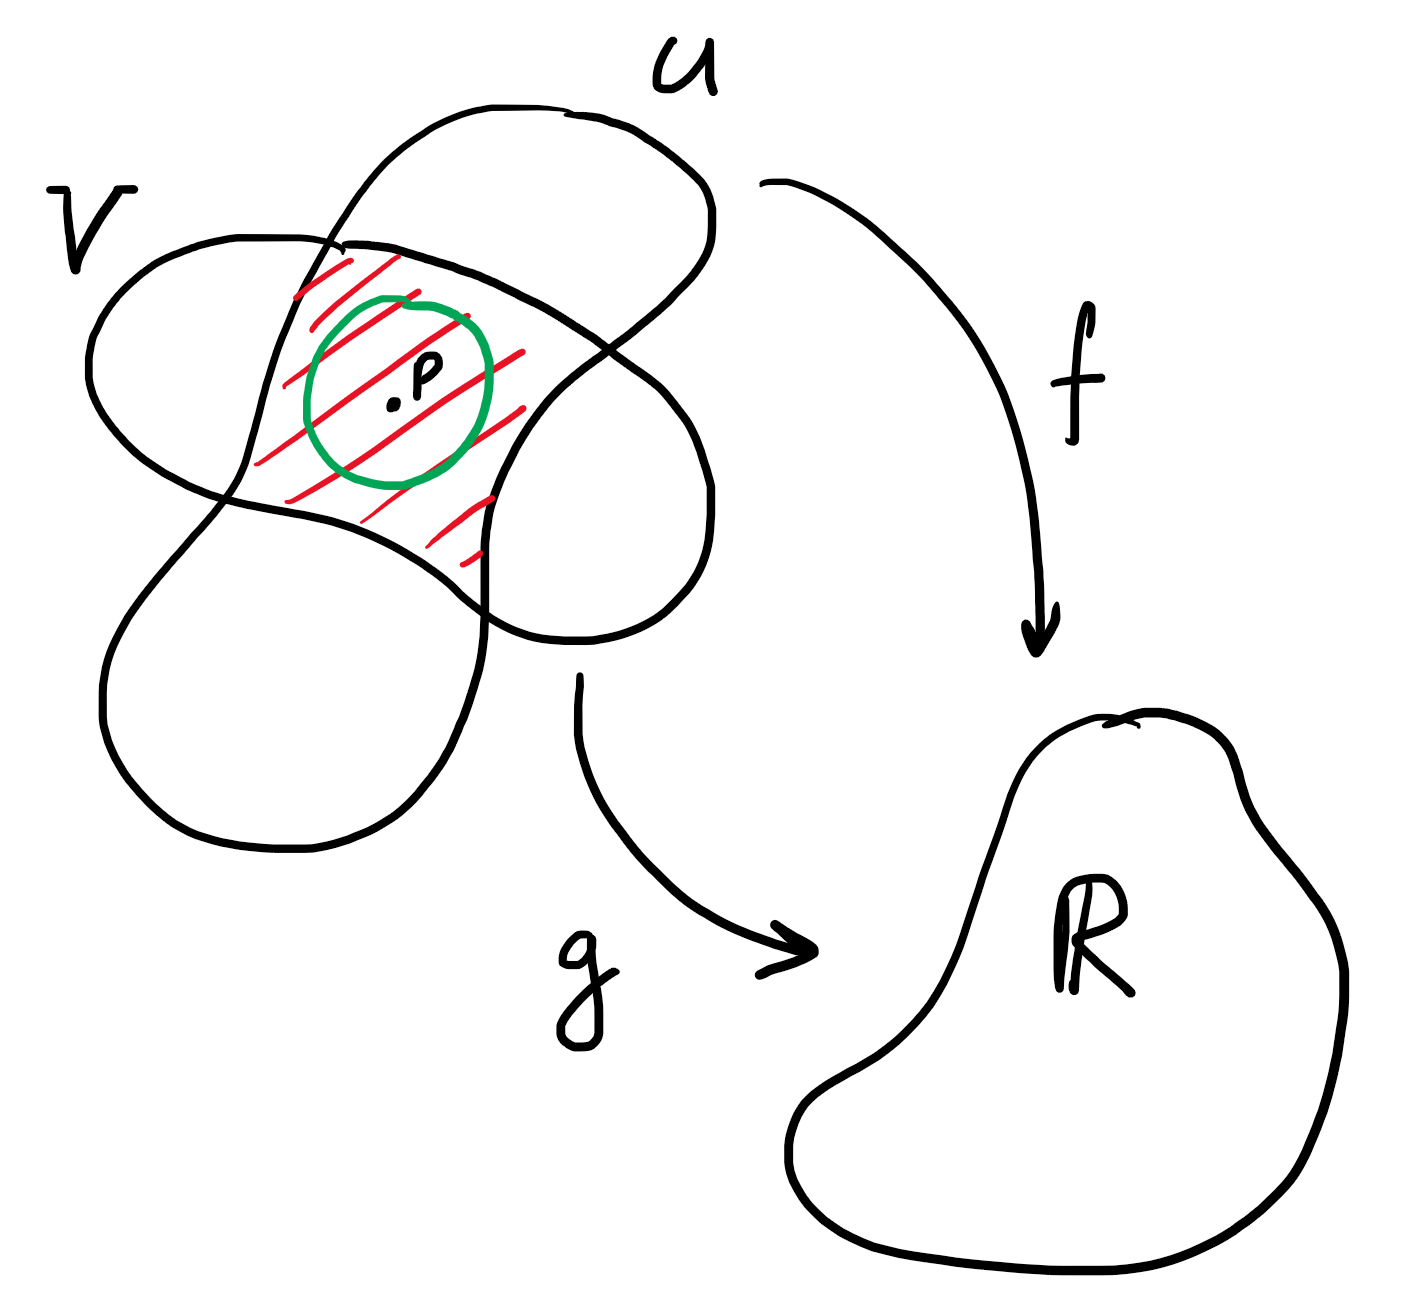
\includegraphics[width=0.4\textwidth,keepaspectratio]{img1}
\end{figure}

Definiamo ora l'insieme di coppie

\begin{equation}
	X \doteq \left\{ (f,U) \middle| f \in C^{\infty}(U), \, \text{$ U $ intorno di $ p $} \right\}
\end{equation}

Diciamo che\footnote{%
	Il simbolo $ \sim $ indica una relazione di equivalenza.%
} per $ p \in W $

\begin{equation}
	(f,U) \sim (g,V) \iff \exists W \subseteq U \cap V \mid f \equiv g \qq{in} W
\end{equation}

o equivalentemente

\begin{equation}
	(f,U) \sim (g,V) \iff \exists W \subseteq U \cap V \mid f(q) \equiv g(q), \forall q \in W
\end{equation}

Questa è effettivamente una relazione di equivalenza in quanto riflessiva, simmetrica e transitiva.\\
Prendiamo dunque lo spazio quoziente

\begin{equation}
	\sfrac{X}{\sim} \doteq C_{p}^{\infty}(\R^{n})
\end{equation}

dove un elemento $ [(f,U)] $ di questo spazio è chiamato \textit{germe} intorno al punto $ p $ ed è una \textit{classe di equivalenza} di coppie. A questo punto, $ C_{p}^{\infty}(\R^{n}) $ è l'insieme dei germi di funzioni $ C^{\infty} $ intorno a $ p $, i.e.

\begin{equation}
	C_{p}^{\infty}(\R^{n}) = \left\{ [(f,U)] \right\}
\end{equation} 

Possiamo definire un'applicazione

\map{D_{v}}%
	{C_{p}^{\infty}(\R^{n})}{\R}%
	{[(f,U)]}{D_{v} f}

Questa applicazione è ben definita in quanto l'associazione di un germe di funzioni ad un numero reale non dipende dal rappresentante scelto perché

\begin{equation}
	(f,U) \sim (g,V) \implies D_{v} g = D_{v} f
\end{equation}

\subsubsection{\textit{Esempio}}

Siano $ f $ e $ g $

\begin{equation}
	\begin{cases}
		f(x) = \dfrac{1}{1-x}, & x \in \R \setminus \{1\}\\\\
		g(x) = \displaystyle\sum_{j=1}^{+\infty} x^{j}, & x \in (-1,1)
	\end{cases}
\end{equation}

Nonostante $ f\neq g $, nell'intorno $ (-1,1) $ di $ p=0 $ vale l'equivalenza per i germi

\begin{equation}
	(f,\R \setminus \{1\}) \sim (g,(-1,1))
\end{equation}

in altre parole, le classi di equivalenza

\begin{equation}
	[(f,\R \setminus \{1\})] = [(g,(-1,1))] \in C_{0}^{\infty}(\R)
\end{equation}

\subsubsection{Algebra su campo $ \K $}

Un'algebra $ A $ su un campo $ \K $ è una coppia $ (V,\cdot) $ con $ V $ spazio vettoriale su $ \K $ (dunque con operazioni $ a+b \in A $ con $ a,b \in A $ e $ \lambda a \in A $ con $ \lambda \in \K $) e un'operazione binaria

\map{\cdot}%
	{A \times A}{A}%
	{(a,b)}{a \cdot b}

tale che soddisfi le condizioni\footnote{%
	In generale, non è necessaria l'associatività per definire un'algebra.}

\begin{equation}
	\begin{cases}
		(a \cdot b) \cdot c = a \cdot (b \cdot c) & \text{associatività}\\
		\begin{split}
			(a + b) \cdot c = a \cdot c + b \cdot c\\
			c \cdot (a + b) = c \cdot a + c \cdot b
		\end{split} & \text{distributività}\\
	\lambda (a \cdot b) = (\lambda a) \cdot b = a \cdot (\lambda b) & \text{omogeneità}
	\end{cases}
\end{equation}

per $ \forall a,b,c \in A $ e $ \forall \lambda \in \K $.\\
Equivalentemente, un algebra su un campo $ \K $ può essere pensata come un anello\footnote{%
	Le proprietà di associatività e distributività sono sufficienti per renderla un anello.%
} $ (A,+,\cdot) $ il quale sia anche uno spazio vettoriale tale che sia soddisfatta la proprietà di omogeneità.

\subsection{$ C_{p}^{\infty}(\R^{n}) $ come algebra su $ \R $}

Definiamo la somma

\begin{equation}
	[(f,U)] + [(g,V)] = [(f + g,U \cap V)]
\end{equation}

con $ [(f,U)], [(g,V)] \in C_{p}^{\infty}(\R^{n}) $. Questa somma è ben definita in quanto, prendendo altri due rappresentanti di $ [(f,U)] $ e $ [(g,V)] $, esiste sempre un intorno in cui questa somma sia definita.\\
Allo stesso modo, definiamo il prodotto

\begin{equation}
	[(f,U)] \cdot [(g,V)] = [(f g,U \cap V)]
\end{equation}

e la moltiplicazione per scalari

\begin{equation}
	\lambda [(f,U)] = [(\lambda f,U)]
\end{equation}

con $ \lambda \in \R $.\\
Tutte queste operazioni sono ben definite e soddisfano tutte le proprietà di un'algebra perché la somma, il prodotto e la moltiplicazione per uno scalare di funzioni $ C^{\infty} $ soddisfano queste stesse proprietà.\\
A questo punto si può dire che $ C_{p}^{\infty}(\R^{n}) $ sia un'algebra su $ \R $.\\
Nonostante non sia necessario per un'algebra, $ C_{p}^{\infty}(\R^{n}) $ è anche commutativa e unitaria\footnote{%
	Vedi Esercizio \ref{es1-7}.%
} su $ \R^{n} $.

\subsection{Derivazione puntuale di $ C_{p}^{\infty}(\R^{n}) $}

A questo punto, l'immagine dell'applicazione

\map{D}%
	{C_{p}^{\infty}(\R^{n})}{\R}%
	{[(f,U)]}{D_{v} f = \sum_{i=1}^{n} \pdv{f}{x^{i}} (p) \, v^{i}}

tale che:

\begin{enumerate}
	\item sia $ \R $-lineare\footnote{%
		Rispetto alla struttura di spazio vettoriale di $ C_{p}^{\infty}(\R^{n}) $.%
	}, cioè
		\begin{align}
			\begin{split}
				D ([(f,U)] + [(g,V)]) &= D ([(f,U)]) + D ([(g,V)])\\
				D (\lambda [(f,U)]) &= \lambda D ([(f,U)])
			\end{split}
		\end{align}
	
	\item soddisfi la \textit{regola di Leibniz}, cioè
		\begin{equation}
			D ([(f,U)] \cdot [(g,V)]) = D ([(f,U)]) \, g(p) + f(p) \, D ([(g,V)])
		\end{equation}
\end{enumerate}

è chiamata \textit{derivazione puntuale} dell'algebra $ C_{p}^{\infty}(\R^{n}) $.

\begin{proof}[Dimostrazione ($ \R $-linearità)]
	\begin{align}
		\begin{split}
			D ([(f,U)] + [(g,V)]) &= D ([(f+g,U \cap V)])\\
			&= D_{v} (f+g)\\
			&= \sum_{j=1}^{n} \dfrac{\partial (f+g)}{\partial x^{j}} (p) \, v^{j}\\
			&= \sum_{j=1}^{n} \dfrac{\partial f}{\partial x^{j}} (p) \, v^{j} + \sum_{j=1}^{n} \dfrac{\partial g}{\partial x^{j}} (p) \, v^{j}\\
			&= D ([(f,U)]) + D ([(g,V)])
		\end{split}
	\end{align}
\end{proof}

\begin{proof}[Dimostrazione ($ \R $-linearità)]
	\begin{align}
		\begin{split}
			\lambda D ([(f,U)]) &= D ([(\lambda f,U)])\\
			&= D_{v} (\lambda f)\\
			&= \sum_{j=1}^{n} \dfrac{\partial (\lambda f)}{\partial x^{j}} (p) \, v^{j}\\
			&= \lambda \sum_{j=1}^{n} \dfrac{\partial f}{\partial x^{j}} (p) \, v^{j}\\
			&= \lambda D ([(f,U)])
		\end{split}
	\end{align}
\end{proof}

\begin{proof}[Dimostrazione (Regola di Leibniz)]
	\begin{align}
		\begin{split}
			D ([(f,U)] \cdot [(g,V)]) &= D ([(f g,U \cap V)])\\
			&= D_{v} (f g)\\
			&= \sum_{j=1}^{n} \dfrac{\partial (f g)}{\partial x^{j}} (p) \, v^{j}\\
			&= \left( \sum_{j=1}^{n} \dfrac{\partial f}{\partial x^{j}} (p) \, v^{j} \right) \, g(p) + f(p) \left( \, \sum_{j=1}^{n} \dfrac{\partial g}{\partial x^{j}} (p) \, v^{j} \right)\\
			&= (D_{v} f) g(p) + f(p) (D_{v} g)\\
			&= D ([(f,U)]) \, g(p) + f(p) \, D ([(g,V)])
		\end{split}
	\end{align}
\end{proof}

Una derivazione è quindi un modo per associare ad un germe di funzioni un numero reale, soddisfacendo le proprietà definite sopra.\\
Indichiamo dunque l'insieme delle derivazioni di $ C_{p}^{\infty}(\R^{n}) $ come $ Der_{p}(C_{p}^{\infty}(\R^{n})) $.

\subsection{Isomorfismo tra $ T_{p}(\R^{n}) $ e $ Der_{p}(C_{p}^{\infty}(\R^{n})) $}

Definiamo l'applicazione

\begin{align}
	\begin{split}
		\phi : T_{p}(\R^{n}) &\to Der_{p}(C_{p}^{\infty}(\R^{n}))\\
		v &\mapsto D_{v}
	\end{split}
\end{align}

questa associa $ v \in T_{p}(\R^{n}) $ con $ p \in \R^{n} $ a $ D_{v} $, la quale è a sua volta un'applicazione che associa la classe di equivalenza di germi di funzioni $ [(f,U)] $ allo scalare

\begin{align}
	D_{v} f = \sum_{j=1}^{n} \dfrac{\partial f}{\partial x^{j}} (p) \, v^{j}
\end{align}

con $ v = [v^{1},\dots,v^{n}] $, dove $ D_{v} f $ è la derivata direzionale di $ f $ rispetto a $ v $; possiamo usare lo stesso simbolo per $ D_{v} ([(f,U)]) = D_{v} f $ perché questa relazione vale per qualsiasi rappresentante della classe.\\
L'applicazione $ \phi $ permette di considerare le derivazioni puntuali dell'algebra dei germi delle funzioni $ C_{p}^{\infty}(\R^{n}) $ al posto dell'insieme dei vettori che partono da un punto, in quanto questi due insiemi sono isomorfi tra loro. Utilizzare le derivazioni è utile perché, in termini di varietà differenziabile, non esiste una visualizzazione di uno spazio tangente.

\begin{theorem}
	L'applicazione $ \phi $ è un isomorfismo di spazi vettoriali, nello specifico tra $ T_{p}(\R^{n}) $ e $ Der_{p}(C_{p}^{\infty}(\R^{n})) $.
\end{theorem}

Per dimostrare questo teorema è necessario dimostrare innanzitutto che gli elementi $ D_{i} \in Der_{p}(C_{p}^{\infty}(\R^{n})) $ costituiscano uno spazio vettoriale, cioè devono valere

\begin{align}
	\begin{split}
		(D_{1} + D_{2}) ([(f,U)]) &= D_{1}([(f,U)]) + D_{2}([(f,U)])\\
		(\lambda D) ([(f,U)]) &= \lambda D ([(f,U)])
	\end{split}
\end{align}

per $ \forall D,D_{1},D_{2} \in Der_{p}(C_{p}^{\infty}(\R^{n})) $ e $ \forall \lambda \in \R $.\\
Vedi Esercizio \ref{es1-8}.

\begin{proof}[Dimostrazione ($ \R $-linearità)]
	\begin{align}
		\begin{split}
			(D_{1} + D_{2}) (\alpha [(f,U)] + \beta [(g,V)]) &= D_{1} (\alpha [(f,U)] + \beta [(g,V)]) +\\
			&+ \, D_{2} (\alpha [(f,U)] + \beta [(g,V)])\\
			&= \alpha D_{1} ([(f,U)]) + \beta D_{1} ([(g,V)]) +\\
			&+ \,\alpha D_{2} ([(f,U)]) + \beta D_{2} ([(g,V)])\\
			&= \alpha (D_{1} + D_{2}) ([(f,U)]) + \beta (D_{1} + D_{2}) ([(g,V)])
		\end{split}
	\end{align}

	per $ \alpha,\beta \in \R $.
\end{proof}

\begin{proof}[Dimostrazione (Regola di Leibniz)]
	\begin{align}
		\begin{split}
			(D_{1} + D_{2}) ([(f,U)] [(g,V)]) &= D_{1} ([(f,U)] [(g,V)]) + D_{2} ([(f,U)] [(g,V)])\\
			&= D_{1} ([(f,U)]) \, g(p) + f(p) \, D_{1} ([(g,V)]) +\\
			&+ \, D_{2} ([(f,U)]) \, g(p) + f(p) \, D_{2} ([(g,V)])\\
			&= (D_{1} + D_{2}) \{ ([(f,U)]) \, g(p) + f(p) \, ([(g,V)]) \}
		\end{split}
	\end{align}
\end{proof}

A questo punto, bisogna dimostrare che $ \phi $ sia $ \R $-lineare, iniettiva\footnote{%
	Un'applicazione $ f $ tra due insiemi $ A $ e $ B $ è \textit{iniettiva} se
	\begin{equation}
		\forall a_{1},a_{2} \in A \mid a_{1} \neq a_{2} \implies f(a_{1}) \neq f(a_{2})
	\end{equation}%
} e suriettiva\footnote{%
	Un'applicazione $ f $ tra due insiemi $ A $ e $ B $ è \textit{suriettiva} se
	\begin{equation}
		\forall b \in B, \, \exists a \in A \mid f(a) = b
	\end{equation}%
} perché venga considerata un isomorfismo.

\begin{proof}[Dimostrazione ($ \R $-linearità)]
	Sia $ [(f,U)] \in C_{p}^{\infty}(\R^{n}) $, possiamo scrivere
	
	\begin{align}
		\begin{split}
			D_{\alpha v + \beta w} ([(f,U)]) &= D_{\alpha v + \beta w} (f)\\
			&= \sum_{j=1}^{n} \dfrac{\partial f}{\partial x^{j}} (p) \, (\alpha v^{j} + \beta w^{j})\\
			&= \alpha \sum_{j=1}^{n} \dfrac{\partial f}{\partial x^{j}} (p) \, v^{j} + \beta \sum_{j=1}^{n} \dfrac{\partial f}{\partial x^{j}} (p) \, w^{j}\\
			&= \alpha D_{v} f + \beta D_{w} f\\
			&= \alpha D_{v} ([(f,U)]) + \beta D_{w} ([(f,U)])
		\end{split}
	\end{align}

	con $ \alpha,\beta \in \R $ e $ v,w \in T_{p}(\R^{n}) $.\\
	Da questo si ottiene
	
	\begin{align}
		\begin{split}
			\phi (\alpha v + \beta w) &= D_{\alpha v + \beta w}\\
			&= \alpha D_{v} + \beta D_{w}\\
			&= \alpha \phi (v) + \beta \phi (w)
		\end{split}
	\end{align}
\end{proof}

\begin{proof}[Dimostrazione (iniettività)]
	Consideriamo il \textit{kernel}\footnote{%
	Il \textit{kernel} o nucleo di un'applicazione, indicato con $ \ker $, è l'insieme di tutti e soli gli elementi del dominio che hanno come immagine lo $ 0 $ del codominio, i.e. nel caso considerato
	
	\begin{equation}
		\ker \phi = \left\{ v \in T_{p}(\R^{n}) \, \middle| \, \phi(v) \equiv D_{v} = 0 \right\}
	\end{equation}%
	} di $ \phi $: se questo contiene solo l'elemento $ 0 $, inteso come
	
	\begin{align}
		\begin{split}
			0 : C_{p}^{\infty}(\R^{n}) &\to \R\\
			[(f,U)] &\mapsto 0
		\end{split}
	\end{align}

	per $ \forall [(f,U)] \in C_{p}^{\infty}(\R^{n}) $.\\
	Se quindi $ \ker \phi = \{\} $ allora $ \phi $ è iniettiva.\\
	Siccome $ 0 $ associa un qualunque rappresentante della classe $ [(f,U)] $ sempre a $ 0 \in \R $, possiamo scegliere il germe $ [(x^{j},\R)] $, i.e.
	
	\begin{align}
		\begin{split}
			x^{j} : \R^{n} &\to \R\\
			(x^{1},\dots,x^{n}) &\mapsto x^{j}
		\end{split}
	\end{align}

	per $ \forall j=1,\dots,n $, la quale è una proiezione liscia dunque $ x^{j} \in C_{p}^{\infty}(\R^{n}) $. A questo punto
	
	\begin{align}
		\begin{split}
			0([(x^{j},\R)]) &= D_{v} ([(x^{j},\R)])\\
			&= D_{v} (x^{j})\\
			&= \sum_{i=1}^{n} \dfrac{\partial x^{j}}{\partial x^{i}} (p) \, v^{i}\\
			&= \sum_{i=1}^{n} \delta^{ij} \, v^{i}\\
			&= v^{j}
		\end{split}
	\end{align}

	perciò $ v^{j} = 0 $ per $ \forall j=1,\dots,n $ dunque se $ v \in \ker \phi \implies v = 0 \in T_{p}(\R^{n}) $.
\end{proof}

La suriettività implica che se si fissa una qualunque derivazione puntuale esiste uno spazio tangente che mandato tramite $ \phi $ dà quella derivazione. In simboli

\begin{equation}
	\forall D \in Der_{p} (C_{p}^{\infty}(\R^{n})), \, \exists v \in T_{p}(\R^{n}) \, \mid \, \phi(v) = D
\end{equation}

dove $ \phi = D_{v} $.\\
Dobbiamo quindi trovare un $ v $ tale che faccia coincidere $ D \equiv D_{v} $.\\
Prima di farlo, enunciamo il seguente lemma:

\begin{lemma}[Derivata di costante]
	Sia la funzione
	
	\begin{align}
		\begin{split}
			c : \R^{n} &\to \R^{n}\\
			x &\mapsto c
		\end{split}
	\end{align}

	e sia $ D \in Der_{p} (C_{p}^{\infty}(\R^{n})) $. Allora
	
	\begin{equation}
		D([(c,\R^{n})]) = 0
	\end{equation}
\end{lemma}

\begin{proof}[Dimostrazione (lemma)]
	\begin{align}
		\begin{split}
			D([(c,\R^{n})]) &= D([(1 c,\R^{n})])\\
			&= c \, D([(1,\R^{n})])\\
			&= c \, D([(1 \cdot 1,\R^{n})])\\
			&= c \, \{D([(1,\R^{n})]) \, 1 + 1 \, D([(1,\R^{n})])\}\\
			&= 2 c \, D([(1,\R^{n})])\\
			&= \, 0
		\end{split}
	\end{align}
\end{proof}

A questo punto possiamo dimostrare la suriettività di $ \phi $:

\begin{proof}[Dimostrazione (suriettività)]
	Due funzioni sono uguali se e solo se coincidono per ogni punto del dominio, i.e.
	
	\begin{equation}
		D_{v} = D \iff D_{v}([(f,U)]) = D([(f,U)]), \quad \forall ([(f,U)]) \in (C_{p}^{\infty}(\R^{n}))
	\end{equation}

	Per dimostrarlo, possiamo scegliere un rappresentante arbitrario della classe $ [(f,U)] $ in quanto $ D_{v}([(f,U)]) = D_{v} f $ e possiamo prendere il dominio $ U $ stellato rispetto a $ p $, perciò per il teorema di Taylor con resto
	
	\begin{equation}
		f(x) = f(p) + \sum_{i=1}^{n} (x^{i}-p^{i}) \, g_{i}(x)
	\end{equation}

	per $ \forall x \in U $ e $ \forall g_{i} \in C^{\infty}(U) $ con
	
	\begin{equation}
		g_{i}(p) = \dfrac{\partial f}{\partial x^{i}} (p), \quad i=1,\dots,n
	\end{equation}

	Sia $ v = [v^{1},\dots,v^{n}] $ definito come $ v^{j} = D([(x^{j},\R)]) $ per $ \forall j=1,\dots,n $.\\
	Ora applichiamo $ D $ a $ f $
	
	\begin{align}
		\begin{split}
			D ([(f,U)]) &= D ([(f(p),\R^{n})]) + D \left(\left[\left( \sum_{i=1}^{n} (x^{i}-p^{i}) \, g_{i}(x) , U \right)\right]\right)\\
			&= D \left(\left[\left( \sum_{i=1}^{n} (x^{i}-p^{i}) \, g_{i}(x) , U \right)\right]\right)\\
			&= \sum_{i=1}^{n} D ([( (x^{i}-p^{i}) \, g_{i}(x) , U )])\\
			&= \sum_{i=1}^{n} \left\{ D ([( (x^{i}-p^{i}), U )]) \, g_{i}(p) + (p^{i}-p^{i}) \, D ([( g_{i}(x), U )]) \right\}\\
			&= \sum_{i=1}^{n} D ([( (x^{i}-p^{i}), U )]) \, g_{i}(p)\\
			&= \sum_{i=1}^{n} \left\{ D ([( x^{i}, U )]) - D ([( p^{i}, U )]) \right\} g_{i}(p)\\
			&= \sum_{i=1}^{n} D ([( x^{i}, U )]) \, g_{i}(p)\\
			&= \sum_{i=1}^{n} D ([( x^{i}, U )]) \, \dfrac{\partial f}{\partial x^{i}} (p)\\
			&= \sum_{i=1}^{n} \dfrac{\partial f}{\partial x^{i}} (p) \, v^{i}\\
			&= D_{v} f\\
			&= D_{v} ([(f,U)])
		\end{split}
	\end{align}

	per $ \forall [(f,U)] \in C_{p}^{\infty}(\R^{n}) $.
\end{proof}

Date queste proprietà di $ \phi $, questa applicazione è un omeomorfismo tra $ T_{p}(\R^{n}) $ e $ Der_{p}(C_{p}^{\infty}(\R^{n})) $, i.e.

\begin{equation}
	T_{p}(\R^{n}) \simeq Der_{p}(C_{p}^{\infty}(\R^{n}))
\end{equation}

\begin{corollary}
	\begin{equation}
		\dim ( T_{p}(\R^{n}) ) = n = \dim ( Der_{p}(C_{p}^{\infty}(\R^{n})) )
	\end{equation}
\end{corollary}

\subsection{Base canonica per $ Der_{p}(C_{p}^{\infty}(\R^{n})) $}

L'insieme delle $ n $-uple

\begin{equation}
	\left( \left. \dfrac{\partial}{\partial x^{1}} \right|_{p},\dots,\left. \dfrac{\partial}{\partial x^{n}} \right|_{p} \right)
\end{equation}

i cui elementi sono definiti come

\begin{equation}
	\left. \dfrac{\partial}{\partial x^{j}} \right|_{p} ([(f,U)]) = \dfrac{\partial f}{\partial x^{j}} (p), \quad \forall p \in U
\end{equation}

forma una base per lo spazio $ Der_{p}(C_{p}^{\infty}(\R^{n})) $.

\begin{proof}
	Essendo $ T_{p}(\R^{n}) \simeq Der_{p}(C_{p}^{\infty}(\R^{n})) $, da cui
	
	\begin{equation}
		\dim ( Der_{p}(C_{p}^{\infty}(\R^{n})) ) = n
	\end{equation}
		
	se $ e_{1},\dots,e_{n} $ è la base canonica\footnote{%
		Con $ (e_{j})_{k} = \delta_{jk} $, e.g. $ e_{3} = (0,0,1,0,\dots,0) $.%
	} di $ T_{p}(\R^{n}) $, si ha che

	\begin{equation}
		\phi(e_{i}) = D_{e_{i}}, \quad \forall i=1,\dots,n
	\end{equation}

	Applicando questo ad una funzione $ f $
	
	\begin{align}
		\begin{split}
			D_{e_{i}} (f) &= \sum_{j=1}^{n} \dfrac{\partial f}{\partial x^{j}} (p) \, (e_{i})_{j}\\
			&= \sum_{j=1}^{n} \dfrac{\partial f}{\partial x^{j}} (p) \, \delta_{ij}\\
			&= \dfrac{\partial f}{\partial x^{i}} (p)
		\end{split}
	\end{align}
\end{proof}

\section{Campi di vettori su aperti di $ \R^{n} $}

Prendiamo un aperto $ U \in \R^{n} $ con $ n \geqslant 1 $, un \textit{campo di vettori} su $ U $ è un'applicazione

\begin{align}
	\begin{split}
		X : U &\to \bigsqcup_{p \in U} T_{p}(\R^{n})\\
		p &\mapsto X_{p}
	\end{split}
\end{align}

dove il codominio è l'\textit{unione disgiunta} degli spazi di vettori tangenti in ogni punto di $ \R^{n} $; inoltre $ T_{p}(\R^{n}) = T_{p}(U) $ in quanto le due algebre seguenti coincidono $ C_{p}^{\infty}(\R^{n}) = C_{p}^{\infty}(U) $ perché i germi delle funzioni sono definiti localmente, quindi non dipendono dall'aperto considerato.\\
Un elemento del campo di vettori può essere scritto in funzione della base canonica di $ T_{p}(\R^{n}) $

\begin{equation}
	X_{p} = \sum_{i=1}^{n} a^{i}(p) \, \left. \dfrac{\partial}{\partial x^{i}} \right|_{p}
\end{equation}

dove $ a^{i}(p) \in \R $ con $ i=1,\dots,n $. In modo naturale, l'elemento $ X_{p} $ si identifica con l'$ n $-upla $ X_{p} = [a^{1}(p),\dots,a^{n}(p)] $.\\
Il campo di vettori $ X $ (senza la valutazione in un punto $ p $) si scrive come

\begin{equation}
	X = \sum_{i=1}^{n} a^{i} \, \dfrac{\partial}{\partial x^{i}}
\end{equation}

dove ora $ a^{i} $ è una funzione $ a^{i} : U \to \R $.

\subsection{Campi di vettori lisci}

Un campo di vettori $ X $ è $ C^{\infty} $ (liscio o differenziabile) se, scritto nella forma

\begin{equation}
	X = \sum_{i=1}^{n} a^{i} \, \dfrac{\partial}{\partial x^{i}}
\end{equation}

le funzioni $ a^{i} $ sono lisce, i.e. $ a^{i} \in C^{\infty}(U) $ con $ \forall i=1,\dots,n $.\\
L'insieme dei campi di vettori che rispettano questa prescrizione è chiamato $ \chi(U) $.

\subsubsection{\textit{Esempi}}

\paragraph{1.}

\begin{align}
	\begin{split}
		X : U = \R^{2} \setminus \{(0,0)\} &\to T_{(x,y)}(\R^{2})\\
		(x,y) &\mapsto X = - \dfrac{x}{\sqrt{x^{2}+y^{2}}} \dfrac{\partial}{\partial x} - \dfrac{y}{\sqrt{x^{2}+y^{2}}} \dfrac{\partial}{\partial y}
	\end{split}
\end{align}

\begin{figure}[H]
	\centering
	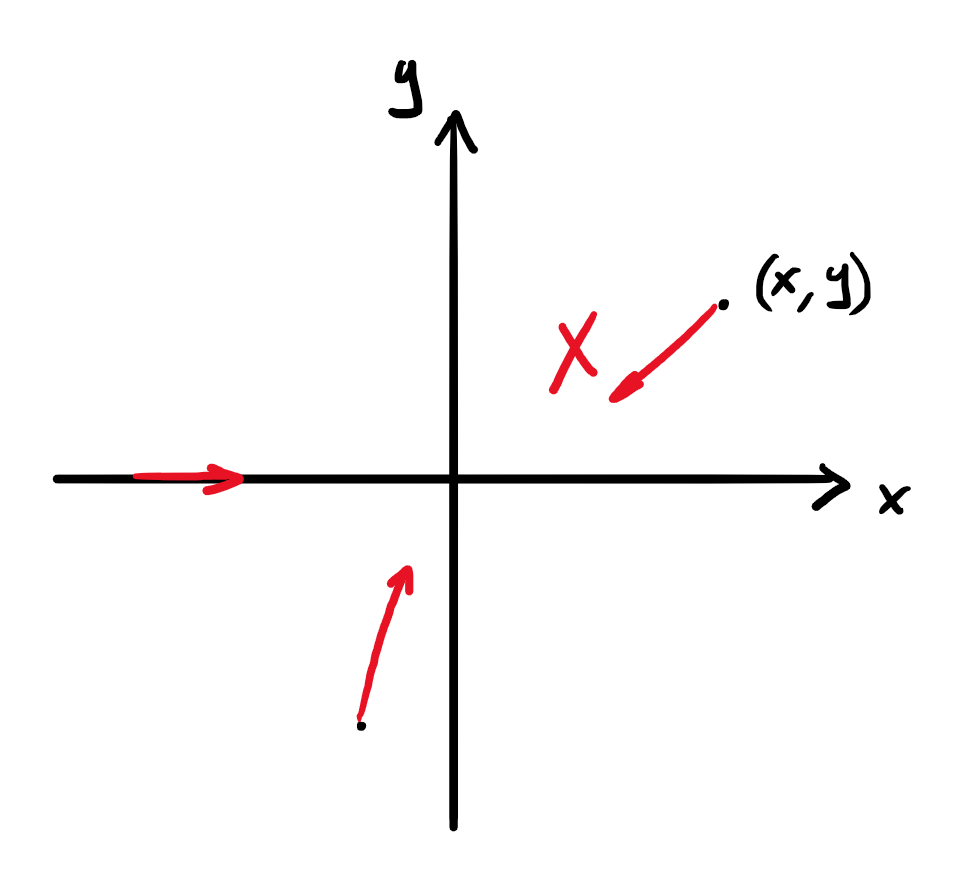
\includegraphics[width=0.4\textwidth,keepaspectratio]{img2}
\end{figure}

Questo campo è liscio perché qualsiasi derivata non annulla mai il denominatore in quanto l'origine non è compresa.

\paragraph{2.}

\begin{align}
	\begin{split}
		X : U = \R^{2} \setminus \{(0,0)\} &\to T_{(x,y)}(\R^{2})\\
		(x,y) &\mapsto X = - \dfrac{y}{\sqrt{x^{2}+y^{2}}} \dfrac{\partial}{\partial x} - \dfrac{x}{\sqrt{x^{2}+y^{2}}} \dfrac{\partial}{\partial y}
	\end{split}
\end{align}

\begin{figure}[H]
	\centering
	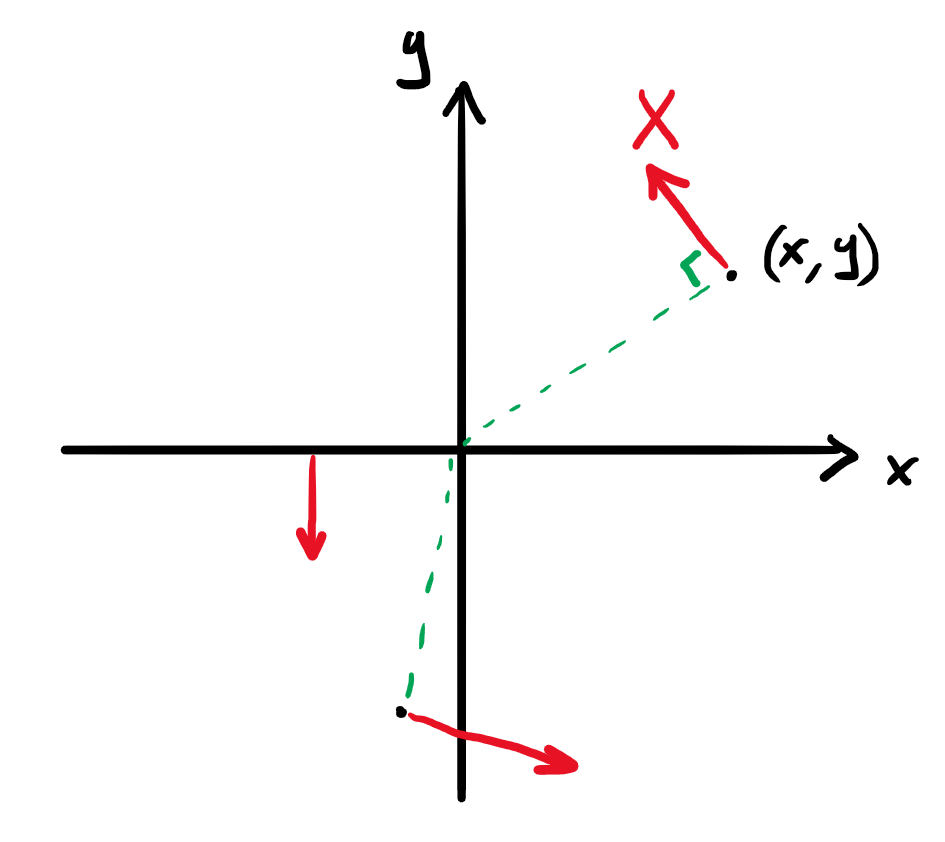
\includegraphics[width=0.4\textwidth,keepaspectratio]{img3}
\end{figure}

Questo campo è liscio perché qualsiasi derivata non annulla mai il denominatore in quanto l'origine non è compresa.

\subsection{Operazioni in $ \chi(U) $}

Si può definire la somma come

\begin{equation}
	(X+Y)_{p} \doteq X_{p} + Y_{p}
\end{equation}

con $ X,Y \in \chi(U) $, questo significa che se

\begin{align}
	\begin{split}
		X &= \sum_{i=1}^{n} a^{i} \, \dfrac{\partial}{\partial x^{i}}\\\\
		Y &= \sum_{i=1}^{n} b^{i} \, \dfrac{\partial}{\partial x^{i}}
	\end{split}
\end{align}

con $ a^{i},b^{i} \in C^{\infty}(U) $, allora

\begin{equation}
	X+Y = \sum_{i=1}^{n} (a^{i}+b^{i}) \, \dfrac{\partial}{\partial x^{i}}
\end{equation}

dove ancora $ a^{i}+b^{i} \in C^{\infty}(U) $ con $ \forall i=1,\dots,n $.\\
Si può definire anche la moltiplicazione per scalari come

\begin{equation}
	(\lambda X)_{p} \doteq \lambda X_{p}
\end{equation}

con $ X \in \chi(U) $ e $ \lambda \in \R $, questo significa che se

\begin{equation}
	X = \sum_{i=1}^{n} a^{i} \, \dfrac{\partial}{\partial x^{i}}
\end{equation}

con $ a^{i} \in C^{\infty}(U) $, allora

\begin{equation}
	\lambda X = \sum_{i=1}^{n} (\lambda a^{i}) \, \dfrac{\partial}{\partial x^{i}}
\end{equation}

dove ancora $ \lambda a^{i} \in C^{\infty}(U) $ con $ \forall i=1,\dots,n $.\\
L'ultima operazione è quella di moltiplicazione di un campo di vettori per un'altra funzione

\begin{equation}
	(f X)_{p} \doteq f(p) X_{p}
\end{equation}

con $ X \in \chi(U) $ e $ f \in C^{\infty}(U) $, questo significa

\begin{equation}
	f X = \sum_{i=1}^{n} (f a^{i}) \, \dfrac{\partial}{\partial x^{i}}
\end{equation}

dove ancora $ f a^{i} \in C^{\infty}(U) $ con $ \forall i=1,\dots,n $.\\
Le prime due operazioni dotano l'insieme di $ \chi(U) $ della proprietà di spazio vettoriale.\\
Osserviamo che $ C^{\infty}(U) $ è un anello commutativo unitario.

\subsection{$ \chi(U) $ come $ C^{\infty}(U) $-modulo}

\subsubsection{$ \R $-modulo sinistro}

Sia $ R $ un anello commutativo unitario, un gruppo abeliano $ (A,+) $ è detto $ R $\textit{-modulo sinistro} se esiste un'applicazione

\begin{align}
	\begin{split}
		\cdot : R \times A &\to A\\
		(r,a) &\mapsto r \cdot a
	\end{split}
\end{align}

tale che

\begin{equation}
	\begin{cases}
		1_{R} \cdot a = a\\
		r \cdot (s \cdot a) = (r s) \cdot a\\
		(r+s) \cdot a = r \cdot a + s \cdot a\\
		r \cdot (a+b) = r \cdot a + r \cdot b
	\end{cases}
\end{equation}

per $ \forall r,s \in R $ e $ \forall a,b \in A $. Queste proprietà valgono solo da \textit{sinistra}, potrebbero non valere se calcolate da destra.

\subsubsection{$ \R $-modulo destro}

Sia $ R $ un anello commutativo unitario, un gruppo abeliano $ (A,+) $ è detto $ R $\textit{-modulo destro} se esiste un'applicazione

\begin{align}
	\begin{split}
		* : A \times R &\to A\\
		(a,r) &\mapsto a * r
	\end{split}
\end{align}

tale che

\begin{equation}
	\begin{cases}
		a * 1_{R} = a\\
		(a*r)*s = a*(r s)\\
		a*(r+s) = a*r + a*s\\
		(a+b)*r = a*r + b*r
	\end{cases}
\end{equation}

per $ \forall r,s \in R $ e $ \forall a,b \in A $. Queste proprietà valgono solo da \textit{destra}, potrebbero non valere se calcolate da sinistra.\\\\
Da queste definizioni, si dice che $ (A,+) $ è un $ R $-modulo se è un $ R $-modulo sinistro e destro, con $ \cdot \equiv * $.

\begin{remark}
	Se un gruppo $ A $ è un $ R $-modulo e $ R $ è un campo $ \K $, allora $ A $ è uno spazio vettoriale in $ \K $.
\end{remark}

\begin{theorem}\label{chi-mod}
	$ (\chi(U),+) $ è un $ C^{\infty}(U) $-modulo.
\end{theorem}

\begin{proof}
	Per dimostrare che $ (\chi(U),+) $ sia un $ C^{\infty}(U) $-modulo, è necessario dimostrare che la seguente applicazione (commutativa)
	
	\map{K}%
		{C^{\infty}(U) \times \chi(U)}{\chi(U)}%
		{(f,X)}{f X}

	sia liscia.\\
	Vedi Esercizio \ref{es1-9}.\\
	Devono dunque essere verificate queste proprietà\footnote{%
		Nonostante l'applicazione sia commutativa, scriveremo la funzione sempre a sinistra dei campi, per notazione.%
	}:

	\begin{equation}
		\begin{cases}
			1_{C^{\infty}(U)} \cdot X = X\\
			f \cdot (g \cdot X) = (f g) \cdot X\\
			f \cdot (X+Y) = f \cdot X + f \cdot Y\\
			(f+g) \cdot X = f \cdot X + g \cdot X
		\end{cases}
	\end{equation}

	per $ \forall f,g \in C^{\infty}(U) $ e $ \forall X,Y \in \chi(U) $.
\end{proof}

\subsection{Derivata di funzione rispetto ad un campo di vettori} 

I campi di vettori permettono di derivare funzioni, così come è possibile fare la derivata direzionale di una funzione rispetto ad un vettore e dunque rispetto ad un campo di vettori.\\
Prendiamo $ X \in \chi(U) $ con $ U \subset \R^{n} $ aperto e $ f \in C^{\infty}(U) $. Definisco la derivata di $ f $ rispetto ad $ X $ come $ X f \in C^{\infty}(U) $. La derivata puntuale è definita come $ (X f) (p) = X_{p} f $ con $ p \in U $: se il campo è

\begin{equation}
	X = \sum_{i=1}^{n} a^{i} \dfrac{\partial}{\partial x^{i}}
\end{equation}

allora

\begin{align}
	\begin{split}
		(X f) (p) &= \left( \sum_{i=1}^{n} a^{i}(p) \, \dfrac{\partial}{\partial x^{i}} \right) (f)\\
		&= \sum_{i=1}^{n} a^{i}(p) \, \dfrac{\partial f}{\partial x^{i}} (p)
	\end{split}
\end{align}

perciò

\begin{align}
	\begin{split}
		X f : U \to& \R\\
		p \mapsto& \sum_{i=1}^{n} a^{i}(p) \, \dfrac{\partial f}{\partial x^{i}} (p)
	\end{split}
\end{align}

Questa applicazione è $ C^{\infty}(U) $ perché lo è $ (X f) (p) $, la quale lo è a sua volta perché $ X \in \chi(U) $ in quanto $ a^{i} \in C^{\infty}(U) $ e $ f \in C^{\infty}(U) $.\\
Posso considerare l'applicazione

\begin{align}
	\begin{split}
		X : C^{\infty}(U) &\to C^{\infty}(U)\\
		f &\mapsto X f
	\end{split}
\end{align}

ricordando che $ C^{\infty}(U) $, oltre ad essere un anello commutativo unitario, è un'algebra sui reali, perciò l'applicazione $ X $ è $ \R $-lineare. Inoltre, siccome $ X_{p} \in Der_{p}(C_{p}^{\infty}(\R^{n})) $, soddisfa la regola di Leibniz

\begin{align}
	\begin{split}
		X (f g) (p) &= X_{p} (f g)\\
		&= (X_{p} f) \, g(p) + f(p) \, (X_{p} g) 
	\end{split}
\end{align}

perciò anche l'applicazione $ X $ soddisfa la regola di Leibniz

\begin{equation}
	X (f g) = (X f) \, g + f \, (X g)
\end{equation}

\subsubsection{Derivazione di un'algebra}

Sia $ A $ un'algebra\footnote{%
	Un'algebra è costituita da $ (\text{spazio vettoriale},\cdot) $, dove l'operazione
		\begin{align}
			\begin{split}
				\cdot : A \times A &\to A\\
				(a,b) &\mapsto a \cdot b
			\end{split}
		\end{align}
	soddisfa le proprietà
	\begin{equation}
		\begin{cases}
			(a \cdot b) \cdot c = a \cdot (b \cdot c) & \text{associatività}\\
			\begin{split}
				(a + b) \cdot c = a \cdot c + b \cdot c\\
				c \cdot (a + b) = c \cdot a + c \cdot b
			\end{split} & \text{distributività}\\
			\lambda (a \cdot b) = (\lambda a) \cdot b = a \cdot (\lambda b) & \text{omogeneità}
		\end{cases}
	\end{equation}
	per $ \forall a,b,c \in A $ e $ \forall \lambda \in \R $.%
} su un campo $ \K $, un'applicazione $ D : A \to A $ che sia $ \K $-lineare e tale che soddisfi la regola di Leibniz

\begin{equation}
	D (a \cdot b) = (D a) \cdot b + a \cdot (D b)
\end{equation}

per $ \forall a,b \in A $, è chiamata \textit{derivazione dell'algebra} $ A $. L'insieme di tutte le derivazioni di un'algebra $ A $ viene indicato come $ Der(A) $.\\
Vedi Esercizi \ref{es1-10} e \ref{es1-11}.

\subsection{Campo di vettori liscio come derivazione dell'algebra $ C^{\infty}(U) $}

Possiamo vedere un campo di vettori come una derivazione di un'algebra, quindi definiamo un'applicazione

\begin{align}
	\begin{split}
		\phi : \chi(U) &\to Der(C^{\infty}(U))\\
		X &\mapsto \phi(X)
	\end{split}
\end{align}

in cui

\begin{equation}
	\phi(X) (f) \doteq X f
\end{equation}

Sia $ \chi(U) $ che $ Der(C^{\infty}(U)) $ sono $ C^{\infty}(U) $-modulo, dall'applicazione

\begin{align}
	\begin{split}
		K : C^{\infty}(U) \times Der(C^{\infty}(U)) &\to Der(C^{\infty}(U))\\
		(f,D) &\mapsto f D
	\end{split}
\end{align}

da cui

\begin{equation}
	(f D) (g) = f (D g)
\end{equation}

Inoltre $ \phi $ è anche $ C^{\infty}(U) $-lineare, i.e

\begin{equation}
	\phi(f X + g Y) = f \, \phi(X) + g \, \phi(Y)
\end{equation}

per $ \forall f,g \in C^{\infty}(U) $ e $ \forall X,Y \in \chi(U) $.\\
Dimostreremo per le varietà differenziabili che $ \phi $ è un isomorfismo di $ C^{\infty}(U) $-moduli, i.e. $ \chi(U) \simeq Der(C^{\infty}(U)) $.\\
Tramite questo isomorfismo, si possono identificare i campi di vettori lisci con le derivazioni dell'algebra delle funzioni lisce, analogamente a come lo spazio tangente ad un punto di $ \R^{n} $ si può identificare con le derivazioni puntuali dell'algebra dei germi delle funzioni in quel punto, i.e. $ T_{p}(\R^{n}) \simeq Der_{p}(C_{p}^{\infty}(\R^{n})) $.

%

\chapter{Varietà differenziabili}
\section{Varietà topologiche e differenziabili}

\subsection{Varietà topologiche}

Sia $ X $ uno spazio topologico\footnote{%
	Cioè un insieme non vuoto a cui è abbinata una topologia.%
}, diremo che $ X $ è una \textit{varietà topologica} se sono soddisfatte le seguenti condizioni:

\begin{itemize}
	\item $ X $ è $ T_{2} $ o \textit{di Hausdorff}, i.e. dati due punti distinti di $ X $ è sempre possibile trovare due intorni disgiunti che contengano i due punti
	
	\item $ X $ è $ N_{2} $ o a base numerabile, i.e. esiste una base per la topologia di $ X $ che sia numerabile
	
	\item $ X $ è localmente euclideo, i.e. per $ \forall p \in X $ esiste un aperto $ U \ni p $ ed esiste un'applicazione $ \phi : U \to \R^{n} $ tale che $ \phi : U \to \phi(U) \subset \R^{n} $ aperto sia un omeomorfismo, dunque localmente ogni aperto di $ X $ è omeomorfo a un aperto di $ \R^{n} $
\end{itemize}

La coppia $ (U,\phi) $ è chiamata \textit{carta} intorno a $ p $; nel caso in cui $ \phi(p)=0 $, la carta è detta \textit{centrata} in $ p $.\\
Diremo che, se lo spazio topologico è localmente omeomorfo a $ \R^{n} $, la sua dimensione è pari a $ \dim (X) = n $.

\begin{remark}
	Possiamo sempre assumere che $ \phi(U) \equiv \R^{n} $. Questo perché all'interno dell'immagine di $ U $ in $ \R^{n} $ (i.e. $ \phi(U) $) è sempre possibile trovare una palla $ B_{\delta}(0) $ centrata nell'origine con raggio $ \delta $ opportuno per la quale esista sempre un diffeomorfismo (e quindi un omeomorfismo) $ h : B_{\delta}(0) \to \R^{n} $.\\
	Sia la carta $ (V,\psi) $ con $ V = \phi^{-1}(B_{\delta}(0)) $ aperto e $ \psi = h \circ \left. \phi \right|_{V} $ in cui $ \psi : V \to \R^{n} $ è un omeomorfismo: da questo si ottiene che, cambiando $ U $ e $ \phi $ se necessario, si può sempre assumere che l'immagine della carta sia $ \R^{n} $, dunque $ \psi(V) = \R^{n} $.
	
	\img{0.4}{img4}
\end{remark}

Il vantaggio di avere una carta su uno spazio topologico è quello di poterlo ricondurre, almeno localmente, ad $ \R^{n} $.

\begin{remark}
	Se $ (U,\phi) $ è una carta su $ X $
	
	\begin{align}
		\begin{split}
			\phi(p) = (0,\dots,0) \in \R^{n}\\
			\phi(q) = (x^{1}(q),\dots,x^{n}(q)) \in \R^{n}
		\end{split}
	\end{align}

	con $ p,q \in U $ e $ x^{i} : U \to \R $.
\end{remark}

\begin{remark}
	Il teorema di invarianza topologica della dimensione, i.e.
	
	\begin{equation}
		U \simeq V \implies \dim V = \dim U
	\end{equation}

	rende ben definita la dimensione di una varietà topologica.
\end{remark}

\`{E} importante precisare che le tre condizioni che determinano uno spazio topologico sono indipendenti tra di loro, dunque due di queste non implicano necessariamente la terza.

\subsubsection{Unione disgiunta di spazi topologici}

Sia $ \{A_{j}\}_{j \in J} $ una famiglia di spazi topologici e sia\footnote{%
	L'unione disgiunta equivale ad un'unione in cui ogni insieme ha un indice diverso, e.g. l'insieme non connesso $ (0,1) \sqcup (0,1) $ è diverso da $ (0,1) \cup (0,1) = (0,1) $.}

\begin{align}
	\begin{split}
		A &= \bigsqcup_{j \in J} A_{j}\\
		&= \bigcup_{j \in J} A_{j} \times \{j\}
	\end{split}
\end{align}

Definisco la topologia dell'unione disgiunta su $ A $ dichiarando $ U $ aperto in $ A $ se e solo se $ U \cap A_{j} $ è aperto in $ A_{j} $ per $ \forall j \in J $.\\
Vedi Esercizio \ref{BONUS2-1}.

\subsubsection{\textit{Esempi}}

\paragraph{1. Spazio $ N_{2} + T_{2} $ ma non localmente euclideo} 

Sia l'insieme degli assi coordinati

\begin{equation}
	X = \{ (x,y) \in \R^{2} \mid x,y = 0 \}
\end{equation}

questo spazio è $ N_{2} + T_{2} $ in quanto sottospazio di $ \R^{2} $ il quale ha queste proprietà\footnote{%
	La proprietà di uno spazio di essere $ N_{2} + T_{2} $ è \textit{ereditaria}.%
}, ma non è localmente euclideo nell'origine. Perché lo sia, deve essere possibile prendere un intorno dell'origine $ U $ il quale sia omeomorfo ad $ \R^{n} $, ma se si toglie un punto da entrambi gli spazi, questi dovrebbero essere ancora omeomorfi, nello specifico togliamo l'origine (supponendo che l'origine di $ U $ vada nell'origine di $ \R^{n} $) quindi $ U \setminus \{(0,0)\} \simeq \R^{n} \setminus \{0\} $: se $ n=1 $, lo spazio $ \R^{n} \setminus \{0\} $ è composto da due componenti connesse mentre, se $ n \geqslant 2 $, $ \R^{n} \setminus \{0\} $ è connesso. Dunque non è omeomorfo a $ U \setminus \{(0,0)\} $ in quanto questo spazio è formato da 4 componenti connesse e, dalla topologia, due spazi omeomorfi inducono una bigezione tra le parti connesse.

\begin{figure}[H]
	\centering
	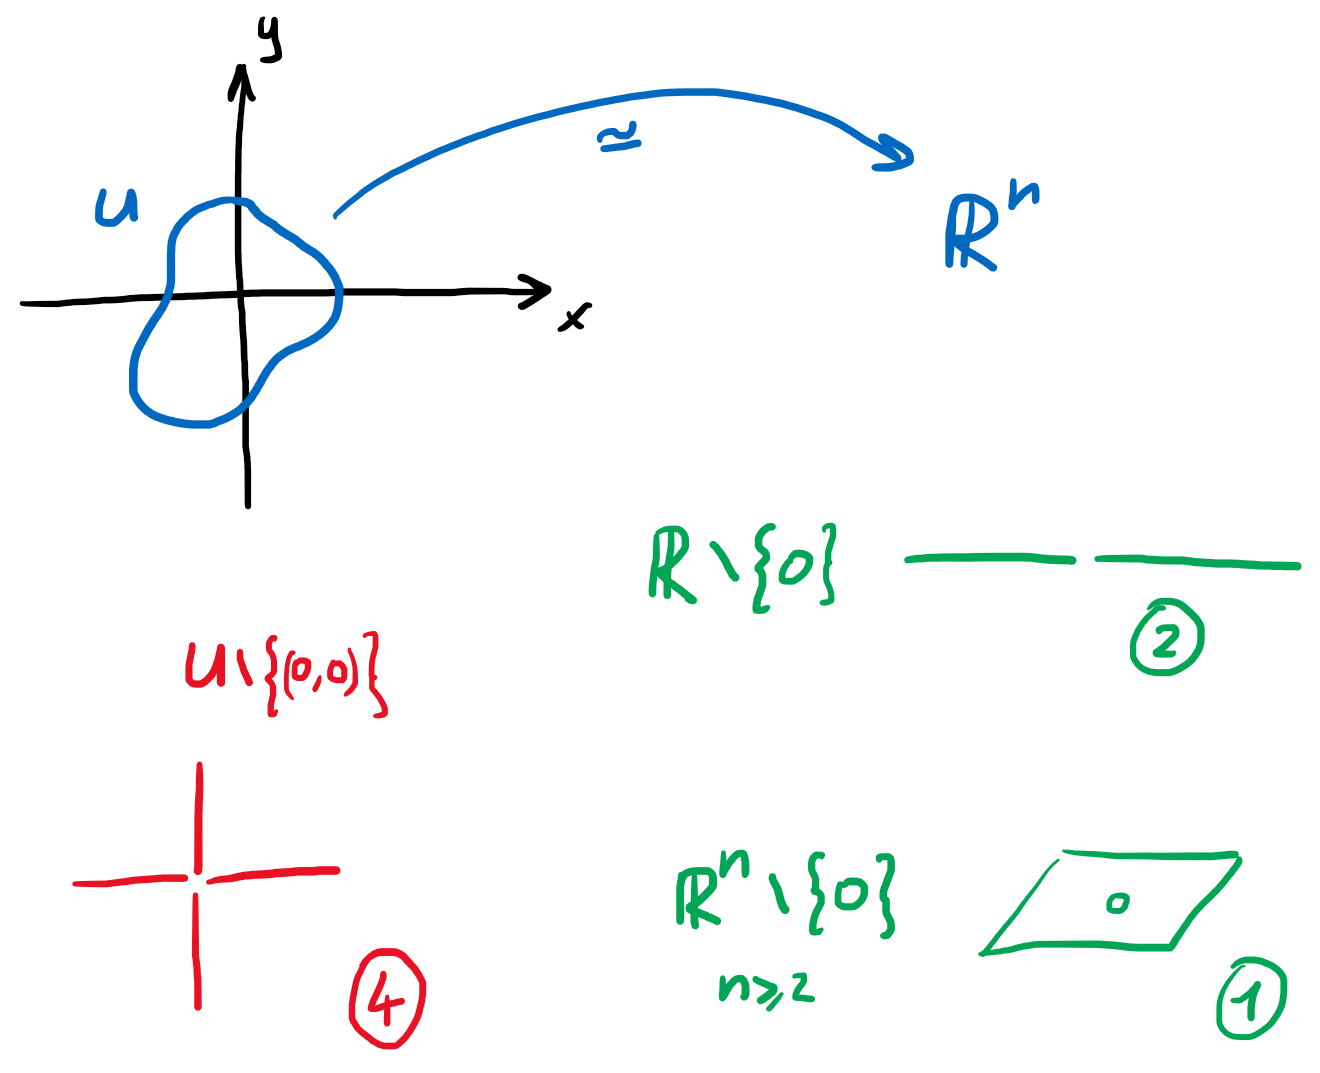
\includegraphics[width=0.4\textwidth,keepaspectratio]{img5}
\end{figure}

\paragraph{2. Spazio $ T_{2} $ e localmente euclideo ma non $ N_{2} $}

Consideriamo l'unione disgiunta

\begin{align}
	\begin{split}
		X &= \bigsqcup (0,1)\\
		&= \bigcup_{j \in J} (0,1) \times \{j\}
	\end{split}
\end{align}

con $ J $ non numerabile.\\
Questo spazio non è $ N_{2} $ perché non esiste una base numerabile per infinite coppie non numerabili.\\
Prendendo due punti qualunque di $ X $: questi o stanno entrambi nello stesso $ (0,1) $, il quale è di Hausdorff, quindi $ X $ è $ T_{2} $; oppure stanno in due intervalli diversi, i quali sono due intervalli disgiunti che contengono i due punti, quindi $ X $ è ancora $ T_{2} $.\\
Lo spazio $ X $ è localmente euclideo perché un suo punto $ p $ sarà contenuto in uno degli intervalli $ (0,1) \times \{j_{0}\} $ il quale è omeomorfo ad $ \R $.

\paragraph{3. Spazio $ N_{2} $ e localmente euclideo ma non $ T_{2} $ (retta con due origini)}

Sia $ S = \R \setminus \{0\} \cup \{A\} \cup \{B\} $ dove $ A,B \notin \R \setminus \{0\} $.\\ 
Per associare a questo spazio una topologia, possiamo trovare una famiglia di sottoinsiemi che faccia da base per la topologia (generata da questa famiglia). Sia\footnote{%
	$ \mathcal{P}(E) $ indica l'insieme di tutti i sottoinsiemi di $ E $.%
} $ \mathfrak{B} \subset \mathcal{P} (S) $ con

\begin{equation}
	\mathfrak{B} = \left\{ (a,b) \, \middle| \, a<b, \, 0 \notin (a,b) \right\} \cup \left\{ I_{A}(c,d) \right\} \cup \left\{ I_{B}(c,d) \right\}
\end{equation}

con $ c,d \in \R^{+} $ e

\begin{equation}
	\begin{cases}
		I_{A}(c,d) = (-c,0) \cup \{A\} \cup (0,d)\\
		I_{B}(c,d) = (-c,0) \cup \{B\} \cup (0,d)
	\end{cases}
\end{equation}

Se l'intersezione di elementi di $ \mathfrak{B} $ può essere scritta come unioni di elementi di $ \mathfrak{B} $, allora esiste un'unica topologia $ \tau_{\mathfrak{B}} $ generata da $ \mathfrak{B} $ che ha questa come base.\\
L'intersezione tra intervalli di tipo $ (a,b) $ produce intervalli dello stesso tipo, quella tra intervalli $ (a,b) $ e $ I_{A}(c,d) $ produce ancora un intervallo euclideo che appartiene alla famiglia, per il caso

\begin{equation}
	I_{A}(c,d) \cap I_{A}(c^{\prime},d^{\prime}) =%
		\begin{cases}
			I_{A}(c^{\prime},d)\\
			I_{A}(c,d^{\prime})\\
			I_{A}(c^{\prime},d^{\prime})\\
			I_{A}(c,d)
		\end{cases}
\end{equation}

e analogamente per $ I_{A}(c,d) \cap I_{B}(c',d') $, il risultato è l'unione di elementi di $ \mathfrak{B} $.\\
Vogliamo dunque mostrare che lo spazio, insieme alla sua topologia, $ (S,\tau_{\mathfrak{B}}) $ sia $ N_{2} $ e localmente euclideo ma non $ T_{2} $.\\
Se consideriamo la topologia di $ S $ ristretta\footnote{%
	$ \R \setminus \{0\} \subset S $ perché una base per $ \tau_{eucl.} $ è $ \mathfrak{B}_{\R \setminus \{0\}} = \left\{ (a,b) \, \middle| \, a<b, \, 0 \notin (a,b) \right\} \subset \mathfrak{B} $.%
} a $ \R \setminus \{0\} \subset S $ otteniamo che $ \tau_{\left. \mathfrak{B} \right|_{\R \setminus \{0\}}} = \tau_{euclidea} $, possiamo quindi trovare una famiglia numerabile tale che ogni intervallo della forma $ (a,b) $ possa essere scritto come unione di questa famiglia numerabile proprio perché $ \R \setminus \{0\} $ è $ N_{2} $, i.e.

\begin{equation}
	(a,b) = \bigcup_{r,s \in \Q} (r,s)
\end{equation}

dove $ \Q $ indica i numeri razionali e $ 0 \notin (r,s) $; analogamente

\begin{align}
	\begin{split}
		I_{A}(c,d) &= \bigcup_{r,s \in \Q} I_{A}(r,s)\\
		I_{B}(c,d) &= \bigcup_{r,s \in \Q} I_{B}(r,s)
	\end{split}
\end{align}

A questo punto possiamo prendere la famiglia

\begin{equation}
	\mathfrak{C} = \left\{ (r,s) \, \middle| \, r,s \in \Q \, \wedge \, 0 \notin (r,s) \right\} \cup \left\{ I_{A}(r,s) \, \middle| \, r,s \in \Q^{+} \right\} \cup \left\{ I_{B}(r,s) \, \middle| \, r,s \in \Q^{+} \right\}
\end{equation}

la quale è una base numerabile e dunque $ S $ è $ N_{2} $.\\
Mostriamo che $ (S,\tau_{\mathfrak{B}}) $ sia localmente euclideo, costruendo un'applicazione

\begin{align}
	\begin{split}
		\phi : I_{A}(c,d) &\to (-c,d) \subset \R\\
		x &\mapsto x\\
		A &\mapsto 0
	\end{split}
\end{align}

la quale è un omeomorfismo, perché è una bigezione continua. Per la continuità, prendiamo un intervallo $ (e,f) \subset (-c,d) $ con $ 0 \notin (e,f) $ la cui controimmagine è sé stesso, i.e. $ \phi^{-1}((e,f)) = (e,f) \in \tau_{\mathfrak{B}} $; se invece $ (-e,f) $ con $ e,f>0 $, la sua controimmagine sarà $ \phi^{-1}((-e,f)) = I_{A}(e,f) \in \tau_{\mathfrak{B}} $ il quale è un aperto. Per mostrare che $ \phi $ sia effettivamente continua dobbiamo verificare che la sua inversa $ \phi^{-1} $ sia anch'essa continua, ma è equivalente a mostrare che $ \phi $ sia aperta\footnote{%
	Un'applicazione aperta associa aperti ad aperti.%
}: sia che si prenda un intervallo $ (e,f) $ oppure $ I_{A}(e,f) $, si ottiene come immagine comunque un aperto, perciò è continua e lo spazio è localmente euclideo.\\
Infine troviamo che $ (S,\tau_{\mathfrak{B}}) $ non è $ T_{2} $ perché due aperti di questo spazio che contengono $ A $ e $ B $ rispettivamente si devono necessariamente intersecare, i.e. vale sempre $ I_{A}(c,d) \cap I_{B}(e,f) \neq \{\} $.

\subsection{Atlanti}

\subsubsection{Atlanti topologici}

Sia $ M $ uno spazio topologico, un \textit{atlante topologico su} $ M $ è una famiglia di carte $ \{(U_{\alpha},\phi_{\alpha})\}_{\alpha \in A} $ tali che

\begin{equation}
	\bigcup_{\alpha \in A} U_{\alpha} = M
\end{equation}

i.e. la famiglia delle carte è un \textit{ricoprimento} dello spazio topologico, il quale è localmente euclideo.

\subsubsection{Compatibilità tra carte}

Due carte $ (U,\phi) $ e $ (V,\psi) $ di uno spazio topologico $ M $ sono $ C^{\infty} $\textit{-compatibili} se le applicazioni

\begin{align}
	\begin{split}
		\phi \circ \psi^{-1} : \psi(U \cap V) &\to \phi(U \cap V)\\
		\psi \circ \phi^{-1} : \phi(U \cap V) &\to \psi(U \cap V)
	\end{split}
\end{align}

sono lisce.

\begin{figure}[H]
	\centering
	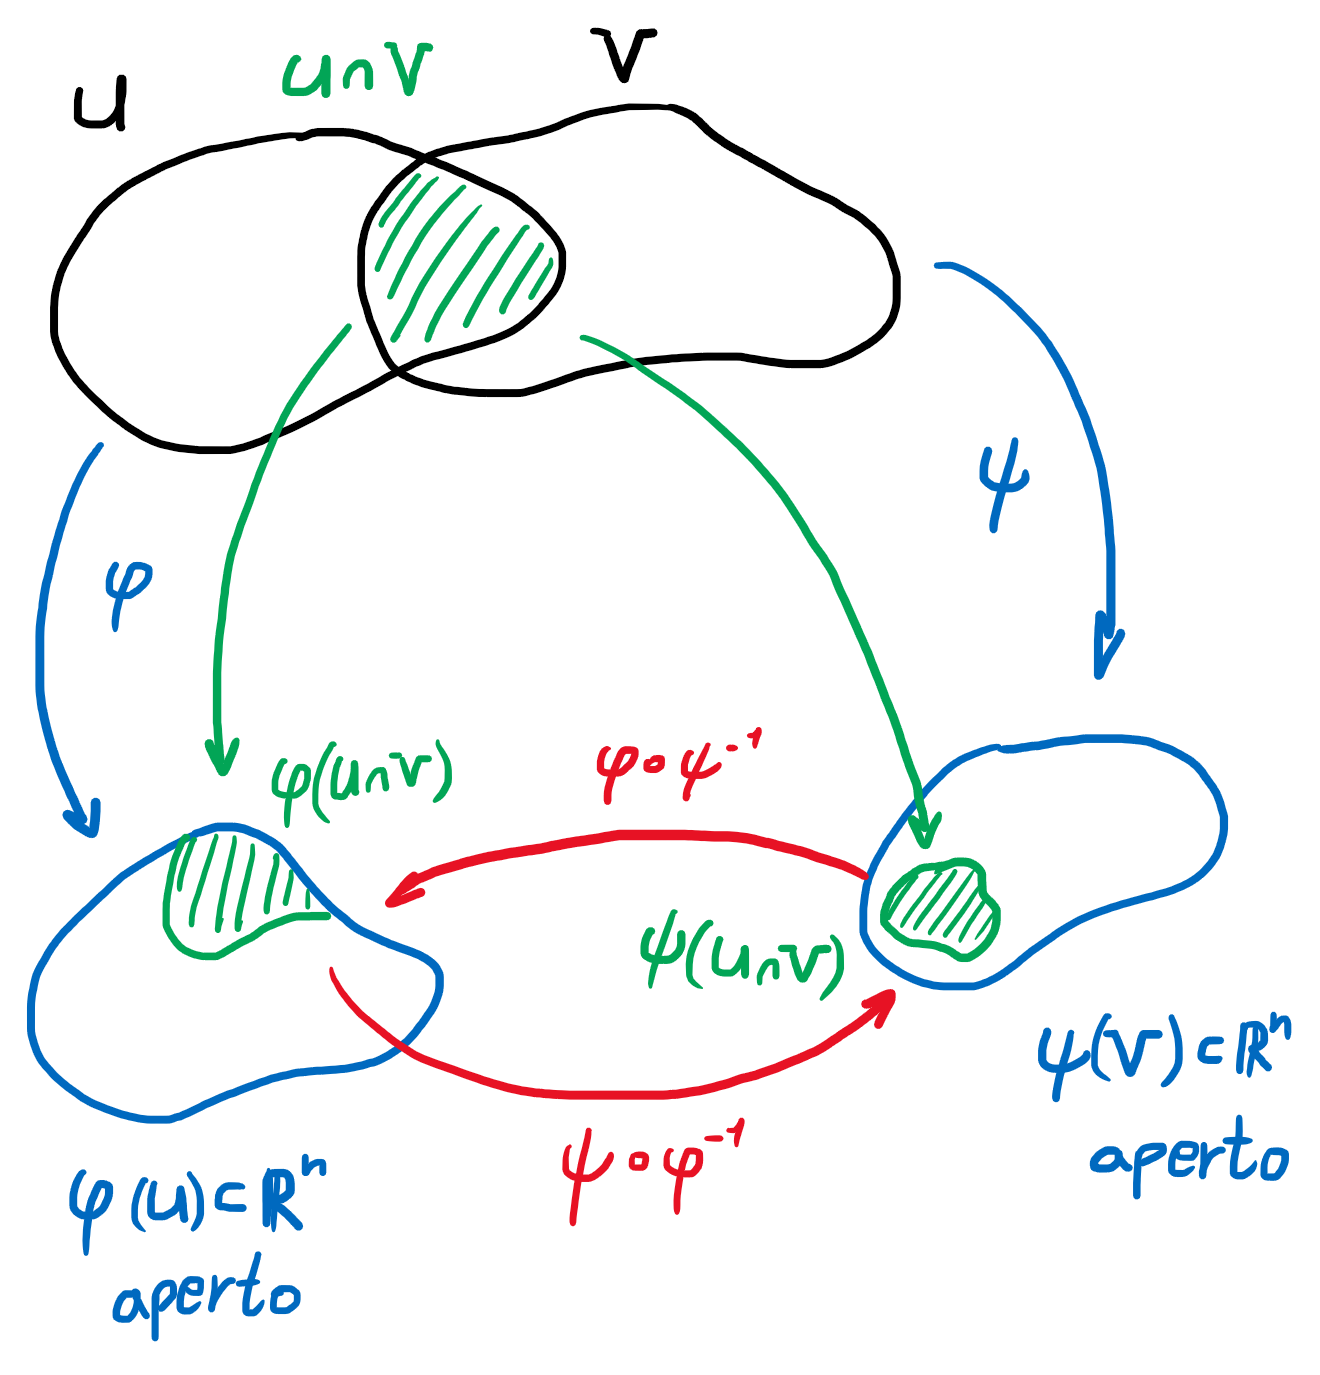
\includegraphics[width=0.4\textwidth,keepaspectratio]{img6}
\end{figure}

\begin{remark}
	La $ C^{\infty} $-compatibilità è automaticamente verificata se $ U \cap V = \{\} $.
\end{remark}

\begin{remark}
	La proprietà di $ C^{\infty} $-compatibilità è riflessiva e simmetrica ma non transitiva, i.e.
	
	\begin{itemize}
		\item Se $ (U,\phi) $ è $ C^{\infty} $-compatibile con $ (V,\psi) $ allora $ (V,\psi) $ è $ C^{\infty} $-compatibile con $ (U,\phi) $
		
		\item $ (U,\phi) $ è $ C^{\infty} $-compatibile con $ (U,\phi) $
		
		\item Se $ (U_{1},\phi_{1}) $ è $ C^{\infty} $-compatibile con $ (U_{2},\phi_{2}) $ e se $ (U_{2},\phi_{2}) $ è $ C^{\infty} $-compatibile con $ (U_{3},\phi_{3}) $, non è detto che $ (U_{1},\phi_{1}) $ e $ (U_{3},\phi_{3}) $ siano $ C^{\infty} $-compatibili
	\end{itemize}
\end{remark}

Per le prime due condizioni della transitività, definendo $ U_{ij} \doteq U_{i} \cap U_{j} $ e $ U_{ijk} \doteq U_{i} \cap U_{j} \cap U_{k} $ con $ i,j,k=1,2,3 $, le seguenti applicazioni sono lisce

\begin{align}
	\begin{split}
		\phi_{1} \circ \phi_{2}^{-1} : \phi_{2}(U_{12}) &\to \phi_{1}(U_{12})\\
		\phi_{2} \circ \phi_{1}^{-1} : \phi_{1}(U_{12}) &\to \phi_{2}(U_{12})\\
		\phi_{2} \circ \phi_{3}^{-1} : \phi_{3}(U_{23}) &\to \phi_{2}(U_{23})\\
		\phi_{3} \circ \phi_{2}^{-1} : \phi_{2}(U_{23}) &\to \phi_{3}(U_{23})
	\end{split}
\end{align}

e dovrebbero esserlo anche

\begin{align}
	\begin{split}
		\phi_{1} \circ \phi_{3}^{-1} : \phi_{3}(U_{13}) &\to \phi_{1}(U_{13})\\
		\phi_{3} \circ \phi_{1}^{-1} : \phi_{1}(U_{13}) &\to \phi_{3}(U_{13})
	\end{split}
\end{align}

scrivendo

\begin{align}
	\begin{split}
		\phi_{3} \circ \phi_{1}^{-1} &= \phi_{3} \circ (\phi_{2}^{-1} \circ \phi_{2}) \circ \phi_{1}^{-1}\\
		&= (\phi_{3} \circ \phi_{2}^{-1}) \circ (\phi_{2} \circ \phi_{1}^{-1})
	\end{split}
\end{align}

l'applicazione $ \phi_{3} \circ \phi_{2}^{-1} $ è $ C^{\infty}(\phi_{2}(U_{23})) $ e $ \phi_{2} \circ \phi_{1}^{-1} $ è $ C^{\infty}(\phi_{1}(U_{12})) $ dunque $ \phi_{3} \circ \phi_{1}^{-1} $ è sicuramente $ C^{\infty}(\phi_{1}(U_{123})) $ ma non sappiamo a priori il suo comportamento in $ \phi_{1}(U_{13} \setminus U_{123}) $, dunque non possiamo dire che $ \phi_{3} \circ \phi_{1}^{-1} $ sia $ C^{\infty} $ e perciò la $ C^{\infty} $-compatibilità non è transitiva.\\\\
%
Sia $ \mathfrak{U} = \{(U_{\alpha},\phi_{\alpha})\} $ un atlante topologico di uno spazio $ M $, diremo che $ (V,\psi) $ carta di $ M $ è $ C^{\infty} $-compatibile con $ \mathfrak{U} $ se $ (V,\psi) $ è $ C^{\infty} $-compatibile con $ (U_{\alpha},\phi_{\alpha}) $ per $ \forall \alpha \in A $.\\\\
%
Sia $ \mathfrak{U} $ un atlante topologico su $ M $, se due carte $ (V,\psi) $ e $ (W,\sigma) $ sono $ C^{\infty} $-compatibili con $ \mathfrak{U} $ allora $ (V,\psi) $ è $ C^{\infty} $-compatibile con $ (W,\sigma) $.

\begin{proof}[Dimostrazione (transitività tramite atlante)]
	Vogliamo dimostrare che le due applicazioni
	
	\begin{align}
		\begin{split}
			\psi \circ \sigma^{-1} : \phi(V \cap W) &\to \psi(V \cap W)\\
			\sigma \circ \psi^{-1} : \psi(V \cap W) &\to \sigma(V \cap W)
		\end{split}
	\end{align}

	siano lisce.\\
	Prendiamo $ \sigma \circ \psi^{-1} $: questa è liscia se, per $ \forall p \in V \cap W $, $ \sigma \circ \psi^{-1} $ è liscia in $ \psi(p) \in \psi(V \cap W) $.\\
	Essendo l'atlante $ \mathfrak{U} $ un ricoprimento di $ M $, esisterà una carta $ (U_{\alpha},\phi_{\alpha}) \ni p $ dunque $ p \in U_{\alpha} \cap V \cap W $: potendo scrivere $ \sigma \circ \psi^{-1} = \sigma \circ \phi_{\alpha}^{-1} \circ \phi_{\alpha} \circ \psi^{-1} $ questa è automaticamente liscia in $ \psi(U_{\alpha} \cap V \cap W) $.\\
	Questo conclude la dimostrazione perché abbiamo trovato un aperto che contiene il punto, i.e. $ p \in U_{\alpha} \cap V \cap W $ per $ p $ arbitrario, in cui l'applicazione sia liscia, la quale è una proprietà locale.
	
\end{proof}

\subsection{Varietà differenziabili}

Sia $ M $ uno spazio topologico, un atlante topologico $ \mathfrak{U} = \{(U_{\alpha},\phi_{\alpha})\} $ è detto $ C^{\infty} $ (liscio o differenziabile) se $ (U_{\alpha},\phi_{\alpha}) $ è $ C^{\infty} $-compatibile con $ (U_{\beta},\phi_{\beta}) $ per $ \forall \alpha,\beta $.\\
Diremo che un atlante differenziabile $ \mathfrak{M} = \{(U_{\alpha},\phi_{\alpha})\} $ è \textit{massimale} se per qualunque altro atlante differenziabile $ \mathfrak{M}^{\prime} $ di $ M $ si ha che

\begin{equation}
	\mathfrak{M} \subset \mathfrak{M}^{\prime} \implies \mathfrak{M} = \mathfrak{M}^{\prime}
\end{equation}

Dato $ M $ spazio topologico, una \textit{struttura differenziabile} su $ M $ è la scelta di un atlante massimale per $ M $.\\
Una \textit{varietà differenziabile} è una varietà topologica con una struttura differenziabile $ \mathfrak{M} $.\\
Diciamo che una varietà differenziabile ha dimensione $ n $ se questa è la dimensione della varietà topologica sottostante\footnote{%
	Vale il teorema di invarianza della dimensione differenziabile.%
}.\\\\
%
Qualunque sia l'atlante differenziabile su una varietà topologica è sempre possibile trovare un atlante massimale unico che lo contiene, cioè

\begin{definition}
	Sia $ \mathfrak{U} $ un atlante differenziabile su uno spazio topologico $ M $, allora esiste ed è unica la struttura differenziale (o atlante massimale) $ \mathfrak{M} $ su $ M $ tale che contenga $ \mathfrak{U} \subset \mathfrak{M} $.
\end{definition}

\begin{proof}
	Consideriamo la famiglia $ \mathfrak{M} = \mathfrak{U} \cup \{(V_{i},\psi_{i})\}_{i \in I} $ dove $ \mathfrak{U} $ è un atlante differenziabile e $ \{(V_{i},\psi_{i})\}_{i \in I} $ è un insieme di carte $ C^{\infty} $-compatibili con l'atlante. Per la proposizione precedente, $ \mathfrak{M} $ è un atlante differenziabile di $ M $ perché, se tutte le carte $ \{(V_{i},\psi_{i})\}_{i \in I} $ sono compatibili con l'atlante allora sono compatibili tra di loro, dunque $ \mathfrak{M} \supset \mathfrak{U} $.\\
	Per dimostrare che $ \mathfrak{M} $ sia un atlante massimale, prendiamo $ \mathfrak{M}' $ atlante differenziabile di $ M $ tale che $ \mathfrak{M} \subset \mathfrak{M}' $: se $ \mathfrak{M}' \supset \mathfrak{M} $ allora $ \mathfrak{M}' \supset \mathfrak{U} $, quindi tutte le carte di $ \mathfrak{M}' $ sono $ C^{\infty} $-compatibili con $ \mathfrak{U} $, perciò per definizione $ \mathfrak{M} \supset \mathfrak{M}' $, dimostrando che $ \mathfrak{M}' = \mathfrak{M} $ e quindi che $ \mathfrak{M} $ sia massimale.\\
	Per dimostrare che $ \mathfrak{M} $ sia l'unico atlante massimale tale che $ \mathfrak{M} \supset \mathfrak{U} $, prendiamo $ \mathfrak{M}' $ un altro atlante differenziabile massimale di $ M $ tale che $ \mathfrak{M} \supset \mathfrak{U} $, allora tutte le carte di $ \mathfrak{M}' $ sono $ C^{\infty} $-compatibili con $ \mathfrak{U} $ e quindi, per definizione, $ \mathfrak{M}' \supset \mathfrak{M} $ ma, siccome $ \mathfrak{M}' $ è massimale, questo implica che $ \mathfrak{M} = \mathfrak{M}' $.
\end{proof}

\begin{remark}
	Siano $ M $ una varietà differenziabile, $ (U_{\beta},\phi_{\beta}) $ una carta della struttura differenziabile e $ V \subset U_{\beta} $ un aperto di $ M $, allora $ (V,\phi) $ (dove $ \phi $ è la restrizione della funzione $ \phi_{\beta} $ all'aperto $ V $, i.e. $ \phi = \left. \phi_{\beta} \right|_{V} $) è una carta per $ M $ per la struttura differenziabile fissata.
\end{remark}

Infatti, se prendiamo l'atlante massimale differenziabile $ \mathfrak{M} = \{(U_{\alpha},\phi_{\alpha})\} $ e consideriamo $ \phi \circ \phi_{\alpha}^{-1} $

\begin{align}
	\begin{split}
		\phi \circ \phi_{\alpha}^{-1} : \phi_{\alpha}(U_{\alpha} \cap V) &\to \phi(U_{\alpha} \cap V)\\
		\phi_{\alpha} \circ \phi^{-1} : \phi(U_{\alpha} \cap V) &\to \phi_{\alpha}(U_{\alpha} \cap V)
	\end{split}
\end{align}

vediamo che queste sono $ C^{\infty} $-compatibili con l'atlante perché

\begin{align}
	\begin{split}
		\phi \circ \phi_{\alpha}^{-1} &= \left. \phi_{\beta} \circ \phi_{\alpha}^{-1} \right|_{\phi_{\alpha}(U_{\alpha} \cap V)}\\
		\phi_{\alpha} \circ \phi^{-1} &= \left. \phi_{\alpha} \circ \phi_{\beta}^{-1} \right|_{\phi(U_{\alpha} \cap V)}\\
	\end{split}
\end{align}

sono le restrizioni ad un aperto di funzioni $ C^{\infty} $-compatibili e dunque appartengono all'atlante massimale.\\
In particolare, se $ U $ è un aperto qualunque di $ M $ e $ (U_{\beta},\phi_{\beta}) $ una carta della struttura differenziabile, allora $ (U \cap U_{\beta},\left. \phi_{\beta} \right|_{U \cap U_{\beta}}) $ è una carta nella struttura differenziabile.

\subsubsection{\textit{Esempi}}

\paragraph{0. $ \R^{n} $}

Considero $ (\R^{n},\id_{\R^{n}}) $: questo è un atlante differenziabile per $ \R^{n} $ ($ N_{2}+T_{2} $, aspetti topologici) che contiene l'unica carta $ (\R^{n},\id_{\R^{n}}) $.\\
Essendoci un atlante differenziale per lo spazio, esisterà un'unica struttura differenziabile su $ \R^{n} $ di cui $ (\R^{n},\id_{\R^{n}}) $ è una carta.

\paragraph{1. Aperto di varietà differenziabile}

Siano $ M $ una varietà differenziabile e $ U \subset M $ un suo aperto, allora $ U $ è una varietà differenziabile, con struttura indotta da $ M $, tale che $ \dim (U) = \dim (M) $.\\
Infatti se $ \mathfrak{U} = \{(U_{\alpha},\phi_{\alpha})\} $ è un atlante differenziabile su $ M $ (massimale o no), allora $ \mathfrak{V} = \{(U_{\alpha} \cap U,\left. \phi_{\alpha} \right|_{U_{\alpha} \cap U})\} $ è un atlante differenziabile per $ U $.

\paragraph{2. Varietà 0-dimensionali}

Essendo $ \R^{0} = \{0\} $, siccome deve esistere un omeomorfismo dall'intorno del punto a $ 0 $, questo intorno sarà costituito dal solo punto. La varietà sarà dunque costituita da un insieme di punti con \textit{topologia discreta}, i.e. ogni punto è aperto. Uno spazio discreto è sempre $ T_{2} $ e, per questo spazio, la base è numerabile.\\
La condizione di $ C^{\infty} $-compatibilità è automatica perché gli aperti sono sempre disgiunti.

\paragraph{3. Curve}

Per le curve differenziabili, $ \dim (M) = 1 $. Poniamo $ M $ connessa, sapendo che

\begin{theorem}
	\begin{equation}
		M \text{ curva connessa } \implies M = \R \, \lor \, M = \S^{1}
	\end{equation}

	cioè, se $ M $ è una curva connessa, allora è la retta reale $ \R $ oppure il cerchio unitario $ \S^{1} $.
\end{theorem}

\paragraph{4. Superfici}

Per le superfici differenziabili\footnote{%
	Le \textit{parametrizzazioni} $ X $ di curve e superfici sono l'inverso delle carte $ \phi = X^{-1} $, i.e per la parametrizzazione di una superficie
	
	\map{X}%
		{U \subset \R^{2}}{\R^{3}}%
		{(u,v)}{(x(u,v),y(u,v),z(u,v))}

	e per la carta $ (X(u,v),\phi) $.%
}, $ \dim (M) = 2 $. Poniamo $ M $ compatta e connessa.\\
Il toro $ \T^{2} = \S^{1} \times \S^{1} $ è una varietà differenziabile.

\paragraph{5. Grafico di una funzione}

Prendiamo l'applicazione $ f : A \subset \R^{n} \to \R^{m} $ con $ A $ aperto ed $ f $ liscia e definiamo il grafico di $ f $ come

\begin{equation}
	\Gamma(f) \doteq \left\{ (x,f(x)) \, \middle| \, x \in A \right\} \subset \R^{n} \times \R^{m} = \R^{n+m}
\end{equation}

\begin{figure}[H]
	\centering
	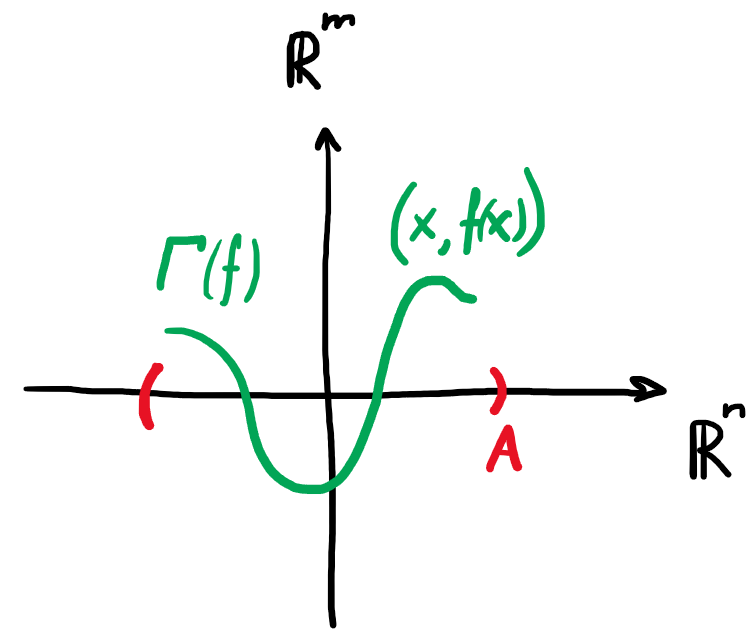
\includegraphics[width=0.5\textwidth,keepaspectratio]{img7}
\end{figure}

Si può dotare $ \Gamma(f) $ di una struttura di varietà differenziabile di dimensione $ n $.\\
Il grafico $ \Gamma(f) \subset \R^{n+m} $ è $ N_{2}+T_{2} $ (perché lo è $ \R^{n+m} $) dunque è una varietà topologica. Considerando l'applicazione

\map{\phi}%
	{\Gamma(f)}{A}%
	{(x,f(x))}{x}

possiamo costruire un'unica carta $ (\Gamma(f),\phi) $ con $ \phi $ omeomorfismo, la quale comporta l'esistenza di un atlante massimale che la contenga. L'applicazione $ \phi $ è un omeomorfismo perché è continua e la sua inversa è continua perché $ f $ è liscia.

\paragraph{6. Gruppo lineare}

Sia l'insieme

\begin{equation}
	GL_{n}(\R) = \{ A \in M_{n}(\R) \mid \det A \neq 0 \} \subset M_{n}(\R)
\end{equation}

Si può identificare l'insieme delle matrici quadrate con lo spazio euclideo $ M_{n}(\R) = \R^{n^{2}} $ (mappando le righe delle matrici in ordine per creare un vettore di $ n^{2} $ componenti).\\
Con la topologia indotta da $ \R^{n^{2}} $, lo spazio $ GL_{n}(\R) $ è $ N_{2}+T_{2} $. Inoltre, $ GL_{n}(\R) $ è un aperto di $ M_{n}(\R) $ perché è il complementare dell'insieme chiuso

\begin{equation}
	 M_{n}(\R) \setminus GL_{n}(\R) = \{ A \in M_{n}(\R) \mid \det A = 0 \}
\end{equation}

in quanto il determinante è un'applicazione continua e la controimmagine di $ 0 $ è un chiuso.\\
Essendo quindi un aperto di una varietà, $ GL_{n}(\R) $ è una varietà differenziabile con l'unica carta $ \id $; questa varietà ha $ \dim(GL_{n}(\R)) = n^{2} $.

\paragraph{7. Cerchio unitario $ \S^{1} $}\label{ex-s1}

Il cerchio unitario $ \S^{1} $

\begin{equation}
	\S^{1} = \left\{ (x,y) \in \R^{2} \, \middle| \, x^{2} + y^{2} = 1 \right\}
\end{equation}

con la topologia indotta da $ \R^{2} $ (quindi è $ N_{2}+T_{2} $) può essere dotato di una struttura differenziabile costituita da 4 carte prendendo gli aperti\footnote{%
	Questi insiemi sono aperti perché intersezioni di $ \S^{1} $ aperto con aperti di $ \R^{n} $, e.g. il semipiano superiore.}

\begin{align}
	\begin{split}
		U_{1} &= \left\{ (x,y) \in \S^{1} \, \middle| \, y>0 \right\}\\
		U_{2} &= \left\{ (x,y) \in \S^{1} \, \middle| \, y<0 \right\}\\
		U_{3} &= \left\{ (x,y) \in \S^{1} \, \middle| \, x>0 \right\}\\
		U_{4} &= \left\{ (x,y) \in \S^{1} \, \middle| \, x<0 \right\}
	\end{split}	
\end{align}

i quali sono un ricoprimento del cerchio unitario, i.e.

\begin{equation}
	\S^{1} = \bigcup_{k=1}^{4} U_{k}
\end{equation}

Definiamo ora 4 funzioni che costituiranno, insieme agli aperti sopra definiti, un atlante per lo spazio

\begin{align}
	\begin{split}
		\phi_{1} : U_{1} &\to (-1,1)_{x} \in \R^{2}\\
		(x,y) &\mapsto x\\\\
		%
		\phi_{2} : U_{2} &\to (-1,1)_{x} \in \R^{2}\\
		(x,y) &\mapsto x\\\\
		%
		\phi_{3} : U_{3} &\to (-1,1)_{y} \in \R^{2}\\
		(x,y) &\mapsto y\\\\
		%
		\phi_{4} : U_{4} &\to (-1,1)_{y} \in \R^{2}\\
		(x,y) &\mapsto y
	\end{split}
\end{align}

\begin{figure}[H]
\centering
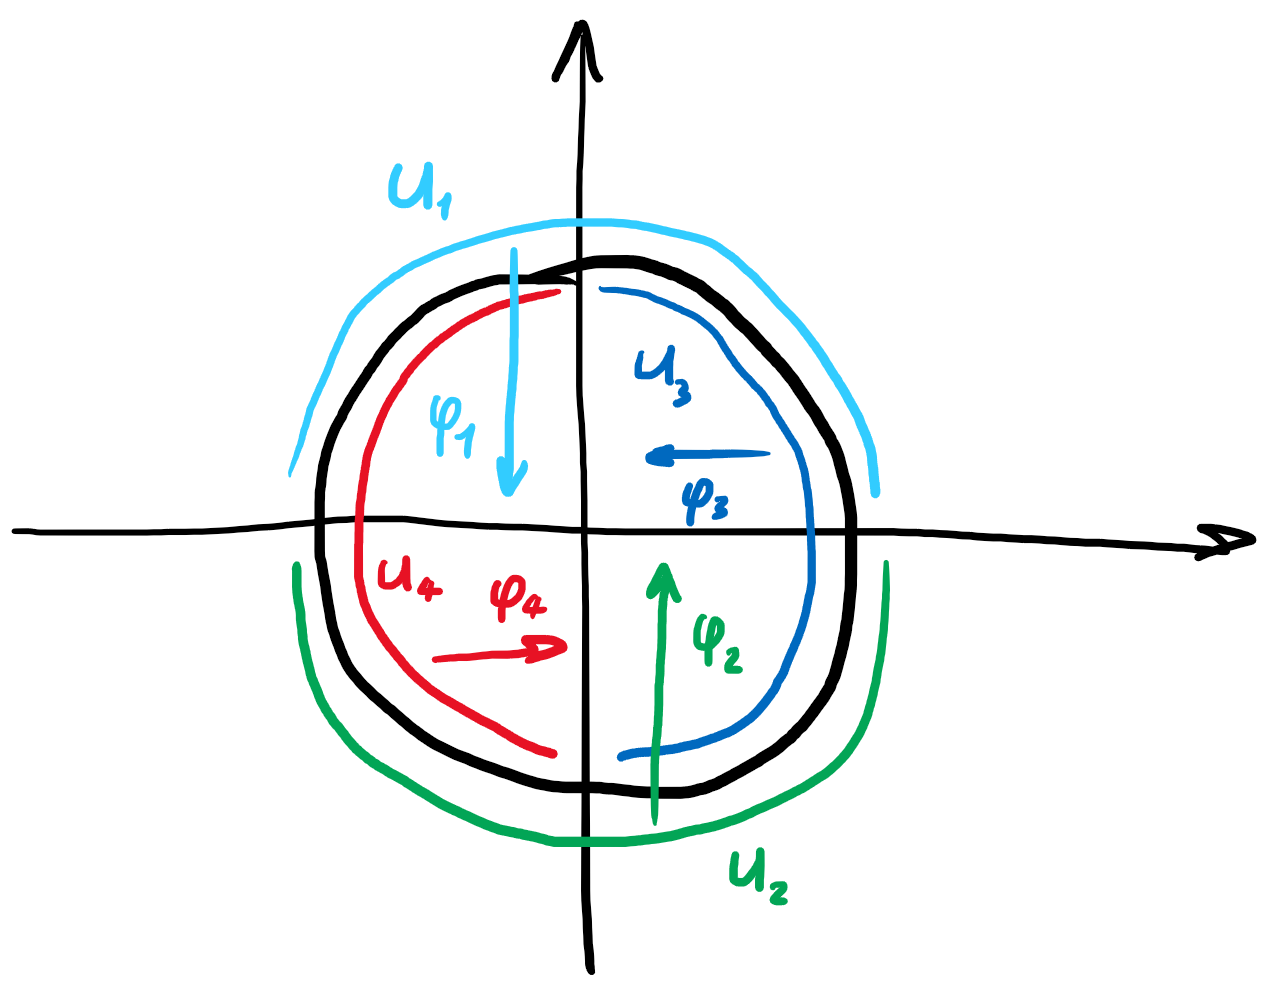
\includegraphics[width=0.5\textwidth,keepaspectratio]{img8}
\end{figure}

Vogliamo mostrare che $ \{(U_{i},\phi_{i})\}_{i=1,\dots,4} $ sia un atlante differenziabile in modo tale da dotare $ \S^{1} $ di un atlante massimale e quindi renderlo una varietà differenziabile.\\
Dimostriamo prima che le $ \phi_{i} $ siano omeomorfismi: sono continue e lisce perché sono restrizioni ad una delle componenti e le inverse

\begin{align}
	\begin{split}
		\phi_{1}^{-1} : (-1,1)_{x} &\to U_{1}\\
		x &\mapsto (x,\sqrt{1-x^{2}})\\\\
		%
		\phi_{2}^{-1} : (-1,1)_{x} &\to U_{2}\\
		x &\mapsto (x,-\sqrt{1-x^{2}})\\\\
		%
		\phi_{3}^{-1} : (-1,1)_{y} &\to U_{3}\\
		y &\mapsto (\sqrt{1-y^{2}},y)\\\\
		%
		\phi_{4}^{-1} : (-1,1)_{y} &\to U_{4}\\
		y &\mapsto (-\sqrt{1-y^{2}},y)
	\end{split}
\end{align}

sono anch'esse continue e lisce; questo dimostra che lo spazio è una varietà topologica.\\
Per dimostrare che sia una struttura differenziabile, prendiamo due carte arbitrarie e ne facciamo la composizione per controllare la loro $ C^{\infty} $-compatibilità:

\begin{align}
	\begin{split}
		\phi_{3} \circ \phi_{1}^{-1} : \phi_{1}(U_{1} \cap U_{3}) &\to \phi_{3}(U_{1} \cap U_{3})\\
		\phi_{1} \circ \phi_{3}^{-1} : \phi_{3}(U_{1} \cap U_{3}) &\to \phi_{1}(U_{1} \cap U_{3})
	\end{split}
\end{align}

dove

\begin{equation}
	U_{1} \cap U_{3} = \left\{ (x,y) \in \S^{1} \, \middle| \, x>0 \, \wedge \, y>0  \right\}
\end{equation}

e dunque

\begin{align}
	\begin{split}
		\phi_{1}(U_{1} \cap U_{3}) &= (0,1)_{x}\\
		\phi_{3}(U_{1} \cap U_{3}) &= (0,1)_{y}
	\end{split}
\end{align}

L'azione delle composizioni è la seguente

\begin{align}
	\begin{split}
		(\phi_{3} \circ \phi_{1}^{-1}) (x) &= \phi_{3} ((x,\sqrt{1-x^{2}}))\\
		&= \sqrt{1-x^{2}}\\\\
		%
		(\phi_{1} \circ \phi_{3}^{-1}) (y) &= \phi_{1} ((\sqrt{1-y^{2}},y))\\
		&= \sqrt{1-y^{2}}
	\end{split}
\end{align}

Queste applicazioni sono lisce in quanto le loro derivate non divergono mai perché i denominatori non si annullano mai negli intervalli dei domini.\\
Il ragionamento è analogo per tutte le altre composizioni, dunque $ \{(U_{i},\phi_{i})\}_{i=1,\dots,4} $ è un atlante differenziabile per $ \S^{1} $.

\paragraph{8. Sfera unitaria $ \S^{2} $}

La sfera unitaria $ \S^{2} $ è una varietà topologica inclusa in $ \R^{3} $ (che induce la topologia e le proprietà di $ N_{2}+T_{2} $).\\
Gli aperti che ricoprono lo spazio sono i seguenti

\begin{align}
	\begin{split}
		U_{1} &= \left\{ (x,y,z) \in \S^{2} \, \middle| \, z>0 \right\}\\
		U_{2} &= \left\{ (x,y,z) \in \S^{2} \, \middle| \, z<0 \right\}\\
		U_{3} &= \left\{ (x,y,z) \in \S^{2} \, \middle| \, y>0 \right\}\\
		U_{4} &= \left\{ (x,y,z) \in \S^{2} \, \middle| \, y<0 \right\}\\
		U_{5} &= \left\{ (x,y,z) \in \S^{2} \, \middle| \, x>0 \right\}\\
		U_{6} &= \left\{ (x,y,z) \in \S^{2} \, \middle| \, x<0 \right\}
	\end{split}	
\end{align}

Prendendo il generico aperto

\begin{equation}
	D_{ij} \doteq \left\{ (i,j) \in \R^{2} \, \middle| \, i^{2}+j^{2}<1 \right\}
\end{equation}

definiamo dunque le applicazioni

\begin{align}
	\begin{split}
		\phi_{1} : U_{1} &\to D_{xy} \in \R^{2}\\
		(x,y,z) &\mapsto (x,y)\\\\
		%
		\phi_{2} : U_{2} &\to D_{xy} \in \R^{2}\\
		(x,y,z) &\mapsto (x,y)\\\\
		%
		\phi_{3} : U_{3} &\to D_{xz} \in \R^{2}\\
		(x,y,z) &\mapsto (x,z)\\\\
		%
		\phi_{4} : U_{4} &\to D_{xz} \in \R^{2}\\
		(x,y,z) &\mapsto (x,z)\\\\
		%
		\phi_{5} : U_{5} &\to D_{yz} \in \R^{2}\\
		(x,y,z) &\mapsto (y,z)\\\\
		%
		\phi_{6} : U_{6} &\to D_{yz} \in \R^{2}\\
		(x,y,z) &\mapsto (y,z)
	\end{split}
\end{align}

per formare le carte $ \{(U_{i},\phi_{i})\}_{i=1,\dots,6} $.

\begin{figure}[H]
	\centering
	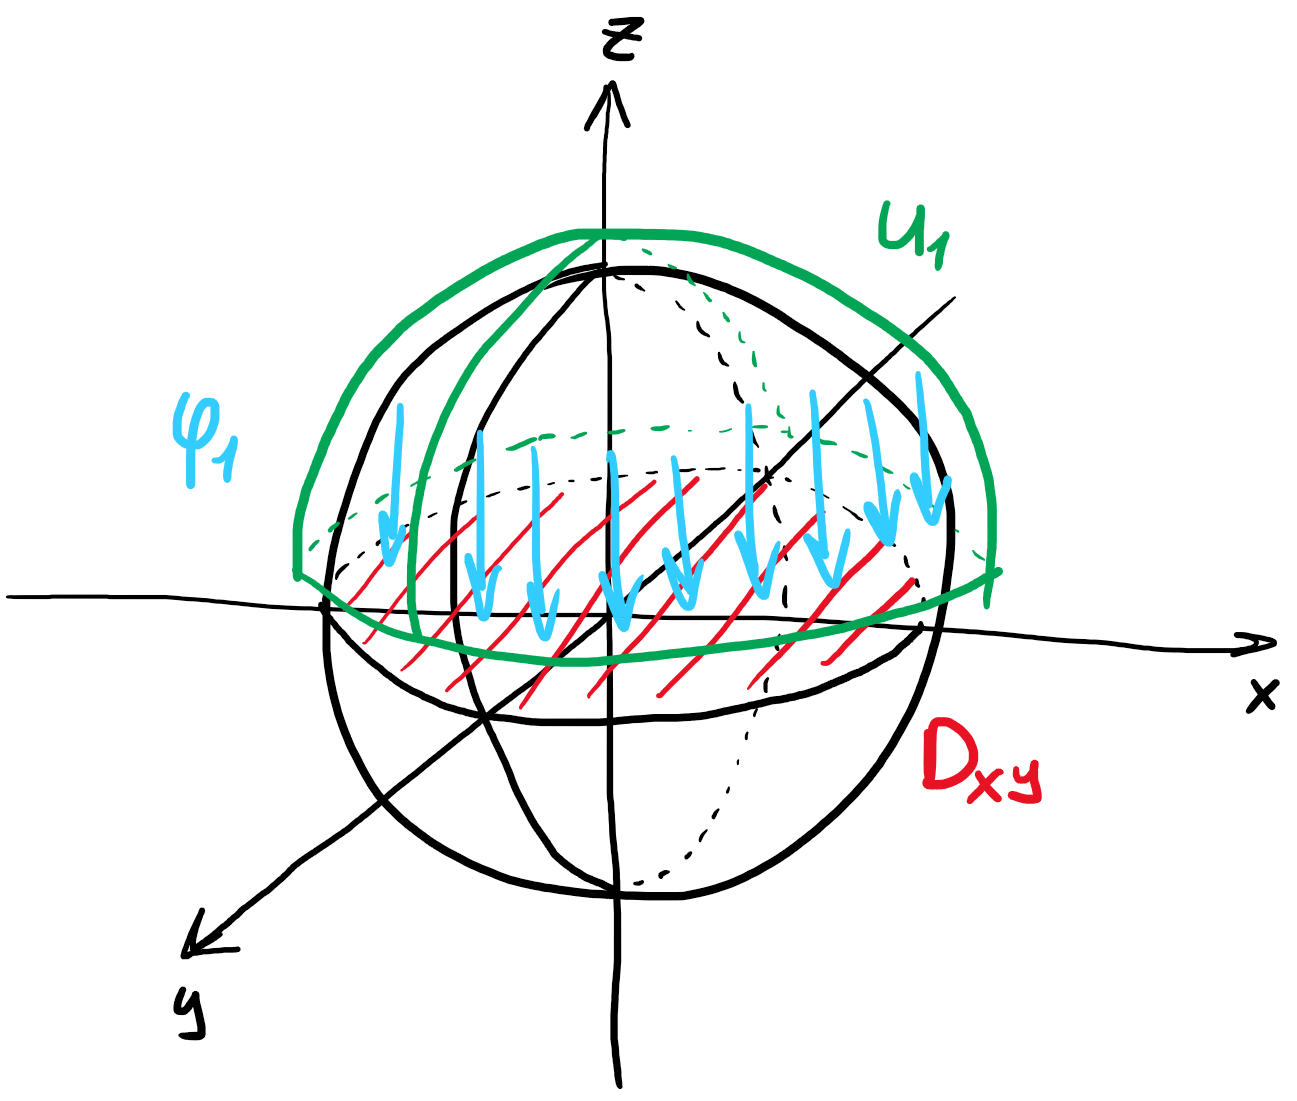
\includegraphics[width=0.7\textwidth,keepaspectratio]{img9}
\end{figure}

Le applicazioni inverse sono

\begin{align}
	\begin{split}
		\phi_{1}^{-1} : D_{xy} &\to U_{1} \in \R^{2}\\
		(x,y) &\mapsto (x,y,\sqrt{1-x^{2}-y^{2}})\\\\
		%
		\phi_{2}^{-1} : D_{xy} &\to U_{2} \in \R^{2}\\
		(x,y) &\mapsto (x,y,-\sqrt{1-x^{2}-y^{2}})\\\\
		%
		\phi_{3}^{-1} : D_{xz} &\to U_{3} \in \R^{2}\\
		(x,z) &\mapsto (x,\sqrt{1-x^{2}-z^{2}},z)\\\\
		%
		\phi_{4}^{-1} : D_{xz} &\to U_{4} \in \R^{2}\\
		(x,z) &\mapsto (x,-\sqrt{1-x^{2}-z^{2}},z)\\\\
		%
		\phi_{5}^{-1} : D_{yz} &\to U_{5} \in \R^{2}\\
		(y,z) &\mapsto (\sqrt{1-y^{2}-z^{2}},y,z)\\\\
		%
		\phi_{6}^{-1} : D_{yz} &\to U_{6} \in \R^{2}\\
		(y,z) &\mapsto (-\sqrt{1-y^{2}-z^{2}},y,z)
	\end{split}
\end{align}

Ad esempio, verifichiamo che le carte $ (U_{1},\phi_{1}) $ e $ (U_{4},\phi_{4}) $ siano compatibili:

\begin{align}
	\begin{split}
		\phi_{1} \circ \phi_{4}^{-1} : \phi_{4}(U_{1} \cap U_{4}) &\to \phi_{1}(U_{1} \cap U_{4})\\
		\phi_{4} \circ \phi_{1}^{-1} : \phi_{1}(U_{1} \cap U_{4}) &\to \phi_{4}(U_{1} \cap U_{4})
	\end{split}
\end{align}

dove $ U_{1} \cap U_{4} = \left\{ (x,y,z) \in \S^{2} \, \middle| \, z>0 \, \wedge \, y<0 \right\} $ e dunque 

\begin{align}
	\begin{split}
		(\phi_{1} \circ \phi_{4}^{-1})(x,z) &= \phi_{1} \left( x,-\sqrt{1-x^{2}-z^{2}},z \right)\\
		&= \left( x,-\sqrt{1-x^{2}-z^{2}} \right)\\\\
		%
		(\phi_{4} \circ \phi_{1}^{-1})(x,y) &= \phi_{4} \left( x,y,\sqrt{1-x^{2}-y^{2}} \right)\\
		&= \left( x,\sqrt{1-x^{2}-y^{2}} \right)
	\end{split}
\end{align}

e analogamente per le altre composizioni. Tutte queste applicazioni e le loro inverse sono lisce per lo stesso motivo dato per il cerchio unitario.\\
Tutto ciò dota lo spazio di un atlante differenziabile e dunque la sfera unitaria $ \S^{2} $ di una struttura differenziabile.\\
Vedi Esercizio \ref{es2-1}.

\paragraph{9. Sfera unitaria $ \S^{n} $ con proiezione stereografica}

La sfera unitaria $ \S^{n} $ è l'insieme

\begin{equation}
	\S^{n} = \left\{ x = (x^{1},\dots,x^{n}) \in \R^{n} \, \middle| \, \norm{x} \doteq \sum_{i=1}^{n} (x^{i})^{2} = 1 \right\}
\end{equation}

ha la topologia indotta da $ \R^{n+1} $ (quindi è $ N_{2}+T_{2} $).\\
Siano i poli $ N = (0,\dots,0,1) $ e $ S = (0,\dots,0,-1) $ da cui i due aperti\footnote{%
	Sono aperti perché complementari di un chiuso, i.e. i punti ai poli.%
} per le carte

\begin{align}
	\begin{split}
		U_{N} &= \S^{n} \setminus \{N\}\\
		U_{S} &= \S^{n} \setminus \{S\}
	\end{split}
\end{align}

Costruiamo ora le applicazioni per la proiezione stereografica

\begin{align}
	\begin{split}
		\pi_{N} : \S^{n} \setminus \{N\} &\to \R^{n} \times \{0\} = \R^{n}\\
		(x^{1},\dots,x^{n+1}) &\mapsto \left( \dfrac{2x^{1}}{1-x^{n+1}},\dots,\dfrac{2x^{n}}{1-x^{n+1}} \right)\\\\
		%
		\pi_{S} : \S^{n} \setminus \{S\} &\to \R^{n} \times \{0\} = \R^{n}\\
		(x^{1},\dots,x^{n+1}) &\mapsto \left( \dfrac{2x^{1}}{1+x^{n+1}},\dots,\dfrac{2x^{n}}{1+x^{n+1}} \right)
	\end{split}
\end{align}

Queste applicazioni si ottengono considerando una retta per uno dei poli e il punto da proiettare e l'intersezione della retta stessa con il piano $ \R^{n} \times \{0\} = \R^{n} $.

\begin{figure}[H]
	\centering
	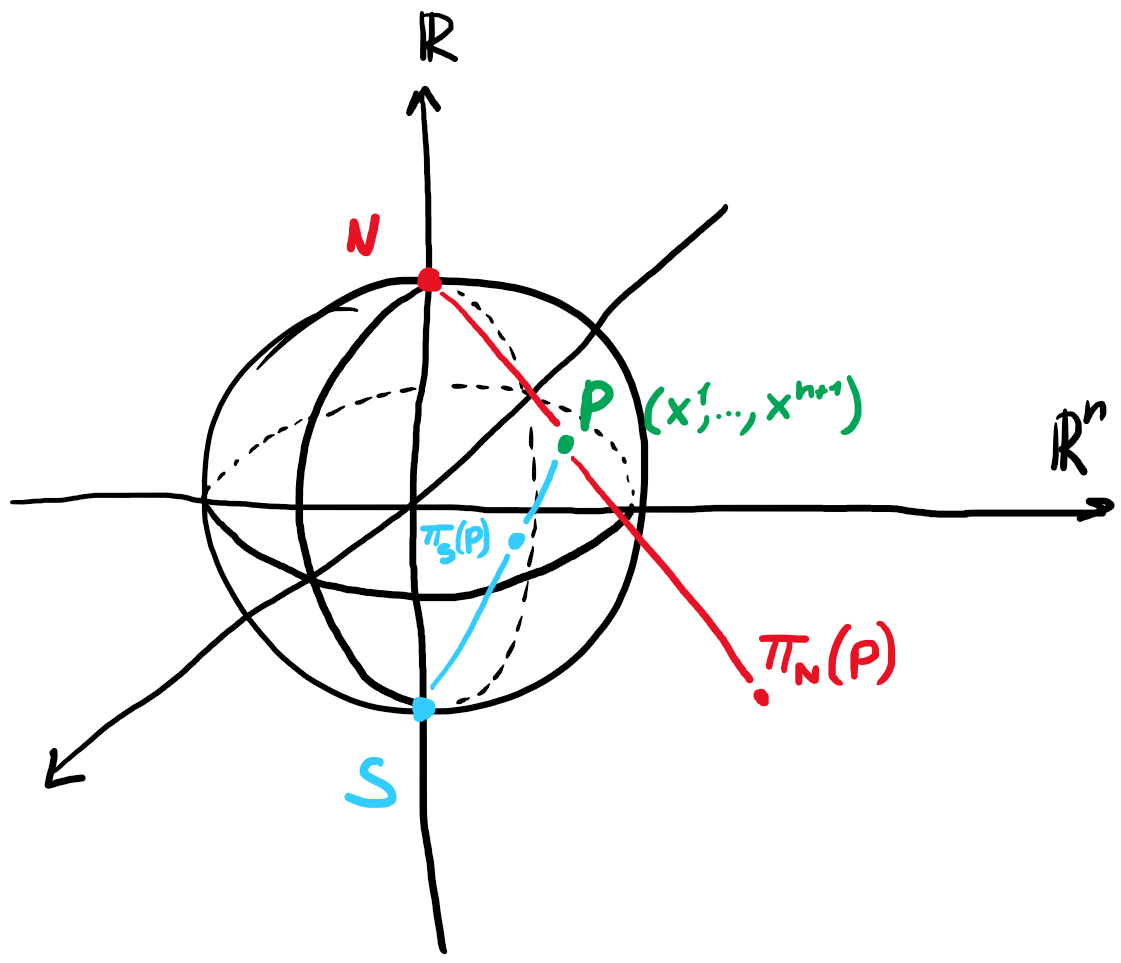
\includegraphics[width=0.6\textwidth,keepaspectratio]{img10}
\end{figure}

Le inverse delle applicazioni sono

\begin{align}
	\begin{split}
		\pi_{N}^{-1} : \R^{n} &\to \S^{n} \setminus \{N\}\\
		(x^{1},\dots,x^{n}) &\mapsto \left( \dfrac{x^{1}}{1+\norm{x}^{2}},\dots,\dfrac{x^{n}}{1+\norm{x}^{2}},\dfrac{\norm{x}^{2}-1}{1+\norm{x}^{2}} \right)\\\\
		%
		\pi_{S}^{-1} : \R^{n} &\to \S^{n} \setminus \{S\}\\
		(x^{1},\dots,x^{n}) &\mapsto \left( \dfrac{x^{1}}{1+\norm{x}^{2}},\dots,\dfrac{x^{n}}{1+\norm{x}^{2}},\dfrac{1-\norm{x}^{2}}{1+\norm{x}^{2}} \right)
	\end{split}
\end{align}

Sia le funzioni che le loro inverse sono lisce e sono omeomorfismi.\\
Per dotare $ \S^{n} $ di una struttura differenziabile prendendo l'atlante massimale che include queste due carte, è necessario verificare che i cambi di carte siano lisci

\begin{align}
	\begin{split}
		\pi_{N} \circ \pi_{S}^{-1} : \pi_{S}(U_{S} \cap U_{N}) &\to \pi_{N}(U_{S} \cap U_{N})\\
		\pi_{S} \circ \pi_{N}^{-1} : \pi_{N}(U_{S} \cap U_{N}) &\to \pi_{S}(U_{S} \cap U_{N})
	\end{split}
\end{align}

dove $ U_{S} \cap U_{N} = \S^{n} \setminus \{N,S\} $ e quindi $ \pi_{S}(U_{S} \cap U_{N}) = \pi_{N}(U_{S} \cap U_{N}) = \R^{n} \setminus \{0\} $, perciò

\begin{align}
	\begin{split}
		\pi_{N} \circ \pi_{S}^{-1} : \R^{n} \setminus \{0\} &\to \R^{n} \setminus \{0\}\\
		(x^{1},\dots,x^{n}) &\mapsto \pi_{N}\left( \dfrac{x^{1}}{1+\norm{x}^{2}},\dots,\dfrac{x^{n}}{1+\norm{x}^{2}},\dfrac{1-\norm{x}^{2}}{1+\norm{x}^{2}} \right) =\\
		&= (x^{1},\dots,x^{n})
	\end{split}
\end{align}

e la sua inversa è identica a sé stessa $ \pi_{S} \circ \pi_{N}^{-1} \equiv \pi_{N} \circ \pi_{S}^{-1} $; queste composizioni sono lisce dunque le carte $ (U_{N},\pi_{N}) $ e $ (U_{S},\pi_{S}) $ sono $ C^{\infty} $-compatibili perciò $ \{(U_{N},\pi_{N}),(U_{S},\pi_{S})\} $ è un atlante differenziabile su $ \S^{n} $, il quale diventa una varietà differenziabile.\\
Vedi Esercizio \ref{es2-2}.

\paragraph{10. Prodotto di varietà differenziabili}

Prendiamo due varietà differenziabili $ M $ ed $ N $ e consideriamo il prodotto cartesiano $ M \times N $ con \textit{topologia prodotto}, il che rende $ M \times N $ ancora $ N_{2}+T_{2} $.\\
Siano $ \mathfrak{U} = \{(U_{\alpha},\phi_{\alpha})\}_{\alpha \in A} $ un atlante differenziabile di $ M $ e $ \mathfrak{V} = \{(V_{\beta},\psi_{\beta})\}_{\beta \in B} $ un atlante differenziabile di $ N $.\\
Sia un atlante per $ M \times N $

\begin{equation}
	\mathfrak{W} = \{(U_{\alpha} \times V_{\beta},\phi_{\alpha} \times \psi_{\beta})\}_{\alpha \in A, \, \beta \in B}
\end{equation}

dove al variare di $ \alpha $ e $ \beta $ per l'aperto $ U_{\alpha} \times V_{\beta} \in M \times N $ si ottiene un ricoprimento per lo spazio prodotto, i.e.

\begin{equation}
	M \times N = \bigcup_{\alpha,\beta} (U_{\alpha} \times V_{\beta})
\end{equation}

Le applicazioni

\begin{align}
	\begin{split}
		\phi_{\alpha} \times \psi_{\beta} : U_{\alpha} \times V_{\beta} &\to \phi_{\alpha}(U_{\alpha}) \times \psi_{\beta}(V_{\beta}) \subset \R^{m} \times \R^{n} = \R^{m+n}\\
		(x,y) &\mapsto (\phi_{\alpha}(x),\psi_{\beta}(y))
	\end{split}
\end{align}

dove $ \dim M = m $ e $ \dim N = n $, sono continue (il prodotto di applicazioni continue è continuo) perché omeomorfismi e le inverse sono il prodotto delle inverse

\begin{equation}
	(\phi_{\alpha} \times \psi_{\beta})^{-1} = \phi_{\alpha}^{-1} \times \psi_{\beta}^{-1} : \phi_{\alpha}(U_{\alpha}) \times \psi_{\beta}(V_{\beta}) \to U_{\alpha} \times V_{\beta}
\end{equation}

anch'esse continue perché inverse di omeomorfismi.\\
Questo rende $ \mathfrak{W} $ un atlante topologico; perché sia un atlante differenziabile, verifichiamo che le carte siano $ C^{\infty} $-compatibili controllando che i cambi di carte siano omeomorfismi

\begin{equation}
	(\phi_{\alpha} \times \psi_{\beta}) \circ (\phi_{\rho} \times \psi_{\sigma})^{-1} : (\phi_{\rho} \times \psi_{\sigma})(U_{\rho} \times V_{\sigma}) \to (\phi_{\alpha} \times \psi_{\beta})(U_{\alpha} \times V_{\beta})
\end{equation}

alternativamente

\begin{equation}
	(\phi_{\alpha} \circ \phi_{\rho}^{-1}) \times (\psi_{\beta} \circ \psi_{\sigma})^{-1} : \phi_{\rho}(U_{\rho}) \times \psi_{\sigma}(V_{\sigma}) \to \phi_{\alpha}(U_{\alpha}) \times \psi_{\beta}(V_{\beta})
\end{equation}

le composizioni $ \phi_{\alpha} \circ \phi_{\rho}^{-1} $ e $ \psi_{\beta} \circ \psi_{\sigma} $ sono lisce perché ognuna di queste prova la compatibilità delle carte in $ M $ e in $ N $ rispettivamente e dunque il loro prodotto è ancora liscio. Questi ragionamenti portano all'esistenza di una struttura differenziale per $ M \times N $ il quale diventa una varietà differenziabile.\\
La dimensione del prodotto di varietà è $ \dim (M \times N) = \dim M + \dim N $.\\
Il toro bidimensionale $ \T^{2} = \S^{1} \times \S^{1} $ e il cilindro infinito $ \mathcal{C} = \S^{1} \times \R $ sono superfici differenziabili; anche il toro $ n $-dimensionale è una varietà differenziabile

\begin{align}
	\T^{n} = \prod^{n} \S^{1}
\end{align}

dove la produttoria implica la topologia prodotto $ \times $.

\subsection{Spazi quoziente dal punto di vista topologico}

Sia $ S $ uno spazio topologico e $ \sim $ una relazione di equivalenza su $ S $. Dalla relazione di equivalenza deriva una proiezione sullo \textit{spazio quoziente} $ \sfrac{S}{\sim} $, mappando un elemento $ x \in S $ nella classe di equivalenza $ [x] $, i.e.

\begin{align}
	\begin{split}
		\pi : S &\to \sfrac{S}{\sim}\\
		x &\mapsto [x]
	\end{split}
\end{align}

Definiamo una topologia su $ \sfrac{S}{\sim} $ definendo un insieme $ U $ tale che

\begin{equation}
	U \text{ aperto in } \sfrac{S}{\sim} \iff U = \{\} \, \wedge \, U = \sfrac{S}{\sim} \, \wedge \, \pi^{-1}(U) \text{ aperto in } S
\end{equation}

cioè $ U $ è aperto se e solo se la sua controimmagine è aperta in $ S $.\\
Per verificare che questa sia una topologia è necessario che l'intersezione di due aperti e l'unione arbitraria di aperti siano ancora aperti: queste proprietà sono soddisfatte perché rispettate da $ \pi^{-1} $

\begin{align}
	\begin{split}
		\pi^{-1}(U \cap V) &= \pi^{-1}(U) \cap \pi^{-1}(V)\\
		\pi^{-1}\left( \bigcup_{j \in J} V_{j} \right) &= \bigcup_{j \in J} \pi^{-1}(V_{j})
	\end{split}
\end{align}

Questa topologia è chiamata \textit{topologia quoziente} su $ \sfrac{S}{\sim} $.

\begin{remark}
	Una volta fissata la topologia quoziente, la proiezione $ \pi : S \to \sfrac{S}{\sim} $ è continua, perché la controimmagine di un aperto è aperta\footnote{%
		Un insieme è aperto se e solo se la sua controimmagine è aperta.%
	}.
\end{remark}

Definiamo l'applicazione $ f : S \to Y $ con $ S $ e $ Y $ spazi topologici: questa applicazione è \textit{costante sulle classi di equivalenza} se, presi due elementi $ s_{1},s_{2} \in S $, si ha che

\begin{equation}
	s_{1} \sim s_{2} \implies f(s_{1}) = f(s_{2})
\end{equation}

Questa proprietà permette di considerare una seconda applicazione

\begin{align}
	\begin{split}
		\tilde{f} : \sfrac{S}{\sim} &\to Y\\
		[s] &\mapsto f(s)
	\end{split}
\end{align}

la quale è ben definita in quanto non importi il rappresentante della classe $ [s] $ al fine del calcolo di $ f(s) $.\\
Una proprietà di queste applicazioni è la seguente

\begin{equation}
	f = \tilde{f} \circ \pi
\end{equation}

come si può evincere dal seguente diagramma

\begin{figure}[H]
	\centering
	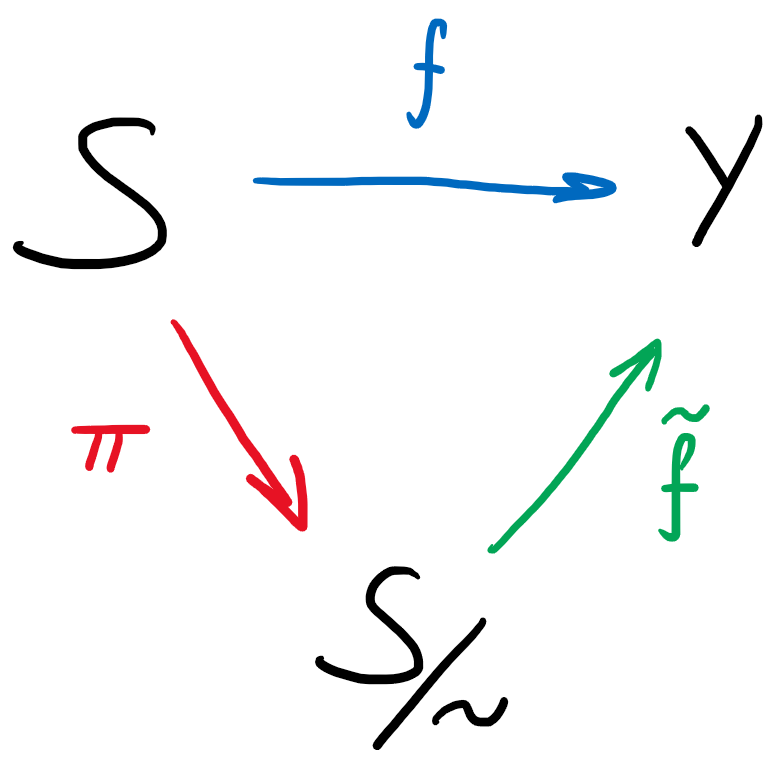
\includegraphics[width=0.2\textwidth,keepaspectratio]{img11}
\end{figure}

\begin{definition}
	$ f $ è continua $ \iff $ $ \tilde{f} $ è continua
\end{definition}

\begin{proof}[Dimostrazione ($ \impliedby $)]
	Se $ \tilde{f} $ è continua, siccome lo è anche $ \pi $, la composizione di funzioni continue è continua dunque $ f = \tilde{f} \circ \pi $ è continua.
\end{proof}

\begin{proof}[Dimostrazione ($ \implies $)]
	Sia $ V $ un aperto di $ Y $: prendiamo la controimmagine di $ V $ tramite la funzione continua $ f $
	
	\begin{align}
		\begin{split}
			f^{-1}(V) &= (\tilde{f} \circ \pi)^{-1}(V)\\
			&= \pi^{-1}(\tilde{f}^{-1}(V))
		\end{split}
	\end{align}

	Siccome $ f $ è continua, $ f^{-1}(V) $ è aperto dunque anche $ \pi^{-1}(\tilde{f}^{-1}(V)) $ è aperto: per definizione di topologia quoziente anche $ \tilde{f}^{-1}(V) $ è aperto in $ S $. Quest'ultima è la definizione di applicazione continua dunque $ \tilde{f} $ è continua.
\end{proof}

\subsubsection{\textit{Esempi}}

\paragraph{1.}

Sia $ S $ uno spazio topologico e $ A $ un suo qualsiasi sottoinsieme. Definiamo la relazione di equivalenza $ \sim $ su $ S $ come

\begin{equation}
	\begin{cases}
		x \sim x & \qq*{se} x \in S \setminus A\\
		x \sim y & \qq*{se} x,y \in A
	\end{cases}
\end{equation}

cioè ogni punto di $ S \setminus A $ è identificato con sé stesso mentre tutti i punti di $ A $ sono identificati tra loro\footnote{%
	Tutti i punti di $ S \setminus A $ vanno in sé stessi mentre tutti i punti di $ A $ vanno in uno solo.%
}.\\
Scriviamo lo spazio quoziente rispetto a questa relazione di equivalenza come $ \sfrac{S}{\sim} = \sfrac{S}{A} $, chiamato \textit{spazio ottenuto da} $ S $ \textit{tramite} $ A $.

\paragraph{2.}

Sia $ S = I = [0,1] $ e $ A = \{0,1\} $ e consideriamo $ \sfrac{S}{A} = \sfrac{I}{\{0,1\}} $: utilizzando la stessa relazione di equivalenza $ \sim $ dell'esempio precedente si può identificare lo spazio quoziente $ \sfrac{I}{\{0,1\}} $ come un cerchio, in quanto tutti i punti di $ I $ vengono identificati con sé stessi mentre gli estremi $ A = \{0,1\} $ si identificano uno con l'altro.\\
Si dimostra l'omeomorfismo $ \sfrac{I}{\{0,1\}} \simeq \S^{1} $.

\begin{figure}[H]
	\centering
	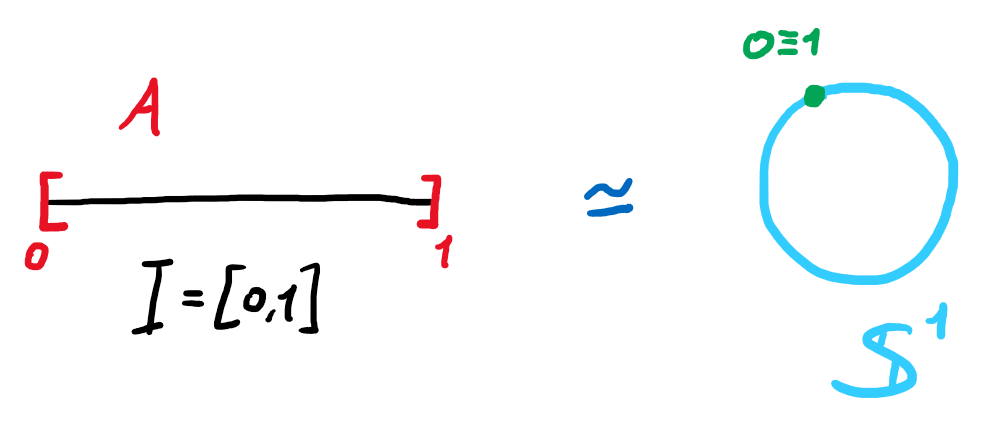
\includegraphics[width=0.6\textwidth,keepaspectratio]{img12}
\end{figure}

Sia l'applicazione

\map{f}%
	{I}{\S^{1}}%
	{x}{e^{2 i \pi x} = (\cos(2 \pi x), \sin(2 \pi x))}

questa è continua e costante sulle classi di equivalenza di $ \sfrac{I}{\{0,1\}} $. A questo punto è possibile costruire il diagramma

\begin{figure}[H]
	\centering
	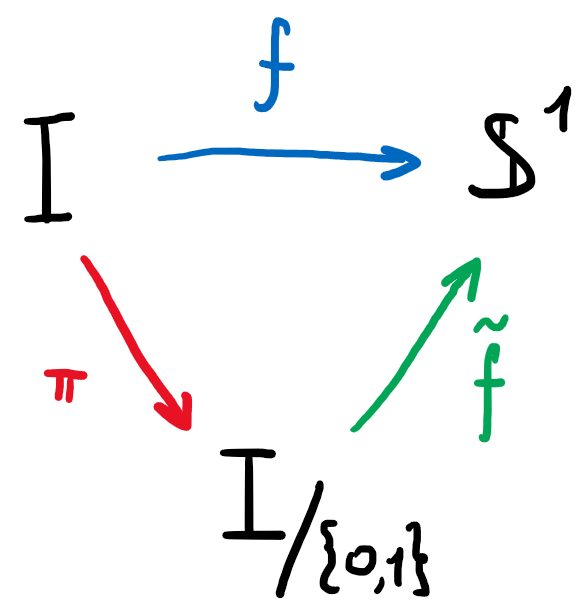
\includegraphics[width=0.2\textwidth,keepaspectratio]{img13}
\end{figure}

il quale implica l'esistenza di una funzione $ \tilde{f} $ la quale è continua perché $ f $ è continua.\\
L'applicazione $ \tilde{f} $ è anche iniettiva e suriettiva: perché sia identificato come un omeomorfismo, si utilizza il seguente lemma

\begin{lemma}[dell'applicazione chiusa]\label{lemma-clos-app}
	Se si ha una bigezione continua da uno spazio compatto ad uno spazio $ T_{2} $ o di Hausdorff, allora questa è un omeomorfismo.
\end{lemma}

dove $ \sfrac{I}{\{0,1\}} $ è uno spazio compatto perché quoziente dello spazio compatto $ I $, cioè immagine di un compatto tramite un'applicazione continua e $ \S^{1} $ è $ T_{2} $ o di Hausdorff perché incluso in $ \R^{2} $.

\begin{proof}[Dimostrazione (Lemma dell'applicazione chiusa)]
	\`{E} sufficiente far vedere che l'applicazione sia chiusa: lo è perché un chiuso in un compatto è compatto, l'immagine di un compatto tramite un'applicazione continua è un compatto e un sottoinsieme compatto di uno spazio di Hausdorff è chiuso.
\end{proof}

\paragraph{3.}

Sia $ S = \R $ e $ A = (0,+\infty) $ e consideriamo $ \sfrac{S}{A} = \sfrac{\R}{A} $. Lo spazio quoziente non è di Hausdorff perché, se lo fosse, ogni suo punto sarebbe un chiuso cioè $ \sfrac{\R}{A} $ sarebbe\footnote{%
	Per un qualsiasi insieme $ E $, se questo è $ T_{2} $ o di Hausdorff allora è $ T_{1} $ e anche $ T_{0} $, i.e. $ T_{2} \implies T_{1} \implies T_{0} $.%
} $ T_{1} $.\\
Considerando la classe di equivalenza $ [A] \in \sfrac{\R}{A} $, questa è chiusa se la sua controimmagine è chiusa ma

\begin{equation}
	\pi^{-1} ([A]) = (0,+\infty)
\end{equation}

il quale è un aperto perciò $ [A] $ non è chiuso e lo spazio quoziente non è di Hausdorff.

\paragraph{4.}

Sia $ S = \R $ e $ A = \Q $. Si dimostra che $ \sfrac{\R}{\Q} $ non è $ N_{2} $ e nemmeno $ N_{1} $.

\subsubsection{Relazione di equivalenza aperta}

Sia $ S $ uno spazio topologico e $ \sim $ una relazione di equivalenza su $ S $. Diremo che $ \sim $ è aperta se l'applicazione sul quoziente $ \pi : S \to \sfrac{S}{\sim} $ è aperta.

\subsubsection{\textit{Esempio}}

Sia $ S = \R $ e $ A = \{-1,1\} $ e consideriamo $ \sfrac{S}{A} = \sfrac{\R}{\{-1,1\}} $.\\
L'applicazione $ \pi : \R \to \sfrac{\R}{\{-1,1\}} $ non è aperta perché, per esempio $ \pi((0,2)) $ non è aperto in $ \sfrac{\R}{\{-1,1\}} $ perché la sua controimmagine è pari a

\begin{equation}
	\pi^{-1}(\pi((0,2))) = (0,2) \cup \{-1\}
\end{equation}

in quanto i punti $ \{-1,1\} $ sono equivalenti, ma questo insieme non è aperto in $ \R $.

\subsubsection{Proprietà $ N_{2} $ e $ T_{2} $ dei quozienti}

\begin{definition}\label{prop-n2}
	Se lo spazio topologico $ S $ è $ N_{2} $ e la relazione di equivalenza $ \sim $ è aperta allora il quoziente $ \sfrac{S}{\sim} $ è $ N_{2} $.
\end{definition}

\begin{proof}\label{solved-es2-4}
	Per dimostrare questa proposizione è necessario costruire una base numerabile per $ \sfrac{S}{\sim} $ sapendo che ne esiste una in $ S $.\\
	Sia $ \{B_{n}\}_{n \in \N} $ una base numerabile per $ S $. Consideriamo l'immagine $ \pi(B_{n}) $ per $ \forall n \in \N $: questa è aperta in $ \sfrac{S}{\sim} $ in quanto $ \sim $ è aperta e inoltre è parte di una famiglia numerabile. Perciò $ \{\pi(B_{n})\}_{n \in \N} $ è una base numerabile per il quoziente $ \sfrac{S}{\sim} $.\\
	Sia $ U $ aperto in $ \sfrac{S}{\sim} $ allora $ \pi^{-1}(U) $ è aperta in $ S $ e questo implica che
	
	\begin{align}
		\begin{split}
			\pi^{-1}(U) &= \bigcup_{j} B_{j}\\
			\pi(\pi^{-1}(U)) &= \pi \left( \bigcup_{j} B_{j} \right)\\
			U &= \bigcup_{j} \pi(B_{j})
		\end{split}
	\end{align}
\end{proof}

\begin{definition}\label{prop-t2}
	Sia $ S $ uno spazio topologico. Lo spazio
	
	\begin{equation}
		R = \left\{ (x,y) \in S \times S \, \middle| \, x \sim y \right\} \subset S \times S
	\end{equation}

	è chiuso rispetto alla topologia prodotto in $ S \times S $ se e solo se il quoziente $ \sfrac{S}{\sim} $ è $ T_{2} $.
\end{definition}

\begin{proof}\label{solved-es2-3}
	Supponiamo che il quoziente $ \sfrac{S}{\sim} $ sia $ T_{2} $ e dimostriamo che $ R $ sia chiuso in $ S\times S $.\\
	Prendiamo il punto del complementare $ (x,y) \in S \times S \setminus R $ per cui si ha che $ x \nsim y $, dunque $ \pi(x) \neq \pi(y) $ o alternativamente $ [x] \neq [y] $. A questo punto abbiamo due punti diversi dello spazio quoziente $ \sfrac{S}{\sim} $, il quale è $ T_{2} $, dunque esisteranno due aperti $ U $ e $ V $ di $ \sfrac{S}{\sim} $ tali che $ U \ni [x] $, $ V \ni [y] $ e $ U \cap V = \{\} $. Utilizzando l'inversa della proiezione, $ \pi^{-1}(U) \ni x $ e $ \pi^{-1}(V) \ni y $ sono aperti. Considerando la topologia prodotto, $ \pi^{-1}(U) \times \pi^{-1}(V) \ni (x,y) $ questo è aperto in $ S \times S $ perché prodotto di due aperti e, siccome $ U $ e $ V $ sono disgiunti, $ \pi^{-1}(U) \times \pi^{-1}(V) \subset S \times S \setminus R $, altrimenti ci sarebbero dei punti di $ \pi^{-1}(U) \times \pi^{-1}(V) $ che andrebbero a finire in punti equivalenti in $ S \times S $. Questo implica che $ S \times S \setminus R $ è aperto e, siccome $ S \times S $ è anch'esso aperto perché prodotto di spazi aperti, $ R $ è chiuso.\\
	L'implicazione opposta della proposizione si ottiene invertendo le implicazioni di questa dimostrazione.
\end{proof}

Considerando la proposizione riportata sopra, nel caso in cui la relazione di equivalenza $ \sim $ sia l'uguaglianza "$ = $" (da cui $ \sfrac{S}{\sim} = S $), otteniamo il seguente corollario

\begin{corollary}
	Uno spazio topologico $ S $ è $ T_{2} $ se e solo se l'\textit{insieme diagonale}
	
	\begin{equation}
		\Delta = \left\{ (x,x) \, \middle| \, x \in S \right\}
	\end{equation}
	
	è chiuso in $ S \times S $.
\end{corollary}

\subsection{Proiettivo reale come varietà differenziabile}

Il proiettivo reale può essere pensato come una varietà "astratta" in quanto non è un sottoinsieme di uno spazio euclideo o un prodotto di varietà.\\
Consideriamo lo spazio $ S = \R^{n+1} \setminus \{0\} $ con $ n \geqslant 0 $ e prendiamo tutte le rette di $ \R^{n+1} \setminus \{0\} $ passanti per l'origine, equivalentemente tutti i sottospazi vettoriali di $ \R^{n+1} $ di dimensione unitaria.\\
Una retta passante per l'origine è determinata da un suo punto $ x $ (l'altro è l'origine), i cui multipli daranno tutti i punti della retta stessa. La condizione di equivalenza, presi due punti $ x,y \in S $, si può scrivere nel seguente modo

\begin{equation}
	x \sim y \, \iff \, \E \lambda \in \R \setminus \{0\} \, \mid \, y = \lambda x
\end{equation}

cioè se i due punti appartengono alla stessa retta.\\
Sia dunque il \textit{proiettivo reale} lo spazio quoziente

\begin{equation}
	\mathcal{RP}^{n} = \dfrac{\R^{n+1} \setminus \{0\}}{\sim}
\end{equation}

con la topologia quoziente indotta da $ \sim $.\\
Vogliamo ora dimostrare che $ \mathcal{RP}^{n} $ sia una varietà differenziabile compatta e connessa di dimensione $ n $.

\subsubsection{Omeomorfismo tra $ \mathcal{RP}^{n} $ e $ \sfrac{\S^{n}}{\sim_{a}} $}

\begin{definition}
	Lo spazio proiettivo reale è omeomorfo alla sfera $ n $-dimensionale quozientata alla relazione di equivalenza \textit{antipodale} $ \sim_{a} $ (due punti della sfera sono equivalenti se opposti), in simboli
	
	\begin{equation}
		\mathcal{RP}^{n} \simeq \sfrac{\S^{n}}{\sim_{a}}
	\end{equation}

	con la relazione di equivalenza antipodale definita come
	
	\begin{equation}
		x \sim_{a} y \iff y = \pm x
	\end{equation}
\end{definition}

\begin{proof}
	Al fine di dimostrare questo isomorfismo, consideriamo il seguente diagramma:
	
	\begin{figure}[H]
		\centering
		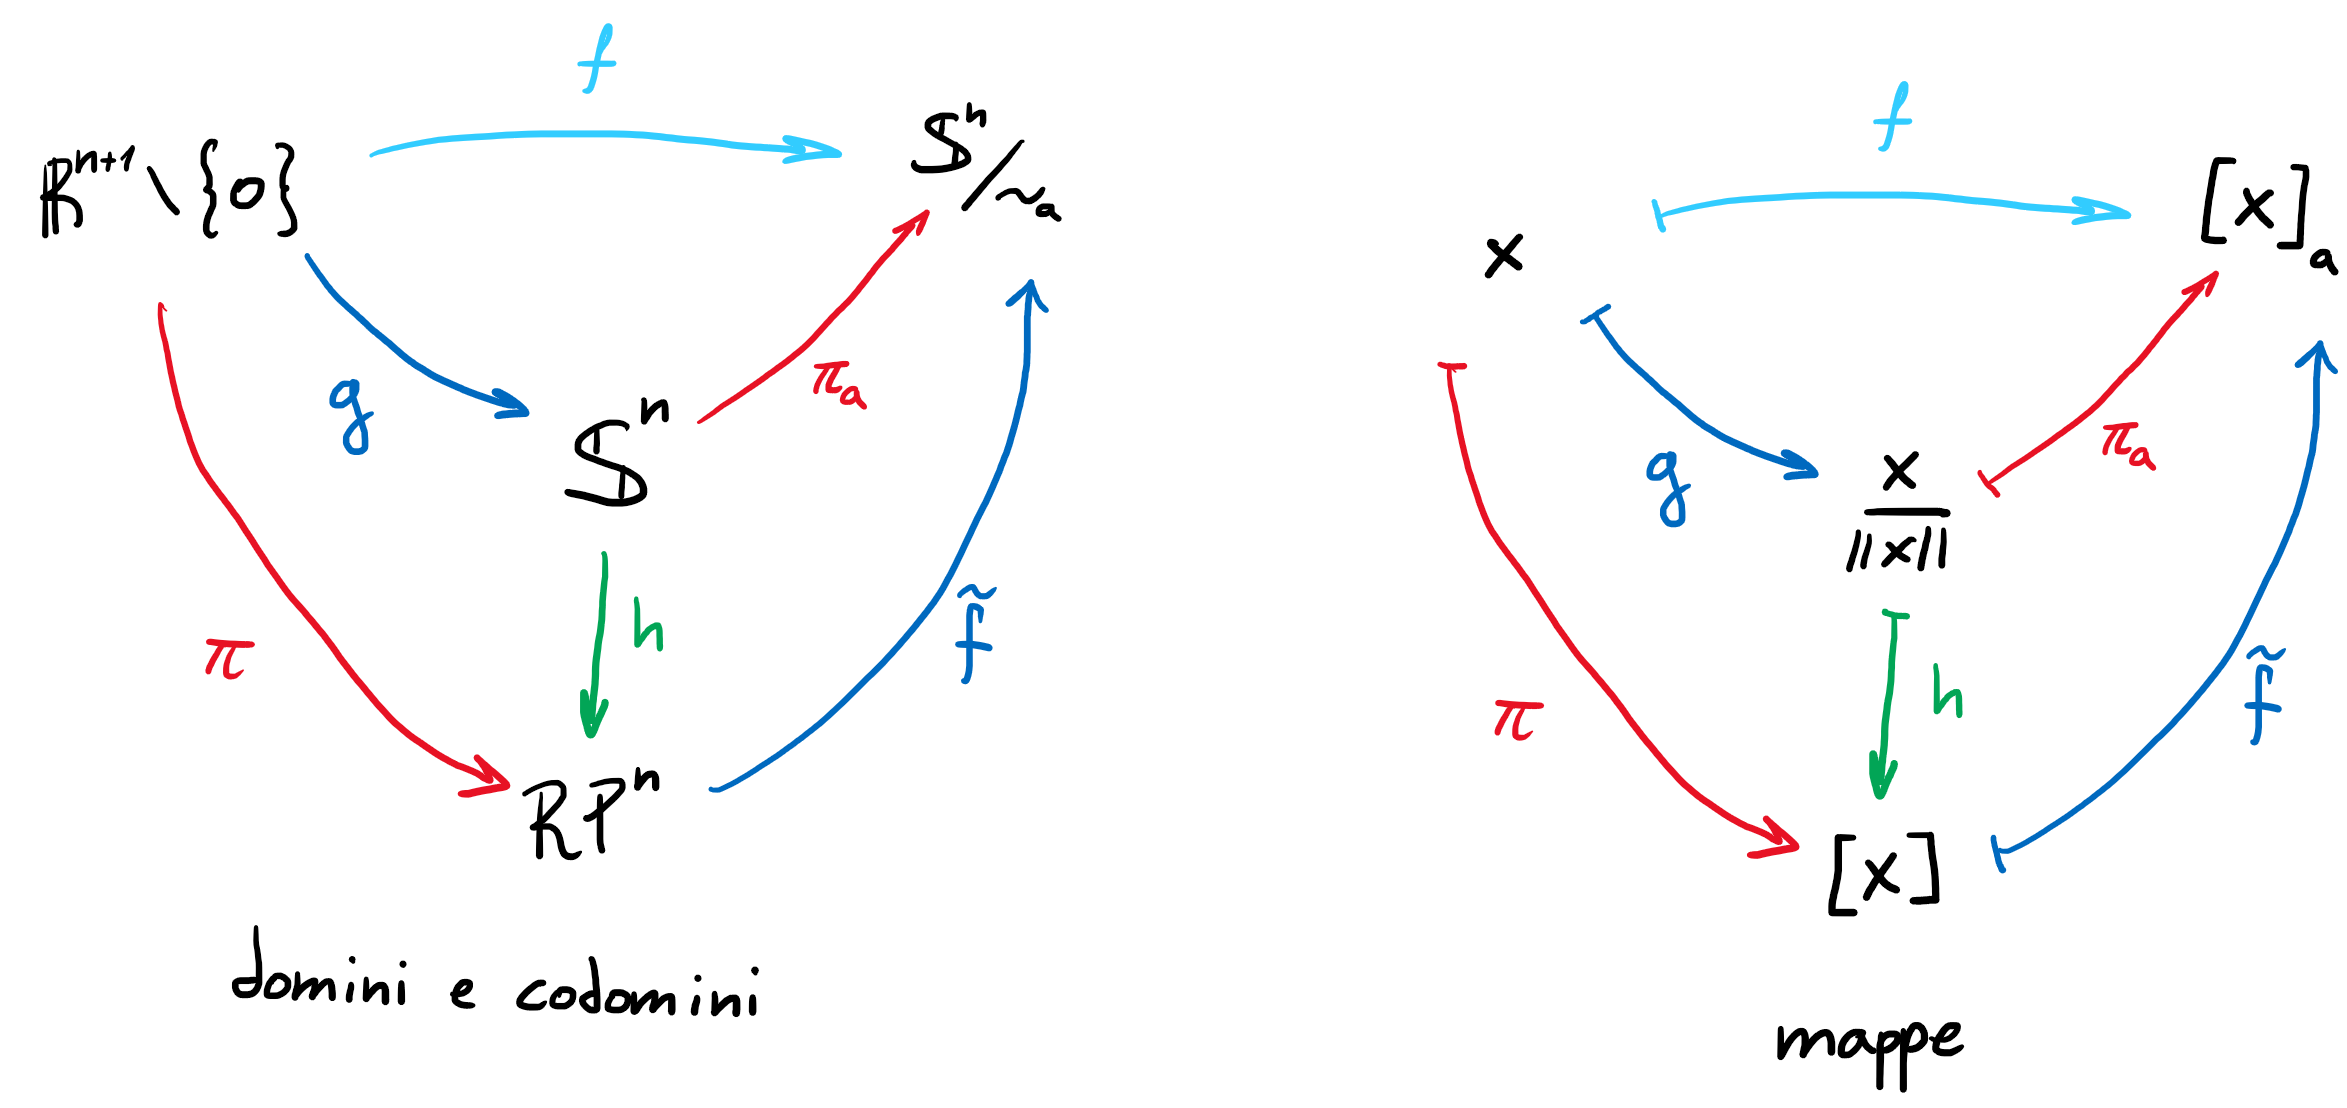
\includegraphics[width=0.7\textwidth,keepaspectratio]{img14}
	\end{figure}

	L'applicazione
	
	\begin{align}
		\begin{split}
			g : \R^{n+1} \setminus \{0\} &\to \S^{n}\\
			x &\mapsto \dfrac{x}{\norm{x}}
		\end{split}
	\end{align}

	prendendo un qualunque rappresentante di $ \R^{n+1} \setminus \{0\} $, potrebbe risultare in $ \pm x $, perciò usiamo l'applicazione
	
	\begin{align}
		\begin{split}
			f : \R^{n+1} \setminus \{0\} &\to \sfrac{\S^{n}}{\sim_{a}}\\
			x &\mapsto [x]_{a}
		\end{split}
	\end{align}

	la quale considera la classe dei punti antipodali nella sfera $ \S^{n} $. L'applicazione $ \tilde{f} $ che va dal proiettivo reale al quoziente è dunque ben definita tramite
	
	\begin{equation}
		\tilde{f}([x]) = [g(x)]_{a}
	\end{equation}

	Per asserire che $ \tilde{f} $ sia continua, possiamo dimostrare che $ f $ lo sia: quest'ultima applicazione è composizione di $ f = \pi_{a} \circ g $ dunque continua, perché le componenti di $ g $ sono continue e la proiezione sul quoziente è continua.\\
	L'ultimo passo è mostrare che $ \tilde{f} $ sia una bigezione\footnote{%
		Non possiamo utilizzare il lemma dell'applicazione chiusa perché altrimenti dovremmo utilizzare come assunzione che $ \mathcal{RP}^{n} $ sia compatto, ma questo è la tesi della dimostrazione.%
	}: per fare ciò prendiamo la sua inversa

	\begin{align}
		\begin{split}
			\tilde{f}^{-1} : \sfrac{\S^{n}}{\sim_{a}} &\to \mathcal{RP}^{n}\\
			[x]_{a} &\mapsto [x]
		\end{split}
	\end{align}

	la quale è continua perché composizione di applicazioni continue
	
	\begin{equation}
		\tilde{f}^{-1} = (\pi_{a} \circ g \circ \pi^{-1})^{-1} = \pi \circ g^{-1} \circ \pi_{a}^{-1}
	\end{equation}

	Analogamente, possiamo dire che sia continua perché due punti antipodali appartengono per forza alla stessa retta, i.e. $ p,q \in [x]_{a} \iff p,q \in [x] $.\\
	Avendo dimostrato che $ \tilde{f} $ è una bigezione continua, otteniamo che $ \mathcal{RP}^{n} \simeq \sfrac{\S^{n}}{\sim_{a}} $.
\end{proof}

\begin{corollary}
	$ \mathcal{RP}^{n} $ è compatto e connesso, in quanto lo è la sfera\footnote{%
		La sfera $ \S^{n} $ è connessa perché la sfera è densa nella sfera meno un punto (tramite proiezione stereografica in $ \R^{n} $) e la chiusura di uno spazio connesso è ancora connessa; per quanto riguarda la compattezza, il \textit{teorema di Heine-Borel} afferma che un sottoinsieme di $ \R^{n} $ è compatto se e solo se è chiuso e limitato.%
	} $ \S^{n} $ e la topologia quoziente preserva queste proprietà.
\end{corollary}

\subsubsection{\textit{Esempi}}

\paragraph{1.}

Se prendiamo $ n=1 $, $ \mathcal{RP}^{1} \simeq \S^{1} $: si può identificare $ \S^{1} $ con l'intervallo $ I $ omeomorfo alla semicirconferenza quozientato i due punti estremi di quest'ultima $ \{A,B\} $, i.e. $ \S^{1} \simeq \sfrac{I}{\{A,B\}} $, in modo tale che si prenda solo uno dei due punti antipodali.

\paragraph{2.}

Se prendiamo $ n=2 $, $ \mathcal{RP}^{2} \simeq \sfrac{\S^{2}}{\sim_{a}} $. Per visualizzarlo, prendiamo la calotta superiore di $ \S^{2} $ la quale è omeomorfa al disco unitario $ D_{1} $. Il disco unitario, pieno della proiezione della semicalotta in cui sono identificati i punti antipodali della circonferenza, rappresenta dunque il proiettivo reale $ \mathcal{RP}^{2} $.\\
Dimensioni più alte non sono rappresentabili tramite esempi nello spazio tridimensionale.

\subsubsection{Proprietà di $ \mathcal{RP}^{n} $}

Per dimostrare che $ \mathcal{RP}^{n} $ sia una varietà differenziabile dobbiamo prima dimostrare che sia una varietà topologica, dunque $ N_{2}+T_{2} $ con un atlante topologico, e poi far vedere che i cambi di carta siano lisci.\\
La dimostrazione che il proiettivo reale sia $ N_{2} $ passa per la proiezione

\begin{equation}
	\pi : \R^{n+1} \setminus \{0\} \to \dfrac{\R^{n+1} \setminus \{0\}}{\sim} = \mathcal{RP}^{n}
\end{equation}

in quanto questa applicazione preserva la proprietà di numerabilità $ N_{2} $: se lo spazio di partenza $ \R^{n+1} \setminus \{0\} $ è $ N_{2} $ (lo è perché sottoinsieme di $ \R^{n+1} $ il quale è a sua volta $ N_{2} $) allora, se l'applicazione $ \pi $ è aperta (equivalentemente, se $ \sim $ è aperta), lo è anche il proiettivo reale.\\
Perché $ \pi $ sia aperta, questa deve mandare aperti in aperti: sia l'aperto $ V \subset \R^{n+1} \setminus \{0\} $ e consideriamo $ \pi(V) $. Nella topologia quoziente, l'immagine $ \pi(V) $ è aperta se la sua controimmagine $ \pi^{-1}(\pi(V)) $ è aperta: $ \pi(x) $ con $ x \in V $ è l'identificazione di tutti i punti che appartengono alla stessa retta di $ x $; prendendo $ \pi^{-1}(\pi(x)) $ otteniamo non solo il punto $ x $ ma tutti i punti che appartengono alla retta identificata da $ x $ stesso, dunque considerando tutti i punti dell'aperto $ V $ otteniamo

\begin{equation}
	\pi^{-1}(\pi(V)) = \bigcup_{\lambda \in \R \setminus \{0\}} \{\lambda V\}
\end{equation}

che corrisponde al cono di rette passanti per l'origine individuato dai punti dell'aperto $ V $

\begin{figure}[H]
	\centering
	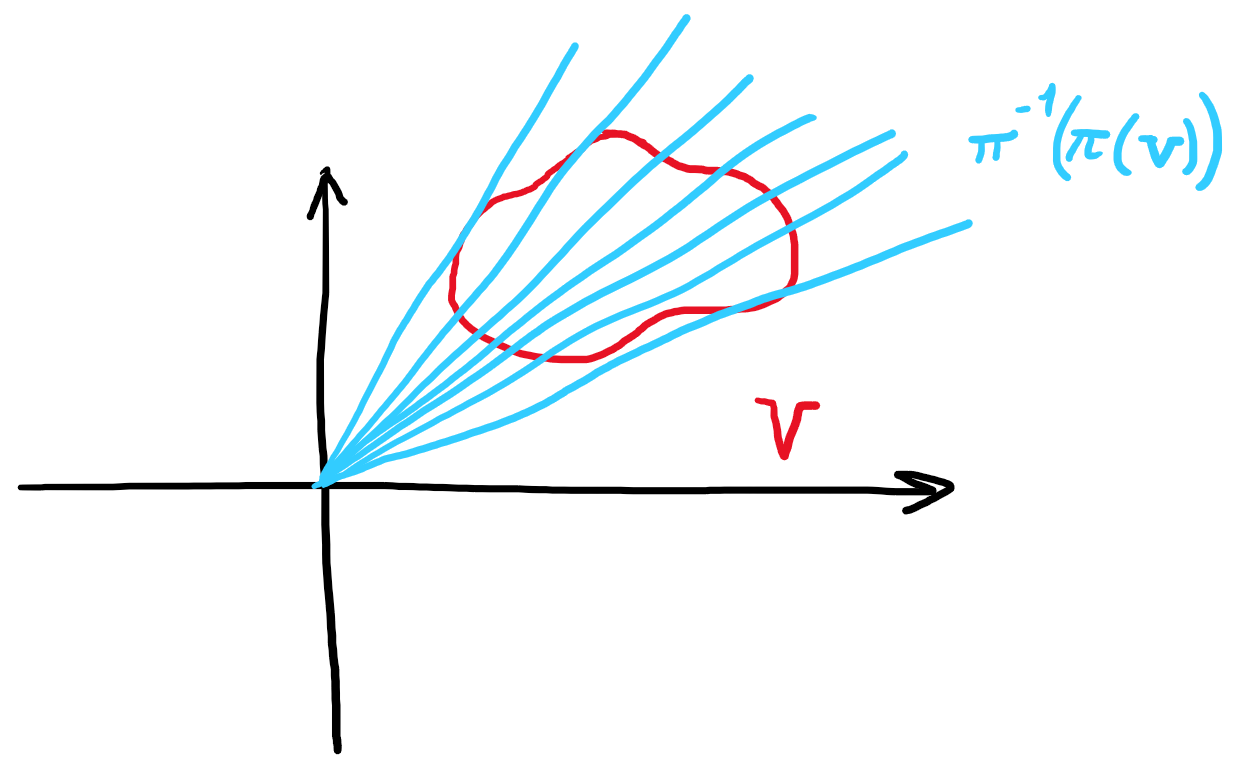
\includegraphics[width=0.45\textwidth,keepaspectratio]{img15}
\end{figure}

Fissando $ \lambda $, l'insieme

\begin{equation}
	\lambda V = \left\{ \lambda x \, \middle| \, x \in V \right\}
\end{equation}

è aperto perché omeomorfo a $ V $ tramite l'applicazione

\begin{align}
	\begin{split}
		\phi_{\lambda} : V &\to \lambda V\\
		x &\mapsto \lambda x
	\end{split}
\end{align}

la quale è continua con inversa continua

\begin{align}
	\begin{split}
		\phi_{\lambda}^{-1} : \lambda V &\to V\\
		\lambda^{-1} x &\mapsto x
	\end{split}
\end{align}

Essendo $ \lambda V $ aperto in $ \R \setminus \{0\} $, $ \pi^{-1}(\pi(V)) $ è aperto e dunque la proiezione $ \pi $ è aperta.\\
Se lo spazio di partenza $ \R \setminus \{0\} $ è $ N_{2} $ e la relazione di equivalenza $ \sim $ è aperta, allora lo spazio quoziente $ \mathcal{RP}^{n} $ è $ N_{2} $.\\\\
%
Sapendo che la proiezione $ \pi $ è aperta, possiamo usare il fatto che l'insieme

\begin{equation}
	R = \left\{ (x,y) \in \R^{n+1} \setminus \{0\} \times \R^{n+1} \setminus \{0\} \, \middle| \, y=\lambda x, \, \lambda \in \R \setminus \{0\} \right\} \subset \R^{n+1} \setminus \{0\} \times \R^{n+1} \setminus \{0\}
\end{equation}

sia chiuso per dimostrare che il proiettivo reale sia anche $ T_{2} $.\\
Per dimostrare che sia chiuso, consideriamo l'applicazione

\map{\phi}%
	{\R^{n+1} \setminus \{0\} \times \R^{n+1} \setminus \{0\}}{M_{n+1,2}(\R) = \R^{2(n+1)}}%
	{(x,y)}{\mqty[x & y]}

cioè che associa alle coppie di vettori $ (x,y) $ le matrici con $ (n+1) $ righe e $ 2 $ colonne costituite dai vettori $ x $ e $ y $ posti in colonne affiancate, i.e.

\begin{equation}
	x = \begin{bmatrix} x^{1} \\ \vdots \\ x^{n+1} \end{bmatrix}, \, y = \begin{bmatrix} y^{1} \\ \vdots \\ y^{n+1} \end{bmatrix} \quad \longmapsto \quad \begin{bmatrix} x & y \end{bmatrix} = \begin{bmatrix} x^{1} & y^{1} \\ \vdots & \vdots \\ x^{n+1} & y^{n+1} \end{bmatrix}
\end{equation}

L'applicazione $ \phi $ è un omeomorfismo perché la topologia prodotto di spazi euclidei coincide con la topologia euclidea, i.e. $ \R^{n} \times \R^{m} \simeq \R^{n+m} $ cioè sono topologicamente equivalenti (ogni aperto di uno è aperto dell'altro).\\
A questo punto, possiamo studiare la chiusura dell'immagine di $ R $ tramite $ \phi $

\begin{equation}
	\phi(R) = \left\{ \mqty[x & y] \in M_{n+1,2}(\R) \, \middle| \, \rank \left( \mqty[x & y] \right) = 1 \right\}
\end{equation}

La condizione per cui il rango delle matrici di questo insieme sia unitario è dovuta al fatto che queste matrici hanno le due colonne proporzionali tra loro, in quanto $ y= \lambda x $.

\begin{lemma}\label{lemma-clos-matrix}
	Sia l'insieme
	
	\begin{equation}
		X_{r}(n,m) = \left\{ A \in M_{n,m}(\R) \, \middle| \, \rank(A) \leqslant r \, \wedge \, r \leqslant \min\{n,m\} \right\}
	\end{equation}

	questo è chiuso in $ M_{n,m}(\R) = \R^{n m} $.
\end{lemma}

\begin{proof}
	Consideriamo l'applicazione
	
	\begin{align}
		\begin{split}
			f :  M_{n,m}(\R) &\to \R^{d}\\
			A &\mapsto (m_{11},\dots,m_{nm})
		\end{split}
	\end{align}

	che mappa le matrici $ A \in M_{n,m}(\R) $ in $ d $-uple\footnote{%
		Il numero totale di minori di ordine $ r $ per una matrice $ A \in M_{n,m}(\R) $ è $ d = \begin{pmatrix} m \\ r+1 \end{pmatrix} \begin{pmatrix} n \\ r+1 \end{pmatrix} $.%
	} di minori $ m_{ij} = \det(A_{ij}) $ di $ A $ di ordine $ r < \min\{n,m\} $, dove le $ A_{ij} $ sono le sottomatrici ricavate da $ A $ rimuovendo la $ i $-esima riga e la $ j $-esima colonna. Questa applicazione è continua perché è composizione dell'applicazione che rimuove righe e colonne alla matrice $ A $ e il determinante di questa stessa matrice (entrambe le applicazioni sono continue).\\
	Una matrice $ A $ ha rango $ \rank(A) \leqslant r $ se e solo se tutti i minori di ordine $ r+1 $ sono nulli, dunque l'insieme $ X_{r}(n,m) $ è la controimmagine di $ 0 \in \R^{d} $ tramite l'applicazione continua $ f $: essendo $ \{0\} $ chiuso in $ \R^{d} $ perché $ \R^{d} $ è di Hausdorff, allora anche la sua controimmagine tramite $ f $, i.e. $ f^{-1}(0) = X_{r}(n,m) $, è chiusa in $ M_{n,m}(\R) $.
\end{proof}

Seguendo questo ragionamento, possiamo pensare a $ \phi(R) $ come l'intersezione dell'immagine dello spazio di Hausdorff $ \R^{n+1} \setminus \{0\} \times \R^{n+1} \setminus \{0\} $ tramite $ \phi $ con $ X_{1}(n+1,2) $, il quale è un chiuso

\begin{equation}
	\phi(R) = X_{1}(n+1,2) \cap \phi(\R^{n+1} \setminus \{0\} \times \R^{n+1} \setminus \{0\})
\end{equation}

Essendo dunque $ \phi(R) $ intersezione di un chiuso con lo spazio d'interesse, questo rende $ \phi(R) $ chiuso in $ \phi(\R^{n+1} \setminus \{0\} \times \R^{n+1} \setminus \{0\}) $, dunque $ R $ è chiuso in $ \R^{n+1} \setminus \{0\} \times \R^{n+1} \setminus \{0\} $.\\
Questo prova che $ \mathcal{RP}^{n} $ sia $ T_{2} $.\\\\
%
A questo punto, costruiamo un atlante topologico per il proiettivo reale.\\
Siano gli $ n+1 $ insiemi

\begin{equation}
	U_{i} = \{ [(a^{0},\dots,a^{n})] = \pi(a^{0},\dots,a^{n}) \in \mathcal{RP}^{n} \mid a^{i} \neq 0 \} \qcomma i=0,\dots,n
\end{equation}

i cui elementi sono dunque le classi di $ n+1 $-uple di cui la componente $ i $-esima sia diversa da zero. Si può anche pensare a questi insieme come $ U_{i} = \pi(V_{i}) $ con

\begin{equation}
	V_{i} = \{ (a^{0},\dots,a^{n}) \in \R^{n+1} \setminus \{0\} \mid a^{i} \neq 0 \} \subset \R^{n+1} \setminus \{0\} \qcomma i=0,\dots,n
\end{equation}

Gli insiemi $ U_{i} $ sono aperti in $ \mathcal{RP}^{n} $ perché $ \pi $ è aperta e i $ V_{i} $ sono aperti in $ \R^{n+1} \setminus \{0\} $.\\
Questi insiemi sono un ricoprimento per $ \mathcal{RP}^{n} $

\begin{equation}
	\bigcup_{i=0}^{n} U_{i} = \mathcal{RP}^{n}
\end{equation}

o equivalentemente

\begin{equation}
	\bigcup_{i=0}^{n} V_{i} = \R^{n+1} \setminus \{0\}
\end{equation}

perché ogni punto di $ \R^{n+1} \setminus \{0\} $ avrà almeno una coordinata diversa da zero e, conseguentemente, la sua proiezione su $ \mathcal{RP}^{n} $ avrà anch'essa almeno una coordinata diversa da zero.\\
Siano le applicazioni

\begin{align}
	\begin{split}
		\phi_{i} : U_{i} &\to \R^{n}\\
		[(a^{0},\dots,a^{n})] &\mapsto \left( \dfrac{a^{0}}{a^{i}}, \dfrac{a^{1}}{a^{i}}, \dots, \dfrac{a^{i-1}}{a^{i}}, \dfrac{a^{i+1}}{a^{i}}, \dots, \dfrac{a^{n}}{a^{i}} \right)
	\end{split}
\end{align}

con $ i=0,\dots,n $, cioè cancelliamo l'$ i $-esima componente dal vettore nell'immagine e dividiamo tutte le altre per $ a^{i} $.\\
Queste applicazioni sono ben definite in quanto la proporzionalità tra gli elementi della classe di equivalenza $ [(a^{0},\dots,a^{n})] $ viene assorbita nei rapporti in immagine.\\
Essendo l'unione degli insiemi $ U_{i} $ un ricoprimento per $ \mathcal{RP}^{n} $, dimostrando che le $ \phi_{i} $ sono degli omeomorfismi, facciamo vedere che $ \mathfrak{M} = \{(U_{i},\phi_{i})\} $ è un atlante topologico per $ \mathcal{RP}^{n} $.\\
Queste applicazioni fanno parte del diagramma

\begin{figure}[H]
	\centering
	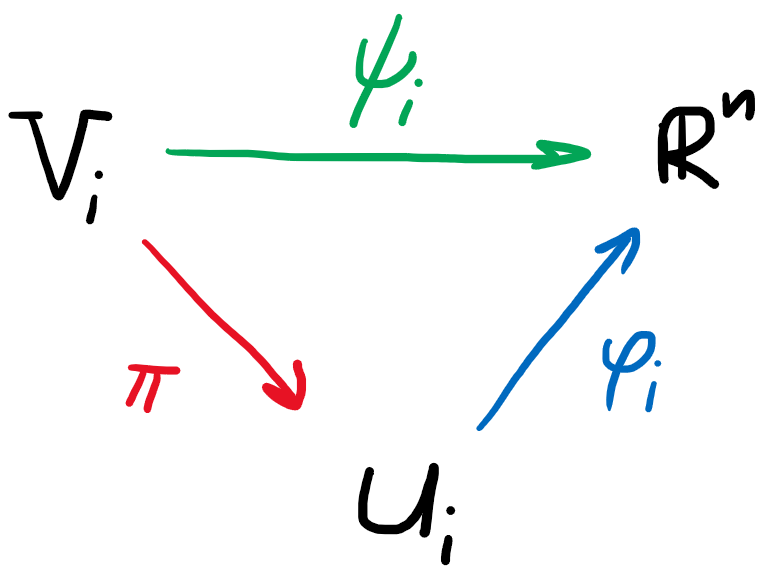
\includegraphics[width=0.3\textwidth,keepaspectratio]{img16}
\end{figure}

dove

\begin{align}
	\begin{split}
		\psi_{i} : V_{i} &\to \R^{n}\\
		(a^{0},\dots,a^{n}) &\mapsto \left( \dfrac{a^{0}}{a^{i}}, \dfrac{a^{1}}{a^{i}}, \dots, \dfrac{a^{i-1}}{a^{i}}, \dfrac{a^{i+1}}{a^{i}}, \dots, \dfrac{a^{n}}{a^{i}}, \right)
	\end{split}
\end{align}

la quale è continua perché tutte le sue componenti sono continue. A questo punto, le $ \phi_{i} $ rendono commutativo questo diagramma (le $ \psi_{i} $ sono costanti sulle classi di equivalenza) perciò le $ \phi_{i} $ sono continue.\\
Le applicazioni inverse sono

\begin{align}
	\begin{split}
		\phi_{i}^{-1} : \R^{n} &\to U_{i}\\
		(x^{1},\dots,x^{n}) &\mapsto [(x^{1},\dots,x^{i-1},1,x^{i},x^{i+1},\dots,x^{n})]
	\end{split}
\end{align}

siccome è presente la componente $ i $-esima uguale ad 1, la classe $ [(x^{1},\dots,x^{i-1},1,x^{i},x^{i+1},\dots,x^{n})] $ appartiene a $ \mathcal{RP}^{n} $ anche se $ (x^{1},\dots,x^{n}) = (0,\dots,0) $. Queste applicazioni sono le inverse di $ \phi_{i} $ perché

\begin{align}
	\begin{split}
		(\phi_{i} \circ \phi_{i}^{-1})(x^{1},\dots,x^{n}) &= \phi_{i}([(x^{1},\dots,x^{i-1},1,x^{i},x^{i+1},\dots,x^{n})])\\
		&= (x^{1},\dots,x^{n})\\\\
		%
		(\phi^{-1}_{i} \circ \phi_{i})([(a^{0},\dots,a^{n})]) &= \phi_{i}^{-1} \left( \dfrac{a^{0}}{a^{i}}, \dfrac{a^{1}}{a^{i}}, \dots, \dfrac{a^{i-1}}{a^{i}}, \dfrac{a^{i+1}}{a^{i}}, \dots, \dfrac{a^{n}}{a^{i}} \right)\\
		&= \left[ \left( \dfrac{a^{0}}{a^{i}}, \dfrac{a^{1}}{a^{i}}, \dots, \dfrac{a^{i-1}}{a^{i}}, 1, \dfrac{a^{i+1}}{a^{i}}, \dots, \dfrac{a^{n}}{a^{i}} \right) \right]\\
		&= [(a^{0},\dots,a^{i-1},a^{i},a^{i+1},\dots,a^{n})]\\
		&= [(a^{0},\dots,a^{n})]
	\end{split}
\end{align}

e sono continue. Dunque abbiamo dimostrato che le $ \phi_{i} $ sono omeomorfismi e quindi $ \mathfrak{M} = \{(U_{i},\phi_{i})\}_{i=0,\dots,n} $ è un atlante topologico per $ \mathcal{RP}^{n} $.\\
Dimostriamo ora che $ \mathfrak{M} $ è un atlante differenziabile di $ \mathcal{RP}^{n} $, cioè dobbiamo far vedere che le sue carte siano $ C^{\infty} $-compatibili tra loro: siano $ i,j=0,\dots,n $ con $ i<j $ e prendiamo i cambi di carta

\begin{align}
	\begin{split}
		\phi_{i} \circ \phi_{j}^{-1} : \phi_{j}(U_{i \cap U_{j}}) \to \phi_{i}(U_{i \cap U_{j}})\\
		\phi_{j} \circ \phi_{i}^{-1} : \phi_{i}(U_{i \cap U_{j}}) \to \phi_{j}(U_{i \cap U_{j}})
	\end{split}
\end{align}

dove un elemento in $ U_{i} \cap U_{j} $ ha sia la $ i $-esima che la $ j $-esima componente diversa da zero.\\
Dunque

\begin{align}
	\begin{split}
		(\phi_{i} \circ \phi_{j}^{-1})(x^{1},\dots,x^{n}) &= \phi_{i}([(x^{1},\dots,x^{j-1},1,x^{j},x^{j+1},\dots,x^{n})])\\
		&= \left( \dfrac{x^{1}}{x_{i}}, \dots, \dfrac{x^{i-1}}{x_{i}}, \dfrac{x^{i+1}}{x_{i}}, \dots, \dfrac{x^{j-1}}{x_{i}}, \dfrac{1}{x_{i}}, \dfrac{x^{j+1}}{x_{i}}, \dots, \dfrac{x^{n}}{x_{i}} \right)\\\\
		%
		(\phi_{j} \circ \phi_{i}^{-1})(x^{1},\dots,x^{n}) &= \phi_{j}([(x^{1},\dots,x^{i-1},1,x^{i},x^{i+1},\dots,x^{n})])\\
		&= \left( \dfrac{x^{1}}{x_{i}}, \dots, \dfrac{x^{i-1}}{x_{j}}, \dfrac{1}{x_{j}}, \dfrac{x^{i+1}}{x_{j}}, \dots, \dfrac{x^{j-1}}{x_{j}}, \dfrac{x^{i+j}}{x_{j}}, \dots, \dfrac{x^{n}}{x_{j}} \right)
	\end{split}
\end{align}

entrambi i cambi di carta sono lisci quindi $ \mathfrak{M} $ è un atlante differenziabile: questo dimostra l'esistenza di un atlante differenziabile massimale che rende $ \mathcal{RP}^{n} $ una varietà differenziabile.

\subsection{Grassmanniana come varietà differenziabile}

Siano $ k,n \in \N $ con $ k \leqslant n $, definisco la \textit{grassmanniana} $ G(k,n) $ come l'insieme di tutti i sottospazi vettoriali di $ \R^{n} $ di dimensione $ k $.\\
Essendo $ \mathcal{RP}^{n} $ l'insieme di tutti i sottospazi vettoriali di dimensione 1 (i.e. rette) di $ \R^{n+1} $, si ha che

\begin{equation}
	G(1,n) = \mathcal{RP}^{n-1}
\end{equation}

dunque la grassmanniana può essere pensata come la generalizzazione del proiettivo reale.\\
Vogliamo ora dotare la grassmanniana di una struttura di varietà differenziabile, in modo analogo al proiettivo reale.

\begin{remark}
	Un $ k $-spazio vettoriale\footnote{%
		Cioè uno spazio vettoriale di dimensione $ k $.%
	} $ S $ di $ \R^{n} $ è determinato da $ a_{1},\dots,a_{k} $ vettori linearmente indipendenti di $ \R^{n} $ quindi da una matrice $ A = \begin{bmatrix} a_{1} & \dots & a_{k} \end{bmatrix} \in M_{n,k}(\R^{n}) $ con rango $ \rank(A) = k $.
\end{remark}

Due matrici $ A $ e $ B $ rappresentano lo stesso $ k $-spazio vettoriale se e solo se le colonne di una sono linearmente dipendenti dalle colonne dell'altra, i.e. $ B = A g $ dove $ g \in GL_{k}(\R) $ ($ g $ è invertibile), perciò le matrici $ A $ e $ B $ sono legate da una trasformazione lineare (o cambio di base) nello spazio generato dai vettori colonna che compongono le matrici.\\
Consideriamo la relazione di equivalenza $ \sim $ sull'insieme

\begin{equation}
	F(k,n) = \left\{ A \in M_{n,k}(\R) \, \middle| \, \rank(A) = k \right\} \subset M_{n,k}(\R) = \R^{nk}
\end{equation}

definita come

\begin{equation}
	A \sim B \, \iff \, \E g \in GL_{k}(\R) \, \mid \, B = A g
\end{equation}

Possiamo dunque affermare che

\begin{equation}
	G(k,n) = \sfrac{F(k,n)}{\sim}
\end{equation}

Per ogni $ k $-spazio $ S $ esiste dunque una classe di equivalenza $ [A] $ di tutte le matrici legate tra loro da una trasformazione lineare le cui colonne generano lo spazio stesso. Tra la classe di equivalenza e lo spazio è presente una bigezione.\\
L'intento è di dimostrare che $ G(k,n) $ sia una varietà differenziabile di dimensione

\begin{equation}
	\dim (G(k,n)) = k (n-k)
\end{equation}

Come primo passo associamo la topologia quoziente a $ \sfrac{F(k,n)}{\sim} $: l'insieme $ F(k,n) $ è un aperto in quanto il suo complementare

\begin{equation}
	M_{n,k}(\R) \setminus F(k,n) = \left\{ A \in M_{n,k}(\R) \, \middle| \, \rank(A) \leqslant k \right\}
\end{equation}

è chiuso per il Lemma \ref{lemma-clos-matrix}.\\
Per dimostrare che lo spazio $ G(k,n) $ sia $ N_{2} $, usiamo la Proposizione \ref{prop-n2}: $ F(k,n) $ è $ N_{2} $ in quanto sottospazio di $ M_{n,k}(\R) $ e la proiezione $ \pi : F(k,n) \to \sfrac{F(k,n)}{\sim} = G(k,n) $ è aperta (equivalentemente $ \sim $ è aperta).
La dimostrazione che $ \pi $ sia aperta è analoga a quella per il proiettivo: preso un aperto, la sua immagine deve essere aperta, il quale si dimostra facendo vedere che la controimmagine di quest'ultima sia aperta.\\
Sia $ V $ un aperto di $ F(k,n) $, possiamo scrivere

\begin{align}
	\begin{split}
		\pi^{-1}(\pi(V)) = \bigcup_{g \in GL_{k}(\R)} V g
	\end{split}
\end{align}

dove

\begin{equation}
	V g = \{ A g \in M_{n,k}(\R) \mid A \in V \wedge g \in GL_{k}(\R) \}
\end{equation}

Prendiamo l'applicazione

\map{\phi_{g}}%
	{F(k,n)}{F(k,n)}%
	{A}{A g}

questo è un omeomorfismo dunque $ \phi_{g}(V) = V g $ è un aperto perché $ V $ è aperto. Questo dimostra che $ \pi^{-1}(\pi(V)) $ sia aperto in quanto unione di aperti e quindi $ G(k,n) $ è $ N_{2} $.\\\\
%
Per dimostrare che lo spazio $ G(k,n) $ sia $ T_{2} $, usiamo la Proposizione \ref{prop-t2}: prendiamo l'insieme

\begin{equation}
	R = \{ (A,B) \in F(k,n) \times F(k,n) \mid B = A g, \, g \in GL_{k}(\R) \}
\end{equation}

per dimostrare che sia chiuso, consideriamo l'applicazione

\map{\phi}%
	{M_{n,k}(\R) \times M_{n,k}(\R)}{M_{n,2k}(\R)}%
	{(A,B)}{\mqty(A & B)}

cioè $ \phi $ "affianca" due matrici rendendole un'unica matrice con il doppio delle colonne.

\begin{figure}[H]
	\centering
	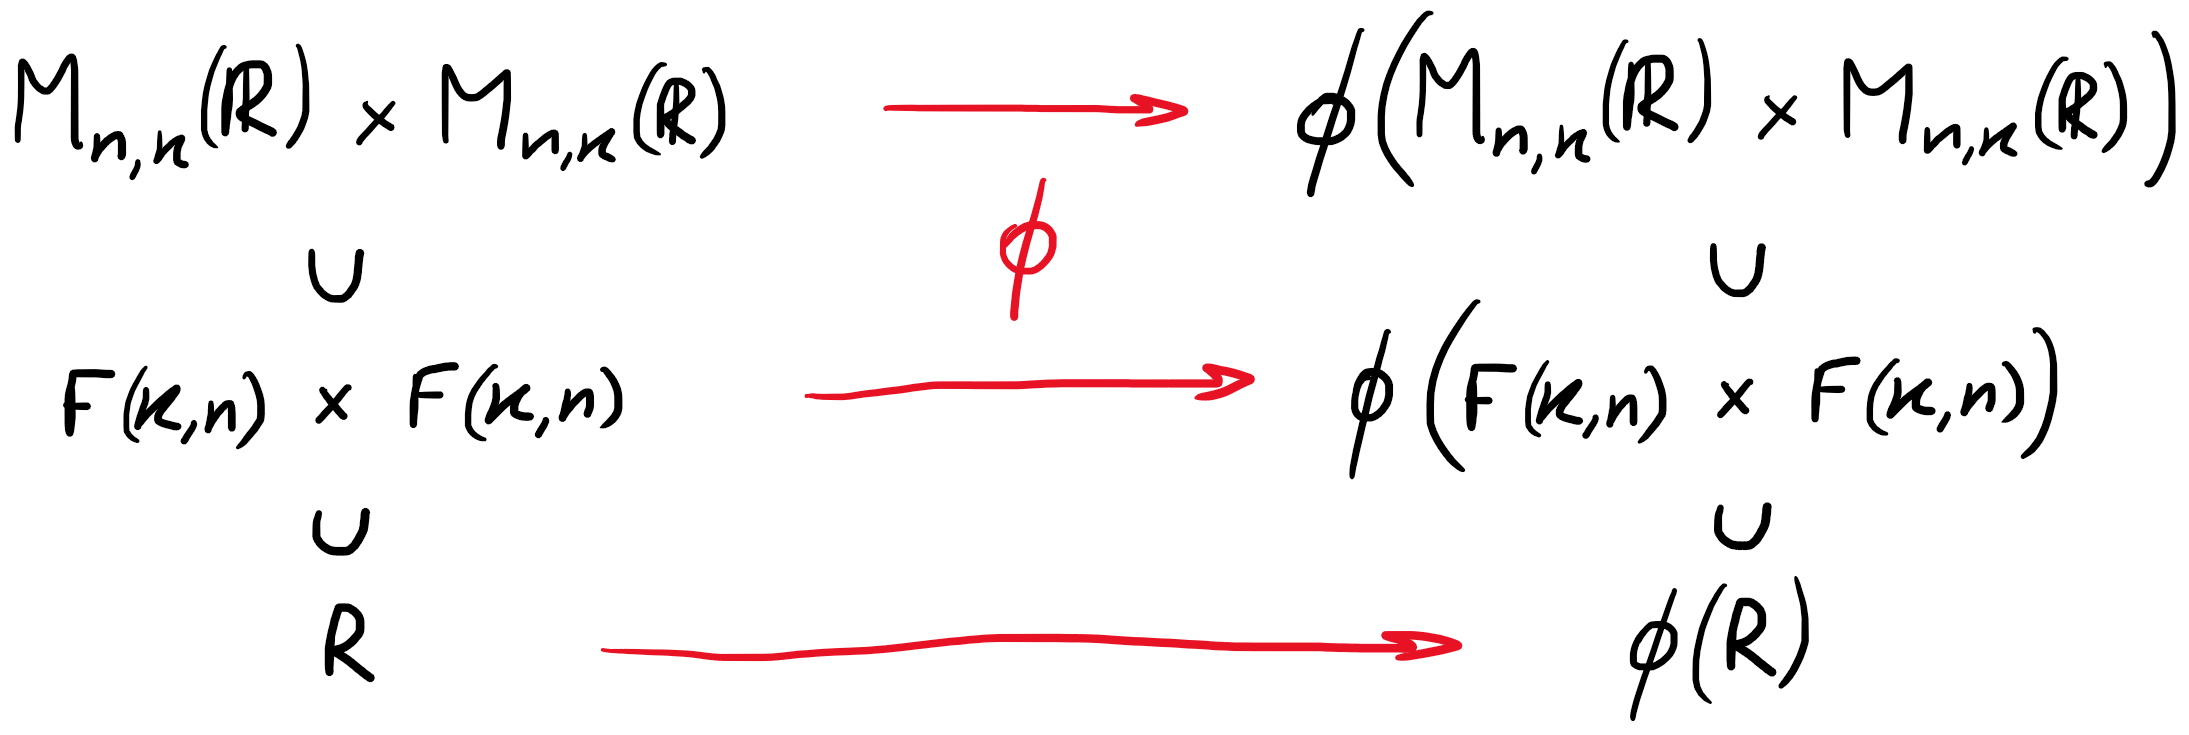
\includegraphics[width=0.6\textwidth,keepaspectratio]{img17}
\end{figure}

Essendo $ \phi $ un omeomorfismo, per dimostrare che $ R $ sia chiuso in $ F(k,n) \times F(k,n) $, basta dimostrare che $ \phi(R) $ sia chiuso in $ \phi(F(k,n) \times F(k,n)) $.\\
Dal Lemma \ref{lemma-clos-matrix} prendiamo la definizione del seguente insieme

\begin{equation}
	X_{r}(n,m) = \left\{ A \in M_{n,m}(\R) \, \middle| \, \rank(A) \leqslant r \, \wedge \, r \leqslant \min\{n,m\} \right\}
\end{equation}

dunque l'immagine di $ R $ è pari a

\begin{equation}
	\phi(R) = \{ A \in M_{n,2k}(\R) \mid \rank(A) \leqslant k \} = \phi(F(k,n) \times F(k,n)) \cap X_{k}(n,2k)
\end{equation}

in quanto $ \phi(R) $ è l'insieme delle matrici $ n \times 2k $ le quali hanno rango al massimo uguale a $ k $ (in quanto formate da due matrici di rango $ k $ legate tra loro da $ g $). Essendo $ X_{k}(n,2k) $ chiuso, allora anche $ \phi(R) $ è chiuso in $ \phi(F(k,n) \times F(k,n)) $ e dunque $ R $ è chiuso in $ F(k,n) \times F(k,n) $, dimostrando che $ G(k,n) $ è $ T_{2} $.\\
Vedi Esercizio \ref{es2-5}. \textbf{l 9 m 28.20}

\subsubsection{Calcolo esplicito per $ G(2,4) $}

Mostriamo ora che $ G(k,n) $ sia una varietà differenziabile per $ k=2 $ e $ n=4 $ (il ragionamento è analogo per altri valori di $ k $ e $ n $); la dimensione è $ \dim(G(2,4)) = 2(4-2) = 4 $.\\
Consideriamo gli aperti di $ G(2,4) $

\begin{equation}
	U_{ij} = \left\{ [A] \in G(2,4) \, \middle| \, A_{ij} \in GL_{2}(\R) \right\}
\end{equation}

i.e. $ A_{ij} $ è invertibile, dove $ A_{ij} $ è la matrice quadrata $ 2 \times 2 $ che si ottiene considerando le righe $ i $ e $ j $ di $ A $, i.e.

\begin{equation}
	[A] = \left[ \mqty( a_{11} & a_{12} \\ a_{21} & a_{22} \\ a_{31} & a_{32} \\ a_{41} & a_{42} ) \right] \quad \longrightarrow \quad%
	\begin{cases}
		A_{12} = \mqty( a_{11} & a_{12} \\ a_{21} & a_{22} ) & A_{23} = \mqty( a_{21} & a_{22} \\ a_{31} & a_{32} )\\\\
		%
		A_{13} = \mqty( a_{11} & a_{12} \\ a_{31} & a_{32} ) & A_{24} = \mqty( a_{21} & a_{22} \\ a_{41} & a_{42} )\\\\
		%
		A_{14} = \mqty( a_{11} & a_{12} \\ a_{41} & a_{42} ) & A_{34} = \mqty( a_{31} & a_{32} \\ a_{41} & a_{42} )
	\end{cases}
\end{equation}

Preso $ B = A g $ (i.e. $ A \sim B $), abbiamo che $ A_{ij} $ è invertibile se e solo se $ B_{ij} $ è invertibile

\begin{align}
	\begin{split}
		A g &= B\\
		\mqty( a_{11} & a_{12} \\ a_{21} & a_{22} \\ a_{31} & a_{32} \\ a_{41} & a_{42} ) \mqty( g_{11} & g_{12} \\ g_{21} & g_{22} ) &= \mqty( b_{11} & b_{12} \\ b_{21} & b_{22} \\ b_{31} & b_{32} \\ b_{41} & b_{42} )\\
		\mqty( a_{11} g_{11} + a_{12} g_{21} & a_{11} g_{12} + a_{12} g_{22} \\ a_{21} g_{11} + a_{22} g_{21} & a_{21} g_{12} + a_{22} g_{22} \\ a_{31} g_{11} + a_{32} g_{21} & a_{31} g_{12} + a_{32} g_{22} \\ a_{41} g_{11} + a_{42} g_{21} & a_{41} g_{12} + a_{42} g_{22} ) &= \mqty( b_{11} & b_{12} \\ b_{21} & b_{22} \\ b_{31} & b_{32} \\ b_{41} & b_{42} )
	\end{split}
\end{align}

perciò $ A_{ij} g = B_{ij} $ e dunque la scelta del rappresentante di $ [A] $ è irrilevante.\\
Gli insiemi $ U_{ij} $ sono aperti in quanto immagini di aperti $ V_{ij} $ tramite la proiezione $ U_{ij} = \pi(V_{ij}) $, dove

\begin{equation}
	V_{ij} = \left\{ A \in F(2,4) \, \middle| \, A_{ij} \in GL_{2}(\R) \right\}
\end{equation}

è aperto in $ F(2,4) $ perché complementare di un chiuso.\\
Inoltre abbiamo che l'unione degli $ U_{ij} $ è un ricoprimento di $ G(2,4) $

\begin{equation}
	G(2,4) = \bigcup_{i,j=1}^{4} U_{ij}
\end{equation}

in quanto l'unione degli $ V_{ij} $ è un ricoprimento di $ F(2,4) $

\begin{equation}
	F(2,4) = \bigcup_{i,j=1}^{4} V_{ij}
\end{equation}

perché una matrice, per essere di rango $ k=2 $ e quindi appartenere a $ F(2,4) $, deve avere i suoi minori $ m_{ij} = \det(V_{ij}) $ di ordine 2 diversi da zero.\\
Per costruire le carte dell'atlante, consideriamo l'applicazione

\begin{align}
	\begin{split}
		\phi_{12} : U_{12} &\to M_{2}(\R) = \R^{4}\\
		[A] &\mapsto A_{34} (A_{12})^{-1}
	\end{split}
\end{align}

la quale è ben definita in quanto, se considerassimo un rappresentante diverso $ B = A g $, avremmo che $ B_{34} = A_{34} g $ e $ B_{12} = A_{12} g $, dunque

\begin{align}
	\begin{split}
		A_{34} (A_{12})^{-1} &= B_{34} \, g \, (B_{12} \, g)^{-1}\\
		&= B_{34} \, g \, g^{-1} \, (B_{12})^{-1}\\
		&= B_{34} (B_{12})^{-1}
	\end{split}
\end{align}

Le altre applicazioni sono analoghe, dunque

\begin{align}
	\begin{split}
		\phi_{ij} : U_{ij} &\to M_{2}(\R) = \R^{4}\\
		[A] &\mapsto A_{lm} (A_{ij})^{-1}
	\end{split}
\end{align}

dove $ \{i,j,l,m\}=\{1,2,3,4\} $.\\
Verifichiamo che le $ \phi_{ij} $ siano omeomorfismi, prendendo come esempio $ \phi_{12} $, dimostrando che sia continua e con inversa continua. La continuità è data dal seguente diagramma

\begin{figure}[H]
	\centering
	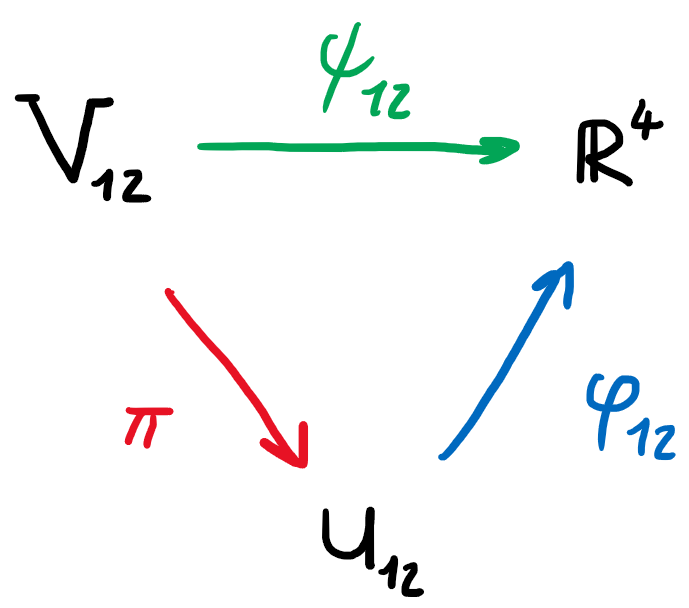
\includegraphics[width=0.3\textwidth,keepaspectratio]{img18}
\end{figure}

dove $ \psi_{12}(A) = A_{34} (A_{12})^{-1} $ è continua e costante sulle classe di equivalenza.\\
La sua inversa è

\map{(\phi_{12})^{-1}}%
	{M_{2}(\R) = \R^{4}}{U_{12}}%
	{\mqty( c_{11} & c_{12} \\ c_{21} & c_{22} )}{\left[ \mqty( 1 & 0 \\ 0 & 1 \\ c_{11} & c_{12} \\ c_{21} & c_{22} ) \right]}

perché

\begin{equation}
	\phi_{12} \circ (\phi_{12})^{-1} = \id_{\R^{4}}
\end{equation}

e dall'altro lato

\begin{align}
	\begin{split}
		((\phi_{12})^{-1} \circ \phi_{12})([A]) &= (\phi_{12})^{-1}(A_{34} (A_{12})^{-1})\\
		&= \left[ \mqty( \id_{2 \times 2} \\ A_{34} (A_{12})^{-1} ) \right]\\
		&= \left[ \mqty( A_{12} \\ A_{34} ) \right]\\
		&= [A]
	\end{split}
\end{align}

dunque anche

\begin{equation}
	(\phi_{12})^{-1} \circ \phi_{12} = \id_{U_{12}}
\end{equation}

L'inversa è continua perché composizione di due funzioni continue

\begin{equation}
	(\phi_{12})^{-1} = (\psi_{12} \circ \pi^{-1})^{-1} = \pi \circ (\psi_{12})^{-1}
\end{equation}

dove

\map{(\psi_{12})^{-1}}%
	{\R^{4}}{\R^{8}}%
	{\mqty( c_{11} & c_{12} \\ c_{21} & c_{22} )}{\mqty( 1 & 0 \\ 0 & 1 \\ c_{11} & c_{12} \\ c_{21} & c_{22} )}

Questo mostra l'esistenza di un atlante topologico $ \mathfrak{M} = \{(U_{ij},\phi_{ij})\}_{i,j=1,\dots,4} $ per $ G(2,4) $: affinché questo atlante sia differenziabile, mostriamo che i cambi di carte (e.g. $ \phi_{12} $ e $ \phi_{13} $)

\begin{align}
	\begin{split}
		\phi_{12} \circ (\phi_{13})^{-1} : \phi_{13} (U_{12} \cap U_{13}) \to \phi_{12} (U_{12} \cap U_{13})\\
		\phi_{13} \circ (\phi_{12})^{-1} : \phi_{12} (U_{12} \cap U_{13}) \to \phi_{13} (U_{12} \cap U_{13})
	\end{split}
\end{align}

siano lisci

\begin{align}
	\begin{split}
		(\phi_{13} \circ (\phi_{12})^{-1}) (C) &= \left( \mqty( c_{11} & c_{12} \\ c_{21} & c_{22} ) \right)\\\\
		&= \phi_{13} \left( \left[ \mqty( 1 & 0 \\ 0 & 1 \\ c_{11} & c_{12} \\ c_{21} & c_{22} ) \right] \right)\\\\
		&= \mqty( 0 & 1 \\ c_{21} & c_{22} ) \mqty( 1 & 0 \\ c_{11} & c_{12} )^{-1}\\\\
		&= \mqty( 0 & 1 \\ c_{21} & c_{22} ) \dfrac{1}{c_{12}} \mqty( c_{12} & 0 \\ -c_{11} & 1 )\\\\
		&= \dfrac{1}{c_{12}} \mqty( -c_{11} & 1 \\ c_{12} c_{21} - c_{11} c_{22} & c_{22} )\\\\
		&= \dfrac{1}{c_{12}} \mqty( -c_{11} & 1 \\ -\det(C) & c_{22} )
	\end{split}
\end{align}

dove $ c_{12} \neq 0 $ in quanto $ \det(C_{13}) = c_{12} $ e questa deve essere invertibile, abbiamo dunque

\map{\phi_{13} \circ (\phi_{12})^{-1}}%
	{\R^{4}}{\R^{4}}%
	{C = (c_{11}, c_{12}, c_{21}, c_{22})}{\dfrac{1}{c_{12}} (-c_{11}, 1, -\det(C), c_{22})}

la quale ha ogni componente liscia, proprio perché $ c_{12} \neq 0 $. Il ragionamento è analogo per gli altri cambi di carte: questo dimostra che $ \mathfrak{M} = \{(U_{ij},\phi_{ij})\}_{i,j=1,\dots,4} $ è un atlante differenziabile per $ G(2,4) $ e dunque esiste un atlante massimale che lo contiene il quale dota $ G(2,4) $ di struttura di varietà differenziabile.

\section{Funzioni lisce su e tra varietà differenziabili}

\subsection{Funzioni lisce su varietà}

Sia $ M $ una varietà differenziabile di dimensione $ n $ e sia la funzione $ f : M \to \R $, diremo che $ f $ è $ C^{\infty} $ (liscia o differenziabile) in un punto $ p \in M $ se esiste una carta $ (U,\phi) $ intorno a $ p $ tale che la funzione $ f \circ \phi^{-1} : \phi(U) \to \R $, con $ \phi(U) \subset \R^{n} $, sia liscia.

\begin{figure}[H]
	\centering
	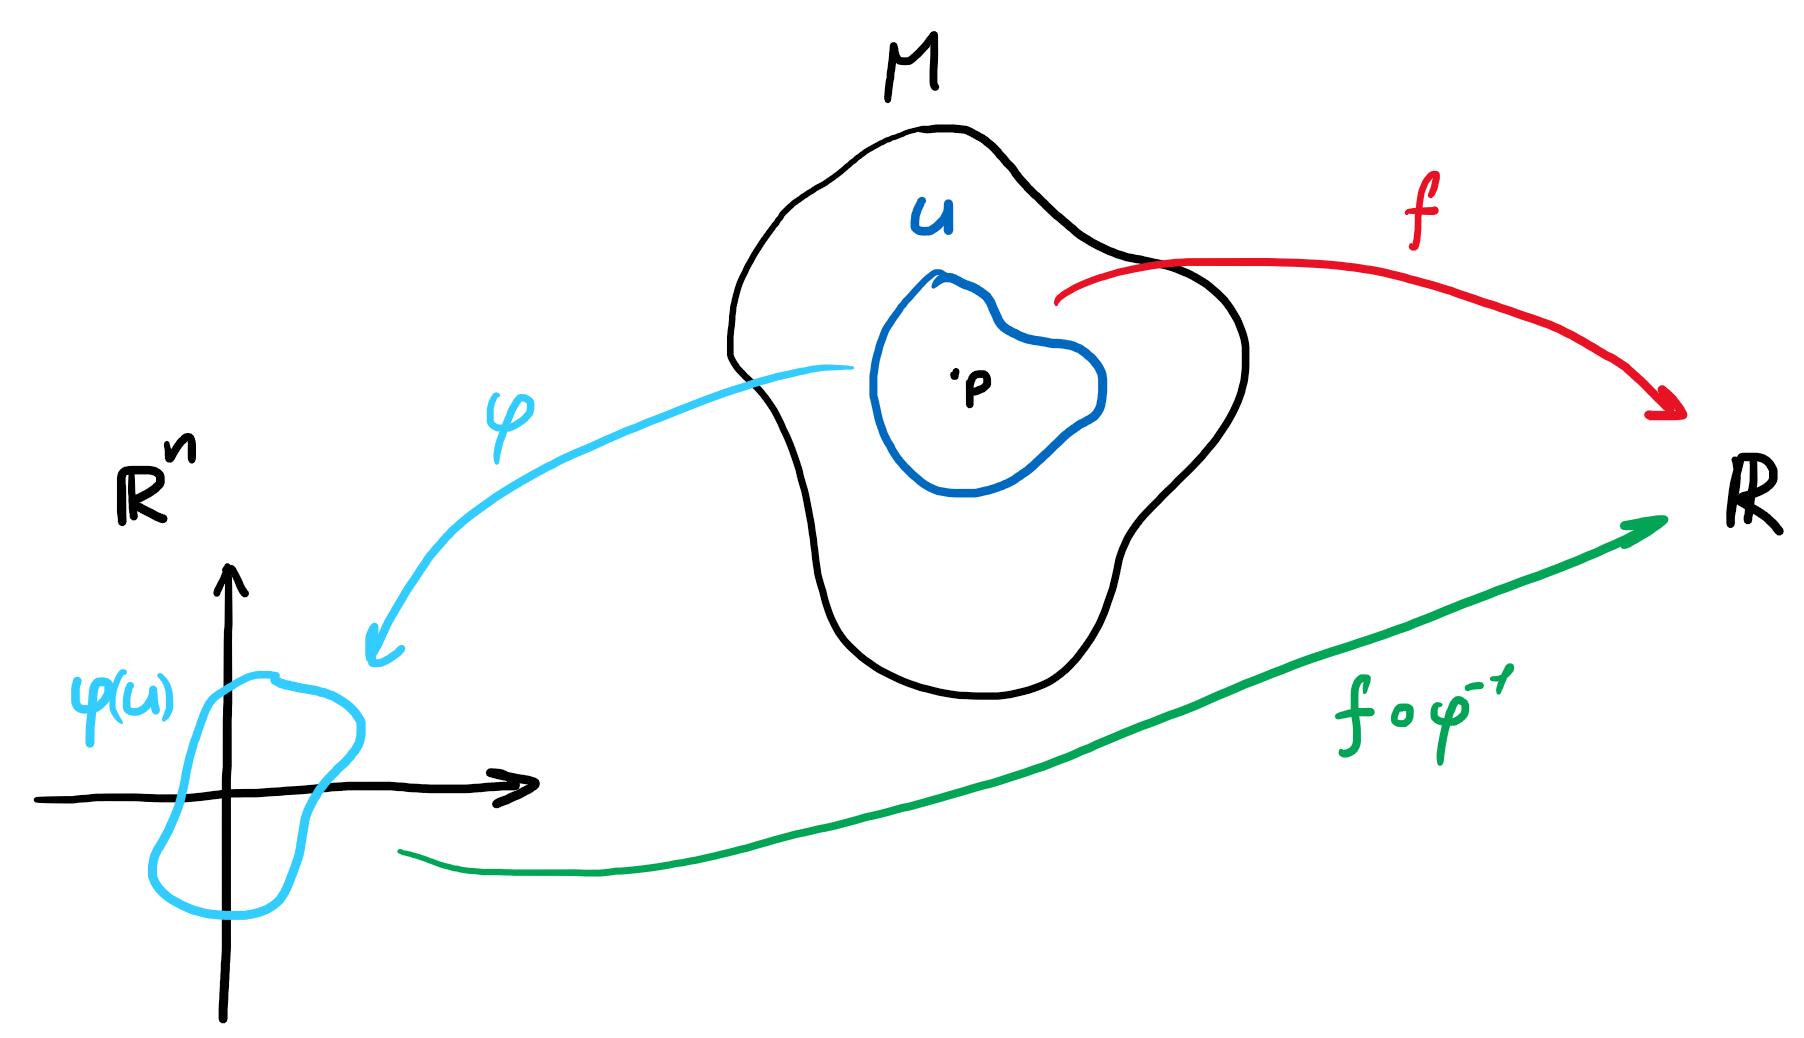
\includegraphics[width=0.6\textwidth,keepaspectratio]{img19}
\end{figure}

\begin{remark}
	$ (U,\phi) $ è una carta nella struttura differenziabile di $ M $ (l'atlante è fissato).
\end{remark}

La definizione non dipende dalla carta scelta intorno al punto $ p $, infatti se $ (V,\psi) $ è un'altra carta intorno a $ p $, allora

\begin{equation}
	f \circ \psi^{-1} = \left. (f \circ \phi^{-1})(\phi \circ \psi^{-1}) \right|_{\psi(U \cap V)} : \psi(U \cap V) \to \R
\end{equation}

dove $ \phi \circ \psi^{-1} \in C^{\infty} $ perché le carte a cui appartengono sono $ C^{\infty} $-compatibili e $ f \circ \phi^{-1} \in C^{\infty} $ per ipotesi, dunque $ \left. (f \circ \phi^{-1})(\phi \circ \psi^{-1}) \right|_{\psi(U \cap V)} \in C^{\infty} $ anche se ristretta a $ \psi(U \cap V) \ni p $, in quanto basta far vedere che esista un aperto opportuno che contenga il punto in cui la funzione sia liscia (è una condizione locale).\\
Una funzione $ f : M \to \R $ è liscia se lo per ogni punto $ p \in M $.

\begin{remark}
	Se $ f : M \to \R $ è una funzione liscia allora $ f $ è continua. Infatti $ f_{|\phi(U)} = f \circ \phi^{-1} \circ \phi $ dove $ \phi $ è continua perché omeomorfismo e $ f \circ \phi^{-1} $ è continua in quanto liscia.
\end{remark}

Indicheremo con $ C^{\infty}(M) $ l'insieme delle funzioni $ f : M \to \R $ lisce su $ M $ mentre $ C^{0}(M) $ sono le funzioni continue.

\begin{definition}
	Sia $ M $ una varietà differenziabile con atlante massimale $ \mathfrak{M} $ e sia un atlante differenziabile $ \mathfrak{U} \subset \mathfrak{M} $, allora $ f : M \to \R $ è liscia se e solo se per qualunque carta $ (U,\phi) \in \mathfrak{U} $ si ha che $ f \circ \phi^{-1} : \phi(U) \to \R $ sia liscia.
\end{definition}

\begin{proof}[Dimostrazione ($ \implies $)]
	Se $ f \in C^{\infty}(M) $ allora esiste una carta $ (V,\psi) \in \mathfrak{M} $ dell'atlante massimale tale che $ f \circ \psi^{-1} : \psi(V) \to \R $ sia liscia in $ p $: siccome la definizione di funzione liscia non dipende dalla carta scelta all'interno della struttura differenziabile, possiamo prendere anche la carta $ (U,\phi) \in \mathfrak{U} $ e dunque $ f \circ \phi^{-1} : \phi(U) \to \R $ è ancora liscia.
\end{proof}

\begin{proof}[Dimostrazione ($ \impliedby $)]
	Siccome gli insiemi delle carte dell'atlante $ \mathfrak{U} $ sono un ricoprimento di $ M $, prendendo il punto $ p \in M $, esisterà una carta $ (U,\phi) \ni p $ dell'atlante tale che, per ipotesi, $ f \circ \phi^{-1} : \phi(U) \to \R $ sia liscia, dunque abbiamo trovato una carta in cui è liscia perciò $ f $ è liscia in $ p $.
\end{proof}

Riassumendo, presa una varietà differenziabile $ M $ e un atlante differenziabile arbitrario $ \mathfrak{U} \subset \mathfrak{M} $ contenuto nella struttura differenziabile, allora $ f : M \to \R $ è liscia se e solo se per ogni carta $ (U,\phi) \in \mathfrak{U} $ abbiamo che $ f \circ \phi^{-1} : \phi(U) \to \R $ sia liscia.

\subsection{Funzioni lisce tra varietà}

Sia $ F : N \to M $ una funzione tra varietà differenziabili $ N $ e $ M $ di dimensione rispettivamente $ n $ e $ m $. Diremo che la funzione è $ C^{\infty} $ (liscia o differenziabile) in un punto $ p \in N $ se $ F $ è continua ed esiste una carta $ (U,\phi) $ di $ N $ intorno a $ p $ e una carta $ (V,\psi) $ di $ M $ intorno a $ F(p) $ tale che la composizione

\begin{equation}
	\psi \circ F_{|U} \circ \phi^{-1} : \phi(F^{-1}(V) \cap U) \to \R^{m}
\end{equation}

con $ \phi(F^{-1}(V) \cap U) \subset \R^{n} $, sia liscia in $ \phi(p) $\footnote{%
	$ F_{|U} \equiv F $ in quanto agisce prima $ \phi^{-1} $ che restringe già il dominio all'aperto $ U $.%
}.\\
Siccome non possiamo sapere se $ F(U) \subset V $, consideriamo l'aperto (in quanto $ F $ è continua) $ F^{-1}(V) \cap U \subset U $

\begin{figure}[H]
	\centering
	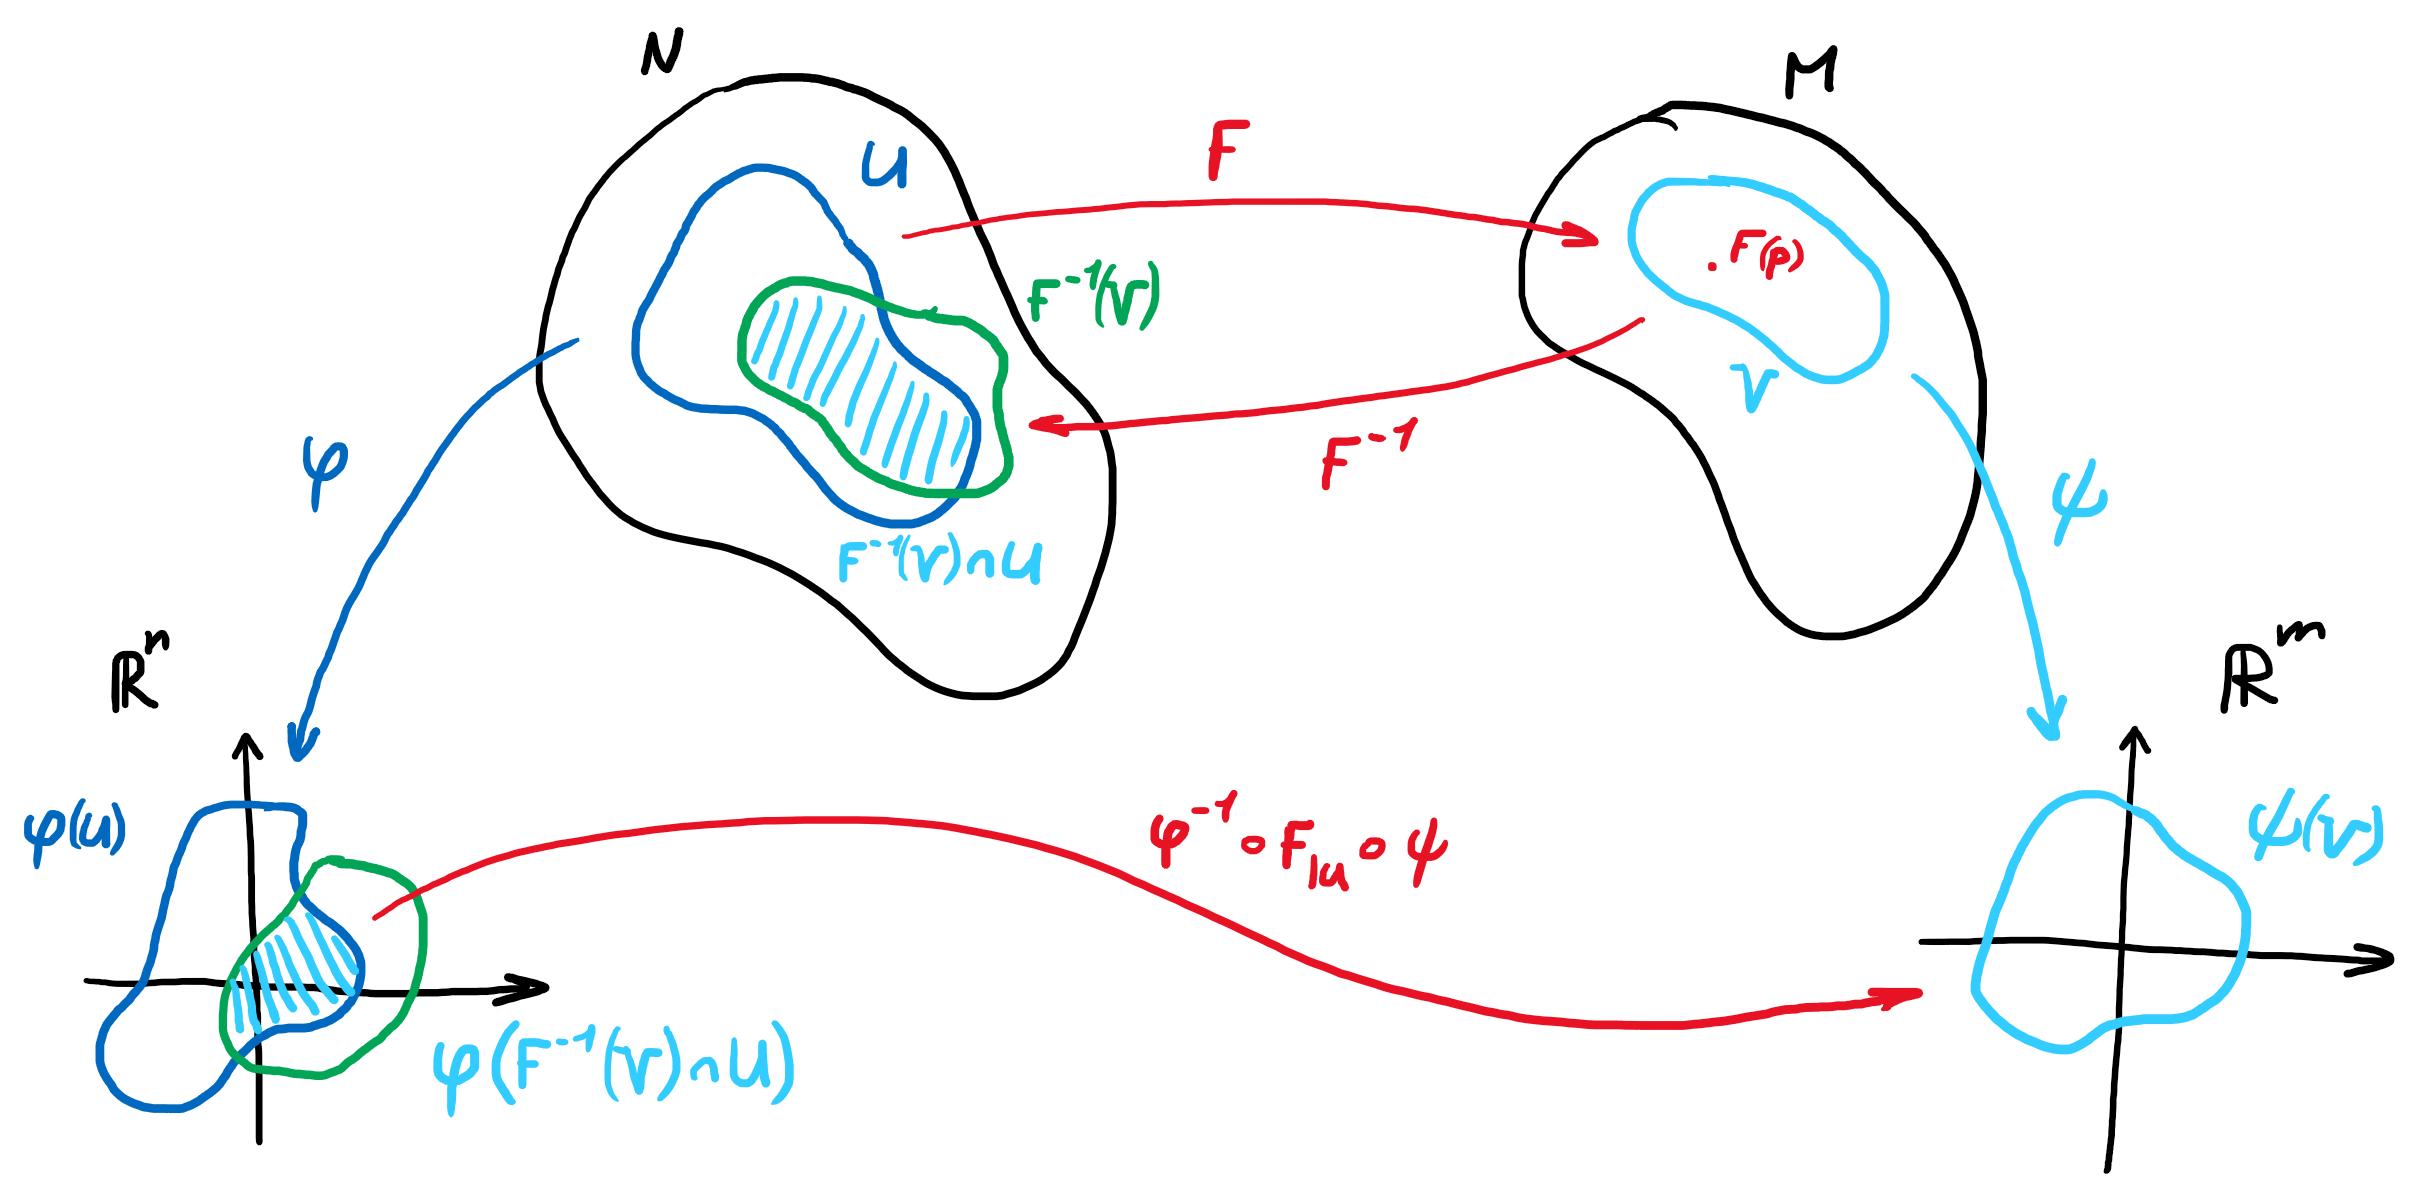
\includegraphics[width=0.85\textwidth,keepaspectratio]{img20}
\end{figure}

La definizione non dipende dalle carte scelte, infatti se $ (U',\phi') $ è una carta di $ N $ intorno a $ p $ e $ (V',\psi') $ è una carta di $ M $ intorno a $ F(p) $, allora

\begin{equation}
	\psi' \circ F \circ (\phi')^{-1} = \left. [(\psi' \circ \psi^{-1}) \circ (\psi \circ F \circ \phi^{-1}) \circ (\phi \circ (\phi')^{-1})] \right|_{\phi'(F^{-1}(V \cap V') \cap U \cap U')}
\end{equation}

dove $ \phi'(F^{-1}(V \cap V') \cap U \cap U') \ni \phi'(p) $, è liscia perché lo è $ \psi \circ F \circ \phi^{-1} $ per ipotesi e lo sono $ \psi' \circ \psi^{-1} $ e $ \phi \circ (\phi')^{-1} $ perché sono coppie di carte di una struttura differenziabile.\\
Una funzione $ F : N \to M $ è liscia se lo è in ogni punto $ p \in N $.

\begin{remark}
	Nel caso in cui lo spazio ambiente sia tutto $ \R^{n} $, i.e. $ F : N \to \R^{n} $, dove la struttura differenziale dello spazio euclideo $ \R^{n} $ è data dall'atlante massimale che contiene $ (\R^{n},\id_{\R^{n}}) $, la funzione $ F $ è liscia in $ p $ se e solo se l'applicazione
	
	\begin{equation}
		\id_{\R^{n}} \circ F \circ \phi^{-1} = F \circ \phi^{-1} : \phi(U) \to \R^{n}
	\end{equation}

	è liscia.\\
	Per $ n=1 $, questa è la definizione di funzione $ C^{\infty}(N) $.
\end{remark}

\begin{definition}
	Siano $ N $ e $ M $ varietà differenziabili, di dimensione rispettivamente $ n $ e $ m $, con strutture differenziabili $ \mathfrak{N} $ e $ \mathfrak{M} $ rispettivamente e siano $ \mathfrak{U} \subset \mathfrak{M} $ e $ \mathfrak{V} \subset \mathfrak{N} $ due strutture differenziali in N e M. Sia $ F : N \to M $ un'applicazione, allora $ F \in C^{\infty} $ in $ p $ se e solo se $ F $ è continua e si ha che
	
	\begin{equation}
		\psi' \circ F \circ (\phi')^{-1} : \phi'(F^{-1}(V') \cap U') \to \R^{m} \qcomma \forall (U',\phi') \in \mathfrak{U}, \forall (V',\psi') \in \mathfrak{V}
	\end{equation}

	sia liscia in $ \phi'(p) \in \phi'(F^{-1}(V') \cap U') $.
\end{definition}

\begin{proof}[Dimostrazione ($ \implies $)]
	Sia $ F \in C^{\infty}(M) $ e $ p \in N $, allora esistono delle carte $ p \in (U,\phi) \in \mathfrak{M} $ e $ F(p) \in (V,\psi) \in \mathfrak{N} $ tali che $ \psi \circ F \circ \phi^{-1} $ sia liscia in $ \phi(p) $. Ma, dato che la definizione della proprietà di essere liscia non dipende dalle carte scelte, questo significa che $ \psi' \circ F \circ (\phi')^{-1} $ è liscia in $ \phi'(p) $. La dimostrazione si conclude per il fatto che $ p $ sia arbitrario.
\end{proof}

\begin{proof}[Dimostrazione ($ \impliedby $)]
	La dimostrazione dell'implicazione inversa è immediata in quanto le carte degli atlanti sono un ricoprimento degli spazi.
\end{proof}

\begin{definition}[Composizione di funzioni lisce tra varietà]
	Siano $ M $, $ N $ e $ P $ varietà differenziabili ed $ F : N \to M $ e $ G : M \to P $ due funzioni continue e lisce, allora la composizione continua $ G \circ F $ è liscia.
\end{definition}

\begin{proof}
	Siano $ (U,\phi) $ una carta di $ N $ intorno a $ p \in N $ e $ (W,\sigma) $ una carta di $ P $ intorno a $ G(F(p)) $. Dobbiamo dimostrare che la funzione $ \sigma \circ G \circ F \circ \phi^{-1} $ sia liscia nel punto
	
	\begin{equation}
		\phi(p) \in \phi((G \circ F)^{-1}(W) \cap U) = \phi(F^{-1}(G^{-1}(W)) \cap U)
	\end{equation}
	
	Sia $ (V,\psi) $ una carta intorno a $ F(p) $, allora consideriamo la funzione
	
	\begin{equation}
		(\sigma \circ G \circ \psi) \circ (\psi^{-1} \circ F \circ \phi^{-1}) = \sigma \circ G \circ F \circ \phi^{-1}
	\end{equation}

	la quale è liscia, in quanto composizione di applicazioni lisce (i.e. $ \sigma \circ G \circ \psi $ e $ \psi^{-1} \circ F \circ \phi^{-1} $), in $ \phi(F^{-1}(G^{-1}(W) \cap V) \cap U) \ni \phi(p) $.
\end{proof}

\begin{definition}[Componenti]\label{map-comp}
	Sia un'applicazione $ F : N \to \R^{n} $ e sia la proiezione
	
	\begin{align}
		\begin{split}
			r^{i} : \R^{n} &\to \R\\
			(x^{1},\dots,x^{n}) &\mapsto x^{i}
		\end{split}
	\end{align}

	con $ i=1,\dots,n $.\\
	$ F $ è liscia se e solo se $ r^{i} \circ F \doteq F^{i} $ è liscia.
\end{definition}

\begin{proof}[Dimostrazione ($ \implies $)]
	Se $ F $ è liscia allora tutte le sue componenti $ F^{i} $ lo sono.
\end{proof}

\begin{proof}[Dimostrazione ($ \impliedby $)]
	Supponiamo che $ r^{i} \circ F \doteq F^{i} : N \to \R $ sia liscia per $ \forall i=1,\dots,n $. Per $ \forall p \in N $ abbiamo che $ F^{i} \circ \phi^{-1} : \phi(U) \to \R $ è liscia se scegliamo una carta $ (U,\phi) \ni p $, dove $ \phi(p) \subset \R^{n} $. A questo punto, la funzione
	
	\begin{align}
		\begin{split}
			F \circ \phi^{-1} : \phi(U) &\to \R^{n}\\
			q &\mapsto (F^{1} \circ \phi^{-1},\dots,F^{n} \circ \phi^{-1})(q)
		\end{split}
	\end{align}

	è liscia in $ \phi(p) $, dunque $ F $ è liscia in $ p $ per definizione, perché $ F \circ \phi^{-1} \equiv \id_{\R^{n}} \circ F \circ \phi^{-1} $.
\end{proof}

Riassumendo, prese due varietà differenziabili $ N $ ed $ M $ e due atlanti differenziabili arbitrari $ \mathfrak{U} \subset \mathfrak{N} $ e $ \mathfrak{V} \subset \mathfrak{M} $ contenuti nelle rispettive strutture differenziabili, allora $ F : N \to M $ è liscia se e solo se $ F $ è continua e per $ \forall (U,\phi) \in \mathfrak{U} $ e $ \forall (V,\psi) \in \mathfrak{V} $ abbiamo che $ \psi \circ F \circ \phi^{-1} : \phi(F^{-1}(V) \cap U) \to \R^{m} $ sia liscia.

\subsubsection{\textit{Esempio}}

Consideriamo l'applicazione continua

\begin{align}
	\begin{split}
		F  : \R &\to \S^{1}\\
		t &\mapsto (\cos 2 \pi t, \sin 2 \pi t)
	\end{split}
\end{align}

dove con $ \R $ e $ \S^{1} $ si intendono gli spazi con le loro strutture differenziabili fissate.\\
Fissiamo gli atlanti $ (\R,\id_{\R}) $ e $ \{(U_{i},\phi_{i})\}_{i=1,\dots,4} $ dove gli $ U_{i} $ sono le varie semicirconferenze di $ \S^{1} $ e le $ \phi_{i} $ sono le proiezioni di queste sugli assi\footnote{%
	Vedi Esempio \ref{ex-s1} per dettagli.%
}, i.e.

\begin{align}
	\begin{split}
		U_{1} &= \{ (x,y) \in \S^{1} \mid y>0 \}\\
		U_{2} &= \{ (x,y) \in \S^{1} \mid y<0 \}\\
		U_{3} &= \{ (x,y) \in \S^{1} \mid x>0 \}\\
		U_{4} &= \{ (x,y) \in \S^{1} \mid x<0 \}
	\end{split}	
\end{align}

\begin{align}
	\begin{split}
		\phi_{1} : U_{1} &\to (-1,1)_{x} \subset \R^{2}\\
		(x,y) &\mapsto x\\\\
		%
		\phi_{2} : U_{2} &\to (-1,1)_{x} \subset \R^{2}\\
		(x,y) &\mapsto x\\\\
		%
		\phi_{3} : U_{3} &\to (-1,1)_{y} \subset \R^{2}\\
		(x,y) &\mapsto y\\\\
		%
		\phi_{4} : U_{4} &\to (-1,1)_{y} \subset \R^{2}\\
		(x,y) &\mapsto y
	\end{split}
\end{align}

Dobbiamo verificare che l'applicazione $ \phi_{i} \circ F \circ \id_{\R} $ sia liscia per $ \forall i=1,\dots,4 $: innanzitutto $ \phi(F^{-1}(V) \cap U) $ della definizione corrisponde a $ \id_{\R}(F^{-1}(U_{i}) \cap \R) = F^{-1}(U_{i}) \subset \R $, dunque

\begin{align}
	\begin{split}
		\phi_{1} \circ F : F^{-1}(U_{1}) &\to \R^{2}\\
		t &\mapsto \cos 2 \pi t\\\\
		%
		\phi_{2} \circ F : F^{-1}(U_{2}) &\to \R^{2}\\
		t &\mapsto \cos 2 \pi t\\\\
		%
		\phi_{3} \circ F : F^{-1}(U_{3}) &\to \R^{2}\\
		t &\mapsto \sin 2 \pi t\\\\
		%
		\phi_{4} \circ F : F^{-1}(U_{4}) &\to \R^{2}\\
		t &\mapsto \sin 2 \pi t
	\end{split}
\end{align}

le quali sono tutte lisce perciò lo è anche $ F $.

\subsection{Diffeomorfismi tra varietà}

Siano $ N $ e $ M $ due varietà differenziabili, un'applicazione $ F : N \to M $ è un \textit{diffeomorfismo} se

\begin{itemize}
	\item $ F $ è invertibile
	
	\item $ F \in C^{\infty} $
	
	\item $ F^{-1} \in C^{\infty} $
\end{itemize}

Diremo che due varietà $ N $ e $ M $ sono \textit{diffeomorfe} se esiste un diffeomorfismo $ F : N \to M $ che le collega; se due varietà $ N $ e $ M $ sono diffeomorfe, scriveremo $ M \simeq N $.\\
Sia $ V $ la classe di tutte le varietà differenziabili, allora

\begin{equation}
	M \sim N \iff M \simeq N
\end{equation}

definisce una relazione di equivalenza su $ V $.

\begin{theorem}
	Una varietà differenziabile di dimensione 1 connessa (curva differenziabili) è diffeomorfa ad $ \S^{1} $ (compatta) oppure ad $ \R $ (non compatta).
\end{theorem}

\begin{theorem}
	Se $ N $ è una superficie differenziabile (varietà differenziabile di dimensione 2) compatta e connessa allora $ N $ è diffeomorfa a $ \Sigma_{g} $, cioè una superficie con $ g $ \textit{buchi}. Questa superficie è una generalizzazione del toro (il quale ha un solo buco).
	
	\begin{figure}[H]
		\centering
		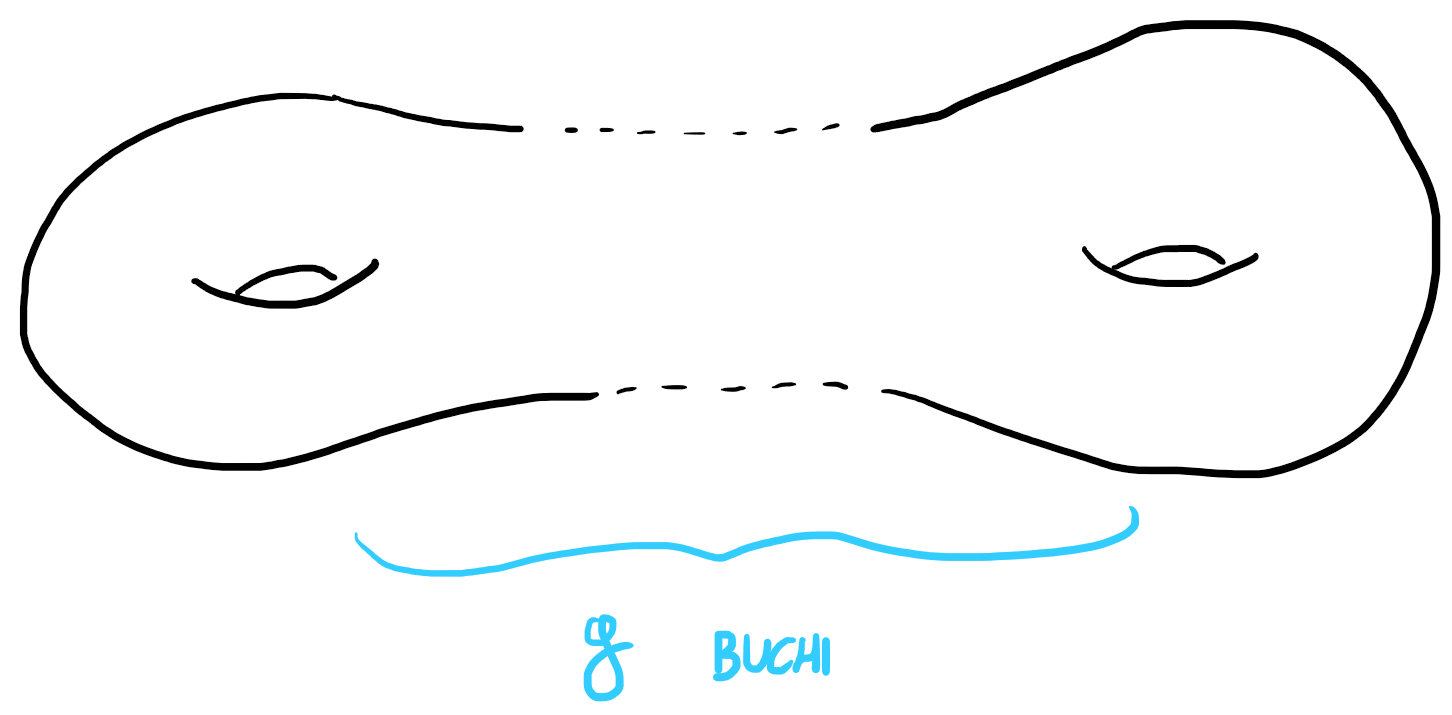
\includegraphics[width=0.3\textwidth,keepaspectratio]{img21}
	\end{figure}
\end{theorem}

\begin{remark}
	Non ha senso classificare le superfici non compatte in quanto ogni spazio $ \R^{2} \setminus U $ con $ U $ chiuso in $ \R^{2} $ è una varietà differenziabile e i chiusi non sono classificabili.
\end{remark}

Data una varietà topologica $ M $, vogliamo ora determinare quante strutture differenziabili siano compatibili con $ M $ a meno di diffeomorfismi:

\begin{itemize}
	\item Se $ \dim(M) < 4 $ allora esiste una sola struttura differenziale su $ M $
	
	\item Se $ \dim(M) > 4 $ allora esiste un numero finito di strutture differenziabili su $ M $ (a meno di diffeomorfismi)
\end{itemize}

Ad esempio, sull'ipersfera $ \S^{7} $ esistono 28 strutture differenziabili non diffeomorfe tra loro.

\begin{remark}
	Non si sa se su $ \S^{4} $ esista un numero finito o infinito di strutture differenziabili.
\end{remark}

\begin{remark}
	Esistono varietà topologiche che non ammettono strutture differenziabili.
\end{remark}

\subsubsection{\textit{Esempi}}

\paragraph{1.}

Sia $ \R $ la varietà differenziabile con atlante $ (\R,\id_{\R}) $ e $ \R' $ la stessa varietà topologica con atlante differenziabile $ (\R,\psi) $, dove

\begin{align}
	\begin{split}
		\psi : \R &\to \R\\
		x &\mapsto x^{\sfrac{1}{3}}
	\end{split}	
\end{align}

Queste due strutture differenziali sono diverse, cioè le loro carte non sono $ C^{\infty} $-compatibili, infatti il cambio di carta $ \psi \circ (\id_{\R})^{-1} = \psi $ non è liscio, però sono diffeomorfe tramite l'applicazione

\begin{align}
	\begin{split}
		F : \R &\to \R'\\
		x &\mapsto x^{3}
	\end{split}	
\end{align}

con inversa

\begin{align}
	\begin{split}
		F^{-1} : \R' &\to \R\\
		x &\mapsto x^{\sfrac{1}{3}}
	\end{split}	
\end{align}

la quale è un diffeomorfismo perché continua e liscia. Per dimostrare che $ F \in C^{\infty} $, controlliamo la composizione tra carte

\begin{align}
	\begin{split}
		\psi \circ F \circ (\id_{\R})^{-1} = \psi \circ F = \id_{\R} : \R &\to \R\\
		x &\mapsto x\\\\
		%
		\id_{\R} \circ F^{-1} \circ \psi^{-1} = F^{-1} \circ \psi^{-1} = \id_{\R} : \R' &\to \R'\\
		x &\mapsto x
	\end{split}	
\end{align}

le quali sono entrambe lisce.\\
L'identità da $ \R $ in $ \R' $ non è un diffeomorfismo in quanto

\begin{align}
	\begin{split}
		(\psi \circ \id \circ (\id_{\R})^{-1})(x) &= \psi(x)\\
		&= x^{\sfrac{1}{3}}
	\end{split}
\end{align}

non è liscia.

\paragraph{2.}

Nonostante sia controintuitivo, possiamo considerare il cerchio unitario $ \S^{1} $ come una varietà topologica di dimensione\footnote{%
	Numero arbitrario.%
} 307 non compatta: oltre alla topologia considerata in precedenza (quella che viene normalmente chiamata "standard"), $ \S^{1} $ è in bigezione con $ \R^{307} $, dunque possiamo portare la struttura di varietà topologica standard di $ \R^{307} $ in $ \S^{1} $ ($ \R^{307} $ non è compatto quindi non lo sarà nemmeno $ \S^{1} $).\\
Lo stesso discorso vale se consideriamo la proprietà di varietà differenziale.

\subsection{Carte e diffeomorfismi}

\begin{definition}
	Sia $ N $ una varietà differenziabile e $ (U,\phi) $ una sua carta, allora l'applicazione $ \phi : U \to \phi(U) $ è un diffeomorfismo, dove la struttura differenziabile di $ U $ proviene da quella di $ N $ mentre quella di $ \phi(U) $ da $ \R^{n} $.
\end{definition}

\begin{proof}
	Osserviamo che $ (U,\phi) $ è un'atlante differenziabile per $ U $ e $ (\phi(U),\id_{\R^{n}}) $ è un atlante differenziabile per $ \phi(U) $, allora per la definizione di funzione liscia tra varietà
	
	\begin{align}
		\begin{split}
			\id_{\phi(U)} \circ \phi \circ \phi^{-1} &= \id_{\phi(U)}\\
			\phi \circ \phi^{-1} \circ \id_{U} &= \id_{U}
		\end{split}	
	\end{align}

	abbiamo che $ \phi $ è un diffeomorfismo tra $ U $ e $ \phi(U) $.
\end{proof}

\begin{definition}\label{diffeo-map}
	Sia $ U \subset N $ un aperto di una varietà differenziabile $ N $ di dimensione $ n $ e sia $ F : U \to F(U) \subset \R^{n} $ (aperto) un diffeomorfismo, allora $ (U,F) $ è una carta di $ N $ (nella struttura differenziabile di $ N $).
\end{definition}

\begin{proof}
	\`{E} sufficiente verificare che $ (U,F) $ sia compatibile con ogni carta $ (U_{\alpha},\phi_{\alpha}) $ dell'atlante massimale $ \mathfrak{N} $ di $ N $ che definisce la sua struttura differenziabile, cioè appartiene all'atlante stesso.\\
	Prendiamo i cambi di carte
	
	\begin{align}
		\begin{split}
			F \circ (\phi_{\alpha})^{-1} : \phi_{\alpha}(U_{\alpha} \cap U) \to F(U_{\alpha} \cap U)\\
			\phi_{\alpha} \circ F^{-1} : F(U_{\alpha} \cap U) \to \phi_{\alpha}(U_{\alpha} \cap U)
		\end{split}	
	\end{align}

	in cui $ F $ è liscia in quanto diffeomorfismo e $ \phi_{\alpha} $ e la sua inversa sono lisce per la dimostrazione precedente, perciò i cambi di carte sono anch'essi lisci in quanto composizione di applicazioni lisce.
\end{proof}

\subsection{Proiezioni tra varietà}

Siano $ N $ e $ M $ due varietà differenziabili di dimensione $ n $ e $ m $ rispettivamente e siano le proiezioni

\begin{align}
	\begin{split}
		\pi_{N} : N \times M &\to N\\
		(x,y) &\mapsto x\\\\
		%
		\pi_{M} : N \times M &\to M\\
		(x,y) &\mapsto y
	\end{split}	
\end{align}

allora $ \pi_{N} $ e $ \pi_{M} $ sono lisce.\\
Sia $ \{(U_{\alpha},\phi_{\alpha})\}_{\alpha \in A} $ un atlante differenziabile per $ N $ e $ \{(V_{\beta},\psi_{\beta})\}_{\beta \in B} $ un atlante differenziabile per $ M $, dunque $ \{(U_{\alpha} \times V_{\beta},\phi_{\alpha} \times \psi_{\beta})\} $ è un atlante differenziabile per $ N \times M $. Per far vedere che $ \pi_{N} $ sia liscia (la dimostrazione per $ \pi_{M} $ è analoga), siccome per la teoria $ F : N \to M $ con la verifica

\begin{equation}
	\psi \circ F \circ \phi^{-1} : \phi(F^{-1}(V) \cap U) \to \R^{n}
\end{equation}

allora il dominio è

\begin{align}
	\begin{split}
		(\phi_{\alpha} \times \psi_{\beta})(\pi^{-1}(U_{\alpha}) \cap (U_{\alpha} \times V_{\beta})) &= (\phi_{\alpha} \times \psi_{\beta})((U_{\alpha} \times M) \cap (U_{\alpha} \times V_{\beta}))\\
		&= (\phi_{\alpha} \times \psi_{\beta})(U_{\alpha} \times V_{\beta})\\
		&= \phi_{\alpha}(U_{\alpha}) \times \psi_{\beta}(V_{\beta})
	\end{split}	
\end{align}

dove $ \phi_{\alpha}(U_{\alpha}) \subset \R^{n} $ e $ \psi_{\beta}(V_{\beta}) \subset \R^{m} $, perciò

\begin{align}
	\begin{split}
		\phi_{\alpha} \circ \pi_{N} \circ (\phi_{\alpha} \times \psi_{\beta})^{-1} : \phi_{\alpha}(U_{\alpha}) \times \psi_{\beta}(V_{\beta}) &\to \R^{n}\\
		(a^{1},\dots,a^{n},b^{1},\dots,b^{m}) &\mapsto \phi_{\alpha} (\pi_{N} ((\phi_{\alpha}^{-1} \times \psi_{\beta}^{-1}) ((a^{1},\dots,a^{n},b^{1},\dots,b^{m}))))\\
		&\mapsto \phi_{\alpha} (\pi_{N} ((\phi_{\alpha}^{-1}((a^{1},\dots,a^{n})),\psi_{\beta}^{-1}((b^{1},\dots,b^{m}))))\\
		&\mapsto \phi_{\alpha} (\phi_{\alpha}^{-1}((a^{1},\dots,a^{n})))\\
		&\mapsto (a^{1},\dots,a^{n})
	\end{split}	
\end{align}

i.e. $ \phi_{\alpha} \circ \pi_{N} \circ (\phi_{\alpha} \times \psi_{\beta})^{-1} \equiv \pi_{N} $, la quale è liscia.\\\\
%
Siano $ N $, $ M_{1} $ e $ M_{2} $ tre varietà differenziabili e sia l'applicazione

\begin{align}
	\begin{split}
		F : N &\to M_{1} \times M_{2}\\
		q &\mapsto (F_{1}(q),F_{2}(q))
	\end{split}
\end{align}

dove $ F_{1} : N \to M_{1} $ e $ F_{1} : N \to M_{2} $, allora $ F $ è liscia se e solo se lo sono $ F_{1} $ e $ F_{2} $.\\
Infatti, se $ F $ è liscia allora le sue componenti $ F_{i} = \pi_{i} \circ F $ (con $ \pi_{i} : M_{1} \times M_{2} \to M_{i} $) devono essere lisce: questo è verificato perché $ \pi_{i} \in C^{\infty} $ per $ i=1,2 $, dunque la composizione che risulta in $ F_{i} $ è liscia.\\
Viceversa, se $ F_{1} $ e $ F_{2} $ sono lisce allora $ \phi_{1} \circ F_{1} \circ \phi^{-1} $ e $ \phi_{2} \circ F_{2} \circ \phi^{-1} $ sono lisce, dove $ (U_{1},\phi_{1}) $ è una carta in $ M_{1} $, $ (U_{2},\phi_{2}) $ è una carta in $ M_{2} $ e $ (U,\phi) $ è una carta in $ N $. A questo punto

\begin{equation}
	(\phi_{1} \circ F_{1} \circ \phi^{-1}, \phi_{2} \circ F_{2} \circ \phi^{-1}) = (\phi_{1} \times \phi_{2}) \circ F \circ \phi^{-1}
\end{equation}

è liscia e, per definizione di applicazione liscia, lo è anche $ F $.

\subsection{Gruppi di Lie}

Un \textit{gruppo di Lie} $ G $ è un gruppo algebrico che sia anche una varietà differenziabile con le operazioni di gruppo lisce, i.e. le operazioni

\begin{align}
	\begin{split}
		\mu : G \times G &\to G\\
		(g,h) &\mapsto g \cdot h\\\\
		%
		i : G &\to G\\
		g &\mapsto g^{-1}
	\end{split}
\end{align}

sono lisce.

\subsubsection{\textit{Esempi}}

\paragraph{1. $ \R $ e somma}

Il gruppo $ (\R,+) $ è anche una varietà differenziabile. Le operazioni

\begin{align}
	\begin{split}
		+ : \R \times \R &\to \R\\
		(x,y) &\mapsto x+y\\\\
		%
		i : \R &\to \R\\
		x &\mapsto - x
	\end{split}
\end{align}

sono lisce dunque è un gruppo di Lie.

\paragraph{2. $ \R \setminus \{0\} $ e prodotto}

Il gruppo $ (\R \setminus \{0\},\cdot) $ è una varietà differenziabile e dunque gruppo di Lie in quanto

\begin{align}
	\begin{split}
		\cdot : \R \setminus \{0\} \times \R \setminus \{0\} &\to \R \setminus \{0\}\\
		(x,y) &\mapsto x \cdot y\\\\
		%
		i : \R &\to \R\\
		x &\mapsto x^{-1}
	\end{split}
\end{align}

sono lisce.

\paragraph{3. Cerchio unitario $ \S^{1} $}

Il cerchio unitario

\begin{equation}
	\S^{1} = \{ z \in \C \, \mid \, \norm{z} = 1 \} \subset \C
\end{equation}

dove $ \C $ indica l'insieme dei numeri complessi, è un gruppo di Lie in quanto

\begin{align}
	\begin{split}
		\cdot : \S^{1} \times \S^{1} &\to \S^{1}\\
		(z,w) &\mapsto z \cdot w\\\\
		%
		i : \S^{1} &\to \S^{1}\\
		z &\mapsto z^{-1}
	\end{split}
\end{align}

sono lisce.

\paragraph{4. Prodotto diretto}

Il prodotto diretto di gruppi di Lie è ancora un gruppo di Lie, con il prodotto tra varietà differenziabili e con l'operazione componente per componente.\\
Vedi Esercizio \ref{es3-1}.

\paragraph{5. $ GL_{n}(\R) $}

Il gruppo delle matrici invertibili

\begin{equation}
	GL_{n}(\R) = \{ A \in M_{n}(\R) \, \mid \, \det(A) \neq 0 \} \subset M_{n}(\R) = \R^{n^{2}}
\end{equation}

con la struttura differenziale è ereditata da $ M_{n}(\R) = \R^{n^{2}} $, in quanto $ GL_{n}(\R) $ è aperto in questo spazio, è un gruppo di Lie rispetto alla moltiplicazione. La carta $ (GL_{n}(\R),\id) $ corrisponde ad un atlante per $ GL_{n}(\R) $.\\
Per dimostrare che sia un gruppo di Lie, dobbiamo verificare che le operazioni di moltiplicazione e di inversione siano lisce: consideriamo il prodotto tra matrici

\begin{align}
	\begin{split}
		\mu : GL_{n}(\R) \times GL_{n}(\R) &\to GL_{n}(\R)\\
		(A,B) &\mapsto A B
	\end{split}
\end{align}

se $ A = (a_{ij}) $ e $ B = (b_{jk}) $ allora

\begin{equation}
	(A B)_{ik} = \sum_{j=1}^{n} a_{ij} b_{jk}
\end{equation}

dunque $ \mu \in C^{\infty} $ in quanto somma e prodotto di funzioni lisce; l'inversione è definita come

\begin{align}
	\begin{split}
		i : GL_{n}(\R) &\to GL_{n}(\R)\\
		A &\mapsto A^{-1}
	\end{split}
\end{align}

considerando la matrice dei cofattori $ \mathcal{C} $

\begin{equation}
	\mathcal{C}_{ij} \doteq (-1)^{i+j} m_{ij} = (-1)^{i+j} \det(A_{ij})
\end{equation}

dove gli $ A_{i,j} $ sono le sottomatrici di $ A $ (le matrici a cui sono state tolte la riga $ i $ e la colonna $ j $), si ha che l'inverso di una matrice $ A $ è dato da

\begin{equation}
	A^{-1} = \dfrac{1}{\det(A)} \, \mathcal{C}^{T}
\end{equation}

dunque l'inversione è liscia in quanto composizione di funzioni lisce.

\subsection{Derivate parziali su varietà differenziabili}

Fissiamo una varietà differenziabile $ N $ di dimensione $ n $ e una carta $ (U,\phi) $ intorno ad un punto $ p $, dunque abbiamo il diffeomorfismo $ \phi : U \to \phi(U) \subset \R^{n} $. Prendendo la proiezione

\begin{align}
	\begin{split}
		r^{i} : \R^{n} &\to \R\\
		(x^{1},\dots,x^{n}) &\mapsto x^{i}
	\end{split}
\end{align}

con $ i=1,\dots,n $, otteniamo che $ x^{i} = r^{i} \circ \phi $, in quanto $ \phi(p) = (x^{1}(p),\dots,x^{n}(p)) \in \R^{n} $.\\
Consideriamo una funzione $ f : N \to \R $ che sia $ C^{\infty}(N) $, vogliamo definire la \textit{derivata parziale di} $ f $ \textit{rispetto alla coordinata} $ x^{i} $, i.e. $ \sfrac{\partial f}{\partial x^{i}} (p) $, la quale dipenderà dunque dalla carta scelta. L'idea alla base della derivata parziale di una funzione su una varietà è quella di riportare tutto ad $ \R^{n} $ e svolgere la derivata usuale, dunque definiamo

\begin{equation}
	\dfrac{\partial f}{\partial x^{i}} (p) \doteq \left. \dfrac{\partial}{\partial x^{i}} \right|_{p} f
\end{equation}

Usando la composizione $ f \circ \phi^{-1} : \phi(U) \to \R $

\begin{figure}[H]
	\centering
	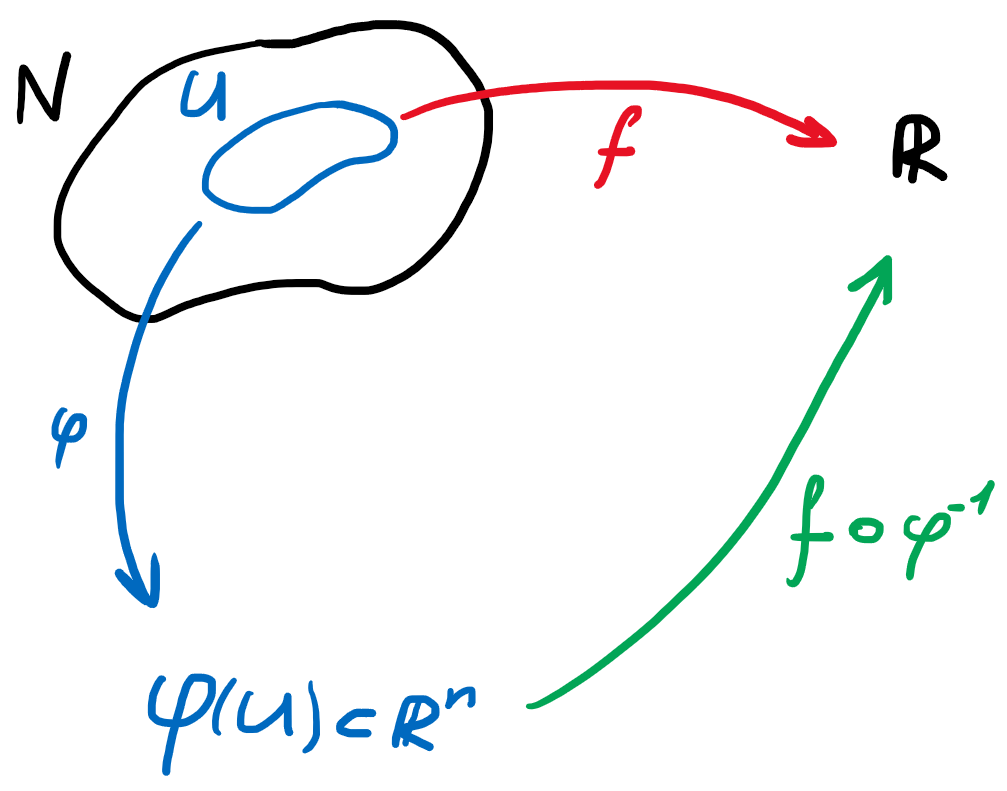
\includegraphics[width=0.4\textwidth,keepaspectratio]{img22}
\end{figure}

scriviamo

\begin{equation}
	\left. \dfrac{\partial}{\partial x^{i}} \right|_{p} f = \dfrac{\partial (f \circ \phi^{-1})}{\partial r^{i}} (\phi(p)) \doteq \left. \dfrac{\partial}{\partial r^{i}} \right|_{\phi(p)} (f \circ \phi^{-1})
\end{equation}

La dipendenza dalle carte scelte per la varietà è analoga alla scelta delle coordinate per $ \R^{n} $ (e.g. standard vs. polari).

\begin{definition}
	Presa una funzione $ f \in C^{\infty} $ su una varietà, la sua derivata parziale
	
	\begin{equation}
		\dfrac{\partial f}{\partial x^{i}} (p) \doteq \left. \dfrac{\partial}{\partial r^{i}} \right|_{\phi(p)} (f \circ \phi^{-1}) : U \to \R
	\end{equation}

	è ancora liscia.
\end{definition}

\begin{proof}
	Possiamo scrivere
	
	\begin{align}
		\begin{split}
			\dfrac{\partial f}{\partial x^{i}} (p) &= \dfrac{\partial f}{\partial x^{i}} (\phi^{-1}(\phi(p)))\\
			&\doteq \dfrac{\partial (f \circ \phi^{-1})}{\partial r^{i}} (\phi(p))
		\end{split}
	\end{align}

	a questo punto
	
	\begin{equation}
		\pdv{f}{x^{i}} \circ \phi^{-1} = \pdv{(f \circ \phi^{-1})}{r^{i}} \qcomma \forall i=1,\dots,n
	\end{equation}

	la quale è la derivata di una composizione di funzioni lisce, i.e. $ f \circ \phi^{-1} $. Deduciamo dunque che la derivata è liscia in quanto l'equazione sopra corrisponde alla definizione di funzione liscia su varietà.
\end{proof}

\subsubsection{\textit{Esempio}}

Sia $ N $ una varietà differenziabile e $ (U,\phi) $ con $ \phi = (x^{1},\dots,x^{n}) $ una carta.\\
Allora

\begin{equation}
	\dfrac{\partial x^{i}}{\partial x^{j}} = \delta^{ij}
\end{equation}

Infatti, usando la definizione

\begin{equation}
	\dfrac{\partial x^{i}}{\partial x^{j}} (p) = \dfrac{\partial (x^{i} \circ \phi^{-1})}{\partial r^{j}} (\phi(p))
\end{equation}

con $ p \in U $ e $ r^{j} $ le coordinate standard di $ \R^{n} $, siccome $ x^{i} = \phi \circ r^{i} $

\begin{align}
	\begin{split}
		\dfrac{\partial x^{i}}{\partial x^{j}} (p) &= \dfrac{\partial r^{i}}{\partial r^{j}} (\phi(p))\\
		&= \delta^{ij}
	\end{split}
\end{align}

\subsection{Jacobiano per applicazioni tra varietà}

Sia un'applicazione $ F : N \to M $ liscia con $ N $ e $ M $ varietà differenziabili con dimensioni $ n $ e $ m $ rispettivamente e fissiamo due carte $ (U,\phi) \in N $ e $ (V,\psi) \in M $, dove $ F(U) \subset V $ (è sempre possibile e inoltre non restrittivo in quanto è possibile prendere l'aperto $ U $ arbitrariamente piccolo affinché si verifichi questa condizione\footnote{%
	Qualunque aperto contenuto in una carta definisce ancora una carta nella struttura differenziabile: se $ U \subset U_{\alpha} $ dove $ (U_{\alpha},\phi_{\alpha}) $ è una carta della varietà differenziabile, allora $ (U, \phi_{\alpha \mid U}) $ è ancora una carta della stessa varietà.%
}).\\
Sia la componente $ i $-esima di $ F $ rispetto alle coordinate $ (y^{1},\dots,y^{m}) $

\begin{equation}
	F^{i} = y^{i} \circ F = r^{i} \circ \psi \circ F \qcomma i=1,\dots,m
\end{equation}

dove $ \psi = (y^{1},\dots,y^{m}) $. L'applicazione $ F^{i} : U \to \R $ è $ C^{\infty}(U) $, quindi possiamo definire le sue derivate parziali

\begin{equation}
	\dfrac{\partial F^{i}}{\partial x^{j}} : U \to \R
\end{equation}

le quali possono essere organizzate nella \textit{matrice jacobiana} $ J $ \textit{di} $ F $ rispetto alle carte $ (U,\phi) $ e $ (V,\psi) $ nel punto $ p \in U $

\begin{align}
	\begin{split}
		J(F) &\doteq \left[ \dfrac{\partial F^{i}}{\partial x^{j}} (p) \right] \in M_{m,n}(\R)\\\\
		&= \begin{bmatrix} \dfrac{\partial F^{1}}{\partial x^{1}} (p) & & \cdots & & \dfrac{\partial F^{1}}{\partial x^{m}} (p) \\\\ \vdots & & \ddots & & \vdots \\\\ \dfrac{\partial F^{n}}{\partial x^{1}} (p) & & \cdots & & \dfrac{\partial F^{n}}{\partial x^{m}} (p) \end{bmatrix}
	\end{split}
\end{align}

Quindi, per definizione di derivata parziale

\begin{equation}
	\dfrac{\partial F^{i}}{\partial x^{j}} (p) = \dfrac{\partial (F^{i} \circ \phi^{-1})}{\partial r^{j}} (\phi(p))
\end{equation}

Nel caso in cui $ N = \R^{n} $ e $ M = \R^{m} $

\begin{equation}
	\dfrac{\partial F}{\partial x^{i}} = \dfrac{\partial F}{\partial r^{i}}
\end{equation}

in quanto le carte hanno come applicazioni delle identità.\\
Se la dimensione della varietà di partenza è uguale alla dimensione della varietà di arrivo $ n=m $, allora $ J \in M_{n}(\R) $ e il suo determinante $ \det(J) $ si chiama \textit{determinante jacobiano}.

\subsubsection{Matrice jacobiana del cambio di coordinate}

Sia $ N $ una varietà differenziabile e siano $ (U,\phi) $ e $ (V,\psi) $ due carte di $ N $ con $ \phi = (x^{1},\dots,x^{n}) $ e $ \psi = (y^{1},\dots,y^{n}) $. Consideriamo il diffeomorfismo tra aperti di $ \R^{n} $

\begin{equation}
	\psi \circ \phi^{-1} : \phi(U \cap V) \to \psi(U \cap V)
\end{equation}

Possiamo quindi calcolare la sua matrice jacobiana, sapendo che le $ y^{i} : U \cap V \to \R $ sono lisce

\begin{align}
	\begin{split}
		J(\psi \circ \phi^{-1})(\phi(p)) &= \left[ \dfrac{\partial (\psi \circ \phi^{-1})^{i}}{\partial r^{j}} (\phi(p)) \right] \in M_{n}(\R)\\
		&= \left[ \dfrac{\partial y^{i}}{\partial x^{j}} (p) \right]
	\end{split}
\end{align}

perché, scrivendo esplicitamente le componenti, otteniamo

\begin{align}
	\begin{split}
		\dfrac{\partial (\psi \circ \phi^{-1})^{i}}{\partial r^{j}} (\phi(p)) &= \dfrac{\partial (r^{i} \circ \psi \circ \phi^{-1})}{\partial r^{j}} (\phi(p))\\
		&= \dfrac{\partial (y^{i} \circ \phi^{-1})}{\partial r^{j}} (\phi(p))\\
		&= \left( \dfrac{\partial y^{i}}{\partial r^{j}} \circ \phi^{-1} \right) (\phi(p))\\
		&= \dfrac{\partial y^{i}}{\partial x^{j}} (p)
	\end{split}
\end{align}

\subsection{Teorema della funzione inversa}

Sia $ F : N \to M $ un'applicazione liscia, diremo che $ F $ è un \textit{diffeomorfismo locale} in un punto $ p \in N $ se esiste un intorno $ U $ di $ p $ in $ N $ tale che $ F(U) \subset M $ sia aperto e $ F : U \to F(U) $ sia un diffeomorfismo.

\begin{theorem}[Teorema della funzione inversa (IFT) in analisi]
	Sia $ F : W \to \R^{n} $ con $ W \subset \R^{n} $ aperto e $ F \in C^{\infty} $, allora $ F $ è un diffeomorfismo locale in $ p \in W $ se e solo se lo jacobiano associato è invertibile, i.e.
	
	\begin{equation}
		\det(J(F)(p)) = \det( \left[ \pdv{F}{x^{j}} \hspace{0px} (p) \right] ) \neq 0
	\end{equation}
\end{theorem}

Possiamo quindi individuare un intorno $ U \subset W $ di un punto $ p $ il quale sia diffeomorfo alla sua immagine tramite $ F $ controllando semplicemente un numero, il quale dipende esclusivamente dal punto e non dal suo intorno.\\
Questo teorema implica un altro teorema

\begin{theorem}[IFT in geometria differenziale]\label{ift}
	Sia $ F : N \to M $ un'applicazione liscia dove $ \dim(N) = \dim(M) $ e sia un punto $ p \in N $, allora $ F $ è un diffeomorfismo locale in $ p $ se e solo se la matrice jacobiana per varietà è invertibile, i.e.
	
	\begin{equation}
		\det(J(F)(p)) = \det( \left[ \pdv{F}{x^{j}} \hspace{0px} (p) \right] ) \neq 0
	\end{equation}
	
	per carte $ (U,\phi) \in N $ e $ (V,\psi) \in M $ tale che $ F(U) \subseteq V $, dove $ p \in U $ e $ F(p) \in V $.
\end{theorem}

Questa estensione alle varietà è naturale in quanto possiamo scrivere l'applicazione tra varietà localmente come da un aperto di $ \R^{n} $ ad $ \R^{n} $ e quindi utilizzare il teorema della funzione inversa dell'analisi.

\begin{proof}
	Osserviamo che
	
	\begin{equation}
		J(\psi \circ F \circ \phi^{-1})(\phi(p)) = \left[ \dfrac{\partial F}{\partial x^{j}} (p) \right]
	\end{equation}

	in quanto, esattamente come per il cambio di carte
	
	\begin{align}
		\begin{split}
			J(\psi \circ F \circ \phi^{-1})(\phi(p)) &= \left[ \dfrac{\partial (\psi \circ F \circ \phi^{-1})^{i}}{\partial r^{j}} (\phi(p)) \right]\\
			&= \left[ \dfrac{\partial (r^{i} \circ \psi \circ F \circ \phi^{-1})}{\partial r^{j}} (\phi(p)) \right]\\
			&= \left[ \dfrac{\partial (y^{i} \circ F \circ \phi^{-1})}{\partial r^{j}} (\phi(p)) \right]\\
			&= \left[ \dfrac{\partial (F^{i} \circ \phi^{-1})}{\partial r^{j}} (\phi(p)) \right]\\
			&= \left[ \dfrac{\partial F^{i}}{\partial x^{j}} (p) \right]
		\end{split}
	\end{align}

	Quindi
	
	\begin{equation}
		\det( J(\psi \circ F \circ \phi^{-1})(\phi(p)) ) \neq 0 \, \iff \, \det( \left[ \dfrac{\partial F^{i}}{\partial x^{j}} (p) \right] ) \neq 0
	\end{equation}

	ma dominio e codominio della funzione $ \psi \circ F \circ \phi^{-1} $ sono $ \phi(U) \to \R^{n} $ e il suo determinante jacobiano è diverso da zero, dunque $ \psi \circ F \circ \phi^{-1} $ è un diffeomorfismo locale in $ \phi(p) $, il quale è equivalente a dire che $ F $ sia un diffeomorfismo locale in $ p $, in quanto sia $ \psi $ che $ \phi $ sono diffeomorfismi.\\
	Il fatto che $ \psi \circ F \circ \phi^{-1} $ sia un diffeomorfismo locale in $ \phi(p) $ significa che esiste un aperto $ W \ni p $ tale che
	
	\begin{equation}
		\psi \circ F \circ \phi^{-1} : W \to \psi(F(\phi^{-1}(W)))
	\end{equation}

	sia un diffeomorfismo, in cui sia $ W $ che $ \psi(F(\phi^{-1}(W))) $ sono aperti di $ \R^{n} $. Se questo è un diffeomorfismo, allora lo è anche $ \psi^{-1} \circ \psi \circ F \circ \phi^{-1} \circ \phi = F $ in un intorno di $ p $, i.e. $ \phi^{-1}(W) $.
\end{proof}

\begin{corollary}[IFT]\label{ift-cor}
	Sia $ N $ una varietà differenziabile di dimensione $ n $ e $ F^{1},\dots,F^{n} = F $ delle funzioni lisce definite in un aperto $ U \subset N $ facente parte di una carta $ (U,\phi) \in N $ dove $ \phi = (x^{1},\dots,x^{n}) $, allora le $ F^{1},\dots,F^{n} $ definiscono coordinate intorno ad un punto $ p \in U $ se e solo se il loro jacobiano è invertibile, i.e.
	
	\begin{equation}
		\det( \left[ \dfrac{\partial F^{i}}{\partial x^{j}} (p) \right] ) \neq 0
	\end{equation}
\end{corollary}

\begin{proof}[Dimostrazione ($ \implies $)]
	Supponiamo che $ F^{1},\dots,F^{n} $ siano un sistema di coordinate intorno al punto $ p $: questo è equivalente a dire che $ (U,\phi) $ è una carta intorno a $ p $. Se abbiamo una carta, $ F $ è un diffeomorfismo il che implica che sia un diffeomorfismo locale in $ p $ e dunque, per IFT
	
	\begin{equation}
		\det( \left[ \dfrac{\partial F^{i}}{\partial x^{j}} (p) \right] ) \neq 0
	\end{equation}
\end{proof}

\begin{proof}[Dimostrazione ($ \impliedby $)]
	Se il determinante dello jacobiano è diverso da zero, tramite l'IFT, abbiamo che $ F $ è un diffeomorfismo locale in $ p $, i.e. $ F : W \to F(W) \subset \R^{n} $ con $ p \in W \subset U $ è un diffeomorfismo. Abbiamo dimostrato\footnote{%
		La funzione $ F $ è compatibile con tutte le carte $ (U_{\alpha},\phi_{\alpha}) $ della varietà differenziabile, in quanto i cambi di carte
		
		\begin{align*}
				F \circ \phi_{\alpha}^{-1} : \phi_{\alpha}(U_{\alpha} \cap W) &\to F(U_{\alpha} \cap W)\\
				\phi_{\alpha} \circ F^{-1} : F(U_{\alpha} \cap W) &\to \phi_{\alpha}(U_{\alpha} \cap W)
		\end{align*}
		
		sono lisci, perciò $ (W,F) $ è ancora una carta per la varietà.%
	} inoltre che $ (W,F) $ definisce una carta nella varietà differenziabile, dunque le $ F^{1},\dots,F^{n} $ sono un sistema di coordinate.
\end{proof}

\section{Lo spazio tangente ad una varietà differenziale in un suo punto}

Negli aperti di $ \R^{n} $ possiamo definire lo spazio tangente in un punto come l'insieme dei vettori di $ n $ componenti uscenti da quel punto; considerando un aperto $ U \subset \R^{n} $, per lo spazio tangente vale

\begin{equation}
	T_{p}(U) = T_{p}(\R^{n}) \simeq \der_{p}(C_{p}^{\infty}(\R^{n}))
\end{equation}

dunque questo può essere pensato come lo spazio delle derivazioni puntuali dell'algebra dei germi delle funzioni $ C^{\infty} $, dove $ C_{p}^{\infty}(U) \equiv C_{p}^{\infty}(\R^{n}) $ in quanto due funzioni sono equivalenti in un punto se coincidono in un aperto, arbitrariamente piccolo, che contiene il punto stesso. Quest'ultimo approccio (siccome non è possibile avere una visualizzazione dello spazio tangente nelle varietà come quello in $ \R^{n} $) si presta maggiormente per definire lo spazio tangente su una varietà.\\
Sia $ N $ è una varietà differenziabile e $ p \in N $ un suo punto, definiamo ora lo \textit{spazio tangente ad una varietà in un suo punto} come

\begin{equation}
	T_{p}(N) \doteq \der_{p}(C_{p}^{\infty}(N))
\end{equation}

dove $ C_{p}^{\infty}(N) $ è l'insieme dei germi di funzioni\footnote{%
	Un germe di funzioni $ [(f,U)] $ è una classe di equivalenza di coppie $ (f,U) $.%
} lisce in un intorno di $ p $: un elemento di $ C_{p}^{\infty}(N) $ è una classe di equivalenza di coppie $ [(f,U)] $, dove $ p \in U \subset N $ aperto, secondo la seguente relazione di equivalenza

\begin{gather}
	(f,U) \sim (g,V) \mid f \in C^{\infty}(U) \wedge g \in C^{\infty}(V)\nonumber\\
	\Updownarrow\\
	\E W \text{ intorno di } p \mid f(q) \equiv g(q) , \, \forall q \in W\nonumber
\end{gather}

i.e. due germi di funzioni appartengono alla stessa classe equivalenza se e solo se le funzioni coincidono in un intorno di $ W \ni p $.\\
Come nel caso euclideo, $ C_{p}^{\infty}(N) $ è ancora un'algebra su $ \R $ con operazioni di somma e prodotto per scalare (per far sì che sia uno spazio vettoriale) e tra funzioni

\begin{align}
	\begin{split}
		[(f,U)] + [(g,V)] &= [(f+g , U \cap V)]\\
		\lambda [(f,U)] &= [(\lambda f,U)]\\
		[(f,U)] \cdot [(g,V)] &= [(f \cdot g , U \cap V)]
	\end{split}
\end{align}

per $ \forall [(f,U)], [(g,V)] \in C_{p}^{\infty}(N) $ e $ \forall \lambda \in \R $.\\\\
%
Le derivazioni puntuali $ \der_{p}(C_{p}^{\infty}(N)) $, per definizione, sono l'insieme di applicazioni del tipo

\begin{equation}
	D : C_{p}^{\infty}(N) \to \R
\end{equation}

che siano $ \R $-lineari rispetto alla struttura di spazio vettoriale in $ C_{p}^{\infty}(N) $ e che rispettino la regola di Leibniz:

\begin{equation}
	D([(f,U)] [(g,V)]) = D([(f,U)]) \, g(p) + f(p) \, D([(g,V)])
\end{equation}

L'insieme $ \der_{p}(C_{p}^{\infty}(N)) $ è uno spazio vettoriale su $ \R $ rispetto alle operazioni

\begin{align}
	\begin{split}
		(D_{1} + D_{2})([(f,U)]) &= D_{1}([(f,U)]) + D_{2}([(f,U)])\\
		(\lambda D)([(f,U)]) &= \lambda D([(f,U)])
	\end{split}
\end{align}

per $ \forall D,D_{1},D_{2} \in \der_{p}(C_{p}^{\infty}(N)) $, per $ \forall [(f,U)] \in C_{p}^{\infty}(N) $ e per $ \forall \lambda \in \R $.\\
Vedi Esercizio \ref{BONUS2-2}.

\subsection{Derivazioni e derivate parziali}

Siano una varietà differenziabile $ N $ di dimensione $ n $, una funzione $ f \in C^{\infty}(N) $, un punto $ p \in N $ e una carta $ (U, \phi) \in N $ intorno a $ p $ con $ \phi = (x^{1},\dots,x^{n}) $: la derivata parziale di $ f $ rispetto alle componenti di $ \phi $ nel punto $ p $ è definita come

\begin{equation}
	\dfrac{\partial f}{\partial x^{i}} (p) \doteq \left. \dfrac{\partial}{\partial x^{i}} \right|_{p} f = \dfrac{\partial (f \circ \phi^{-1})}{\partial r^{i}} (\phi(p))
\end{equation}

per $ i=1,\dots,n $.\\
Possiamo pensare alla derivata parziale come elemento delle derivazioni puntuali, i.e.

\begin{equation}
	\left. \dfrac{\partial}{\partial x^{i}} \right|_{p} \in \der_{p}(C_{p}^{\infty}(N))
\end{equation}

in quanto

\begin{equation}
	\left. \dfrac{\partial}{\partial x^{i}} \right|_{p} : C_{p}^{\infty}(N) \to \R
\end{equation}

inoltre questa è $ \R $-lineare e soddisfa la regola di Leibniz.\\
La definizione di questa derivazione, con dominio l'insieme dei germi di funzione, è la seguente

\begin{equation}
	\left. \dfrac{\partial}{\partial x^{i}} \right|_{p} ([(f,U)]) \doteq \dfrac{\partial f}{\partial x^{i}} (p)
\end{equation}

la quale è ben definita perché

\begin{equation}
	f \sim g \iff f \circ \phi^{-1} \sim g \circ \phi^{-1}
\end{equation}

cioè

\begin{equation}
	 f \equiv g \text{ in un aperto } W \ni p \iff f \circ \phi^{-1} = g \circ \phi^{-1} \text{ in un aperto } \phi(W) \ni \phi(p)
\end{equation}

Verifichiamo ora che la derivata parziale sia $ \R $-lineare e soddisfi la regola di Leibniz, in modo tale da dimostrare che sia un elemento di $ \der_{p}(C_{p}^{\infty}(N)) $.\\
Siano due classi $ [(f,U)],[(g,V)] \in C_{p}^{\infty}(N) $, consideriamo la derivata parziale di una loro combinazione lineare

\begin{align}
	\begin{split}
		\left. \dfrac{\partial}{\partial x^{i}} \right|_{p} (\lambda [(f,U)] + \mu [(g,V)]) &= \left. \dfrac{\partial}{\partial x^{i}} \right|_{p} ([(\lambda f,U)] + [(\mu g,V)])\\
		&= \left. \dfrac{\partial}{\partial x^{i}} \right|_{p} (\lambda f + \mu g)\\
		&= \left. \dfrac{\partial}{\partial r^{i}} \right|_{\phi(p)} ((\lambda f + \mu g) \circ \phi^{-1})\\
		&= \left. \dfrac{\partial}{\partial r^{i}} \right|_{\phi(p)} (\lambda f \circ \phi^{-1} + \mu g \circ \phi^{-1})\\
		&= \lambda \left. \dfrac{\partial}{\partial r^{i}} \right|_{\phi(p)} (f \circ \phi^{-1}) + \mu \left. \dfrac{\partial}{\partial r^{i}} \right|_{\phi(p)} (g \circ \phi^{-1})\\
		&= \lambda \left. \dfrac{\partial}{\partial x^{i}} \right|_{p} f + \mu \left. \dfrac{\partial}{\partial x^{i}} \right|_{p} g\\
		&= \lambda \left. \dfrac{\partial}{\partial x^{i}} \right|_{p} [(f,U)] + \mu \left. \dfrac{\partial}{\partial x^{i}} \right|_{p} [(g,V)]
	\end{split}
\end{align}

per $ \forall \lambda,\mu \in \R $, questo prova la $ \R $-linearità della derivata parziale.\\
Per la regola di Leibniz

\begin{align}
	\begin{split}
		\left. \dfrac{\partial}{\partial x^{i}} \right|_{p} ([(f,U)] [(g,V)]) &= \left. \dfrac{\partial}{\partial x^{i}} \right|_{p} ([(f \cdot g,U \cap V)]\\
		&= \left. \dfrac{\partial}{\partial x^{i}} \right|_{p} (f \cdot g)\\
		&= \left. \dfrac{\partial}{\partial r^{i}} \right|_{\phi(p)} ((f \cdot g) \circ \phi^{-1})\\
		&= \left. \dfrac{\partial}{\partial r^{i}} \right|_{\phi(p)} ((f \circ \phi^{-1}) \cdot (g \circ \phi^{-1}))\\
		&= \left( \left. \dfrac{\partial}{\partial r^{i}} \right|_{\phi(p)} (f \circ \phi^{-1}) \right) \cdot (g \circ \phi^{-1})(\phi(p)) +\\
		&+ (f \circ \phi^{-1})(\phi(p)) \cdot \left( \left. \dfrac{\partial}{\partial r^{i}} \right|_{\phi(p)} (g \circ \phi^{-1}) \right)\\
		&= \left( \left. \dfrac{\partial}{\partial x^{i}} \right|_{p} f \right) \cdot g(p) + f(p) \cdot \left( \left. \dfrac{\partial}{\partial x^{i}} \right|_{p} g \right)\\
		&= \left( \left. \dfrac{\partial}{\partial x^{i}} \right|_{p} [(f,U)] \right) \cdot ([(g,V)])(p) +\\
		&+ ([(f,U)])(p) \cdot \left( \left. \dfrac{\partial}{\partial x^{i}} \right|_{p} [(g,V)] \right)
	\end{split}
\end{align}

Nel caso in cui la dimensione della varietà sia unitaria, scriveremo

\begin{equation}
	\left. \dfrac{\operatorname{d}}{\operatorname{dt}} \right|_{p} \doteq \left( \left. \dfrac{\partial}{\partial x^{i}} \right|_{p} \right)_{n=1}
\end{equation}

\subsection{Differenziale di un'applicazione liscia tra varietà}

Siano due varietà differenziabili $ N $ e $ M $ con dimensione $ n $ e $ m $ rispettivamente e sia un'applicazione liscia $ F : N \to M $. Preso un punto $ p \in N $, definiamo l'applicazione lineare

\begin{equation}
	F_{*p} : T_{p}(N) \to T_{F(p)}(M)
\end{equation}

chiamata \textit{differenziale di} $ F $ \textit{nel punto} $ p $.\\
Sia $ X_{p} \in T_{p}(N) = \der_{p}(C_{p}^{\infty}(N)) $, vogliamo definire dunque $ F_{*p}(X_{p}) \in T_{F(p)}(M) = \der_{F(p)}(C_{F(p)}^{\infty}(M)) $. Sia $ [(f,U)] \in C_{F(p)}^{\infty}(M) $ e definiamo

\begin{equation}
	 F_{*p}(X_{p})([(f,U)]) \doteq X_{p}([(f \circ F_{\mid F^{-1}(U)},F^{-1}(U))]) \equiv X_{p}(f \circ F_{\mid F^{-1}(U)}) \equiv X_{p}(f \circ F)
\end{equation}

in quanto questa definizione non dipende dal rappresentante di $ [(f \circ F_{\mid F^{-1}(U)},F^{-1}(U))] $ scelto e sottintenderemo la restrizione a $ F^{-1}(U) $.

\begin{figure}[H]
	\centering
	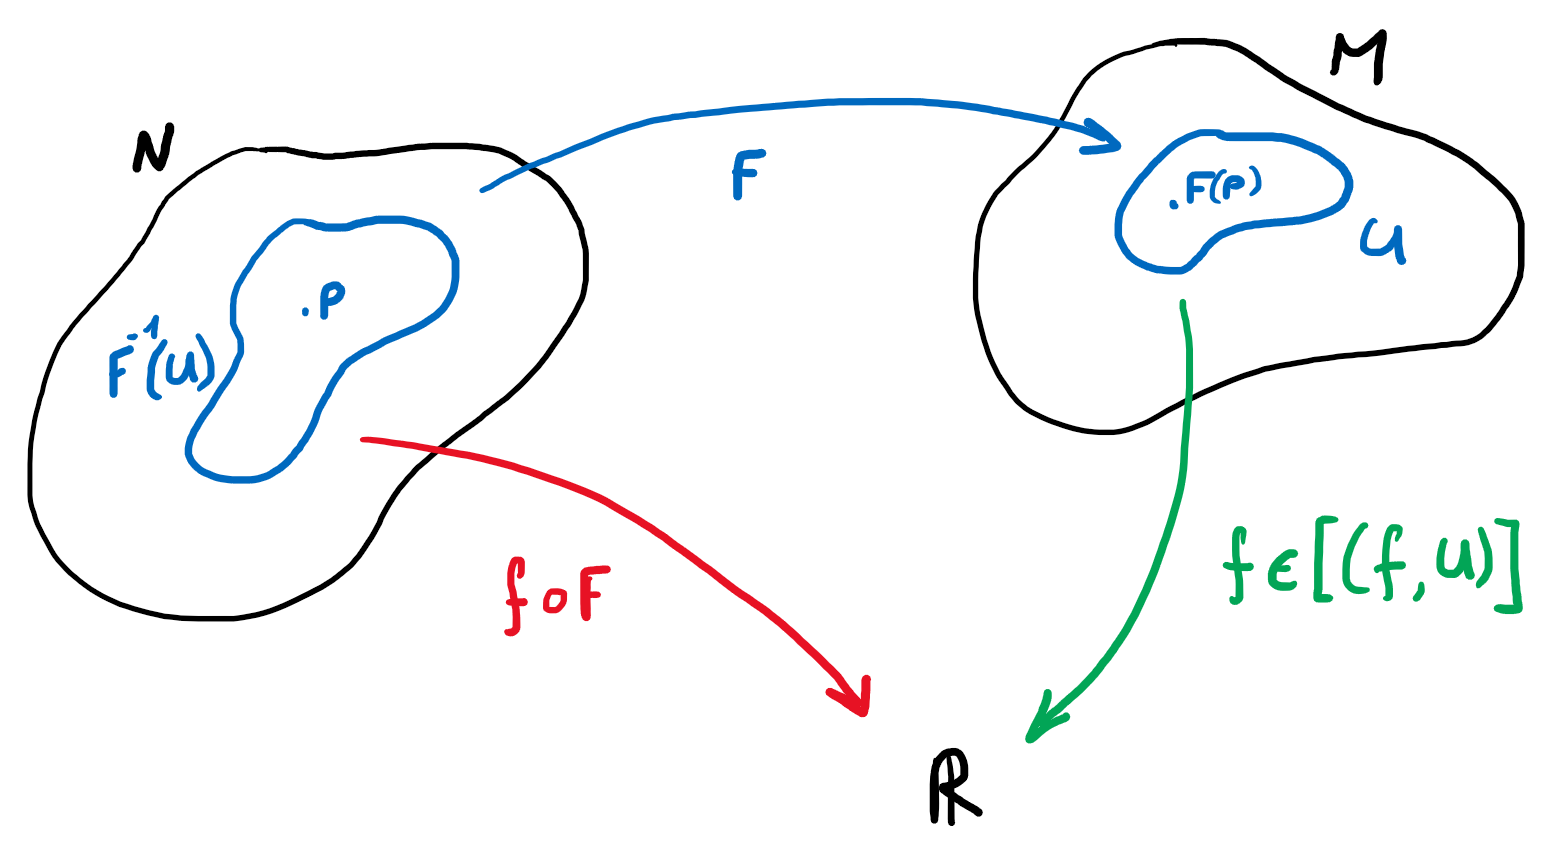
\includegraphics[width=0.5\textwidth,keepaspectratio]{img23}
\end{figure}

In breve

\begin{equation}
	F_{*p}(X_{p})(f) \doteq X_{p}(f \circ F) \in \R
\end{equation}

dove l'applicazione $ F_{*p}(X_{p}) : C_{F(p)}^{\infty}(M) \to \R $ rispetta la $ \R $-linearità

\begin{align}
	\begin{split}
		F_{*p}(X_{p})(\lambda f + \mu g) &= X_{p}((\lambda f + \mu g) \circ F)\\
		&= X_{p}(\lambda f \circ F + \mu g \circ F)\\
		&= \lambda X_{p}(f \circ F) + \mu X_{p}(g \circ F)\\
		&= \lambda F_{*p}(X_{p})(f) + \mu F_{*p}(X_{p})(g)
	\end{split}
\end{align}

in quanto $ X_{p} \in \der_{p}(C_{p}^{\infty}(N)) $ è $ \R $-lineare, e rispetta anche la regola di Leibniz

\begin{align}
	\begin{split}
		F_{*p}(X_{p})(f \cdot g) &= X_{p}((f \cdot g) \circ F)\\
		&= X_{p}((f \circ F) \cdot (g \circ F))\\
		&= X_{p}(f \circ F) \cdot (g \circ F)(p) + (f \circ F)(p) \cdot X_{p}(g \circ F)\\
		&= F_{*p}(X_{p})(f) \cdot g(F(p)) + f(F(p)) \cdot F_{*p}(X_{p})(g)
	\end{split}
\end{align}

in quanto $ X_{p}$ rispetta la regola di Leibniz, dunque $ F_{*p}(X_{p}) \in \der_{F(p)}(C_{F(p)}^{\infty}(M)) $.

\subsubsection{Proprietà del differenziale di un'applicazione}

\paragraph{1. Linearità}

Per mostrare che $ F_{*p} : T_{p}(N) \to T_{F(p)}(M) $ sia un'applicazione lineare, prendiamo due vettori $ X_{p},Y_{p} \in T_{p}(N) $, due numeri reali $ \alpha,\beta \in \R $ e una funzione $ f \in [(f,U)] \in C_{F(p)}^{\infty}(M) $

\begin{align}
	\begin{split}
		F_{*p}(\alpha X_{p} + \beta Y_{p})(f) &= (\alpha X_{p} + \beta Y_{p})(f \circ F)\\
		&= \alpha X_{p}(f \circ F) + \beta Y_{p}(f \circ F)\\
		&= \alpha F_{*p}(X_{p})(f) + \beta F_{*p}(Y_{p})(f)
	\end{split}
\end{align}

da cui

\begin{equation}
	F_{*p}(\alpha X_{p} + \beta Y_{p}) = \alpha F_{*p}(X_{p}) + \beta F_{*p}(Y_{p})
\end{equation}

\paragraph{2. Regola della catena}

Siano $ N $, $ M $ e $ P $ tre varietà differenziabili e $ F : N \to M $ e $ G : M \to P $ due applicazioni lisce, il differenziale della composizione delle due applicazioni in un punto $ p \in N $ vale

\begin{equation}
	(G \circ F)_{*p} = G_{*F(p)} \circ F_{*p}
\end{equation}

in quanto

\begin{align}
	\begin{split}
		F_{*p} : T_{p}(N) &\to T_{F(p)}(M)\\
		G_{*F(p)} : T_{F(p)}(M) &\to T_{G(F(p))}(P)
	\end{split}
\end{align}

La dimostrazione di questa relazione si ottiene applicando la composizione a $ X_{p} \in T_{p}(N) $ a sua volta applicato a $ f \in [(f,U)] \in C_{G(F(p))}^{\infty}(P) $

\begin{align}
	\begin{split}
		(G \circ F)_{*p} (X_{p})(f) &= X_{p} (f \circ G \circ F)\\
		&= F_{*p} (X_{p}) (f \circ G)\\
		&= G_{*F(p)} (F_{*p} (X_{p})(f))\\
		&= (G_{*F(p)} \circ F_{*p})(X_{p})(f)
	\end{split}
\end{align}

\paragraph{3. Proprietà funtoriali}

Il differenziale dell'identità $ \id_{N} : N \to N $ in punto $ p \in N $ è l'identità dello spazio tangente, i.e.
	
\begin{equation}
	(\id_{N})_{*p} = \id_{T_{p}(N)}
\end{equation}

in quanto

\begin{align}
	\begin{split}
		(\id_{N})_{*p} (X_{p})(f) &= X_{p} (f \circ \id_{N})\\
		&= X_{p}(f)
	\end{split}
\end{align}

Sia un diffeomorfismo $ F : N \to M $, allora $ F_{*p} : T_{p}(N) \to T_{F(p)}(M) $ è un isomorfismo tra spazi vettoriali: essendo $ F $ un diffeomorfismo, esiste una funzione $ G : M \to N $ per cui

\begin{equation}
	\begin{cases}
		G \circ F = \id_{N}\\
		F \circ G = \id_{M}
	\end{cases}
\end{equation}

dunque
	
\begin{align}
	\begin{split}
		(G \circ F)_{*p} &= G_{*F(p)} \circ F_{*p}\\
		&= (\id_{N})_{*p}\\
		&= \id_{T_{p}(N)}\\\\
		%
		(F \circ G)_{*F(p)} &= F_{*p} \circ G_{*F(p)}\\
		&= (\id_{M})_{*F(p)}\\
		&= \id_{T_{F(p)}(M)}
	\end{split}
\end{align}

perciò $ (F_{*p})^{-1} = G_{*F(p)} $ (inversa destra e sinistra).

\paragraph{4. Invarianza differenziabile della dimensione}

\begin{theorem}
	Sia $ F : U \to V $ un diffeomorfismo tra gli aperti $ U \subset \R^{n} $ e $ V \subset \R^{m} $, allora $ n = m $.
\end{theorem}

Conseguentemente, la definizione di varietà differenziabile è ben posta in quanto un diffeomorfismo non può legare un aperto ad un altro aperto di dimensione diversa dal primo.

\begin{proof}
	Essendo $ F : U \to V $ un diffeomorfismo, sappiamo che
	
	\begin{equation}
		F_{*p} : T_{p}(U) = T_{p}(\R^{n}) \to T_{F(p)}(V) = T_{F(p)}(\R^{m})
	\end{equation}

	è un isomorfismo, ma un isomorfismo tra due spazi di dimensione finita può esistere solo se i due spazi hanno la stessa dimensione, il che implica
	
	\begin{equation}
		\dim(T_{p}(\R^{n})) = \dim(T_{F(p)}(\R^{m})) \implies n = m
	\end{equation}
\end{proof}

Nel caso topologico non si può utilizzare questo procedimento in quanto ha senso calcolare il differenziale solo per funzioni che siano lisce, condizione non necessaria per le funzioni in topologia.

\paragraph{5. Base per $ T_{p}(N) $}

Sia $ N $ una varietà differenziabile, $ (U,\phi) \in N $ una sua carta con $ \phi = (x^{1},\dots,x^{n}) $ e $ p \in (U,\phi) $ un punto della varietà: l'insieme

\begin{equation}
	\mathcal{B}_{T_{p}(N)} = \left\{ \eval{ \pdv{x^{1}} }_{p}, \dots, \eval{ \pdv{x^{n}} }_{p} \right\}
\end{equation}

è una base per $ T_{p}(N) = \der_{p}(C_{p}^{\infty}(N)) $ in quanto

\begin{equation}
	\left. \dfrac{\partial}{\partial x^{i}} \right|_{p} \in T_{p}(N) \qcomma \forall i=1,\dots,n
\end{equation}

conseguentemente

\begin{equation}
	\dim(T_{p}(N)) = \dim(N)
\end{equation}

\begin{proof}
	Sappiamo che l'applicazione $ \phi : U \to \phi(U) \subset \R^{n} $ appartenente alla carta $ (U,\phi) $ non è solo un omeomorfismo ma anche un diffeomorfismo dunque il suo differenziale
	
	\begin{equation}
		\phi_{*p} : T_{p}(U) = T_{p}(N) \to T_{\phi(p)}(\phi(U)) = T_{\phi(p)}(\R^{n})
	\end{equation}

	è un isomorfismo tra spazi vettoriali.\\
	Calcoliamo ora l'azione di $ \phi_{*p} $ in un vettore generico della base $ \mathcal{B}_{T_{p}(N)} $:
	
	\begin{align}
		\begin{split}
			\phi_{*p} \left( \left. \dfrac{\partial}{\partial x^{i}} \right|_{p} \right) (f) &= \left. \dfrac{\partial}{\partial x^{i}} \right|_{p} (f \circ \phi)\\
			&= \left. \dfrac{\partial}{\partial r^{i}} \right|_{\phi(p)} (f \circ \phi \circ \phi^{-1})\\
			&= \left. \dfrac{\partial}{\partial r^{i}} \right|_{\phi(p)} f
		\end{split}
	\end{align}

	per $ \forall f \in [(f,U)] \in C_{\phi(p)}^{\infty}(N) $, perciò
	
	\begin{equation}
		\phi_{*p} \left( \left. \dfrac{\partial}{\partial x^{i}} \right|_{p} \right) = \left. \dfrac{\partial}{\partial r^{i}} \right|_{\phi(p)} \qcomma \forall i=1,\dots,n
	\end{equation}

	Essendo la derivata parziale in $ r^{i} $ un elemento di base e $ \phi_{*p} $ un isomorfismo che, in quanto tale, porta basi in basi, le derivate parziali in $ x^{i} $ sono quindi una base per $ T_{p}(N) $.
\end{proof}

\paragraph{6. Matrice dell'applicazione differenziale (aperti euclidei)}

Siano $ U = N \subset \R^{n} $ e $ V = M \subset \R^{m} $ aperti, sia $ F : U \to V $ un'applicazione liscia e sia $ p \in U $, il differenziale sarà

\begin{equation}
	F_{*p} : T_{p}(U) = T_{p}(\R^{n}) \to T_{F(p)}(V) = T_{F(p)}(\R^{m})
\end{equation}

Si possono identificare gli spazi tangenti in $ U $ e $ V $ con i rispettivi in $ \R^{n} $ e $ \R^{m} $ in quanto l'algebra considerata non dipende dall'aperto scelto intorno al punto, e.g. $ C_{p}^{\infty}(U) = C_{p}^{\infty}(\R^{n}) $.\\
Siano

\begin{equation}
	\mathcal{B}_{T_{p}(U)} = \left\{ \eval{ \pdv{r^{1}} }_{p}, \dots, \eval{ \pdv{r^{n}} }_{p} \right\}
\end{equation}

una base per $ T_{p}(U) $ e

\begin{equation}
	\mathcal{B}_{T_{F(p)}(V)} = \left\{ \eval{ \pdv{r^{1}} }_{F(p)}, \dots, \eval{ \pdv{r^{m}} }_{F(p)} \right\}
\end{equation}

una base per $ T_{F(p)}(V) $, allora gli elementi della matrice dell'applicazione $ F_{*p} $ sono dati da

\begin{equation}
	F_{*p} \left( \left. \dfrac{\partial}{\partial r^{j}} \right|_{p} \right) = \sum_{k=1}^{m} a_{kj} \left( \left. \dfrac{\partial}{\partial r^{k}} \right|_{F(p)} \right) \qcomma j=1,\dots,n
\end{equation}

in quanto $ F_{*p} $ è lineare. Le incognite sono le $ a_{kj} $ e, per trovarle, applichiamo entrambi i membri dell'equazione allo stesso oggetto, i.e. la proiezione naturale in $ \R^{m} $

\begin{align}
	\begin{split}
		r^{i} : \R^{m} &\to \R\\
		(x^{1},\dots,x^{m}) &\mapsto x^{i}
	\end{split}
\end{align}

dunque prendiamo il secondo membro

\begin{align}
	\begin{split}
		\sum_{k=1}^{m} a_{kj} \left( \left. \dfrac{\partial}{\partial r^{k}} \right|_{F(p)} r^{i} \right) &= \sum_{k=1}^{m} a_{kj} \left( \left. \dfrac{\partial r^{i}}{\partial r^{k}} \right|_{F(p)} \right)\\
		&= \sum_{k=1}^{m} a_{kj} \left( \dfrac{\partial r^{i}}{\partial r^{k}} \right)\\
		&= \sum_{k=1}^{m} a_{kj} \delta_{ik}\\
		&= a_{ij}
	\end{split}
\end{align}

dove $ [a_{ij}] \in M_{m,n}(\R) $ con $ i $ e $ j $ indici di riga e colonna rispettivamente. Siccome

\begin{align}
	\begin{split}
		F : U &\to V\\
		q &\mapsto (F^{1}(q),\dots,F^{m}(q))
	\end{split}
\end{align}

allora

\begin{align}
	\begin{split}
		r^{i} \circ F : U &\to V\\
		q &\mapsto F^{i}(q)
	\end{split}
\end{align}

a questo punto possiamo calcolare il primo membro applicato a $ r^{i} $

\begin{align}
	\begin{split}
		F_{*p} \left( \left. \dfrac{\partial}{\partial r^{j}} \right|_{p} \right) (r^{i}) &= \left. \dfrac{\partial}{\partial r^{j}} \right|_{p} (r^{i} \circ F)\\
		&= \left. \dfrac{\partial}{\partial r^{j}} \right|_{p} (r^{i} \circ F)\\
		&= \left. \dfrac{\partial}{\partial r^{j}} \right|_{p} F^{i}\\
		&= \dfrac{\partial F^{i}}{\partial r^{j}} (p)
	\end{split}
\end{align}

perciò

\begin{equation}
	a_{ij} = \dfrac{\partial F^{i}}{\partial r^{j}} (p)
\end{equation}

dunque le incognite corrispondono alle entrate della matrice jacobiana della funzione $ F $, i.e. $ [a_{ij}] = J(F)(p) $.\\
In generale, sia un'applicazione lineare

\begin{align}
	\begin{split}
		L : \R^{n} &\to \R^{m}\\
		v &\mapsto A v
	\end{split}
\end{align}

dove $ v = [r^{1},\dots,r^{n}]^{T} $ e $ A = [A_{ij}] \in M_{m,n}(\R) $, allora il suo jacobiano coincide proprio con la matrice della rappresentazione, i.e. $ J(L)(p) \equiv A $. Dato questo, possiamo scrivere che se un'applicazione è lineare allora $ L_{*p} \equiv L $.

\paragraph{7. Cambio di base}

Siano $ N $ una varietà differenziabile, un suo punto $ p \in N $ e due sue carte $ (U,\phi) $ e $ (U,\psi) $ con $ \phi = (x^{1},\dots,x^{n}) $ e $ \psi = (y^{1},\dots,y^{n}) $. Le basi per $ T_{p}(N) $ date da queste due funzioni sono legate da

\begin{equation}
	\left. \dfrac{\partial}{\partial x^{j}} \right|_{p} = \sum_{k=1}^{n} \dfrac{\partial y^{k}}{\partial x^{j}} (p) \left( \left. \dfrac{\partial}{\partial y^{k}} \right|_{p} \right)
\end{equation}

\begin{proof}
	La derivata in $ x^{j} $ appartiene allo spazio tangente $ T_{p}(N) $, dunque
	
	\begin{equation}
		\left. \dfrac{\partial}{\partial x^{j}} \right|_{p} = \sum_{k=1}^{n} a_{kj} \left( \left. \dfrac{\partial}{\partial y^{k}} \right|_{p} \right)
	\end{equation}

	Per trovare le $ a_{kj} $ applico entrambi i membri dell'equazione precedente alla funzione $ y^{i} : U \to \R $. Per il secondo membro
	
	\begin{align}
		\begin{split}
			\sum_{k=1}^{n} a_{kj} \left( \left. \dfrac{\partial}{\partial y^{k}} \right|_{p} y^{i} \right) &= \sum_{k=1}^{n} a_{kj} \left( \left. \dfrac{\partial y^{i}}{\partial y^{k}} \right|_{p} \right)\\
			&= \sum_{k=1}^{n} a_{kj} \left( \dfrac{\partial y^{i}}{\partial y^{k}}\right)\\
			&= \sum_{k=1}^{n} a_{kj} \delta_{ik}\\
			&= a_{ij}
		\end{split}
	\end{align}

	per il primo
	
	\begin{equation}
		\eval{ \pdv{x^{j}} }_{p} y^{j} = \pdv{y^{i}}{x^{j}} (p)
	\end{equation}

	perciò
	
	\begin{equation}
		a_{ij} = \pdv{y^{i}}{x^{j}} (p)
	\end{equation}
\end{proof}

\paragraph{8. Matrice dell'applicazione differenziale (varietà differenziabili)}

Siano $ F : N \to M $ un'applicazione liscia, un punto $ p \in N $ e due carte $ (U,\phi) \in N $ e $ (V,\psi) \in M $ con $ \phi = (x^{1},\dots,x^{n}) $ e $ \psi = (y^{1},\dots,y^{n}) $ e con $ F(U) \subset V $. Siano inoltre

\begin{align}
	\begin{split}
		\mathcal{B}_{T_{p}(N)} &= \left\{ \eval{ \pdv{x^{1}} }_{p}, \dots, \eval{ \pdv{x^{n}} }_{p} \right\}\\
		\mathcal{B}_{T_{F(p)}(M)} &= \left\{ \eval{ \pdv{y^{1}} }_{F(p)}, \dots, \eval{ \pdv{y^{m}} }_{F(p)} \right\}
	\end{split}
\end{align}

La matrice associata al differenziale $ F_{*p} : T_{p}(N) \to T_{F(p)}(M) $ rispetto alla base $ \mathcal{B}_{T_{p}(N)} $ è la matrice jacobiana

\begin{equation}
	J(F)(p) = \left[ \dfrac{\partial F^{i}}{\partial x^{j}} (p) \right]
\end{equation}

perciò

\begin{equation}
	F_{*p} \left( \left. \dfrac{\partial}{\partial x^{j}} \right|_{p} \right) = \sum_{k=1}^{n} \left( \dfrac{\partial F^{k}}{\partial x^{j}} (p) \right) \left( \left. \dfrac{\partial}{\partial y^{k}} \right|_{F(p)} \right)
\end{equation}

\begin{proof}
	In generale, essendo il differenziale una funzione lineare
	
	\begin{equation}
		F_{*p} \left( \left. \dfrac{\partial}{\partial x^{j}} \right|_{p} \right) = \sum_{k=1}^{n} a_{kj} \left( \left. \dfrac{\partial}{\partial y^{k}} \right|_{F(p)} \right)
	\end{equation}
	
	Se applichiamo il secondo membro a $ y^{i} $
	
	\begin{align}
		\begin{split}
			\sum_{k=1}^{n} a_{kj} \left( \left. \dfrac{\partial}{\partial y^{k}} \right|_{F(p)} y^{i} \right) &= \sum_{k=1}^{n} a_{kj} \left( \left. \dfrac{\partial y^{i}}{\partial y^{k}} \right|_{F(p)} \right)\\
			&= \sum_{k=1}^{n} a_{kj} \left( \dfrac{\partial y^{i}}{\partial y^{k}} \right)\\
			&= \sum_{k=1}^{n} a_{kj} \delta_{ik}\\
			&= a_{ij}
		\end{split}
	\end{align}
	
	e per il primo membro
	
	\begin{align}
		\begin{split}
			F_{*p} \left( \left. \dfrac{\partial}{\partial x^{j}} \right|_{p} \right) (y^{i}) &= \left. \dfrac{\partial}{\partial x^{j}} \right|_{p} (y^{i} \circ F)\\
			&= \left. \dfrac{\partial}{\partial x^{j}} \right|_{p} F^{i}\\
			&= \dfrac{\partial F^{i}}{\partial x^{j}} (p)
		\end{split}
	\end{align}
\end{proof}

\begin{remark}
	Possiamo enunciare il teorema della funzione inversa utilizzando il differenziale al posto dello jacobiano:
	
	\begin{theorem}
		Sia $ F : N \to M $ un'applicazione liscia dove $ \dim(N) = \dim(M) $ e sia un punto $ p \in N $, allora $ F $ è un diffeomorfismo locale in $ p $ se e solo se il suo differenziale $ F_{*p} $ è un isomorfismo.
	\end{theorem}

	Questo perché lo jacobiano è invertibile se e solo se il differenziale è un isomorfismo.
\end{remark}

\subsection{Categorie}

Una \textit{categoria} $ \mathfrak{C} $ consiste di una collezione\footnote{%
	Utilizzeremo il termine "collezione" al posto di "insieme" per evitare contraddizioni logiche, e.g. in situazioni dove potrebbe essere presente la locuzione "insiemi di insiemi".%
} di oggetti $ Ob(\mathfrak{C}) $ e per ogni coppia di elementi appartenenti alla categoria $ A,B \in Ob(\mathfrak{C}) $ esiste un insieme non vuoto $ Mor(A,B) $ dei morfismi\footnote{%
	Un morfismo è una mappa tra due oggetti che conserva la struttura dell'oggetto sorgente nell'oggetto obbiettivo; ad esempio, è la generalizzazione nella teoria delle categorie delle funzioni nella teoria degli insiemi o delle funzioni continue in topologia.%
} da $ A $ a $ B $ tale che siano soddisfatte le seguenti condizioni:

\begin{equation}
	\begin{cases}
		\E g \circ f \in Mor(A,C)\footnotemark, & \forall f \in Mor(A,B), \, \forall g \in Mor(B,C)\\
		\E \mathbbm{1}_{A} \in Mor(A,A) \, \mid \, f \circ \mathbbm{1}_{A} = f, & \forall f \in Mor(A,B)\\
		\E \mathbbm{1}_{B} \in Mor(B,B) \, \mid \, \mathbbm{1}_{A} \circ g = g, & \forall g \in Mor(B,A)\\
		(f \circ g) \circ h = f \circ (g \circ h), & \forall f \in Mor(A,B), \forall g \in Mor(B,C), \forall h \in Mor(C,D)
	\end{cases}
\footnotetext{Il simbolo $ \circ $ indica la composizione ma, nella teoria delle categorie, non è necessariamente la composizione come si intende per le funzioni in teoria degli insiemi; nonostante ciò, vedremo solo esempi in cui le due composizioni sopraccitate coincidono.}
\end{equation}

\subsubsection{\textit{Esempi}}

\paragraph{0. Insiemi}

Sia $ \mathfrak{C} $ è la categoria degli insiemi, allora

\begin{equation}
	Ob(\mathfrak{C}) = \{ \text{collezione di tutti gli insiemi} \}
\end{equation}

dove l'insieme dei morfismi è dato da

\begin{equation}
	Mor(A,B) = \{ \text{applicazioni } f : A \to B \}
\end{equation}

per $ \forall A,B \in Ob(\mathfrak{C}) $.\\
Tutte le proprietà delle categorie sono soddisfatte e la composizione $ \circ $ corrisponde a quella usuale.

\paragraph{1. Spazi vettoriali su $ \R $}

Sia $ \mathfrak{C} $ la categoria degli spazi vettoriali su $ \R $, allora

\begin{equation}
	Ob(\mathfrak{C}) = \{ \text{collezione di tutti gli spazi vettoriali su } \R \}
\end{equation}

dove l'insieme dei morfismi è dato da

\begin{equation}
	Mor(V,W) = Hom(V,W) = \{ \text{applicazioni } \R \text{ lineari } f : V \to W \}
\end{equation}

per $ \forall V,W \in Ob(\mathfrak{C}) $.\\
Tutte le proprietà delle categorie sono soddisfatte e la composizione $ \circ $ corrisponde a quella usuale.

\paragraph{2. Spazi topologici}

Sia $ \mathfrak{Top} $ la categoria degli spazi topologici, allora

\begin{equation}
	Ob(\mathfrak{Top}) = \{ \text{collezione di tutti gli spazi topologici} \}
\end{equation}

dove l'insieme dei morfismi è dato da

\begin{equation}
	Mor(X,Y) = C^{0}(X,Y) = \{ \text{applicazioni continue } f : X \to Y \}
\end{equation}

per $ \forall X,Y \in Ob(\mathfrak{Top}) $.\\
Tutte le proprietà delle categorie sono soddisfatte e la composizione $ \circ $ corrisponde a quella usuale.

\paragraph{3. Varietà differenziabili}

Sia $ \mathfrak{C} $ la categoria delle varietà differenziabili, allora

\begin{equation}
	Ob(\mathfrak{C}) = \{ \text{collezione di tutte le varietà differenziabili} \}
\end{equation}

dove l'insieme dei morfismi è dato da

\begin{equation}
	Mor(N,M) = \{ \text{applicazioni lisce } F : N \to M \}
\end{equation}

per $ \forall N,M \in Ob(\mathfrak{C}) $.\\
Tutte le proprietà delle categorie sono soddisfatte e la composizione $ \circ $ corrisponde a quella usuale.

\paragraph{4. Varietà differenziabili puntate}

Sia $ \mathfrak{C} $ la categoria delle varietà differenziabili puntate, i.e. varietà in cui è fissato un punto\footnote{%
	Due varietà differenziali puntate sono diverse anche se si cambia solo il punto fissato, e.g. $ (M,p) \neq (M,q) \mid p \neq q $}, allora

\begin{equation}
	Ob(\mathfrak{C}) = \{ \text{collezione di tutte le coppie } (M,p) \, \mid M \text{ varietà differenziabili}, \, p \in M \}
\end{equation}

dove l'insieme dei morfismi è dato da

\begin{equation}
	Mor((M,p),(N,q)) = \{ \text{applicazioni lisce } F : N \to M \, \mid \, F(p)=q \}
\end{equation}

per $ \forall (M,p),(N,q) \in Ob(\mathfrak{C}) $.\\
Tutte le proprietà delle categorie sono soddisfatte e la composizione $ \circ $ corrisponde a quella usuale.

\subsubsection{Isomorfismi}

Data una categoria $ \mathfrak{C} $, la definizione di oggetti isomorfi è la seguente:

\begin{equation}
	A \simeq B \text{ isomorfi} \iff \E f \in Mor(A,B) \wedge g \in Mor(B,A) \, \mid \, g \circ f = \mathbbm{1}_{A} \wedge f \circ g = \mathbbm{1}_{B}
\end{equation}

dove $ A,B \in Ob(\mathfrak{C}) $, $ \mathbbm{1}_{A} \in Mor(A,A) $ e $ \mathbbm{1}_{B} \in Mor(B,B) $.\\
Per esempio, per la categoria degli insiemi, due oggetti sono isomorfi se esistono due applicazioni l'una inversa dell'altra tali che associno questi due oggetti; dunque, .

\subsubsection{\textit{Esempi}}

\paragraph{0. Insiemi}

Due oggetti nella categoria degli insiemi sono isomorfi se hanno la stessa cardinalità, i.e. $ A \simeq B \iff \# A = \# B $, perciò esiste una bigezione tra i due oggetti.

\paragraph{1. Spazi vettoriali su $ \R $}

Due oggetti nella categoria degli spazi vettoriali sono isomorfi quando lo sono come spazi vettoriali, i.e.

\begin{equation}
	V \simeq W \iff V \stackrel{sp.vett.}{\simeq} W
\end{equation}

\paragraph{2. Spazi topologici}

Due oggetti nella categoria degli spazi topologico sono isomorfi quando sono omeomorfi, i.e.

\begin{equation}
	X \simeq Y \iff V \stackrel{hom.}{\simeq} W
\end{equation}

\paragraph{3. Varietà differenziabili}

Due oggetti nella categoria delle varietà differenziabili sono isomorfi quando sono diffeomorfi, i.e.

\begin{equation}
	N \simeq M \iff N \stackrel{diff.}{\simeq} M
\end{equation}

\paragraph{4. Varietà differenziabili puntate}

Due oggetti nella categoria delle varietà differenziabili puntate sono isomorfi quando sono diffeomorfi, i.e.

\begin{equation}
	(N,p) \simeq (M,q) \iff \E F : N \to M \text{ diffeomorfismo} \, \mid \, N \stackrel{diff.}{\simeq} M \wedge F(p)=q
\end{equation}

\subsection{Funtori}

I \textit{funtori} i dividono in funtori \textit{covarianti} e \textit{controvarianti}.\\
Siano $ \mathfrak{C} $ e $ \mathfrak{D} $ due categorie, un \textit{funtore covariante} è una coppia di applicazioni identificate da $ \mathcal{F} $ tali che

\begin{equation}
	\begin{cases}
		\mathcal{F}(A) \in Ob(\mathfrak{D}), & \forall A \in Ob(\mathfrak{C})\\
		\mathcal{F}(f) \in Mor(\mathcal{F}(A),\mathcal{F}(B)), & \forall f \in Mor(A,B)
	\end{cases}
\end{equation}

rispettando l'identità e la composizione, i.e.

\begin{equation}
	\begin{cases}
		\mathcal{F}(\mathbbm{1}_{A}) = \mathbbm{1}_{\mathcal{F}(A)} \in Ob(\mathfrak{D}), & \forall \mathbbm{1}_{A} \in Mor(A,A)\\
		\mathcal{F}(g \circ f) = \mathcal{F}(g) \circ \mathcal{F}(f) & \forall f \in Mor(A,B), \forall g \in Mor(B,C)
	\end{cases}
\end{equation}

Il funtore differenziale covariante, date $ \mathfrak{C} $ la categoria delle varietà puntate e $ \mathfrak{D} $ la categoria degli spazi vettoriali, associa

\begin{equation}
	\begin{cases}
		\mathcal{F}((N,p)) = T_{p}(N), & \forall (N,p) \in Ob(\mathfrak{C}), \, T_{p}(N) \in Ob(\mathfrak{D})\\
		\mathcal{F}(F) = F_{*p} & \forall F \in Mor((N,p),(M,q)), \, F_{*p} \in Mor(T_{p}(N),T_{q=F(p)}(M))
	\end{cases}
\end{equation}

Per dimostrare che sia un funtore covariante, verifichiamo che rispetti l'identità

\begin{align}
	\begin{split}
		\mathcal{F}(\mathbbm{1}_{N}) &= (\mathbbm{1}_{N})_{*p}\\
		&= \mathbbm{1}_{T_{p}(N)}\\
		&= \mathbbm{1}_{\mathcal{F}((N,p))}
	\end{split}
\end{align}

e la composizione

\begin{align}
	\begin{split}
		\mathcal{F}(G \circ F) &= (G \circ F)_{*p}\\
		&= G_{*F(p)} \circ F_{*p}\\
		&= \mathcal{F}(G) \circ \mathcal{F}(F)
	\end{split}
\end{align}

per qualsiasi applicazione liscia tra varietà $ F : (N,p) \to (M,F(p)) $ e $ G : (M,F(p)) \to (P,G(F(p))) $ e qualsiasi varietà $ N $, $ M $ e $ P $ con $ p \in N $.\\\\
%
Siano $ \mathfrak{C} $ e $ \mathfrak{D} $ due categorie, un \textit{funtore controvariante} è una coppia di applicazioni identificate da $ \mathcal{F} $ tali che

\begin{equation}
	\begin{cases}
		\mathcal{F}(A) \in Ob(\mathfrak{D}), & \forall A \in Ob(\mathfrak{C})\\
		\mathcal{F}(f) \in Mor(\mathcal{F}(B),\mathcal{F}(A)), & \forall f \in Mor(A,B)
	\end{cases}
\end{equation}

rispettando l'identità e la composizione, i.e.

\begin{equation}
	\begin{cases}
		\mathcal{F}(\mathbbm{1}_{A}) = \mathbbm{1}_{\mathcal{F}(A)} \in Ob(\mathfrak{D}), & \forall \mathbbm{1}_{A} \in Mor(A,A)\\
		\mathcal{F}(g \circ f) = \mathcal{F}(f) \circ \mathcal{F}(g) & \forall f \in Mor(A,B), \forall g \in Mor(B,C)
	\end{cases}
\end{equation}

\begin{remark}
	Sia $ \mathcal{F} : \mathfrak{C} \to \mathfrak{D} $ un funtore (covariante o controvariante), allora
	
	\begin{equation}
		A \simeq B \implies \mathcal{F}(A) \simeq \mathcal{F}(B)
	\end{equation}
	
	per $ \forall A,B \in \mathfrak{C} $.
\end{remark}

\begin{proof}
	Per funtori covarianti, la definizione di isomorfismo asserisce che
	
	\begin{equation}
		A \simeq B \implies \E f \in Mor(A,B), g \in Mor(B,A) \, \mid \, g \circ f = \mathbbm{1}_{A} \wedge f \circ g = \mathbbm{1}_{B}
	\end{equation}
	
	Applicando il funtore a entrambi i membri
	
	\begin{align}
		\begin{split}
			\mathcal{F}(g \circ f) = \mathcal{F}(\mathbbm{1}_{A}) &\wedge \mathcal{F}(f \circ g) = \mathcal{F}(\mathbbm{1}_{B})\\
			\mathcal{F}(g) \circ \mathcal{F}(f) = \mathbbm{1}_{\mathcal{F}(A)} &\wedge \mathcal{F}(f) \circ \mathcal{F}(g) = \mathbbm{1}_{\mathcal{F}(B)}
		\end{split}
	\end{align}
	
	il quale dimostra che $ \mathcal{F}(A) \simeq \mathcal{F}(B) $.\\
	La dimostrazione per funtori controvarianti è analoga.
\end{proof}

\subsubsection{\textit{Esempi}}

\paragraph{1. Spazio duale}

Sia $ \mathfrak{C} $ la categoria degli spazi vettoriali su $ \R $, consideriamo il funtore controvariante $ \mathcal{F} : \mathfrak{C} \to \mathfrak{C} $ tale che

\begin{equation}
	\begin{cases}
		\mathcal{F}(V) = V^{*}, & \forall V \in Ob(\mathfrak{C})\\
		\mathcal{F}(f) = f^{*}, & \forall f \in Hom(V,W) = Mor(V,W)
	\end{cases}
\end{equation}

dove $ V^{*} $ è lo spazio duale\footnote{%
	Lo spazio duale $ V^{*} $ corrisponde all'insieme degli omeomorfismi da $ V $ a $ \R $, i.e. $ V^{*} = Hom(V,\R) $.%
} di $ V $ i cui oggetti sono applicazioni da $ V $ in $ \R $ e

\begin{align}
	\begin{split}
		f^{*} : W^{*} = Hom(W,\R) &\to V^{*} = Hom(\mathcal{F}(W),\mathcal{F}(V)) = Hom(W^{*},V^{*})\\
		\alpha &\mapsto f^{*}(\alpha) = \alpha \circ f
	\end{split}
\end{align}

Per dimostrare che sia un funtore controvariante, verifichiamo che rispetti l'identità

\begin{align}
	\begin{split}
		\mathcal{F}(\mathbbm{1}_{V}) &= \mathbbm{1}_{V}^{*}\\
		&= \mathbbm{1}_{V^{*}}\\
		&= \mathbbm{1}_{\mathcal{F}(V)}
	\end{split}
\end{align}

in quanto $ \mathbbm{1}_{V} : V \to V $ e $ \mathbbm{1}_{V}^{*} : V^{*} \to V^{*} $, e la composizione

\begin{align}
	\begin{split}
		\mathcal{F}(g \circ f) &= (g \circ f)^{*}\\
		&= f^{*} \circ g^{*}\\
		&= \mathcal{F}(f) \circ \mathcal{F}(g)
	\end{split}
\end{align}

per qualsiasi $ f \in Mor(V,W) $ e $ g \in Mor(W,Z) $, in quanto

\begin{align}
	\begin{split}
		(g \circ f)^{*}(\alpha) &= \alpha \circ g \circ f\\
		&= f^{*} (\alpha \circ g)\\
		&= f^{*} \circ g^{*} \circ \alpha
	\end{split}
\end{align}

\paragraph{2. Varietà puntate e isomorfismi}

Siano $ \mathfrak{C} $ la categoria delle varietà puntate e $ \mathfrak{D} $ la categoria degli spazi vettoriali. Il funtore differenziale covariante associa

\begin{equation}
	\begin{cases}
		\mathcal{F}((N,p)) = T_{p}(N), & \forall (N,p) \in Ob(\mathfrak{C}), \, T_{p}(N) \in Ob(\mathfrak{D})\\
		\mathcal{F}(F) = F_{*p} & \forall F \in Mor((N,p),(M,q)), \, F_{*p} \in Mor(T_{p}(N),T_{q=F(p)}(M))
	\end{cases}
\end{equation}

A questo punto, se due varietà puntate sono diffeomorfe $ (N,p) \simeq (M,q) $ allora i loro due spazi tangenti saranno isomorfi $ T_{q}(M) $.

\subsection{Curve su una varietà differenziabile}

Una \textit{curva} liscia $ c $ su una varietà differenziabile $ N $ è un'applicazione liscia tale che $ c : (a,b) \subset \R \to N $. Se $ 0 \in (a,b) $ diremo che $ c $ \textit{inizia} in $ c(0)=p $.

\begin{figure}[H]
	\centering
	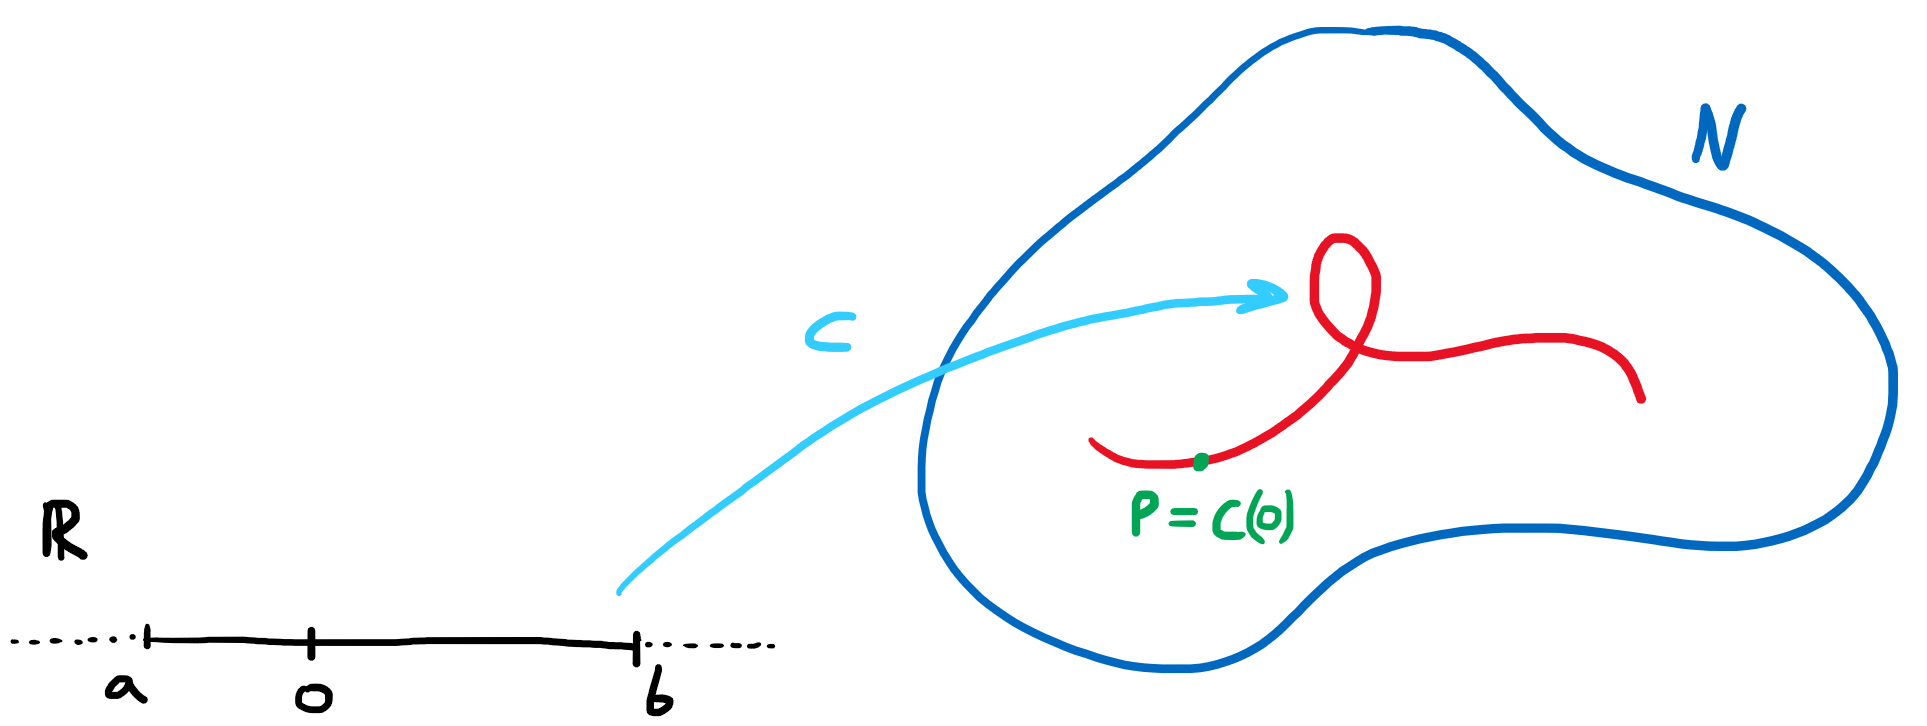
\includegraphics[width=0.5\textwidth,keepaspectratio]{img24}
\end{figure}

Definiamo il \textit{vettore tangente} o \textit{vettore velocità} $ c'(t_{0}) \in T_{c(t_{0})}(N) $ della curva $ c $, dove $ t_{0} \in (a,b) $, come

\begin{equation}
	c'(t_{0}) \doteq c_{*t_{0}} \left( \left. \dfrac{\operatorname{d}}{\operatorname{dt}} \right|_{t_{0}} \right)
\end{equation}

dove $ c_{*t} : T_{t_{0}}((a,b)) = T_{t_{0}}(\R) \to T_{c(t_{0})}(N) $.\\
Il vettore tangente $ c'(t_{0}) $ è dunque l'immagine, tramite l'applicazione lineare del differenziale $ c_{*t} $, del vettore $ (\sfrac{\operatorname{d}}{\operatorname{dt}}) |_{t_{0}} $, il quale rappresenta la base canonica\footnote{%
	La notazione che indica che un elemento di una base genera uno spazio è la seguente
	
	\begin{equation}
		\left\langle \left. \dfrac{\operatorname{d}}{\operatorname{dt}} \right|_{t_{0}} \right\rangle = T_{t_{0}}(\R)
	\end{equation}%
} di $ T_{t_{0}}(\R) $.

\begin{remark}
	Sia $ c : (a,b) \to \R $ una curva. Possiamo considerare sia la derivata di $ c $ nel punto $ t_{0} \in (a,b) $ sia il vettore tangente alla curva e le notazioni saranno le seguenti
	
	\begin{equation}
		\begin{cases}
			\dot{c}(t_{0}) \doteq \left. \dfrac{\operatorname{d}}{\operatorname{dt}} \right|_{t_{0}} c(t) \in \R & \text{derivata}\\\\
			%
			c'(t_{0}) \in T_{c(t_{0})}(\R) & \text{vettore tangente}
		\end{cases}
	\end{equation}
\end{remark}

Siccome $ c'(t_{0}) \in T_{c(t_{0})}(\R) $, possiamo scrivere il vettore tangente come

\begin{equation}
	c'(t_{0}) = a \, \left. \dfrac{\operatorname{d}}{\operatorname{dr}} \right|_{c(t_{0})}
\end{equation}

dove $ a \in \R $ e $ \langle \sfrac{\operatorname{d}}{\operatorname{dr}} |_{c(t_{0})} \rangle = T_{c(t_{0})}(\R) $.\\
Per determinare $ a $, applichiamo entrambi i membri dell'equazione alla funzione identità

\begin{align}
	\begin{split}
		r : \R &\to \R\\
		x &\mapsto x
	\end{split}
\end{align}

Per il secondo membro

\begin{align}
	\begin{split}
		\left( a \, \left. \dfrac{\operatorname{d}}{\operatorname{dr}} \right|_{c(t_{0})} \right) r &= a \, \left. \dfrac{\operatorname{dr}}{\operatorname{dr}} \right|_{c(t_{0})}\\
		&= a \, \dfrac{\operatorname{dr}}{\operatorname{dr}}\\
		&= a
	\end{split}
\end{align}

e per il primo membro

\begin{align}
	\begin{split}
		c'(t_{0})(r) &= c_{*t_{0}} \left( \left. \dfrac{\operatorname{d}}{\operatorname{dt}} \right|_{t_{0}} \right)(r)\\
		&= \left. \dfrac{\operatorname{d}}{\operatorname{dt}} \right|_{t_{0}} (r \circ c)\\
		&= \left. \dfrac{\operatorname{d}}{\operatorname{dt}} \right|_{t_{0}} c\\
		&= \dot{c}(t_{0})
	\end{split}
\end{align}

perciò

\begin{equation}
	c'(t_{0}) = \dot{c}(t_{0}) \left. \dfrac{\operatorname{d}}{\operatorname{dr}} \right|_{c(t_{0})}
\end{equation}

nel caso in cui il codominio sia $ \R $.

\begin{definition}[Espressione locale del vettore tangente a una curva liscia]\label{loc-exp-tan-cur}
	Siano $ c : (a,b) \to N $ una curva liscia e $ (U,\phi) \in N $ una carta con $ \phi = (x^{1},\dots,x^{n}) $ tale che $ c((a,b)) \in U $.
	
	\begin{figure}[H]
		\centering
		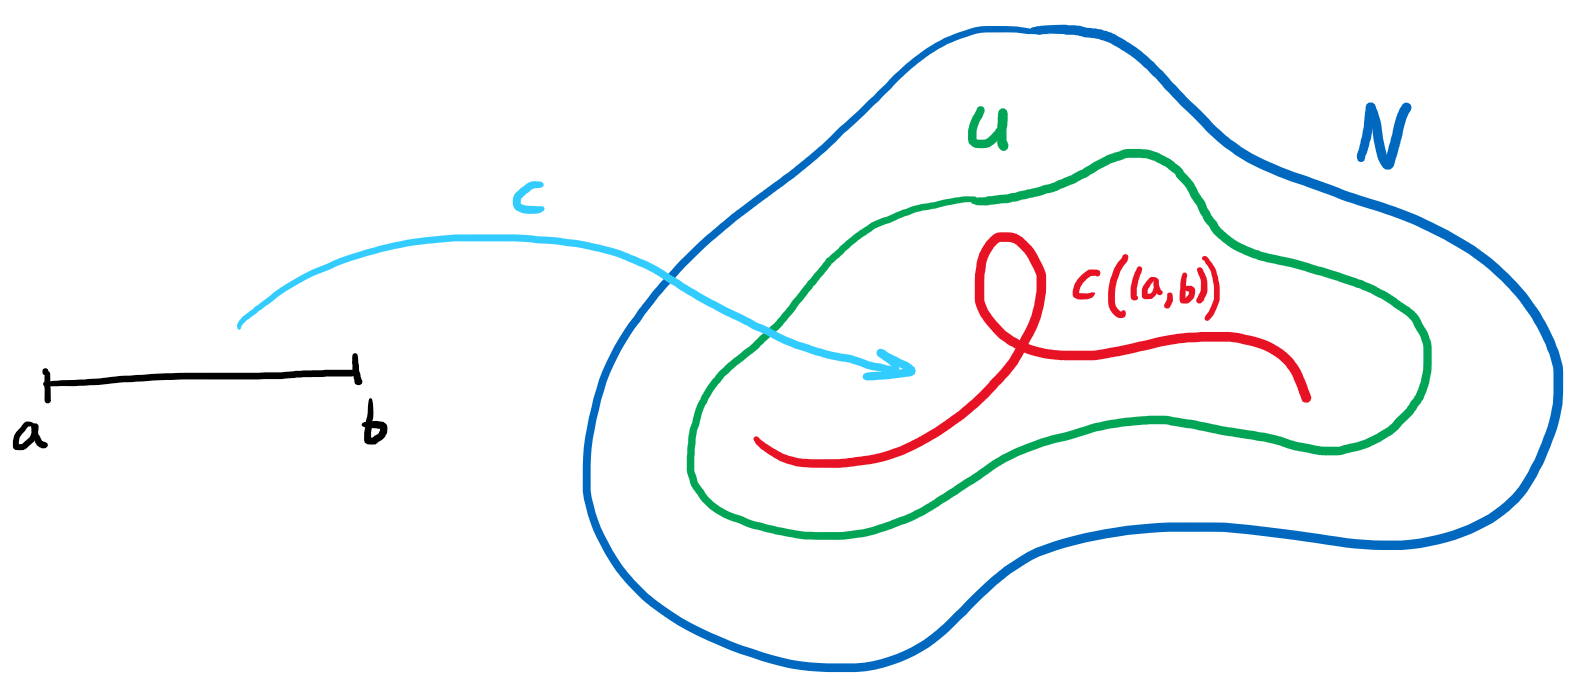
\includegraphics[width=0.5\textwidth,keepaspectratio]{img25}
	\end{figure}
	
	Siano $ c^{i} : (a,b) \to \R $ le componenti di $ c $ rispetto alla carta fissata, cioè $ c^{i} = x^{i} \circ c $ per $ \forall i=1,\dots,n $. Il vettore tangente alla curva si scrive come
	
	\begin{equation}
		c'(t_{0}) = \sum_{i=1}^{n} \dot{c}_{i}(t_{0}) \left. \dfrac{\partial}{\partial x^{i}} \right|_{c(t_{0})}
	\end{equation}

	In particolare, se $ N = \R^{n} $ allora
	
	\begin{equation}
		c'(t_{0}) = \sum_{i=1}^{n} \dot{c}_{i}(t_{0}) \left. \dfrac{\partial}{\partial r^{i}} \right|_{c(t_{0})}
	\end{equation}

	dove $ \dot{c}_{i}(t_{0}) $ può essere identificato con il vettore colonna $ [\dot{c}_{1}(t_{0}),\dots,\dot{c}_{n}(t_{0})]^{T} $.
\end{definition}

Un esempio potrebbe essere la curva

\begin{align}
	\begin{split}
		c : \R &\to \R^{2}\\
		t &\mapsto (t,t^{3})
	\end{split}
\end{align}

da cui $ c'(t_{0}) = (1, 3 t_{0}^{2}) $, nella quale espressione si identifica il vettore tangente con il vettore di $ \R^{2} $ al secondo membro.

\begin{proof}
	Per definizione $ c'(t_{0}) \in T_{c(t_{0})}(N) $ dunque
	
	\begin{equation}
		c'(t_{0}) = \sum_{i=1}^{n} a^{i} \left. \dfrac{\partial}{\partial x^{i}} \right|_{c(t_{0})}
	\end{equation}

	con $ a^{i} \in \R $ per $ i=1,\dots,n $, in quanto $ \langle \sfrac{\partial}{\partial x^{i}} |_{c(t_{0})} \rangle = T_{c(t_{0})}(N) $.\\
	Valutiamo ora entrambi i membri applicati alla funzione coordinata
	
	\begin{align}
		\begin{split}
			x^{j} : U &\to \R\\
			(x^{1},\dots,x^{n}) &\mapsto x^{j}
		\end{split}
	\end{align}

	Per il secondo membro
	
	\begin{align}
		\begin{split}
			\left( \sum_{i=1}^{n} a_{i} \left. \dfrac{\partial}{\partial x^{i}} \right|_{c(t_{0})} \right) (x^{j}) &= \sum_{i=1}^{n} a^{i} \left. \dfrac{\partial x^{j}}{\partial x^{i}} \right|_{c(t_{0})}\\
			&= \sum_{i=1}^{n} a^{i} \dfrac{\partial x^{j}}{\partial x^{i}}\\
			&= \sum_{i=1}^{n} a^{i} \delta_{ij}\\
			&= a^{j}
		\end{split}
	\end{align}

	e per il primo
	
	\begin{align}
		\begin{split}
			c'(t_{0})(x^{j}) &= c_{*t_{0}} \left( \left. \dfrac{\operatorname{d}}{\operatorname{dt}} \right|_{t_{0}} \right)(x^{j})\\
			&= \left. \dfrac{\operatorname{d}}{\operatorname{dt}} \right|_{t_{0}} (x^{j} \circ c)\\
			&= \left. \dfrac{\operatorname{d}}{\operatorname{dt}} \right|_{t_{0}} c^{j}\\
			&= \dot{c}_{j}(t_{0})
		\end{split}
	\end{align}
\end{proof}

\subsubsection{Spazio tangente e curve}

Sia una curva liscia $ c : (a,b) \to N $ che inizi in $ c(0) = p \in N $, allora $ c'(t_{0}) \in T_{p}(N) $. Ogni vettore in $ T_{p}(N) $ è il vettore velocità di una curva liscia in $ N $ che inizia in $ p $.

\begin{definition}
	Siano $ N $ una varietà differenziabile, un suo punto $ p \in N $ e un vettore $ X_{p} \in T_{p}(N) $, allora
	
	\begin{equation}
		\E c : (-\varepsilon,\varepsilon) \ni 0 \to N \text{ curva liscia}, c(0) = p \, \mid \, c'(0) = X_{p}
	\end{equation}

	Questo mostra che
	
	\begin{equation}
		T_{p}(N) = \{ c'(0) \, \mid \, c : (-\varepsilon,\varepsilon) \ni 0 \to N \text{ curva liscia}, c(0) = p \}
	\end{equation}

	Questo insieme è più intuitivo, nonostante equivalente, dell'insieme delle derivazioni puntali dell'algebra dei germi delle funzioni lisce in un punto $ p $, i.e. $ T_{p}(N) = \der_{p}(C_{p}^{\infty}(N)) $.
\end{definition}

\begin{proof}
	Consideriamo il seguente schema
	
	\begin{figure}[H]
		\centering
		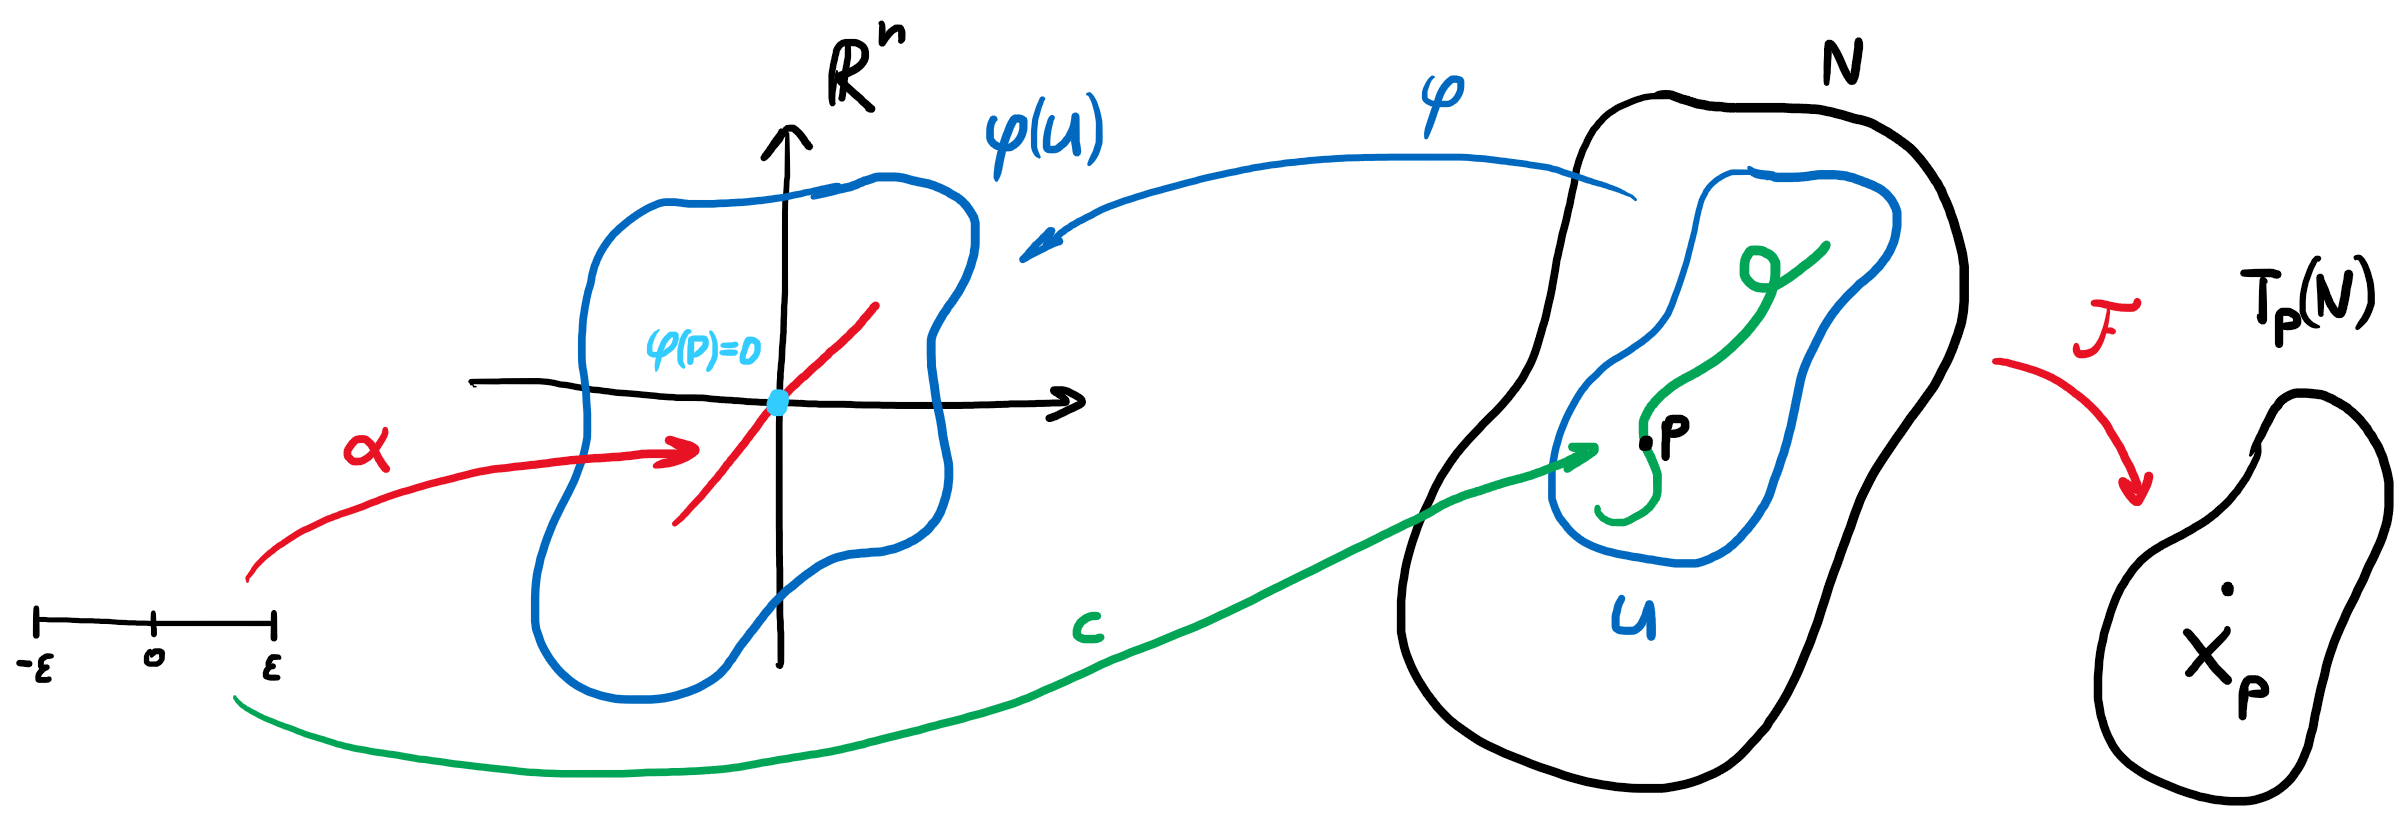
\includegraphics[width=0.7\textwidth,keepaspectratio]{img26}
	\end{figure}

	Fissiamo una carta $ (U,\phi) \in N $ con $ \phi = (x^{1},\dots,x^{n}) $ e $ p \in U $ la quale fisserà a sua volta una base per lo spazio tangente $ \langle \sfrac{\partial}{\partial x^{i}} |_{p} \rangle = T_{p}(N) $, perciò possiamo scrivere
	
	\begin{equation}
		X_{p} = \sum_{i=1}^{n} a^{i} \left. \dfrac{\partial}{\partial x^{i}} \right|_{p}
	\end{equation}

	con $ i=1,\dots,n $, in quanto abbiamo dimostrato che
	
	\begin{equation}
		\phi_{*p} \left( \left. \dfrac{\partial}{\partial x^{i}} \right|_{p} \right) = \left. \dfrac{\partial}{\partial r^{i}} \right|_{\phi(p)}
	\end{equation}
	
	Prendiamo ora l'applicazione
	
	\begin{align}
		\begin{split}
			\alpha : (-\varepsilon,\varepsilon) \ni 0 &\to \R^{n}\\
			t &\mapsto (a^{1} t, \dots, a^{n} t)
		\end{split}
	\end{align}

	la quale associa all'intervallo sorgente una retta: considerando $ \varepsilon $ opportuno, possiamo far in modo che $ \alpha((-\varepsilon,\varepsilon)) \subset \phi(U) $.\\
	La curva $ c : (-\varepsilon,\varepsilon) \ni 0 \to N $ corrisponderà dunque a $ c(t) = (\phi^{-1} \circ \alpha)(t) $ la quale è liscia in quanto composizione di funzioni lisce.\\
	Il vettore tangente alla curva in 0 è uguale a
	
	\begin{align}
		\begin{split}
			c'(0) &= c_{*0} \left( \left. \dfrac{\operatorname{d}}{\operatorname{dt}} \right|_{0} \right)\\
			&= (\phi^{-1} \circ \alpha)_{*0} \left( \left. \dfrac{\operatorname{d}}{\operatorname{dt}} \right|_{0} \right)\\
			&= (\phi^{-1}_{*\alpha(0)} \circ \alpha_{*0}) \left( \left. \dfrac{\operatorname{d}}{\operatorname{dt}} \right|_{0} \right)\\
			&= (\phi^{-1}_{*0} \circ \alpha_{*0}) \left( \left. \dfrac{\operatorname{d}}{\operatorname{dt}} \right|_{0} \right)\\
			&= \phi^{-1}_{*0} \left( \alpha_{*0} \left( \left. \dfrac{\operatorname{d}}{\operatorname{dt}} \right|_{0} \right) \right)\\
			&= \phi^{-1}_{*0} \left( \sum_{i=1}^{n} a^{i} \left. \dfrac{\partial}{\partial r^{i}} \right|_{0} \right)\\
			&= \sum_{i=1}^{n} a^{i} \phi^{-1}_{*0} \left( \left. \dfrac{\partial}{\partial r^{i}} \right|_{0} \right)\\
			&= \sum_{i=1}^{n} a^{i} \left. \dfrac{\partial}{\partial x^{i}} \right|_{0}\\
			&= X_{p}
		\end{split}
	\end{align}

	dove $ \alpha_{*0} $ con $ 0 \in \R $ mentre $ \phi^{-1}_{*0} $ con $ 0 \in \R^{n} $, inoltre
	
	\begin{equation}
		\alpha_{*0} \left( \left. \dfrac{\operatorname{d}}{\operatorname{dt}} \right|_{0} \right) = \sum_{i=1}^{n} a^{i} \left. \dfrac{\partial}{\partial r^{i}} \right|_{0}
	\end{equation}

	per la Proposizione \ref{loc-exp-tan-cur} in quanto $ \alpha $ è anch'essa una curva liscia e possiamo portare $ \phi_{*0} $ dentro la sommatoria in quanto applicazione lineare.
\end{proof}

\subsection{Differenziale tramite curve}

Siano $ X_{p} \in T_{p}(N) $ e $ f \in C^{\infty}(N) $, la notazione $ X_{p}(f) \in \R $ indica la derivata (direzionale) di $ f $ rispetto al vettore $ X_{p} $.\\
Siccome lo spazio tangente è costituito da vettori velocità, esisterà una curva $ c : (-\varepsilon,\varepsilon) \to N $ con $ c(0) = p $ tale che $ X_{p} = c'(0) $: da queste premesse, possiamo scrivere la derivata direzionale in funzione della curva considerata

\begin{align}
	\begin{split}
		X_{p} f &= c'(0) (f)\\
		&= c_{*0} \left( \left. \dfrac{\operatorname{d}}{\operatorname{dt}} \right|_{0} \right) (f)\\
		&= \left. \dfrac{\operatorname{d}}{\operatorname{dt}} \right|_{0} (f \circ c)\\
		&= \dot{(f \circ c)}(0)
	\end{split}
\end{align}

dove $ f \circ c : (a,b) \to \R $, perciò

\begin{equation}
	X_{p} f = \dot{(f \circ c)}(0)
\end{equation}

\begin{definition}[Differenziale tramite curve]
	Siano $ F : N \to M $ un'applicazione liscia, $ p \in N $ e $ X_{p} \in T_{p}(N) $, allora il differenziale $ F_{*p} : T_{p}(N) \to T_{F(p)}(M) $ si può scrivere come
	
	\begin{equation}
		F_{*p}(X_{p}) = (F \circ c)' (0)
	\end{equation}

	dove $ c : (-\varepsilon,\varepsilon) \to N $ con $ c(0) = p $ è una curva per il quale vale $ X_{p} = c'(0) $; la curva $ F \circ c : (-\varepsilon,\varepsilon) \to M $ è ancora una curva che passa per $ F(p) $, il cui vettore tangente in 0 equivale al differenziale $ F_{*p}(X_{p}) $.
	
	\begin{figure}[H]
		\centering
		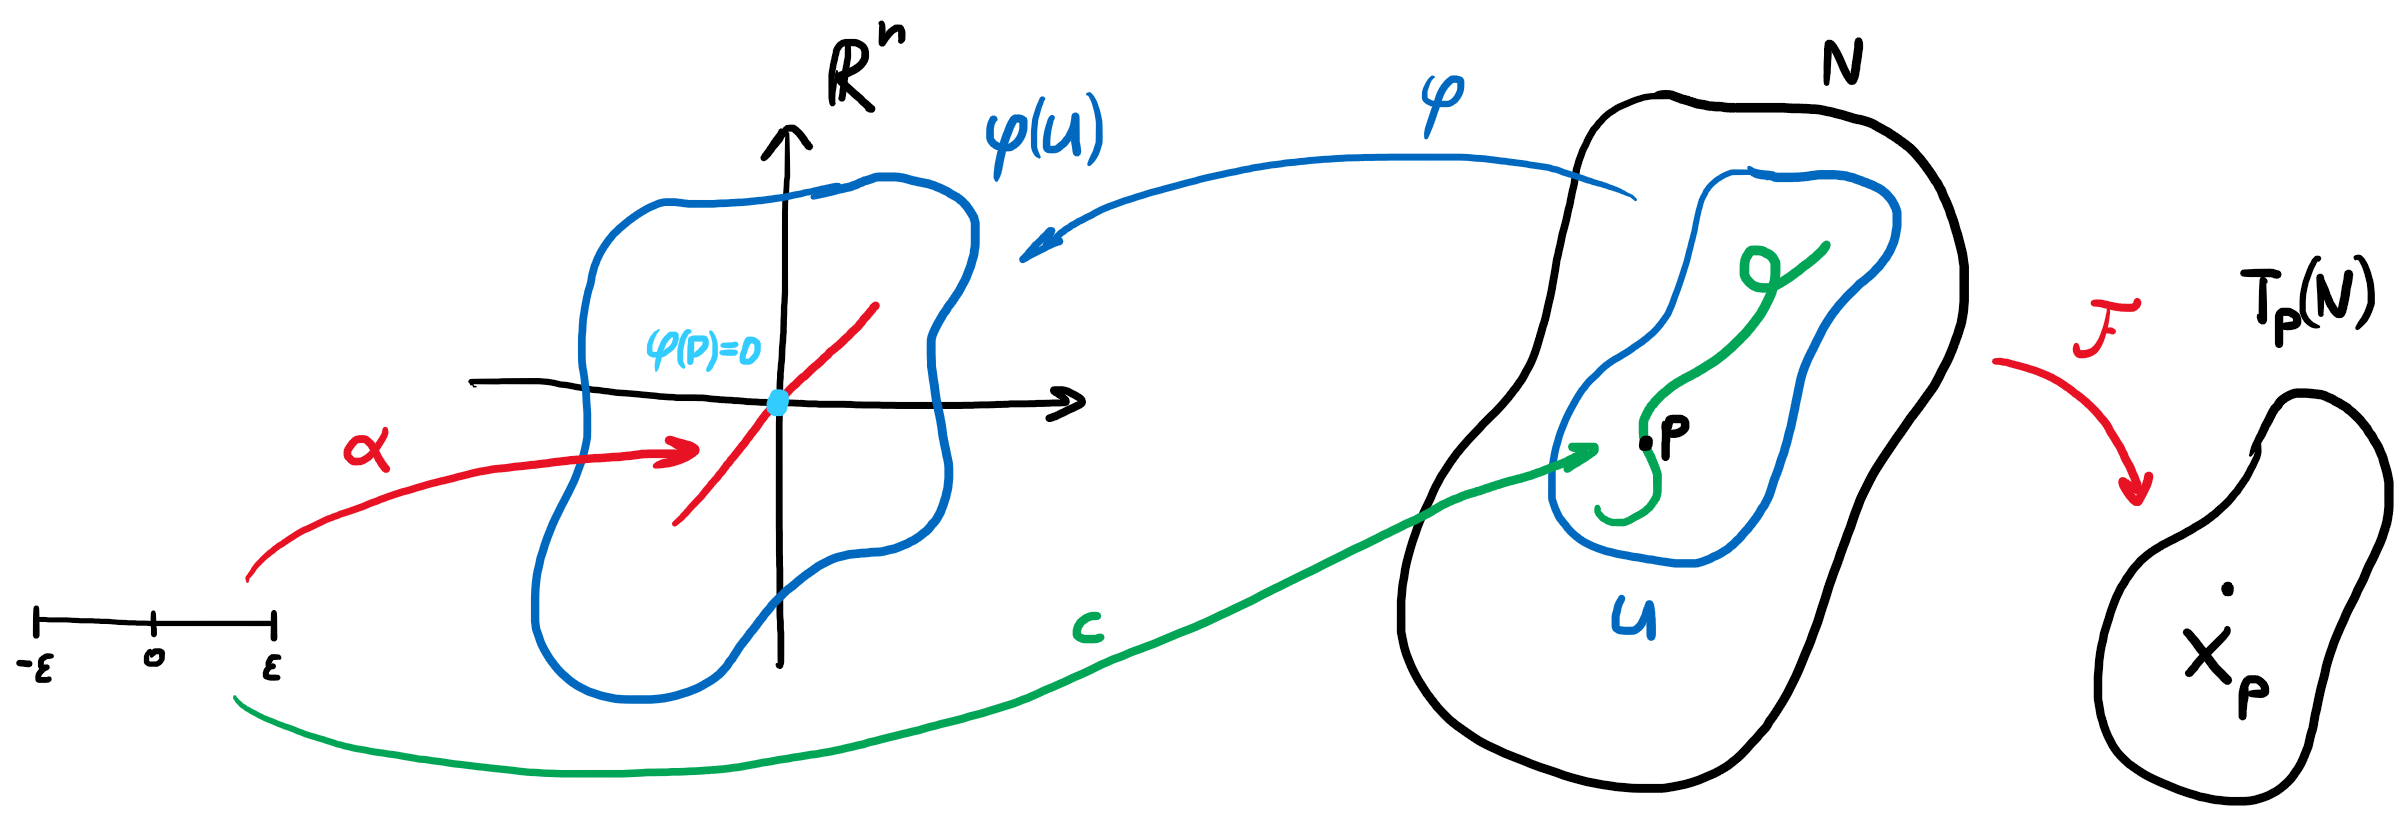
\includegraphics[width=0.7\textwidth,keepaspectratio]{img26}
	\end{figure}
\end{definition}

\begin{proof}
	\begin{align}
		\begin{split}
			F_{*p}(X_{p}) &= F_{*p}(c'(0))\\
			&= F_{*p} \left( c_{*0} \left( \left. \dfrac{\operatorname{d}}{\operatorname{dt}} \right|_{0} \right) \right)\\
			&= (F \circ c)_{*0} \left( \left. \dfrac{\operatorname{d}}{\operatorname{dt}} \right|_{0} \right)\\
			&= (F \circ c)' (0)
		\end{split}
	\end{align}

	in quanto $ c(0)=p $.
\end{proof}

\begin{corollary}
	Nel caso in cui lo spazio ambiente siano i numeri reali, i.e. $ M = \R $, sia $ f : N \to \R $ tale che $ f \in C^{\infty}(N) $ e $ X_{p} \in T_{p}(N) $, allora
	
	\begin{equation}
		f_{*p}(X_{p}) = (X_{p} f) \left. \dfrac{\operatorname{d}}{\operatorname{dr}} \right|_{f(p)}
	\end{equation}

	dove $ f_{*p} : T_{p}(N) \to T_{f(p)}(\R) $ e $ \langle \sfrac{\operatorname{d}}{\operatorname{dr}} |_{f(p)} \rangle = T_{f(p)}(\R) $.
\end{corollary}

\begin{proof}
	Sia $ c : (-\varepsilon,\varepsilon) \to N $ con $ c(0) = p $ una curva per il quale vale $ X_{p} = c'(0) $. Per le funzioni da $ \R $ in $ \R $ la composizione può essere scritta in funzione della derivata e, nel caso specifico di $ f \circ c : (-\varepsilon,\varepsilon) \to \R $, abbiamo
	
	\begin{equation}
		(f \circ c)'(0) = \dot{(f \circ c)}(0) \left. \dfrac{\operatorname{d}}{\operatorname{dr}} \right|_{f(p)}
	\end{equation}

	a questo punto
	
	\begin{align}
		\begin{split}
			f_{*p}(X_{p}) &= (f \circ c)' (0)\\
			&= \dot{(f \circ c)}(0) \left. \dfrac{\operatorname{d}}{\operatorname{dr}} \right|_{f(p)}\\
			&= (X_{p} f) \left. \dfrac{\operatorname{d}}{\operatorname{dr}} \right|_{f(p)}
		\end{split}
	\end{align}
\end{proof}

\subsubsection{\textit{Esempi}}

\paragraph{1. Differenziale della moltiplicazione per una matrice}\label{trasl-diff}

Consideriamo l'insieme delle matrici invertibili

\begin{equation}
	GL_{n}(\R) = \left\{ A \in M_{n}(\R) \, \middle| \, \det A \neq 0 \right\} \subset M_{n}(\R)
\end{equation}

il quale è un aperto di $ M_{n}(\R) = \R^{n^{2}} $ e inoltre è una varietà differenziabile di dimensione $ n^{2} $.\\
Fissata una matrice $ g \in GL_{n}(\R) $, definiamo l'applicazione

\begin{align}
	\begin{split}
		L_{g} : GL_{n}(\R) &\to GL_{n}(\R)\\
		h &\mapsto g h
	\end{split}
\end{align}

chiamata \textit{traslazione a sinistra tramite} $ g $. Questa applicazione è liscia, i.e. $ L_{g} \in C^{\infty} $.\\
L'obbiettivo è calcolare il differenziale di questa applicazione sulla matrice identità\footnote{%
	Considereremo il differenziale applicato alla matrice identità in quanto il differenziale è un'applicazione lineare.%
} $ I = I_{n} \in GL_{n}(\R) $

\begin{align}
	\begin{split}
		L_{g_{*I}} : T_{I}(GL_{n}(\R)) &\to T_{g}(GL_{n}(\R))\\
		X_{I} &\mapsto L_{g_{*I}}(X_{I})
	\end{split}
\end{align}

Innanzitutto, lo spazio di partenza è dato da

\begin{equation}
	T_{I}(GL_{n}(\R)) = \left\{ \sum_{i,j=1}^{n} X_{ij} \left. \dfrac{\partial}{\partial r_{ij}} \right|_{I} \, \middle| \, X=[X_{ij}] \in M_{n}(\R) \right\}
\end{equation}

dove $ \langle \sfrac{\partial}{\partial r_{ij}} |_{I} \rangle = T_{I}(GL_{n}(\R)) $; ad ogni vettore $ X_{I} \in T_{I}(GL_{n}(\R)) $ si può associare il vettore $ X \in M_{n}(\R) $ prendendo semplicemente $ X=[X_{ij}] $ dalla definizione dello spazio $ T_{I}(GL_{n}(\R)) $. Per quanto riguarda lo spazio di arrivo

\begin{equation}
	T_{g}(GL_{n}(\R)) = \left\{ \sum_{i,j=1}^{n} X_{ij} \left. \dfrac{\partial}{\partial r_{ij}} \right|_{g} \, \middle| \, X=[X_{ij}] \in M_{n}(\R) \right\}
\end{equation}

esattamente come per lo spazio di partenza, anche questo si identifica con $ M_{n}(\R) $.\\
Per calcolare il differenziale di $ L_{g} $, consideriamo una curva di matrici in $ GL_{n}(\R) $ il cui vettore tangente sia $ X_{I} $, i.e. $ c : (-\varepsilon,\varepsilon) \to GL_{n}(\R) $ con $ c(0)=I $ e 

\begin{equation}
	c'(0) = X_{I} = \sum_{i,j=1}^{n} X_{ij} \left. \dfrac{\partial}{\partial r_{ij}} \right|_{I}
\end{equation}

perciò

\begin{align}
	\begin{split}
		L_{g_{*I}}(X_{I}) &= (L_{g} \circ c)'(0)\\
		&= (g \, c(t))'(0)\\
		&= \sum_{i,j=1}^{n} \dot{(g \, c(t))}_{ij}(0) \left. \dfrac{\partial}{\partial r_{ij}} \right|_{g}
	\end{split}
\end{align}

dove $ g \, c(t) $ indica la moltiplicazione tra matrici e ricordando che un vettore tangente può essere scritto come

\begin{equation}
	c'(t_{0}) = \sum_{i=1}^{n} \dot{c}^{i}(t_{0}) \left. \dfrac{\partial}{\partial x^{i}} \right|_{t_{0}}
\end{equation}

considerando $ c : (a,b) \to N $ e $ (U,\phi) \in N $ con $ \phi=(x^{1},\dots,x^{n}) $ da cui $ c^{i} = x^{i} \circ c $.\\
Sappiamo che vale la regola di Leibniz per le matrici\footnote{%
	$ \dot{A(t) \, B(t)} = \dot{A}(t) \, B(t) + A(t) \, \dot{B}(t) \qquad \forall A(t),B(t) \in M_{n}(\R) $%
} e $ g $ non dipende da $ t $, dunque

\begin{align}
	\begin{split}
		L_{g_{*I}}(X_{I}) &= \sum_{i,j=1}^{n} \dot{(g \, c(t))}_{ij}(0) \left. \dfrac{\partial}{\partial r_{ij}} \right|_{g}\\
		&= \sum_{i,j=1}^{n} (g \, \dot{c}(0))_{ij} \left. \dfrac{\partial}{\partial r_{ij}} \right|_{g}\\
	\end{split}
\end{align}

Siccome

\begin{align}
	\begin{split}
		c'(0) &= X_{I}\\
		\sum_{i,j=1}^{n} \dot{c}(0)_{ij} \left. \dfrac{\partial}{\partial r_{ij}} \right|_{I} &= \sum_{i,j=1}^{n} X_{ij} \left. \dfrac{\partial}{\partial r_{ij}} \right|_{I}\\
		\dot{c}(0)_{ij} &= X_{ij}
	\end{split}
\end{align}

abbiamo che $ \dot{c}(0) = X = [X_{ij}] $ perciò

\begin{align}
	\begin{split}
		L_{g_{*I}}(X_{I}) &= \sum_{i,j=1}^{n} (g \, \dot{c}(0))_{ij} \left. \dfrac{\partial}{\partial r_{ij}} \right|_{g}\\
		&= \sum_{i,j=1}^{n} (g \, X)_{ij} \left. \dfrac{\partial}{\partial r_{ij}} \right|_{g}
	\end{split}
\end{align}

che può essere identificato naturalmente con la matrice $ g \, X $ quindi, tramite le identificazioni $ X_{I} \leftrightarrow X $ e $ L_{g_{*I}}(X_{I}) \leftrightarrow g \, X $, possiamo dunque scrivere

\begin{equation}
	L_{g_{*I}}(X) = g \, X
\end{equation}

Possiamo dunque affermare che il differenziale di $ L_{g} $ valutato nella matrice identità $ I $ corrisponde alla moltiplicazione a sinistra per $ g $.

\paragraph{2. Differenziale della moltiplicazione e dell'inversione in un gruppo di Lie}

Sia $ G $ un gruppo di Lie\footnote{%
	Se $ G $ è un gruppo di Lie, allora è una varietà differenziale e un gruppo algebrico con operazioni lisce
	
	\begin{align}
		\mu : G \times G &\to G & i : G &\to G\nonumber\\
		(g,h) &\mapsto g h & g &\mapsto g^{-1}
	\end{align}.%
} e $ e \in G $ l'identità. L'obbiettivo è calcolare i differenziali

\begin{align}
	\begin{split}
		\mu_{*(e,e)} &: T_{(e,e)}(G \times G) \to T_{e}(G)\\
		i_{*e} &: T_{e}(G) \to T_{e}(G)
	\end{split}
\end{align}

Sappiamo che\footnote{%
	Vedi Esercizio \ref{es2-11}.%
}, prese $ N $ e $ M $ due varietà differenziali con $ p \in N $ e $ q \in M $, si ha

\begin{equation}
	T_{(p,q)}(N \times M) \simeq T_{p}(N) \times T_{q}(M)
\end{equation}

Per calcolare $ \mu_{*(e,e)} $ prendiamo $ X_{e},Y_{e} \in \to T_{e}(G) $ e usiamo la curva liscia $ \gamma : (-\varepsilon,\varepsilon) \to G \times G $ con $ \gamma(0)=(e,e) $ e $ \gamma'(0) = (X_{e},Y_{e}) $. Sappiamo anche che

Inoltre sappiamo che il differenziale $ \mu_{*(e,e)} $ è lineare, dunque

\begin{equation}
	\mu_{*(e,e)}(X_{e},Y_{e}) = \mu_{*(e,e)}(X_{e},0) + \mu_{*(e,e)}(0,Y_{e})
\end{equation}

con $ 0 \in T_{e}(G) $. A questo punto, possiamo considerare i due addendi separatamente: prendiamo la curva liscia $ c : (-\varepsilon,\varepsilon) \to G $ con $ c(0)=e $ e $ c'(0) = X_{e} $, per il primo addendo

\begin{equation}
	\mu_{*(e,e)}(X_{e},0) = \mu(c(t),e)'(0)
\end{equation}

in quanto $ \gamma \doteq (c(t),e) $ è una curva per il quale vale $ \gamma(0) = (e,e) $ e $ \gamma'(0) = (c'(0),0) = (X_{e},0) $, ma $ \mu $ è la moltiplicazione dunque

\begin{align}
	\begin{split}
		\mu_{*(e,e)}(X_{e},0) &= \mu(c(t),e)'(0)\\
		&= (c(t) \, e)'(0)\\
		&= c'(0)\\
		&= X_{e}
	\end{split}
\end{align}

Il ragionamento è analogo per il secondo addendo, perciò

\begin{equation}
	\mu_{*(e,e)}(X_{e},Y_{e}) = X_{e} + Y_{e}
\end{equation}

Per quanto riguarda il differenziale dell'inversione $ i_{*e}(X_{e}) $ prendiamo ancora la curva liscia $ c : (-\varepsilon,\varepsilon) \to G $ con $ c(0)=e $ e $ c'(0) = X_{e} $ da cui

\begin{equation}
	i_{*e}(X_{e}) = (i \circ c)'(0)
\end{equation}

Se consideriamo la moltiplicazione tra la curva e la sua inversa, otteniamo

\begin{equation}
	\mu(c(t),i(c(t))) = e
\end{equation}

applicando il differenziale otteniamo

\begin{align}
	\begin{split}
		\mu(c(t),i(c(t))) &= e\\
		\mu_{*(e,e)}(c'(0),(i \circ c)'(0)) &= 0\\
		\mu_{*(e,e)}(X_{e},(i \circ c)'(0)) &= 0\\
		X_{e} + (i \circ c)'(0) &= 0\\
		(i \circ c)'(0) &= - X_{e}
	\end{split}
\end{align}

dunque

\begin{equation}
	i_{*e}(X_{e}) = - X_{e}
\end{equation}

\section{Immersioni, sommersioni e sottovarietà}

\subsection{Immersioni e sommersioni}

Un'applicazione liscia tra varietà $ F : N \to M $ è un'\textit{immersione} nel punto $ p \in N $ se il suo differenziale $ F_{*p} : T_{p}(N) \to T_{F(p)}(M) $ è iniettivo\footnote{%
	Equivalentemente $ \ker(F_{*p}) = \{0\} \in T_{p}(N) $.%
} mentre è una \textit{sommersione} in $ p $ se il suo differenziale $ F_{*p} : T_{p}(N) \to T_{F(p)}(M) $ è suriettivo.\\
Un'applicazione liscia $ F : N \to M $ è un'immersione (risp. una sommersione) se lo è in ogni $ p \in N $.

\begin{remark}
	Per i teoremi di algebra lineare\footnote{%
		Data un'applicazione lineare $ T : V \to W $, abbiamo che
		
		\begin{equation}
			\dim(V) + \dim(\ker(T)) = \dim(T(V))
		\end{equation}
		
		dove quest'ultimo viene anche chiamato rango di $ T $, i.e. $ \dim(T(V)) \doteq \rank(T) $.%
	}, se $ F : N \to M $ è un'immersione $ \dim(N) \leqslant \dim(M) $ mentre se è una sommersione $ \dim(N) \geqslant \dim(M) $.
\end{remark}

\begin{remark}
	Se $ F : N \to M $ è un'immersione e una sommersione in $ p $, i.e. $ \dim(N) = \dim(M) $ allora, per il teorema della funzione inversa\footnote{%
		Vedi Teorema \ref{ift}.%
	}, avremo che il differenziale è invertibile, dunque $ F $ è un diffeomorfismo locale intorno a $ p $.
\end{remark}

\begin{remark}
	In generale, un'immersione non è iniettiva e una sommersione non è suriettiva (lo sono necessariamente rispettivamente solo i loro differenziali).
\end{remark}

\subsubsection{\textit{Esempi}}

\paragraph{1. Immersione canonica}

Sia l'applicazione lineare (inclusione)

\begin{align}
	\begin{split}
		i : \R^{n} &\to \R^{m}\\
		(r^{1},\dots,r^{n}) &\mapsto (r^{1},\dots,r^{n},0,\dots,0)
	\end{split}
\end{align}

con $ n \leqslant m $ e con $ m-n $ zeri aggiunti nei punti dell'immagine.\\
Essendo lineare, il differenziale coincide con l'applicazione stessa, i.e. $ i_{*p} = i $, la quale è iniettiva, dunque $ i $ è un'immersione.\\
Questa applicazione definisce la forma canonica delle immersioni, cioè ogni immersione è localmente analoga all'inclusione sopra considerata\footnote{%
	Vedi Teorema \ref{loc-imm}.%
}.

\paragraph{2. Sommersione canonica}

Sia l'applicazione lineare (proiezione)

\begin{align}
	\begin{split}
		\pi : \R^{n} &\to \R^{m}\\
		(r^{1},\dots,r^{n}) &\mapsto (r^{1},\dots,r^{m})
	\end{split}
\end{align}

con $ n \geqslant m $.\\
Essendo lineare, il differenziale coincide con l'applicazione stessa, i.e. $ \pi_{*p} = \pi $, la quale è suriettiva, dunque $ \pi $ è una sommersione.\\
Questa applicazione definisce la forma canonica delle sommersioni, cioè ogni sommersione è localmente analoga alla proiezione sopra considerata\footnote{%
	Vedi Teorema \ref{loc-sub}.%
}.

\paragraph{3.}

Sia l'inclusione

\begin{align}
	\begin{split}
		i : U &\to N\\
		p &\mapsto p
	\end{split}
\end{align}

dove $ U \subset N $ aperto. Questa applicazione non è suriettiva se $ U \subsetneq N $ (è incluso ma non coincidente) ma il suo differenziale lo è, in quanto $ i_{*p} : T_{p}(U) = T_{p}(N) \to T_{p}(N) $ corrisponde all'identità (è anche iniettivo).\\
Dunque l'inclusione considerata non è suriettiva ma è un'immersione e una sommersione.

\subsubsection{Rango di un'applicazione liscia}

Siano $ F : N \to M $ un'applicazione liscia, $ p \in N $ e $ (U,\phi) \in N $ con $ \phi = (x^{1},\dots,x^{n}) $ e $ (V,\psi) \in M $ con $ \psi = (y^{1},\dots,y^{m}) $ carte intorno a $ p $ e $ F(p) $ rispettivamente, tale che $ F(U) \subseteq V $. Definiamo il \textit{rango} di $ F $ nel punto $ p $ come

\begin{equation}
	\rank(F(p)) \doteq \rank\left( \left[ \dfrac{\partial F^{i}}{\partial x^{j}} (p) \right] \right) \equiv \rank(F_{*p})
\end{equation}

dove $ F^{i} = y^{i} \circ F = r^{i} \circ \psi \circ F $, in quanto la matrice di $ F_{*p} $ rispetto alle basi

\begin{align}
	\begin{split}
		\mathcal{B}_{T_{p}(N)} &= \left( \left. \dfrac{\partial}{\partial x^{1}} \right|_{p} , \dots , \left. \dfrac{\partial}{\partial x^{n}} \right|_{p} \right)\\
		\mathcal{B}_{T_{F(p)}(M)} &= \left( \left. \dfrac{\partial}{\partial y^{1}} \right|_{F(p)} , \dots , \left. \dfrac{\partial}{\partial y^{m}} \right|_{F(p)} \right)
	\end{split}
\end{align}

è proprio lo jacobiano di $ F $ nel punto $ p $ associato alle carte definite sopra, i.e.

\begin{equation}
	J(F(p)) = \left[ \dfrac{\partial F^{i}}{\partial x^{j}} (p) \right] \in M_{m,n}(\R)
\end{equation}

Il rango di un'applicazione liscia definito in questo modo è ben definito in quanto lo è quello di un'applicazione lineare: il rango della matrice associata non dipende dalle basi scelte per calcolare la matrice stessa perché due matrici ottenute a partire da due basi diverse differiscono tra loro per la moltiplicazione di una matrice invertibile.

\begin{remark}
	Se $ F $ è un'immersione in $ p $, allora $ \rank(F(p)) = n \leqslant m $ mentre se è una sommersione $ \rank(F(p)) = m \leqslant n $, in entrambi casi il rango è massimo.
\end{remark}

\subsection{Punti e valori critici e regolari}

Sia $ F : N \to M $ un'applicazione liscia, un punto $ p \in N $ è un \textit{punto critico per} $ F $ se il differenziale $ F_{*p} : T_{p}(N) \to T_{F(p)}(M) $ non è suriettivo mentre $ p \in N $ è un \textit{punto regolare per} $ F $ se il differenziale è suriettivo (equivalentemente $ F $ è una sommersione in $ p $).\\
I punti critici e regolari appartengono al dominio della funzione.\\
Come notazione

\begin{align}
	\begin{split}
		\mathcal{PC}_{F} &= \{ p \in N \mid p \text{ punto critico per } F \} \subset N\\
		\mathcal{PR}_{F} &= \{ p \in N \mid p \text{ punto regolare per } F \} \subset N
	\end{split}
\end{align}

dove valgono

\begin{equation}
	\begin{cases}
		N = \mathcal{PC}_{F} \cup \mathcal{PR}_{F}\\
		\mathcal{PC}_{F} \cap \mathcal{PR}_{F} = \{\}
	\end{cases}
\end{equation}

Consideriamo l'insieme dei punti di $ N $ che hanno come immagine $ q \in M $ attraverso $ F $, i.e.

\begin{equation}
	F^{-1}(q) = \{ p \in N \mid F(p) = q \}
\end{equation}

Un punto $ q \in M $ è un \textit{valore regolare per} $ F $ se ogni punto $ p \in F^{-1}(q) $ è un punto regolare. Un punto $ q \in M $ è un \textit{valore critico per} $ F $ se non è un valore regolare o, equivalentemente, se esiste un punto $ p \in F^{-1}(q) $ tale che $ p $ sia un punto critico.\\
I punti critici e regolari appartengono al dominio della funzione.\\
Come notazione

\begin{align}
	\begin{split}
		\mathcal{VR}_{F} &= \{ q \in M \mid q \text{ valore regolare per } F \} \subset M\\
		\mathcal{VC}_{F} &= \{ q \in M \mid q \text{ valore critico per } F \} \subset M
	\end{split}
\end{align}

Perciò possiamo scrivere che

\begin{align}
	\begin{split}
		q \in \mathcal{VR}_{F} &\iff p \in \mathcal{PR}_{F}, \, \forall p \in F^{-1}(q)\\
		q \in \mathcal{VC}_{F} &\iff \E p \in F^{-1}(q) \mid p \in \mathcal{PC}_{F}
	\end{split}
\end{align}

Analogamente ai punti regolari e critici, valgono le seguenti relazioni

\begin{equation}
	\begin{cases}
		M = \mathcal{VC}_{F} \cup \mathcal{VR}_{F}\\
		\mathcal{VC}_{F} \cap \mathcal{VR}_{F} = \{\}
	\end{cases}
\end{equation}

\begin{remark}
	Se $ q \in M $ ma $ q \notin F(N) $ allora $ q $ è un valore regolare, i.e.
	
	\begin{equation}
		M \setminus F(N) \subset \mathcal{VR}_{F}
	\end{equation}
\end{remark}

\begin{remark}
	\begin{equation}
		F(\mathcal{PC}_{F}) = \mathcal{VC}_{F}
	\end{equation}

	ma in generale
	
	\begin{equation}
		F(\mathcal{PR}_{F}) \not\subset \mathcal{VR}_{F} \wedge F(\mathcal{PR}_{F}) \not\supset \mathcal{VR}_{F}
	\end{equation}
\end{remark}

\subsubsection{Codominio $ \R $}

Nel caso in cui $ M = \R $, consideriamo la funzione liscia $ f : N \to \R $.\\
Se $ p \in \mathcal{PC}_{f} $ allora $ f_{*p} : T_{p}(N) \to T_{f(p)}(\R) $ non è suriettivo: perché il differenziale non sia suriettivo, essendo $ \dim(T_{f(p)}(\R)) = 1 $, è necessario che $ f_{*p} = 0 $ o, equivalentemente, che l'immagine di $ f_{*p} $ sia l'insieme nullo, i.e.

\begin{equation}
	f_{*p}(T_{p}(N)) = \{0\}
\end{equation}

Questo significa che

\begin{equation}
	f_{*p}(X_{p}) = 0 \in T_{f(p)}(\R)
\end{equation}

per $ \forall X_{p} \in T_{p}(N) $ e sappiamo che

\begin{equation}
	f_{*p}(X_{p}) = (X_{p} f) \left. \dfrac{\operatorname{d}}{\operatorname{dr}} \right|_{f(p)}
\end{equation}

dove $ X_{p} f \in \R $ e $ \langle \sfrac{\operatorname{d}}{\operatorname{dr}} |_{f(p)} \rangle = T_{f(p)}(\R) $.\\
Sia la carta $ (U,\phi) \in N $ con $ \phi = (x^{1},\dots,x^{n}) $ intorno a $ p $, allora

\begin{equation}
	X_{p} = \sum_{i=1}^{n} a^{i} \left. \dfrac{\partial}{\partial x^{i}} \right|_{p}
\end{equation}

dunque

\begin{equation}
	X_{p} f = \sum_{i=1}^{n} a^{i} \dfrac{\partial f}{\partial x^{i}} (p)
\end{equation}

Perché $ f_{*p}(X_{p}) = 0 $ è necessario che $ X_{p} f = 0 $, il che implica

\begin{equation}
	\dfrac{\partial f}{\partial x^{i}} (p) = 0
\end{equation}

per $ \forall i=1,\dots,n $.\\
Riassumendo, la condizione per cui un punto $ p \in N $ sia un punto critico è la seguente

\begin{gather}
	p \in \mathcal{PC}_{f}\nonumber\\
	\Updownarrow\\
	\dfrac{\partial f}{\partial x^{i}} (p) = 0, \, \forall i=1,\dots,n \wedge \forall (U,\phi) \in N \mid \phi = (x^{1},\dots,x^{n}) \wedge p \in (U,\phi)\nonumber
\end{gather}

In particolare, se $ N = (a,b) $, la condizione per cui un punto $ t_{0} \in (a,b) $ sia un punto critico è

\begin{equation}
	t_{0} \in \mathcal{PC}_{f} \iff \dot{f}(t_{0}) = 0
\end{equation}

\subsubsection{\textit{Esempi}}

\paragraph{1.}

Sia la funzione

\begin{align}
	\begin{split}
		f : \R &\to \R\\
		x &\mapsto x^{4} - 2 x^{2}
	\end{split}
\end{align}

\begin{figure}[H]
	\centering
	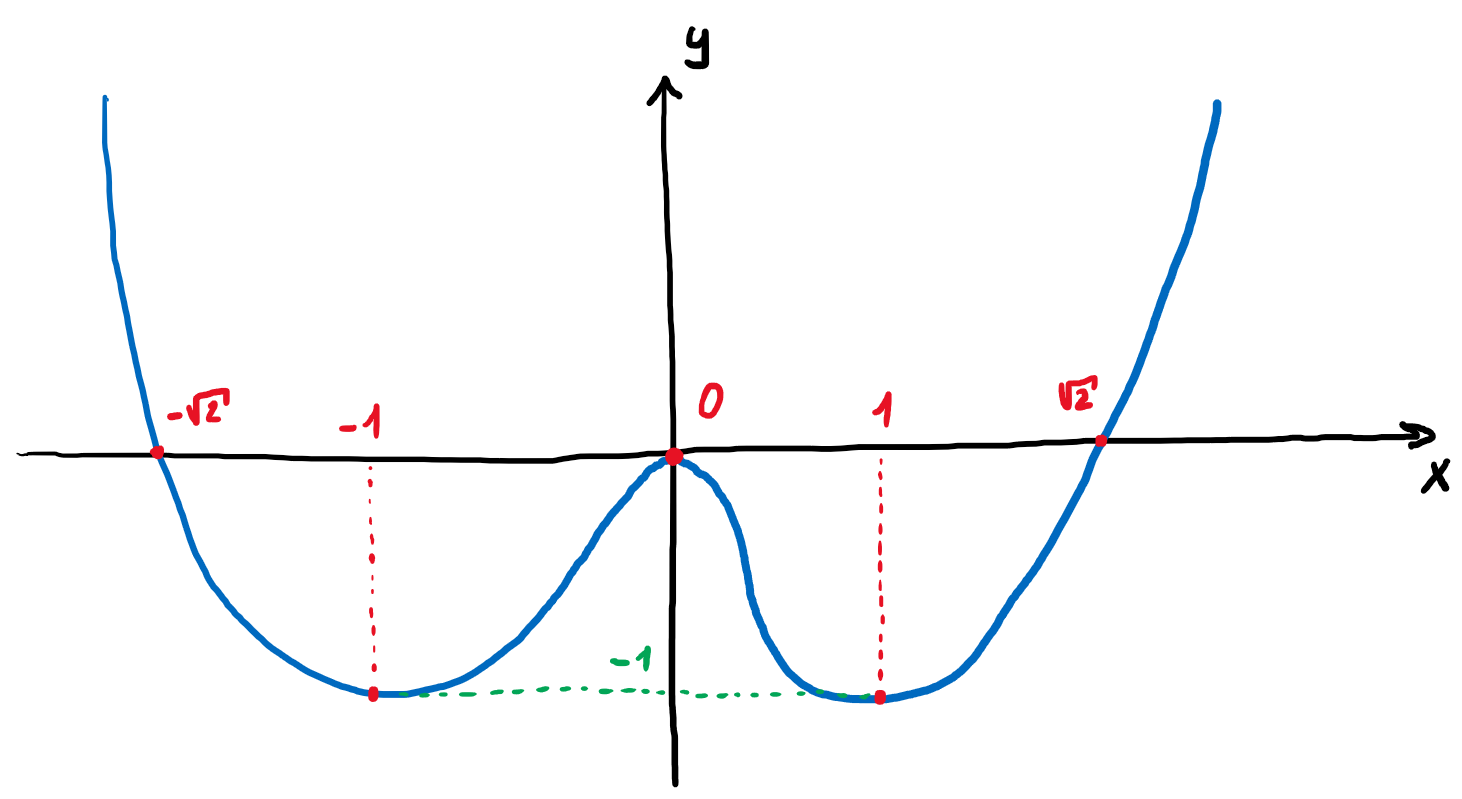
\includegraphics[width=0.6\textwidth,keepaspectratio]{img28}
\end{figure}

Abbiamo che

\begin{equation}
	\begin{cases}
		\mathcal{PC}_{f} = \{ x \in \R \mid \dot{f}(x) = 4 x^{3} - 4 x = 0 \} = \{ -1, 0, 1 \}\\
		\mathcal{PR}_{f} = \R \setminus \mathcal{PC}_{f} = \R \setminus \{ -1, 0, 1 \}\\
		\mathcal{VC}_{f} = f(\mathcal{PC}_{f}) = \{ -1, 0 \}\\
		\mathcal{VR}_{f} = \R \setminus \mathcal{VC}_{f} = \R \setminus \{ -1, 0 \}
	\end{cases}
\end{equation}

Sappiamo inoltre che $ f(\mathcal{PR}_{f}) \not\subset \mathcal{VR}_{f} $ in quanto, ad esempio, $ \sqrt{2} \in \mathcal{PR}_{f} $ ma $ f(\sqrt{2}) = 0 \notin \mathcal{VC}_{f} $.

\paragraph{2.}

Sia $ F : N \to M $ un'applicazione lisca non suriettiva. Per qualunque $ q \in M \setminus F(N) $ abbiamo che $ q \in \mathcal{VR}_{F} $ per definizione ma $ q \notin F(\mathcal{PR}_{F}) $ in quanto $ q \notin F(N) $.\\
Riassumendo $ F(\mathcal{PR}_{F}) \not\supset \mathcal{VR}_{F} $.

\subsubsection{Massimi e minimi relativi}

In analisi, per una funzione $ f : \R \to \R $ il punto $ x_{0} \in \R $ è un massimo (risp. minimo) locale se esiste un intorno $ I $ contenente $ x_{0} $ tale che $ f(x) \leqslant f(x_{0}) $ (risp. $ f(x) \geqslant f(x_{0}) $) per $ \forall x \in I $. Se $ x_{0} $ è un punto di massimo o minimo relativo allora\footnote{%
	Per definizione
	
	\begin{equation}
		\dot{f}(x_{0}) = \lim_{x \to x_{0}} \dfrac{f(x) - f(x_{0})}{x - x_{0}}
	\end{equation}

	Per un massimo locale $ f(x) \leqslant f(x_{0}) $ per $ \forall x \in I $ dunque $ f(x) - f(x_{0}) \leqslant 0 $; considerando i limiti da destra e da sinistra e sfruttando la permanenza del segno
	
	\begin{align}
		\begin{split}
			\dot{f}(x_{0})^{+} = \lim_{x \to x_{0}^{+}} \dfrac{f(x) - f(x_{0})}{x - x_{0}} \leqslant 0\\
			\dot{f}(x_{0})^{-} = \lim_{x \to x_{0}^{-}} \dfrac{f(x) - f(x_{0})}{x - x_{0}} \geqslant 0
		\end{split}
	\end{align}

	perciò $ \dot{f}(x_{0}) = 0 $.%
} $ \dot{f}(x_{0}) = 0 $, dunque $ x_{0} \in \mathcal{PC}_{f} $.\\\\
%
Sia $ N $ una varietà differenziabile e $ f \in C^{\infty}(N) $, un punto $ p \in N $ è un \textit{massimo locale} (risp. \textit{minimo locale}) per $ f $ se esiste un intorno $ U \in N $ di $ p $ tale che $ f(q) \leqslant f(p) $ (risp. $ f(q) \geqslant f(p) $ ) per $ \forall q \in U $.

\begin{definition}
	Se $ p $ è un punto di massimo locale (risp. minimo locale) per $ f $ allora $ p \in \mathcal{PC}_{f} $.
\end{definition}

\begin{proof}
	Ricordiamo che
	
	\begin{gather}
		p \in \mathcal{PC}_{f}\nonumber\\
		\Updownarrow\nonumber\\
		\dfrac{\partial f}{\partial x^{i}} (p) = 0, \, \forall i=1,\dots,n \wedge \forall (U,\phi) \in N \mid \phi = (x^{1},\dots,x^{n}) \wedge p \in (U,\phi)\nonumber\\
		\Updownarrow\\
		f_{*p}(X_{p}) = 0, \, \forall X_{p} \in T_{p}(N)\nonumber
	\end{gather}

	con
	
	\begin{equation}
		f_{*p}(X_{p}) = (X_{p} f) \left. \dfrac{\operatorname{d}}{\operatorname{dr}} \right|_{f(p)}
	\end{equation}

	La derivata direzionale si può calcolare usando curve su varietà, dunque presa $ c : (-\varepsilon,\varepsilon) \to N $ con $ c(0) = p $ e $ c'(0) = X_{p} $ abbiamo che
	
	\begin{equation}
		X_{p} f = \dot{(f \circ c)}(0)
	\end{equation}

	quindi
	
	\begin{equation}
		f_{*p}(X_{p}) = \dot{(f \circ c)}(0)
	\end{equation}

	\begin{figure}[H]
		\centering
		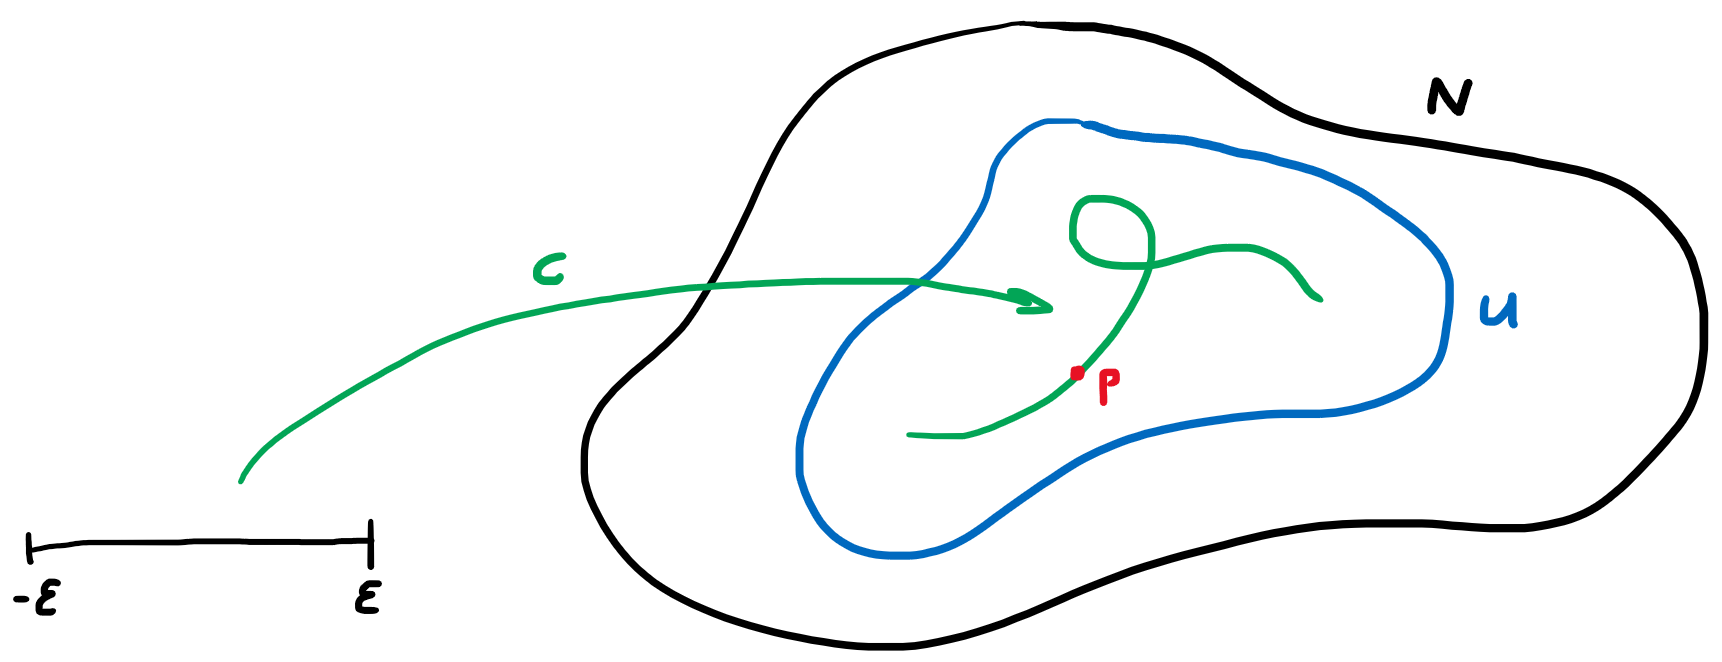
\includegraphics[width=0.6\textwidth,keepaspectratio]{img29}
	\end{figure}
	
	Sappiamo che $ f(q) \leqslant f(p) $ per $ \forall q \in U $ intorno, quindi prendiamo $ \varepsilon $ in modo tale che $ c((-\varepsilon,\varepsilon)) \subset U $. Se $ p $ è un massimo locale per $ f $ allora 0 è un massimo locale per $ f \circ c $ cioè
	
	\begin{equation}
		(f \circ c)(t) \leqslant (f \circ c)(0) = f(p), \, \forall t \in (-\varepsilon,\varepsilon)
	\end{equation}

	Dall'analisi otteniamo che $ \dot{(f \circ c)}(0) = 0 $ dunque $ f_{*p}(X_{p}) = 0 $ e perciò $ p \in \mathcal{PC}_{f} $.\\	
	La dimostrazione per il minimo locale è analoga.
\end{proof}

\subsubsection{Matrice hessiana}

Sia $ N $ una varietà compatta dove $ \dim(N)=2 $. Un punto $ p \in N $  è detto punto critico \textit{non degenere} se $ p \in \mathcal{PC} $ e se, presa una carta $ (U\,\phi) $ con $ \phi (x^{1},x^{2}) $, il determinante della \textit{matrice hessiana} associata a $ f $ in $ p $ è diverso da zero, i.e.

\begin{equation}
	\det(\mathcal{H}(f)(p)) \doteq \det (\begin{bmatrix} \dfrac{\partial^{2} f}{\partial (x^{1})^{2}} & \dfrac{\partial^{2} f}{\partial x^{1} \partial x^{2}} \\\\ \dfrac{\partial^{2} f}{\partial x^{2} \partial x^{1}} & \dfrac{\partial^{2} f}{\partial (x^{2})^{2}} \end{bmatrix}) \neq 0
\end{equation}

La maggior parte delle funzioni possiedono punti critici non degeneri.\\
Analogamente come in analisi, si possono classificare i punti critici non degeneri in base alla loro matrice hessiana:

\begin{itemize}
	\item $ \mathcal{H}(f)(p) < 0 \text{ definita negativa} \implies p \text{ massimo locale} $
	
	\item $ \mathcal{H}(f)(p) > 0 \text{ definita positiva} \implies p \text{ minimo locale} $
	
	\item $ \mathcal{H}(f)(p) \gtreqqless 0 \text{ semidefinita} \implies p \text{ punto di sella} $
\end{itemize}

Ad esempio, il paraboloide $ z^{2} = - x^{2} - y^{2} $ ha come massimo locale il punto $ (0,0) $, per la funzione

\begin{align}
	\begin{split}
		f : \R^{2} &\to \R\\
		(x,y) &\mapsto - x^{2} - y^{2}
	\end{split}
\end{align}

dove

\begin{equation}
	\mathcal{H}(f)(p) = \begin{bmatrix} -2 & 0 \\ 0 & -2 \end{bmatrix} < 0
\end{equation}

Il paraboloide $ z^{2} = x^{2} + y^{2} $ ha $ (0,0) $ come minimo locale mentre il paraboloide iperbolico $ z^{2} = x^{2} - y^{2} $ ha $ (0,0) $ come punto di sella.

\subsubsection{Teoria di Morse}

La teoria di Morse lega lo studio dei punti critici di una varietà alla sua topologia.

\begin{theorem}[Morse per superfici]
	Siano $ N $ una varietà compatta e connessa con $ \dim(N)=2 $ e $ f $ una funzione liscia che ha tutti i punti critici non degeneri. Siano
	
	\begin{itemize}
		\item $ M = \# \{ \text{punti di massimo per } f \} $
		
		\item $ m = \# \{ \text{punti di minimo per } f \} $
		
		\item $ s = \# \{ \text{punti di sella per } f \} $
	\end{itemize}

	i quali sono finiti perché la varietà è compatta.\\
	Allora
	
	\begin{equation}
		M - s + m = \chi(N)
	\end{equation}

	dove $ \chi(N) $ è la \textit{caratteristica di Eulero} della superficie $ N $. La caratteristica di Eulero è data da
	
	\begin{equation}
		\chi(N) = F - L + V
	\end{equation}

	dove $ F $ sono le facce, $ L $ sono i lati e $ V $ sono i vertici che compaiono nella suddivisione di una varietà compatta in triangoli (curvilinei).
\end{theorem}

Questo teorema si generalizza a $ n $ dimensioni.\\
Ad esempio, consideriamo il toro $ \T^{2} $ e la funzione "altezza" $ f : \T^{2} \to \R $ la quale ha come immagine del toro l'altezza dei punti dello stesso:

\begin{figure}[H]
	\centering
	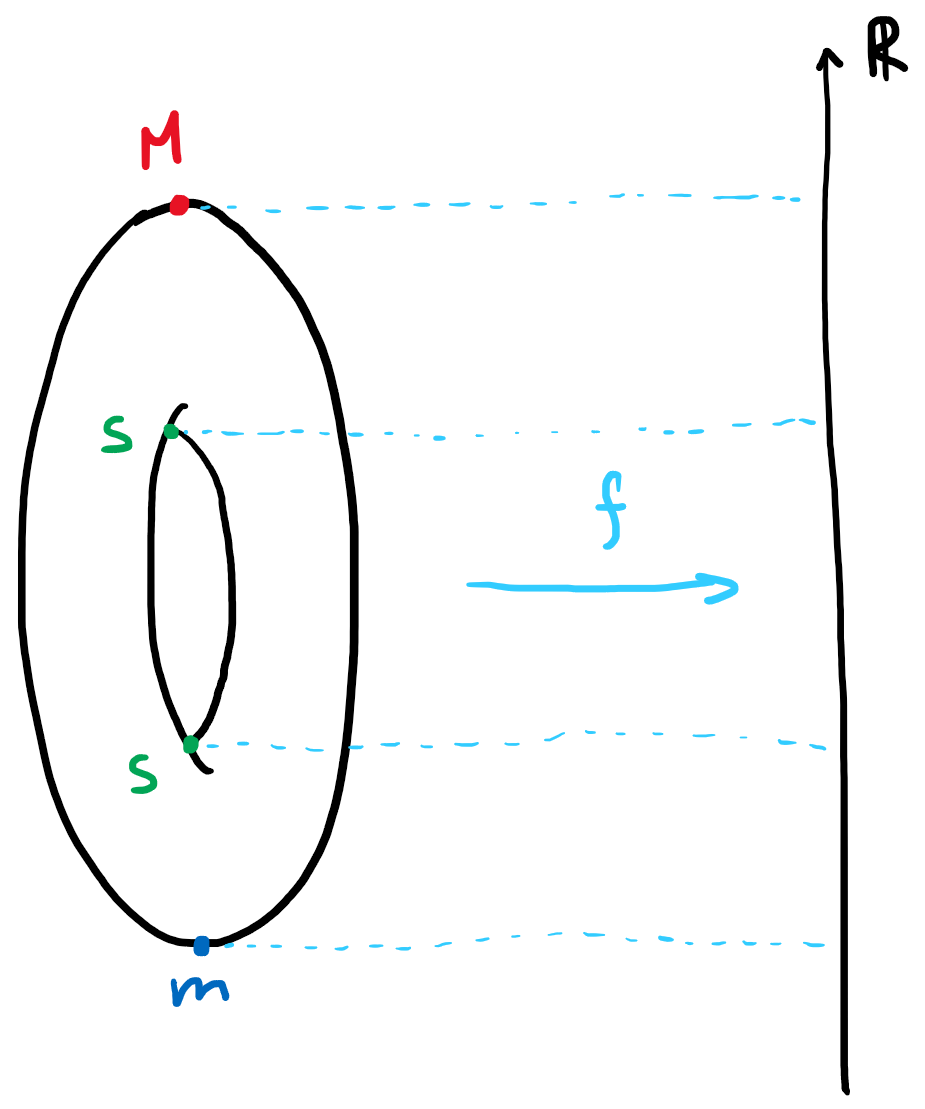
\includegraphics[width=0.3\textwidth,keepaspectratio]{img30}
\end{figure}

La caratteristica di Eulero del toro è

\begin{equation}
	\chi(\T^{2}) = 1-2+1 = 0
\end{equation}

Se consideriamo la sfera $ \S^{2} $ tramite la funzione altezza, otteniamo

\begin{equation}
	\chi(\S^{2}) = 1-0+1 = 2
\end{equation}

In generale, per una varietà compatta di dimensione due, la quale è diffeomorfa alla superficie con $ g $ buchi $ \Sigma_{g} $, usando la funzione altezza

\begin{figure}[H]
	\centering
	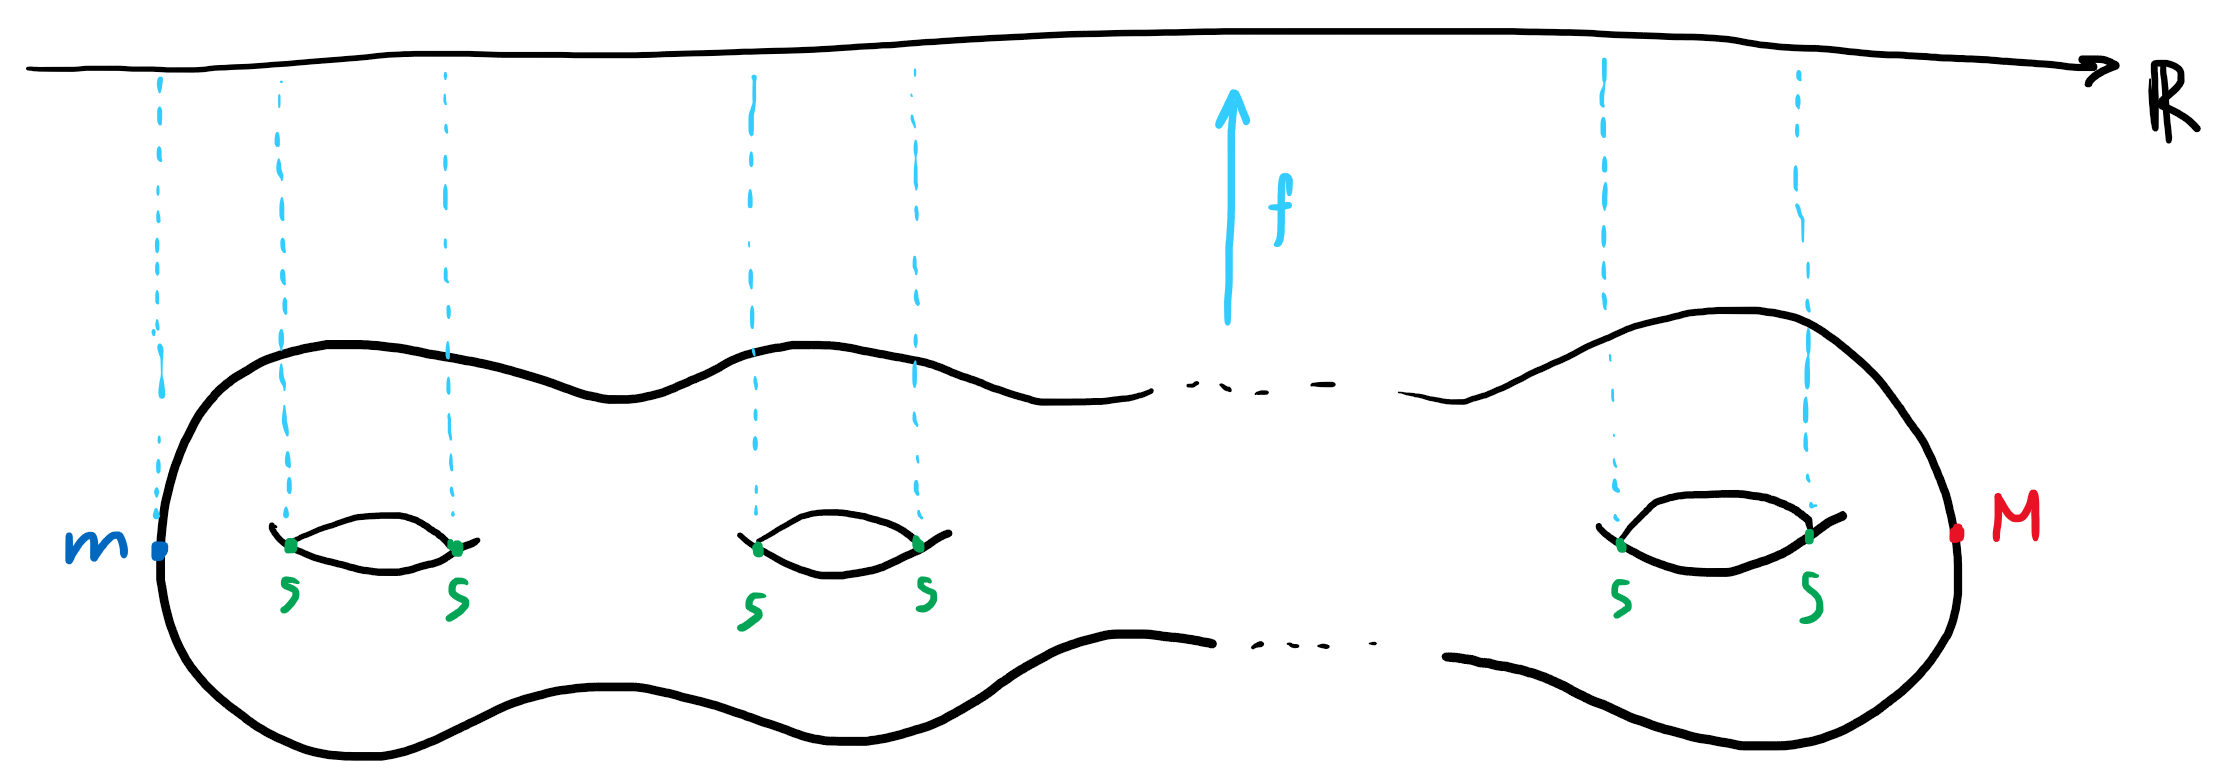
\includegraphics[width=0.5\textwidth,keepaspectratio]{img31}
\end{figure}

La sua caratteristica di Eulero è dunque

\begin{equation}
	\chi(\Sigma_{g}) = 1-2g+1 = 2 (1-g)
\end{equation}

\subsection{Sottovarietà}

Siano $ N $ una varietà differenziabile con $ \dim(N)=n $ e $ S \subset N $ sottospazio topologico di $ N $ (con la topologia indotta da $ N $), allora $ S $ è una \textit{sottovarietà di} $ N $ di dimensione $ \dim(S) = k \leqslant n $ se per ogni punto $ p \in S $ esiste una carta $ (U,\phi) $ con $ \phi = (x^{1},\dots,x^{n}) $ intorno a $ p $ tale che l'aperto $ U \cap S $ sia costituito dai punti di $ U $ che abbiano le ultime $ n-k $ funzioni coordinate nulle\footnote{%
	Due carte che hanno le stesse coordinate ma invertite sono identiche, i.e. $ (U;x^{1},x^{2}) \equiv (U;x^{2},x^{1}) $.%
}, i.e.

\begin{gather}
	S \text{ sottovarietà}\nonumber\\
	\Downarrow\\
	\forall p \in S, \, \E (U,\phi) \in N \mid (U,\phi) \ni p \wedge U \cap S = \{ q \in U \mid x^{k+1}(q) = \dots = x^{n}(q) = 0 \}\nonumber
\end{gather}

Ad esempio, se consideriamo $ N = \R^{2} $ con carta $ (x,y) $ e $ S = \R \times \{0\} $ allora

\begin{equation}
	\R^{2} \cap S = S = \{ (x,y) \in \R^{2} \mid y=0 \}
\end{equation}

mentre per $ N = \R^{3} $ con carta $ (x,y,z) $ e $ S = \R \times \{0\} $ allora

\begin{equation}
	\R^{3} \cap S = S = \{ (x,y,z) \in \R^{2} \mid y=0 \wedge z=0 \}
\end{equation}

\begin{remark}\label{subvar-open}
	Sia $ S \subset N $ un aperto di una varietà $ N $ con $ \dim(N)=n $, allora $ S $ è una sottovarietà di $ N $ con $ \dim(S)=n $.\\
	Questo è vero in quanto, presa una carta $ (U,\phi) \in N $, la condizione
	
	\begin{equation}
		U \cap S = \{ q \in U \mid x^{k+1}(q) = \dots = x^{n}(q) = 0 \}
	\end{equation}

	si verifica per $ k=n $, i.e. 0 coordinate si annullano in $ U \cap S $.\\
	Ad esempio, non potrebbe essere che
	
	\begin{equation}
		U \cap S = \{ q \in U \mid x^{i}(q) = 0 \}
	\end{equation}

	in quanto $ U \simeq \R^{n} $ tramite $ \phi $, $ U \cap S \simeq \R^{n-1} $ e $ U \cap S \simeq U $ ma i diffeomorfismi conservano la dimensione.
\end{remark}

Siano $ N $ una varietà differenziabile con $ \dim(N)=n $, $ S \subset N $ una sottovarietà con $ \dim(S)=k $ e $ p \in S $, allora una carta $ (U,\phi) \in N $ con $ \phi = (x^{1},\dots,x^{n}) $ tale che $ (U,\phi) \ni p $ è chiamata \textit{carta adattata di} $ N $ \textit{intorno a} $ p $ \textit{relativamente a} $ S $ se vale la condizione per la sottovarietà, i.e.

\begin{equation}
	U \cap S = \{ q \in U \mid x^{k+1}(q) = \dots = x^{n}(q) = 0 \}
\end{equation}

\subsubsection{\textit{Esempi}}

\paragraph{1.}

Consideriamo $ N = \R^{2} $ con carta $ U = (-1,1) \times (-1,1) $ (quadrato di lato 2) e $ S = (-1,1) \times \{0\} $. La carta $ U $ è adattata relativamente a $ S $ in quanto

\begin{equation}
	U \cap S = \{ q \in U \mid y(q) = 0 \} = S
\end{equation}

\paragraph{2.}

Consideriamo $ N = \R^{2} $ con carta $ V = (0,2) \times (-1,1) $ (quadrato di lato 2 decentrato verso destra) e $ S = (-1,1) \times \{0\} $. La carta $ V $ non è adattata relativamente a $ S $ in quanto

\begin{gather}
	V \cap S = (0,1) \times \{0\}\nonumber\\
	\neq\\
	\{ q \in V \mid y(q) = 0 \} = (0,2) \times \{0\}\nonumber
\end{gather}

\paragraph{3.}

Consideriamo $ N = \R^{n} $ con carta $ (U,\phi) = (\R;r^{1},\dots,r^{n}) $ e $ S = \R^{k} \times \{0\} \subset N $. La carta $ (U,\phi) $ è una carta adattata intorno ad ogni punto $ p \in S $ relativamente ad $ S $ in quanto

\begin{equation}
	U \cap S = S = \{ q \in \R^{n} \mid r^{k+1}(q) = \dots = r^{n}(q) = 0 \}
\end{equation}

\subsubsection{Sottovarietà come varietà differenziabile}

Osserviamo che se definiamo

\begin{align}
	\begin{split}
		\phi_{S} : U \cap S &\to \R^{k}\\
		q &\mapsto (x^{1}(q),\dots,x^{k}(q))
	\end{split}
\end{align}

dove $ (U,\phi) $ è una carta adattata di $ N $ intorno a $ p $ relativamente a $ S $, come la restrizione della funzione

\begin{align}
	\begin{split}
		\phi_{| U \cap S} : U \cap S &\to \R^{n}\\
		q &\mapsto (x^{1}(q),\dots,x^{k}(q),0,\dots,0)
	\end{split}
\end{align}

Siccome $ \phi $ è un omeomorfismo, allora lo è anche $ \phi_{S} $ in quanto restrizione di un omeomorfismo.\\
Deduciamo dunque che $ S $ è una varietà topologica con $ \dim(S)=k $ poiché $ S $ è $ N_{2}+T_{2} $ dal fatto che $ S \subset N $ sottospazio e inoltre per $ \forall p \in S $ si può definire una carta $ (U \cap S,\phi_{S}) $ intorno a $ p $ dal quale si ottiene un atlante topologico per $ S $.

\begin{definition}
	Sia $ S $ una sottovarietà con $ \dim(S)=k $ di una varietà differenziabile $ N $ con $ \dim(N)=n $, allora $ S $ è una varietà differenziabile con $ \dim(S)=k $.\\
	Chiameremo la struttura differenziabile costruita nella proposizione la \textit{struttura differenziale indotta da} $ N $.
\end{definition}

\begin{proof}
	Per dimostrare che $ S $ sia una varietà differenziabile, dobbiamo far vedere che per $ \forall p \in S $ e per $ \forall (U \cap S,\phi_{S}),(V \cap S,\psi_{S}) $ carte indotte da carte adattate $ (U,\phi) $ e $ (V,\psi) $ allora $ (U \cap S,\phi_{S}) $ è $ C^{\infty} $-compatibile con $ (V \cap S,\psi_{S}) $.\\
	Sia la carta adattata $ (U,\phi) $ con $ \phi = (x^{1},\dots,x^{n}) $ tale che
	
	\begin{equation}
		U \cap S = \{ q \in U \mid x^{k+1}(q) = \dots = x^{n}(q) = 0 \}
	\end{equation}

	e analogamente $ (V,\psi) $ con $ \psi = (y^{1},\dots,y^{n}) $ tale che
	
	\begin{equation}
		V \cap S = \{ q \in V \mid y^{k+1}(q) = \dots = y^{n}(q) = 0 \}
	\end{equation}

	Essendo $ (U,\phi) $ e $ (V,\psi) $ carte di $ N $ queste sono $ C^{\infty} $-compatibili, i cambi di carta
	
	\begin{align}
		\begin{split}
			\psi \circ \phi^{-1} &: \phi(U \cap V) \to \psi(U \cap V)\\
			\phi \circ \psi^{-1} &: \psi(U \cap V) \to \phi(U \cap V)
		\end{split}
	\end{align}

	sono lisci, quindi abbiamo le loro applicazioni su coordinate euclidee
	
	\begin{align}
		\begin{split}
			(\psi \circ \phi^{-1}) (\, (\, r^{1}(\phi(q)),\dots,r^{n}(\phi(q)) \,) \,) &= (\, (\, r^{1}(\psi(q)),\dots,r^{n}(\psi(q)) \,) \,)\\
			(\psi \circ \phi^{-1}) (\, (\, x^{1}(q),\dots,x^{n}(q) \,) \,) &= (\, (\, y^{1}(q),\dots,y^{n}(q) \,) \,)\\\\
			%
			(\phi \circ \psi^{-1}) (\, (\, r^{1}(\psi(q)),\dots,r^{n}(\psi(q)) \,) \,) &= (\, (\, r^{1}(\phi(q)),\dots,r^{n}(\phi(q)) \,) \,)\\
			(\phi \circ \psi^{-1}) (\, (\, y^{1}(q),\dots,y^{n}(q) \,) \,) &= (\, (\, x^{1}(q),\dots,x^{n}(q) \,) \,)
		\end{split}
	\end{align}

	da cui otteniamo che le funzioni $ x^{i}((y^{1},\dots,y^{n})) $ e $ y^{i}((x^{1},\dots,x^{n})) $ per $ \forall i=1,\dots,n $ sono lisce rispetto a $ (y^{1},\dots,y^{n}) $ e $ (x^{1},\dots,x^{n}) $ rispettivamente.\\
	Prendiamo ora le applicazioni
	
	\begin{align}
		\begin{split}
			\phi_{S} : U \cap S &\to \R^{k}\\
			q &\mapsto (x^{1}(q),\dots,x^{k}(q))\\\\
			%
			\psi_{S} :V \cap S &\to \R^{k}\\
			q &\mapsto (y^{1}(q),\dots,y^{k}(q))
		\end{split}
	\end{align}

	i loro cambi di carte
	
	\begin{align}
		\begin{split}
			\psi_{S} \circ \phi_{S}^{-1} : \phi_{S}(U \cap V \cap S) &\to \psi_{S}(U \cap V \cap S)\\
			(\, r^{1}(\phi_{S}(q)),\dots,r^{k}(\phi_{S}(q)) \,) &\mapsto (\, r^{1}(\psi_{S}(q)),\dots,r^{k}(\psi_{S}(q)) \,)\\
			(x^{1}(q),\dots,x^{k}(q)) &\mapsto (y^{1}(q),\dots,y^{k}(q))\\\\
			%
			\phi_{S} \circ \psi_{S}^{-1} : \psi_{S}(U \cap V \cap S) &\to \phi_{S}(U \cap V \cap S)\\
			(\, r^{1}(\psi_{S}(q)),\dots,r^{k}(\psi_{S}(q)) \,) &\mapsto (\, r^{1}(\phi_{S}(q)),\dots,r^{k}(\phi_{S}(q)) \,)\\
			(y^{1}(q),\dots,y^{k}(q)) &\mapsto (x^{1}(q),\dots,x^{k}(q))
		\end{split}
	\end{align}

	sono ancora lisci in quanto le applicazioni $ x^{i} $ e $ y^{i} $, essendo lisce per $ (y^{1},\dots,y^{n}) $ e $ (x^{1},\dots,x^{n}) $ rispettivamente, saranno ancora lisce per la restrizione a $ k<n $ coordinate.\\
	Dimostrando che i cambi di carta sono lisci, otteniamo che $ S $ è una varietà differenziabile.
\end{proof}

\begin{definition}
	Siano $ N $ una varietà differenziabile con $ \dim(N)=n $ e $ S \subset N $ una sottovarietà di $ N $ con $ \dim(S)=k<n $, allora l'inclusione naturale
	
	\begin{align}
		\begin{split}
			i : S &\to N\\
			q &\mapsto q
		\end{split}
	\end{align}

	è un'immersione.\\
	La sottovarietà $ S $ è dotata della struttura differenziabile di dimensione $ k $ descritta dalla proposizione precedente.
\end{definition}

\begin{proof}
	Innanzitutto, dobbiamo mostrare che $ i $ sia liscia: per fare ciò, scegliamo due carte arbitrarie di dominio e codominio rispettivamente e dimostriamo che la composizione delle applicazioni di queste carte con l'inclusione sia ancora un'applicazione liscia.\\
	Siano $ p \in S $, $ (U,\phi) \in N $ con $ \phi = (x^{1},\dots,x^{n}) $ una carta adattata di $ N $ intorno a $ p $ relativamente ad $ S $ e la corrispondente applicazione su $ S $
	
	\begin{align}
		\begin{split}
			\phi_{S} : U \cap S &\to \R^{k}\\
			q &\mapsto (x^{1}(q),\dots,x^{k}(q))
		\end{split}
	\end{align}
	
	Sappiamo inoltre che
	
	\begin{equation}
		U \cap S = \{ q \in U \mid x^{k+1}(q) = \dots = x^{n}(q) = 0 \}
	\end{equation}

	La composizione
	
	\begin{align}
		\begin{split}
			\phi \circ i \circ \phi_{S}^{-1} : \phi_{S}(U \cap S) &\to \R^{n}\\
			\phi_{S}(q) = (\, r^{1}(\phi(q)),\dots,r^{k}(\phi(q)) \,) &\mapsto (\, r^{1}(\phi(q)),\dots,r^{k}(\phi(q)),0,\dots,0 \,)
		\end{split}
	\end{align}
	
	aggiungendo $ n-k $ zeri, dunque
	
	\begin{equation}
		(\phi \circ i \circ \phi_{S}^{-1}) (\, (r^{1},\dots,r^{k}) \,) = (r^{1},\dots,r^{k},0,\dots,0)
	\end{equation}

	è un'applicazione liscia.\\	
	Essendo $ p \in S $ e le carte arbitrarie, la dimostrazione vale per ogni punto in $ S $ e quindi $ i $ è un'applicazione liscia.\\\\
	%
	Deduciamo anche che $ \phi \circ i \circ \phi_{S}^{-1} $ è un'immersione in quanto immersione canonica localmente (e quindi globalmente).\\
	Il differenziale alla composizione, tramite la regola della catena, si può scrivere come
	
	\begin{equation}
		(\phi \circ i \circ \phi_{S}^{-1})_{*\phi_{S}(p)} = \phi_{*p} \circ i_{*p} \circ (\phi_{S}^{-1})_{*\phi_{S}(p)}
	\end{equation}

	siccome il differenziale porta isomorfismi in isomorfismi (lo sono $ \phi \circ i \circ \phi_{S}^{-1} $, $ \phi_{*p} $ e $ (\phi_{S}^{-1})_{*\phi_{S}(p)} $ in quanto applicazioni di carte) e $ \phi \circ i \circ \phi_{S}^{-1} $ è iniettiva in quanto immersione, allora $ i_{*p} $ è un'immersione in $ p $. Essendo $ p $ arbitrario, l'inclusione $ i $ è un'immersione.
\end{proof}

\subsubsection{\textit{Esempi}}

\paragraph{1. Seno del topologo}

Consideriamo l'applicazione

\begin{align}
	\begin{split}
		f : (0,1) &\to \R\\
		x &\mapsto \sin(\dfrac{1}{x})
	\end{split}
\end{align}

e il suo grafico

\begin{equation}
	\Gamma(f) = \{ (x,f(x)) \mid x \in (0,1) \}
\end{equation}

\begin{figure}[H]
	\centering
	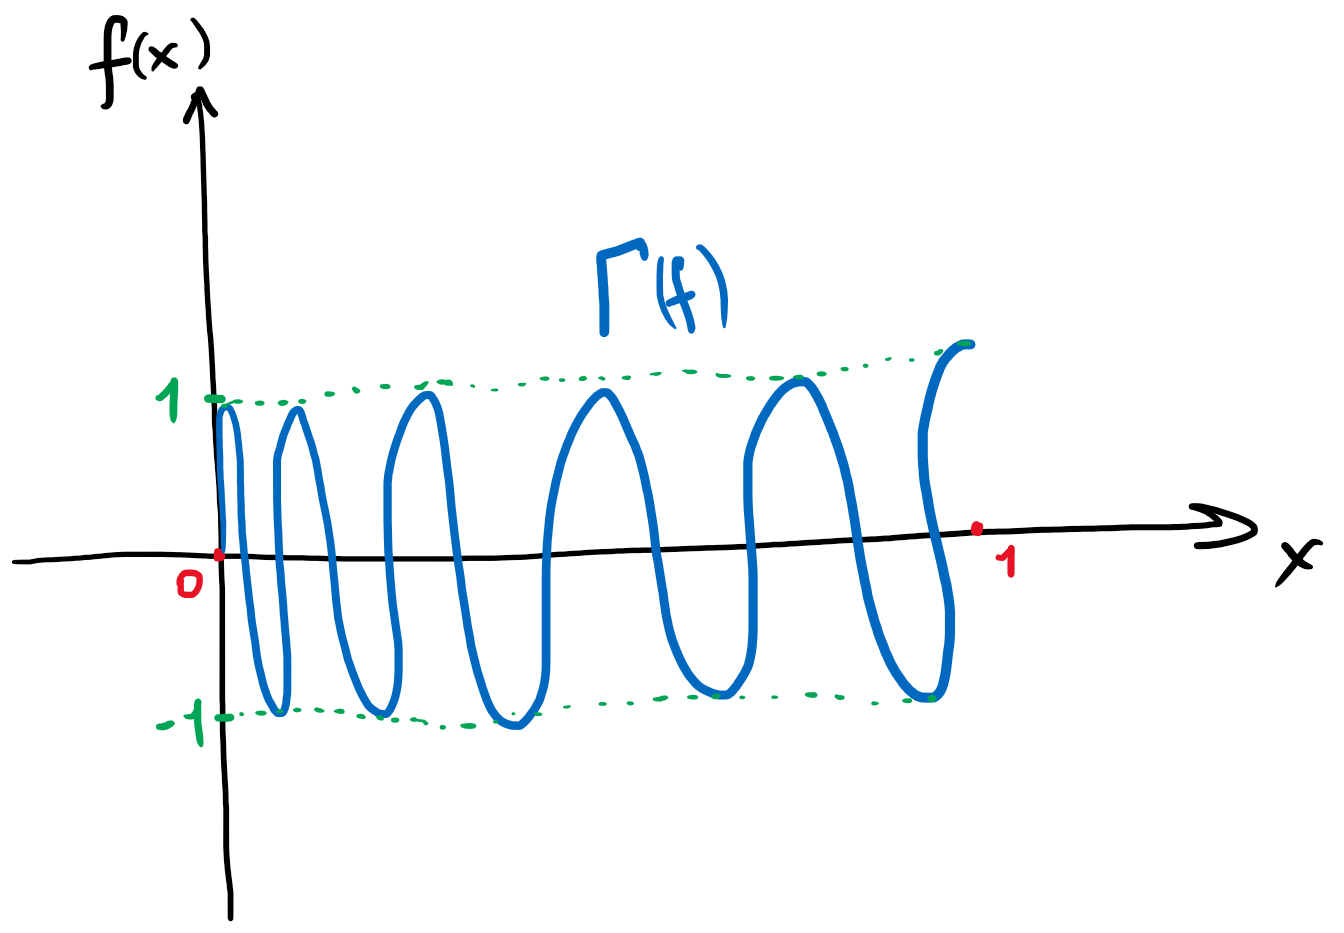
\includegraphics[width=0.5\textwidth,keepaspectratio]{img32}
\end{figure}

Sia $ S = \Gamma(f) \cup I $ dove

\begin{equation}
	I = \{ (x,y) \in \R^{2} \mid x=0 \wedge y \in (-1,1) \}
\end{equation}

Consideriamo dunque $ S \subset \R^{2} $ con la topologia indotta da $ \R^{2} $ e verifichiamo se $ S $ sia una sottovarietà di $ \R^{2} $.\\
L'insieme $ S $ con la struttura topologica indotta da $ \R^{2} $ non è una sottovarietà di $ \R^{2} $ in quanto non è nemmeno una varietà differenziabile: preso un punto $ p \in I $ e un intorno circolare $ U \ni p $, otteniamo che l'insieme $ U \cap S $ non è connesso in quanto costituito da infiniti segmenti disgiunti e dunque non può essere localmente euclideo poiché $ \R^{n} $ è connesso, quindi $ S $ non è una varietà.\\
Naturalmente, non è nemmeno possibile trovare una carta adattata che renda $ S $ una sottovarietà.

\paragraph{2. Cuspide cubica}

Sia l'insieme

\begin{equation}
	S = \{ (x,y) \in \R^{2} \mid y^{2}=x^{3} \}
\end{equation}

\begin{figure}[H]
	\centering
	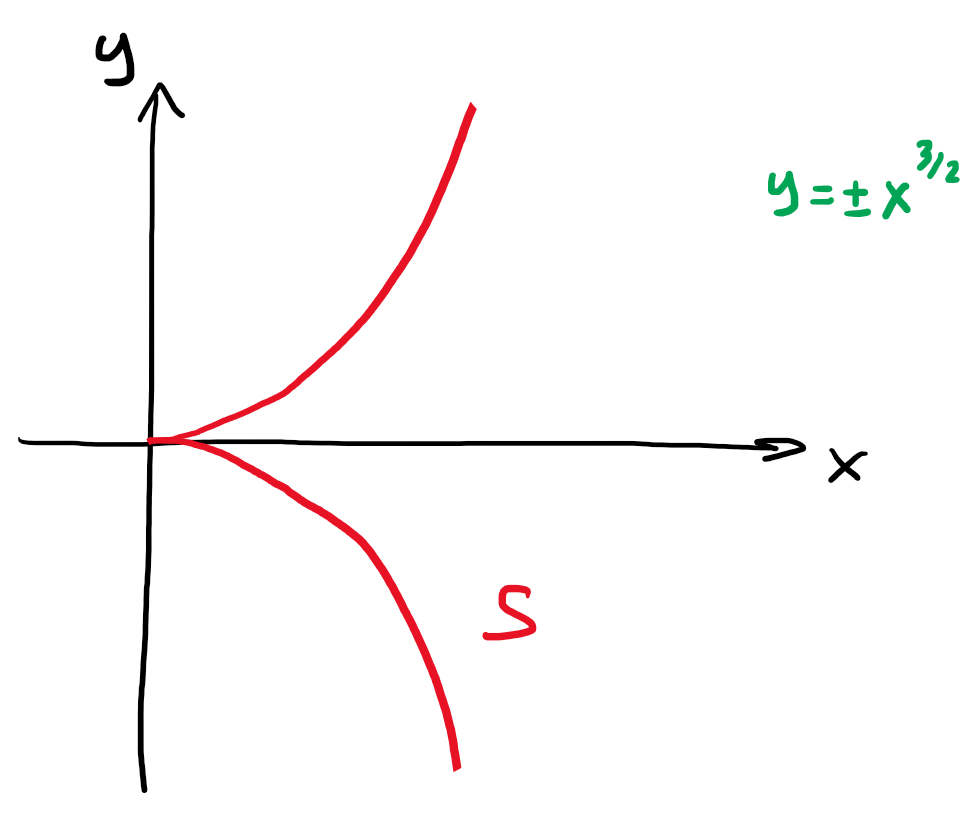
\includegraphics[width=0.3\textwidth,keepaspectratio]{img33}
\end{figure}

L'insieme $ S $ con la struttura topologica indotta da $ \R^{2} $ non è una sottovarietà di $ \R^{2} $ ma è una varietà di dimensione unitaria (curva) rispetto alla struttura topologica indotta da $ \R^{2} $. Possiamo definire l'applicazione che proietta i punti di $ S $ lungo l'asse verticale, i.e.

\begin{align}
	\begin{split}
		\psi : S &\to \R\\
		(x,y) &\mapsto y
	\end{split}
\end{align}

la quale individua un'unica carta per $ S $ che definisce una struttura differenziabile (è compatibile con sé stessa).\\\\
%
Mostriamo ora che $ S $ non è una sottovarietà di $ \R^{2} $ attraverso il fatto che l'inclusione $ i : S \to \R^{2} $ non è un'immersione nel punto 0 e dunque non può esserlo per $ \forall p \in S $.\\
Supponiamo per assurdo che questa inclusione sia un'immersione e sia $ (U,\phi) $ una carta di $ S $ intorno a 0 con $ \phi : U \to (a,b) \subset \R $ tale che $ \phi^{-1}(0)=(0,0) $ e $ \phi $ sia un diffeomorfismo

\begin{figure}[H]
	\centering
	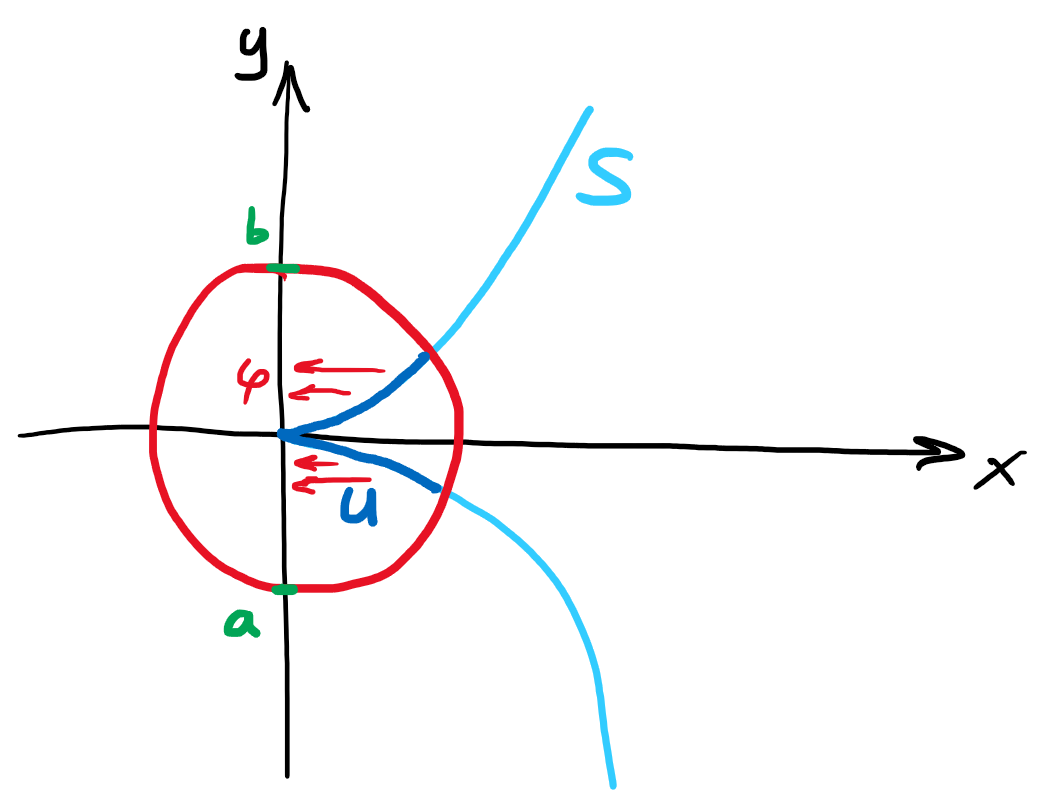
\includegraphics[width=0.4\textwidth,keepaspectratio]{img34}
\end{figure}

Definiamo l'applicazione liscia

\begin{equation}
	h = i \circ \phi^{-1} : (a,b) \to \R^{2}
\end{equation}

la quale è un'immersione in quanto composizione di un isomorfismo e di un'immersione\footnote{%
	La composizione di immersioni è ancora un'immersione: questo fatto deriva dal fatto che la composizione di funzioni iniettive (in questo caso differenziali) è ancora una funzione iniettiva.%
}, tale che $ h(0)=(0,0) $. Scrivendo $ h(t) = (h_{1}(t),h_{2}(t)) $, sappiamo che

\begin{equation}
	\begin{cases}
		h_{1}(0) = 0\\
		h_{2}(0) = 0\\
		h_{1}(t) \geqslant 0\\
		h_{1}(t) = (h_{2}(t))^{\sfrac{2}{3}}
	\end{cases}
\end{equation}

Deriviamo l'ultima equazione rispetto a $ t $

\begin{equation}
	\dot{h}_{1}(t) = \dfrac{2}{3} \, (h_{2}(t))^{-\sfrac{1}{3}} \, \dot{h}_{2}(t)
\end{equation}

per $ t \to 0 $ abbiamo che

\begin{align}
	\begin{split}
		\dot{h}_{1}(0) &= \dfrac{2}{3} \, (h_{2}(0))^{-\sfrac{1}{3}} \, \dot{h}_{2}(0)\\
		&= \dfrac{2 \, \dot{h}_{2}(0)}{3 \, (h_{2}(0))^{\sfrac{1}{3}}}
	\end{split}	
\end{align}

siccome $ h_{2}(0)=0 $, otteniamo che $ \dot{h}_{2}(0) $ deve tendere a 0 per far sì che $ \dot{h}_{1}(0) $ sia finito.\\
Sappiamo inoltre che $ \dot{h}_{1}(0) \neq 0 $ perché se consideriamo la funzione $ h $ come una curva

\begin{align}
	\begin{split}
		h : (a,b) &\to \R^{2}\\
		t &\mapsto (h_{1}(t),h_{2}(t))
	\end{split}	
\end{align}

e la differenziamo

\begin{align}
	\begin{split}
		h'(0) &= h_{*0} \left( \left. \dfrac{\operatorname{d}}{\operatorname{dt}} \right|_{0} \right) \\
		&= \dot{h}_{1}(0) \left. \dfrac{\partial}{\partial x} \right|_{(0,0)} + \dot{h}_{2}(0) \left. \dfrac{\partial}{\partial y} \right|_{(0,0)}
	\end{split}
\end{align}

e se $ \dot{h}_{1}(0) = \dot{h}_{2}(0) = 0 $ allora $ h'(0) = 0 $ e quindi $ h_{*0} (\sfrac{\operatorname{d}}{\operatorname{dt}} |_{0} ) = 0 $, i.e.

\begin{align}
	\begin{split}
		h_{*0} : T_{0}((a,b)) &\to T_{(0,0)}(\R^{2})\\
		\left. \dfrac{\operatorname{d}}{\operatorname{dt}} \right|_{0} &\mapsto 0
	\end{split}
\end{align}

ma questo non è possibile in quanto $ h $ è un'immersione quindi il suo differenziale deve essere iniettivo.\\
Da questo ragionamento, sappiamo ora che $ \dot{h}_{2}(0)=0 $ e $ \dot{h}_{1}(0) \neq 0 $:

\begin{itemize}
	\item se $ \dot{h}_{1}(0) > 0 $ allora esiste un intorno di $ 0 \in (a,b) $ dove $ h_{1} $ è strettamente crescente, dunque esiste un punto $ t_{0}<0 $ tale che $ h_{1}(t_{0}) < h_{1}(0) $ il quale è assurdo perché $ h_{1}(0) = 0 $ e $ h_{1}(t) \geqslant 0 $, i.e. non esiste un $ t_{0} $ tale che $ h_{1}(t_{0}) < 0 $;
	
	\item se $ \dot{h}_{1}(0) < 0 $ allora esiste un intorno di $ 0 \in (a,b) $ dove $ h_{1} $ è strettamente decrescente, dunque esiste un punto $ t_{0}>0 $ tale che $ h_{1}(0) > h_{1}(t_{0}) $ il quale è assurdo perché $ h_{1}(0) = 0 $ e $ h_{1}(t) \geqslant 0 $, i.e. non esiste un $ t_{0} $ tale che $ h_{1}(t_{0}) < 0 $.
\end{itemize}

Questo assurdo invalida la supposizione che l'inclusione $ i : S \to \R^{2} $ sia un'immersione e dunque, per la proposizione, che $ S $ sia una sottovarietà di $ \R^{2} $.\\
La dimensione di $ S $ non può che essere unitaria in quanto, essendo un sottoinsieme di $ \R^{2} $ ci potrebbero essere solo altri due casi

\begin{itemize}
	\item $ \dim(S)=0 $ : l'insieme $ S $ è un insieme discreto di punti, fatto che non si verifica per la cuspide cubica, la quale è connessa e inoltre è immagine di un insieme continuo
	
	\item $ \dim(S)=2 $ : esiste un intorno dell'origine omeomorfo ad $ \R^{2} $, ma questo non è possibile perché, togliendo l'origine dall'intorno\footnote{%
		Un esempio di intorno nell'origine di $ S $ è l'insieme $ U $ definito sopra per la carta.%
	} questo diventa non connesso e quindi non omeomorfo a $ \R^{2} \setminus \{0\} $ il quale è ancora un insieme connesso.
\end{itemize}

\paragraph{3. Sfera (metodo generale per la determinazione di sottovarietà)}

Sappiamo che la sfera unitaria $ \S^{2} $ è una varietà differenziabile di dimensione 2, dimostriamo quindi che è anche una sottovarietà di $ \R^{3} $.\\
La sfera $ \S^{2} $ è definita come

\begin{equation}
	\S^{2} = \{ (x,y,z) \in \R^{3} \mid x^{2} + y^{2} + z^{2} = 1 \}
\end{equation}

L'idea alla base è quella di sfruttare la seguente applicazione liscia

\begin{align}
	\begin{split}
		f : \R^{3} &\to \R\\
		(x,y,z) &\mapsto x^{2} + y^{2} + z^{2} - 1
	\end{split}
\end{align}

in modo tale da avere la sfera come controimmagine del punto 0, i.e.

\begin{equation}
\S^{2} = f^{-1}(\{0\}) \doteq f^{-1}(0)
\end{equation}

Osserviamo che $ 0 \in \mathcal{VR}_{f} $, cioè la controimmagine di 0, i.e. la sfera, è costituita da tutti e soli punti regolari, cioè punti in cui il differenziale di $ f $ è suriettivo. In simboli

\begin{gather}
	p \in \mathcal{PR}_{f}, \, \forall p \in f^{-1}(0) = \S^{2}\nonumber\\
	\Updownarrow\\
	f_{*p} : T_{p}(\R^{3}) \to T_{0}(\R) \text{ suriettiva}\nonumber
\end{gather}

Sappiamo inoltre che queste condizioni sono equivalenti al fatto che le derivate parziali

\begin{equation}
	\dfrac{\partial f}{\partial x} (p), \, \dfrac{\partial f}{\partial y} (p), \, \dfrac{\partial f}{\partial z} (p)
\end{equation}

non si annullano contemporaneamente, in quanto per la sfera

\begin{equation}
	\begin{cases}
		\dfrac{\partial f}{\partial x} (p) = 2x(p)\\\\
		%
		\dfrac{\partial f}{\partial y} (p) = 2y(p)\\\\
		%
		\dfrac{\partial f}{\partial z} (p) = 2z(p)
	\end{cases}
\end{equation}

si annullano solo per $ p=0 $ ma $ (0,0,0) \notin \S^{2} $ quindi $ 0 \in \mathcal{VR}_{f} $.
Sia $ p \in \S^{2} $ e supponiamo che $ x(p) \neq 0 $ (i.e. la prima coordinata di $ p $ on è nulla) e sia l'applicazione liscia

\begin{align}
	\begin{split}
		g : \R^{3} &\to \R^{3}\\
		(x,y,z) &\mapsto (f(x,y,z),y,z)
	\end{split}
\end{align}

Lo jacobiano della funzione appena definita è pari a

\begin{equation}
	J(g)(p) = \begin{bmatrix} \dfrac{\partial f}{\partial x} (p) & \dfrac{\partial f}{\partial y} (p) & \dfrac{\partial f}{\partial z} (p) \\\\ 0 & 1 & 0 \\\\ 0 & 0 & 1 \end{bmatrix} = \begin{bmatrix} 2x(p) & 2y(p) & 2z(p) \\\\ 0 & 1 & 0 \\\\ 0 & 0 & 1 \end{bmatrix}
\end{equation}

il cui determinante è

\begin{align}
	\begin{split}
		\det(J(g)(p)) &= \dfrac{\partial f}{\partial x} (p)\\
		&= 2x(p) \neq 0
	\end{split}
\end{align}

Per il corollario del teorema della funzione inversa\footnote{%
	Vedi Corollario \ref{ift-cor}.%
}, esiste un intorno aperto $ U \subset \R^{3} $ di $ p $ tale che $ g_{|U} : U \to g(U) $ sia un diffeomorfismo e dunque $ (U,g_{|U}) $ è una carta di $ \R^{3} $: in questo caso, $ (U,g_{|U}) $ con $ g_{|U} = (f,y,z) $ è una carta adatta di $ \R^{3} $ intorno a $ p $ relativamente ad $ \S^{2} $. La verifica, è necessario che $ U \cap \S^{2} $ sia un'insieme dato dall'annullarsi di una coordinata:

\begin{equation}
	U \cap \S^{2} = \{ q \in U \mid f(q) = 0 \} \equiv \S^{2}
\end{equation}

A questo punto, intorno a tutti i punti $ p $ che hanno $ x(p) \neq 0 $ esiste una carta adattata. Il ragionamento è analogo per le altre due coordinate.\\
In conclusione, per definizione, $ \S^{2}$ è una sottovarietà di $\R^{3} $ con $ \dim(\S^{2})=2 $.

\subsubsection{Preimmagini e sottovarietà}

\begin{theorem}[Preimmagine di un valore regolare (caso $ M = \R $)]
	Siano $ N $ una varietà differenziabile con $ \dim(N)=n $, $ f : N \to \R $ un'applicazione liscia e $ c \in \mathcal{VR}_{f} \cap f(N) $\footnote{%
		$ q \notin f(N) \implies q \in \mathcal{VR}_{f}, \, \forall q \in N $%
	}, i.e. $ f^{-1}(c) \neq 0 $, allora $ f^{-1}(c) $ è una sottovarietà di $ N $ con $ \dim(f^{-1}(c)) = n-1 $.
\end{theorem}

\begin{proof}
	Possiamo sempre supporre che $ c = 0 \in \R $\footnote{%
		Se consideriamo $ h : N \to \R $ con $ h(x) \doteq f(x) - c $, abbiamo che $ h^{-1}(0) = f^{-1}(0) $ e $ c \in \mathcal{VR}_{f} \iff 0 \in \mathcal{VR}_{h} $, perché $ \sfrac{\partial f}{\partial x} = \sfrac{\partial h}{\partial x} $.%
	}.\\
	Sia $ p \in f^{-1}(0) $, vogliamo quindi trovare una carta adattata di $ N $ intorno a $ p $ relativamente a $ f^{-1}(0) $. Il fatto che $ 0 \in \mathcal{VR}_{f} $ implica che almeno una delle derivate parziali di $ f $
	
	\begin{equation}
		\dfrac{\partial f}{\partial x^{1}} (p), \dots, \dfrac{\partial f}{\partial x^{n}} (p)
	\end{equation}
	
	non si annulli, per qualsiasi carta $ (U,\phi) $ con $ \phi = (x^{1},\dots,x^{n}) $ intorno a $ p $.\\
	Supponiamo che non si annulli la prima derivata\footnote{%
		Nel caso in cui lo fosse, possiamo permutare le coordinate della carta ottenendo una carta identica.%
	} e consideriamo l'applicazione liscia

	\begin{align}
		\begin{split}
			g : U &\to \R^{n}\\
			q &\mapsto (f(q),x^{2}(q),\dots,x^{n}(q))
		\end{split}
	\end{align}

	Il determinante dello jacobiano di $ g $ nel punto $ p $ vale
	
	\begin{equation}
		\det(J(g)(p)) = \det ( \begin{bmatrix} \dfrac{\partial f}{\partial x^{1}} (p) & \cdots & \cdots & \dfrac{\partial f}{\partial x^{n}} (p) \\\\ 0 & 1 & \cdots & 0 \\\\ \vdots & & \ddots & \vdots \\\\ 0 & \cdots & 0 & 1 \end{bmatrix} ) = \dfrac{\partial f}{\partial x^{1}} (p) \neq 0
	\end{equation}

	dunque, dal corollario del teorema della funzione inversa, esiste un aperto $ U_{p} $ di $ U $ (quindi di $ N $) tale che $ (U_{p},g_{|U_{p}}) $ è una carta di $ N $ intorno a $ p $. Prendendo l'intersezione
	
	\begin{equation}
		U_{p} \cap f^{-1}(0) = \{ q \in U_{p} \mid f(q)=0 \} \equiv f^{-1}(0)
	\end{equation}

	otteniamo che $ (U_{p},g_{|U_{p}}) $ è una carta adattata e quindi, siccome il punto $ p \in f^{-1}(0) $ è arbitrario, ogni punto di $ f^{-1}(0) $ ammette una carta adattata: questo dimostra che $ f^{-1}(0) $ è una sottovarietà di $ N $ con $ \dim(f^{-1}(0)) = n-1 $, in quanto solo una delle coordinate in $ U_{p} \cap f^{-1}(0) $ si annulla.
\end{proof}

\begin{definition}
	Siano $ N $ una varietà con $ \dim(N)=n $ e $ S $ una sottovarietà di $ N $ con $ \dim(S)=k \leqslant n $. La \textit{codimensione} di $ S $ in $ N $ è definita come
	
	\begin{equation}
		\operatorname{cod}_{N}(S) = n-k
	\end{equation}

	e rappresenta il numero di variabili che si annullano in una carta adattata di $ N $ relativamente ad $ S $.
\end{definition}

\begin{theorem}[Preimmagine di un valore regolare]
	Siano due varietà differenziabili $ N $ e $ M $ rispettivamente con $ \dim(N)=n $ e $ \dim(M)=m $, $ F : N \to M $ un'applicazione liscia tra varietà e $ c \in \mathcal{VR}_{f} \cap F(N) $, i.e. $ F^{-1}(c) \neq \{\} $, allora $ F^{-1}(c) $ è una sottovarietà di $ N $ con $ \dim(F^{-1}(c)) = n-m $ o equivalentemente $ \operatorname{cod}_{N}(F^{-1}(c)) = m $.\\
	Inoltre $ T_{p}(F^{-1}(c)) = \ker(F_{*p}) $ per $ \forall p \in F^{-1}(c) $, i.e. lo spazio tangente coincide con l'insieme dei vettori di $ T_{p}(N) $ che si annullano tramite il differenziale.
\end{theorem}

\begin{proof}
	Fissiamo un punto $ p \in F^{-1}(c) $ e scegliamo due carte $ (U,\phi) \in N $ intorno a $ p $ con $ \phi = (x^{1},\dots,x^{n}) $ e $ (V,\psi) \in M $ intorno a $ c $ con $ \psi = (y^{1},\dots,y^{m}) $ tale che $ \psi(c)=0 \in \R^{m} $ e $ F(U) \subseteq V $+ (in quanto $ F $ è continua).
	
	\begin{figure}[H]
		\centering
		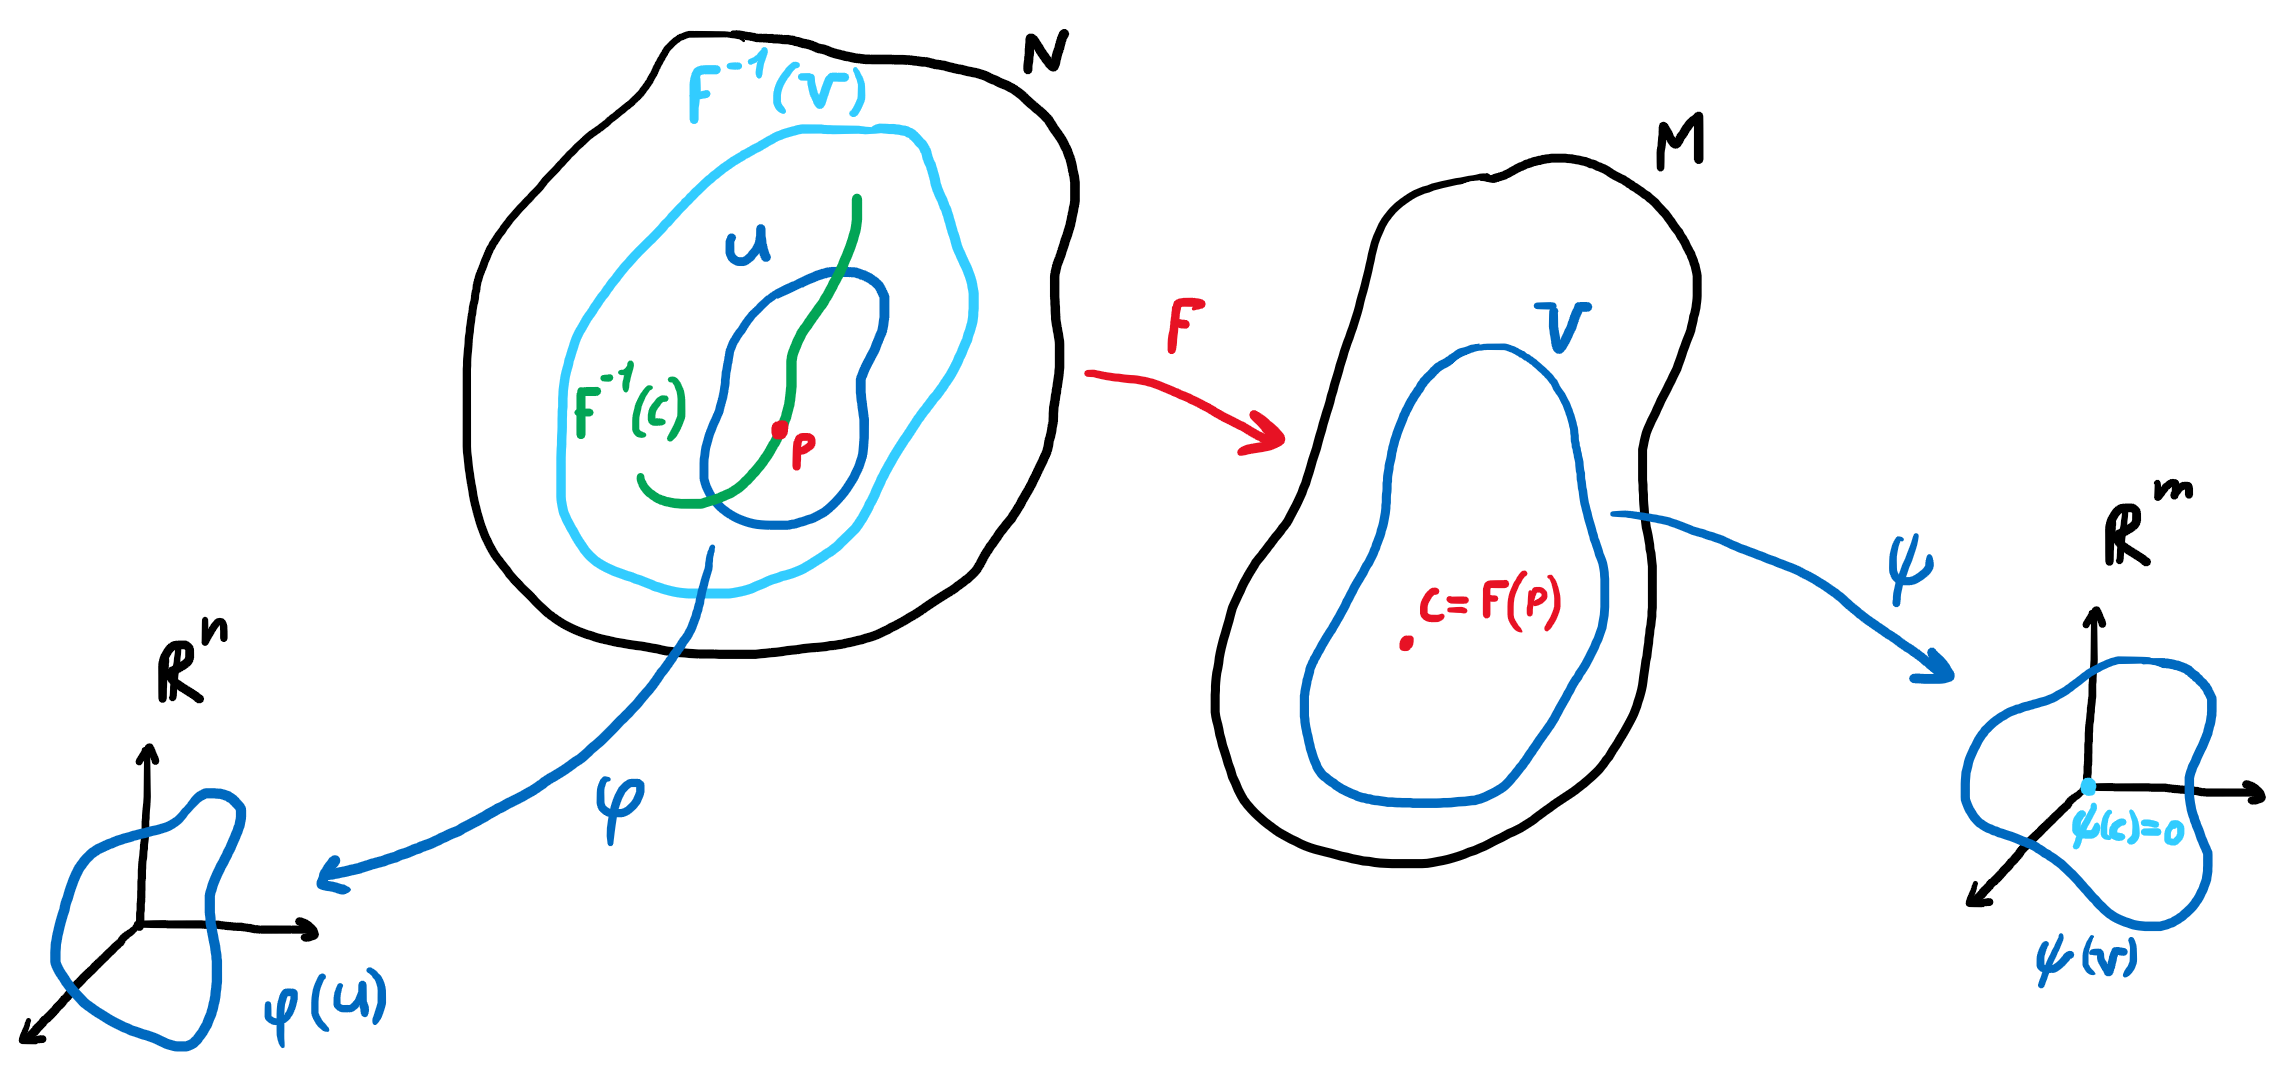
\includegraphics[width=0.7\textwidth,keepaspectratio]{img35}
	\end{figure}

	Localmente possiamo scrivere l'applicazione $ F $ come
	
	\begin{equation}
		\psi \circ F \circ \phi^{-1} : \phi(U) \to \psi(V)
	\end{equation}

	dove $ \phi(U) \subset \R^{n} $ e $ \psi(V) \subset \R^{m} $.\\
	Siccome $ c \in \mathcal{VR}_{f} $, il differenziale $ F_{*p} : T_{p}(N) \to T_{F(p)}(M) $ è suriettiva o equivalentemente $ p \in \mathcal{PR}_{F} $ o ancora $ F $ è una sommersione in $ p $. Da questo sappiamo anche che $ \rank(F(p)) = m \leqslant n $ per cui, localmente, è il rango dello jacobiano
	
	\begin{equation}
		\rank(J(F)(p)) = \rank \left( \left[ \dfrac{\partial F^{i}}{\partial x^{j}} (p) \right] \right) = m
	\end{equation}

	dove $ F^{i} = y^{i} \circ F = r^{i} \circ \psi \circ F $, e quindi esiste un minore di ordine $ m $ il quale determinante è diverso da zero: possiamo sempre supporre che il minore in questione sia quello formato dalle prime $ m $ righe e $ m $ colonne, in quanto la permutazione di coordinate all'interno delle carte le lascia invariate, i.e.
	
	\begin{equation}
		\det( \left[ \dfrac{\partial F^{i}}{\partial x^{j}} (p) \right] ) \neq 0
	\end{equation}

	con $ i,j=1,\dots,m $.\\
	Definisco l'applicazione liscia
	
	\begin{align}
		\begin{split}
			g : U &\to \R^{n}\\
			q &\mapsto (F^{1}(q),\dots,F^{m}(q),x^{m+1}(q),\dots,x^{n}(q))
		\end{split}
	\end{align}

	dove abbiamo sostituito le prime $ m $ coordinate con l'immagine di $ q $ tramite $ (F^{1},\dots,F^{m}) $, il cui jacobiano è
	
	\begin{align}
		\begin{split}
			J(g)(p) &= %
			\begin{bmatrix}
				\dfrac{\partial F^{1}}{\partial x^{1}} (p) & \dfrac{\partial F^{1}}{\partial x^{1}} (p) & \cdots & \dfrac{\partial F^{1}}{\partial x^{m}} (p) & \dfrac{\partial F^{1}}{\partial x^{m+1}} (p) & \dfrac{\partial F^{2}}{\partial x^{m+2}} (p) & \cdots & \dfrac{\partial F^{1}}{\partial x^{n}} (p) \\\\
				%
				\dfrac{\partial F^{2}}{\partial x^{1}} (p) & \dfrac{\partial F^{2}}{\partial x^{1}} (p) & \cdots & \dfrac{\partial F^{2}}{\partial x^{m}} (p) & \dfrac{\partial F^{2}}{\partial x^{m+1}} (p) & \dfrac{\partial F^{2}}{\partial x^{m+2}} (p) & \cdots & \dfrac{\partial F^{2}}{\partial x^{n}} (p) \\\\
				%
				\vdots & \vdots & \ddots & \vdots & \vdots & \vdots & \ddots & \vdots \\\\
				%
				\dfrac{\partial F^{m}}{\partial x^{1}} (p) & \dfrac{\partial F^{m}}{\partial x^{1}} (p) & \cdots & \dfrac{\partial F^{m}}{\partial x^{m}} (p) & \dfrac{\partial F^{m}}{\partial x^{m+1}} (p) & \dfrac{\partial F^{2}}{\partial x^{m+2}} (p) & \cdots & \dfrac{\partial F^{m}}{\partial x^{n}} (p) \\\\
				%
				0 & 0 & \cdots & 0 & 1 & 0 & \cdots & 0 \\\\
				%
				0 & 0 & \cdots & 0 & 0 & 1 & \cdots & 0 \\\\
				%
				\vdots & \vdots & \ddots & \vdots & \vdots & \vdots & \ddots & \vdots \\\\
				%
				0 & 0 & \cdots & 0 & 0 & 0 & \cdots & 1
			\end{bmatrix}\\\\%
			&= %
			\begin{bmatrix}
				J(F)(p) & \left[ \dfrac{\partial F^{k}}{\partial x^{h}} (p) \right] \\\\
				0 & \mathbbm{1}
			\end{bmatrix}
		\end{split}
	\end{align}

	Essendo una matrice a blocchi, il determinante di questa matrice è ottenuto dai determinanti dei blocchi, i.e.
	
	\begin{align}
		\begin{split}
			\det(J(g)(p)) &= \det \left( \begin{bmatrix} J(F)(p) & \left[ \dfrac{\partial F^{k}}{\partial x^{h}} (p) \right] \\\\ 0 & \mathbbm{1} \end{bmatrix} \right)\\\\
			&= \begin{bmatrix} \det(J(F)(p)) & \det( \left[ \dfrac{\partial F^{k}}{\partial x^{h}} (p) \right] ) \\\\ \det(0) & \det(\mathbbm{1}) \end{bmatrix}\\\\
			&= \det(J(F)(p)) \neq 0
		\end{split}
	\end{align}

	con $ i,j=1,\dots,m $.\\
	Per il corollario del teorema della funzione inversa, esiste un aperto $ U_{p} \in N $ tale che $ (U_{p},g_{|U_{p}}) $ sia una carta di $ N $ intorno a $ p $. Siccome
	
	\begin{equation}
		U_{p} \cap F^{-1}(c) = \{ q \in U_{p} \mid F^{1}(q) = \dots = F^{m}(q) = 0 \} \equiv F^{-1}(c)
	\end{equation}

	quindi $ (U_{p},g_{|U_{p}}) $ è una carta adattata di $ N $ intorno a $ p $ relativamente a $ F^{-1}(c) $, ma $ p $ è un punto arbitrario, quindi esiste una carta adattata intorno ad ogni punto. Siccome si annullano $ m $ coordinate, $ F^{-1}(c) $ è una sottovarietà di $ N $ con $ \dim(F^{-1}(c)) = n-m $ o equivalentemente $ \operatorname{cod}_{N}(F^{-1}(c)) = m $.\\\\
	%
	Dobbiamo ora dimostrare che $ T_{p}(F^{-1}(c)) = \ker(F_{*p}) $ per $ \forall p \in F^{-1}(c) $: per farlo, dimostriamo le due inclusioni
	
	\begin{equation}
		\begin{cases}
			T_{p}(F^{-1}(c)) \subset \ker(F_{*p})\\
			\ker(F_{*p}) \subset T_{p}(F^{-1}(c))
		\end{cases}
	\end{equation}
	
	Per la prima, ricordiamo che il vettore tangente ad una varietà può essere descritto come il vettore velocità di una curva (liscia) che passa per il punto della varietà considerato, definita come $ \gamma : (-\varepsilon,\varepsilon) \to F^{-1}(c) $ con $ \gamma(0) = p $ e $ \gamma'(0) = X_{p} \in T_{p}(F^{-1}(c)) $. Per definizione di controimmagine e dalla definizione della curva $ \gamma $, abbiamo che
	
	\begin{equation}
		F(\gamma(t)) = (F \circ \gamma)(t) = c
	\end{equation}
	
	per $ \forall t \in (-\varepsilon,\varepsilon) $, ma allora il differenziale
	
	\begin{align}
		\begin{split}
			F_{*p}(X_{p}) &= (F \circ \gamma)'(0)\\
			&= c'(0)\\
			&= 0 \in T_{F(p)}(M)
		\end{split}
	\end{align}

	dove $ c $ è intesa come l'applicazione costante, il cui vettore tangente è il vettore nullo, dunque $ X_{p} \in \ker(F_{*p}) $ e la prima inclusione è dimostrata.\\
	Per la seconda, è sufficiente verificare che
	
	\begin{equation}
		\dim(T_{p}(F^{-1}(c))) = \dim(\ker(F_{*p}))
	\end{equation}

	in quanto, se due spazi vettoriali (uno incluso nell'altro) hanno la stessa dimensione, allora vale l'uguaglianza tra i due: sappiamo che
	
	\begin{equation}
		\dim(T_{p}(F^{-1}(c))) = \dim(F^{-1}(c)) = n-m
	\end{equation}

	e il differenziale $ F_{*p} : T_{p}(N) \to T_{F(p)}(M) $ è suriettivo in quanto $ p \in \mathcal{PR}_{F} $ dunque, tramite il teorema della dimensione in algebra lineare
	
	\begin{align}
		\begin{split}
			\dim(\ker(F_{*p})) + \dim(\Im(F_{*p})) &= \dim(T_{p}(N))\\
			\dim(\ker(F_{*p})) + \dim(T_{F(p)}(M)) &= \dim(N)\\
			\dim(\ker(F_{*p})) + \dim(M) &= n\\
			\dim(\ker(F_{*p})) + m &= n\\
			\dim(\ker(F_{*p})) &= n-m
		\end{split}		
	\end{align}

	dove $ \dim(\Im(F_{*p})) = \dim(T_{F(p)}(M)) $ proprio perché il differenziale $ F_{*p} $ è suriettivo, perciò $ T_{p}(F^{-1}(c)) = \ker(F_{*p}) $.
\end{proof}

\begin{remark}
	Il teorema della preimmagine di un valore regolare dà una condizione sufficiente affinché si possa individuare una sottovarietà, i.e. $ F^{-1}(c) $ come sottovarietà con $ c \in \mathcal{VR}_{F} $, ma è possibile che anche la preimmagine di un valore critico sia una sottovarietà.
\end{remark}

\subsubsection{\textit{Esempi}}

\paragraph{1. Preimmagine di un valore critico come sottovarietà}

Sia l'applicazione

\begin{align}
	\begin{split}
		f : \R^{2} &\to \R\\
		(x,y) &\mapsto y^{2}
	\end{split}
\end{align}

il punto $ 0 \in \R $ annulla entrambe le derivate parziali

\begin{equation}
	\dfrac{\partial f}{\partial x} ((0,0)) = \dfrac{\partial f}{\partial y} ((0,0)) = 0
\end{equation}

dunque $ 0 \in \mathcal{VC}_{f} $, nonostante ciò la sua controimmagine è una sottovarietà di $ \R^{2} $, i.e. l'asse delle x $ f^{-1}(0) = \{(x,0)\} $,.

\paragraph{2. Sfera}

La sfera unitaria è definita come

\begin{equation}
	\S^{n} = \{ (x^{1},\dots,x^{n}) \in \R^{n} \mid (x^{1})^{2} + \cdots + (x^{n+1})^{2} = 1 \} \subset \R^{n}
\end{equation}

Sia l'applicazione liscia

\begin{align}
	\begin{split}
		f : \R^{n+1} &\to \R\\
		(x^{1},\dots,x^{n}) &\mapsto (x^{1})^{2} + \cdots + (x^{n+1})^{2} - 1
	\end{split}
\end{align}

in modo tale che $ f^{-1}(0) = \S^{n} $, dove $ 0 \in \mathcal{VR}_{f} $, in quanto $ \sfrac{\partial f}{\partial x^{i}} (p) $ non si annullano tutte contemporaneamente se non nell'origine che però non è inclusa nella sfera, dunque $ \S^{n} $ è una sottovarietà di $ \R^{n+1} $ con $ \dim(\S^{n}) = n+1-1 = n $.\\
Lo spazio tangente di $ \S^{n} $, dal teorema della preimmagine, è pari a $ T_{p}(\S^{n}) = \ker(f_{*p}) $: per calcolarlo consideriamo una curva $ \gamma : (-\varepsilon,\varepsilon) \to \S^{n} $ con $ \gamma(0) = p $ e $ \gamma'(0) = X_{p} $ e il differenziale

\begin{align}
	\begin{split}
		f_{*p} : T_{p}(\R^{n+1}) &\to T_{f(p)}(\R)\\
		X_{p} &\mapsto f_{*p}(X_{p})
	\end{split}
\end{align}

siccome $ \gamma(t) = (x^{1}(t),\dots,x^{n}(t)) $, abbiamo che

\begin{align}
	\begin{split}
		f_{*p}(X_{p}) &= (f \circ \gamma)'(0)\\
		&= ((x^{1}(t))^{2} + \cdots + (x^{n+1}(t))^{2} - 1)'(0)\\
		&= \dot{((x^{1}(t))^{2} + \cdots + (x^{n+1}(t))^{2} - 1)}(0) \left. \dfrac{\operatorname{d}}{\operatorname{dt}} \right|_{f(p)}\\
		&= (2 x^{1}(t) \dot{x}^{1}(t) + \cdots + 2 x^{n+1}(t) \dot{x}^{n+1}(t))(0)\\
		&= 2 \, \gamma(0) \cdot X_{p}\\
		&= 2 \, p \cdot X_{p}
	\end{split}
\end{align}

dove nel secondo passaggio è presente una derivata (indicata dal puntino sopra l'intera parentesi) e in quanto $ X_{p} = (\dot{x}^{1}(t),\dots,\dot{x}^{n+1}(t)) $ e il punto in $ p \cdot X_{p} $ indica il prodotto scalare in $ \R^{n+1} $.\\
A questo punto, lo spazio tangente è costituito da tutti i vettori $ X_{p} $ di $ \R^{n+1} $ che sono ortogonali al punto $ p $\footnote{%
	Cioè, presa la sfera e un piano tangente ad essa in un punto, tutti i vettori complanari al piano tangente sono tangenti alla sfera in quel punto.%
}, i.e. $ p \cdot X_{p} = 0 $.

\paragraph{3.}

Sia l'insieme

\begin{equation}
	S = \{ (x,y,z) \in \R^{3} \mid x^{3} + y^{3} + z^{3} = 1 \wedge x+y+z=0 \} \subset \R^{3}
\end{equation}

vogliamo dimostrare che $ S $ sia una sottovarietà di $ \R^{3} $ di dimensione unitaria e lo facciamo cercando un'applicazione la cui controimmagine di 0 sia $ S $.\\
Sia dunque l'applicazione

\begin{align}
	\begin{split}
		F : \R^{3} &\to \R^{2}\\
		(x,y,z) &\mapsto (x^{3}+y^{3}+z^{3}-1, x+y+z)
	\end{split}
\end{align}

dove $ F^{-1}(0) = S $. Verificare che $ 0 \in \mathcal{VR}_{F} $ è equivalente a verificare che il differenziale $ F_{*p} $, tramite il suo jacobiano, abbia rango massimo 2:

\begin{equation}/
	J(F)((x,y,x)) = \begin{bmatrix} 3x^{2} & 3y^{2} & 3z^{2} \\\\ 1 & 1 & 1 \end{bmatrix} \in M_{2,3}(\R)
\end{equation}

i punti critici di $ F $ sono

\begin{equation}
	\mathcal{PC}_{F} = \{ (x,y,z) \in \R^{3} \mid x^{2}-y^{2}=0 , \, y^{2}-z^{2}=0 \}
\end{equation}

cioè quei punti che rendono unitario il rango di $ F $. A questo punto

\begin{equation}
	0 \in \mathcal{VR}_{F} \iff S \cap \mathcal{PC}_{F} = \{\}
\end{equation}

per cui bisogna risolvere il sistema

\begin{equation}
	\begin{cases}
		x^{3} + y^{3} + z^{3} = 1\\
		x+y+z=0\\
		x = \pm y\\
		y = \pm z
	\end{cases}
\end{equation}

il quale non ha soluzione\footnote{%
	Perché abbia soluzione, per le seconda equazione si deve avere che una delle tre coordinate sia nulla e le altre due siano una l'opposta dell'altra, ma questa situazione non è permessa dalla prima equazione.%
} o, equivalentemente, $ S \cap \mathcal{PC}_{F} = \{\} $.\\
Vedi Esercizio \ref{BONUS2-3}.

\paragraph{4. Grafico di funzione}

Siano l'applicazione liscia $ F : \R^{n} \to \R $ e il suo grafico

\begin{equation}
	\Gamma(F) = \{ (x^{1},\dots,x^{n},y) \in \R^{n+1} \mid y = F(x^{1},\dots,x^{n}) \} \subset \R^{n+1}
\end{equation}

Vogliamo dimostrare che $ \Gamma(F) $ è una sottovarietà di $ \R^{n+1} $ di dimensione $ n $ e per fare ciò costruiamo una carta adattata attorno ad ogni suo punto.\\
Sia l'applicazione liscia

\begin{align}
	\begin{split}
		\phi : \R^{n+1} &\to \R^{n+1}\\
		(x^{1},\dots,x^{n},y) &\mapsto (x^{1},\dots,x^{n},y - F(x^{1},\dots,x^{n}))
	\end{split}
\end{align}

la cui inversa è liscia

\begin{align}
	\begin{split}
		\phi^{-1} : \R^{n+1} &\to \R^{n+1}\\
		(a^{1},\dots,a^{n},b) &\mapsto (a^{1},\dots,a^{n},b + F(a^{1},\dots,a^{n}))
	\end{split}
\end{align}

dunque $ \phi $ è un diffeomorfismo: questo significa che $ (\R^{n+1},\phi) $ è una carta di $ \R^{n+1} $ con la struttura standard. Questa carta può anche essere pensata come carta adattata di $ \R^{n+1} $ relativamente a $ \Gamma(F) $ per $ \forall p \in \Gamma(F) $: questo è vero in quanto l'insieme

\begin{equation}
	\R^{n+1} \cap \Gamma(F) = \{ q \in \R^{n+1} \mid y - F(x^{1},\dots,x^{n}) = 0 \}
\end{equation}

rispetta la condizione per le sottovarietà e dunque la dimensione del grafico di $ F $ è $ \dim(\Gamma(F)) = n+1-1 = n $.

\paragraph{5. Sottoinsieme del proiettivo reale}

Sia l'insieme $ S \subset \mathcal{RP}^{2} $ definito come

\begin{equation}
	S = \{ [x_{0},x_{1},x_{2}] \in \mathcal{RP}^{2} \mid x_{0}^{2} - x_{1}^{2} + x_{2}^{2} = 0 \}
\end{equation}

questo insieme è ben definito perché un altro rappresentante della classe $ (y_{0},y_{1},y_{2}) \in [x_{0},x_{1},x_{2}] $ che sia proporzionale a quello della definizione per mezzo di $ \lambda \in \R \setminus 0 $, i.e. $ (y_{0},y_{1},y_{2}) = \lambda (x_{0},x_{1},x_{2}) $, rispetta ancora la condizione.\\
Prendendo le tre carte $ (U_{i},\phi_{1}) $ con $ i=0,1,2 $ di $ \mathcal{RP}^{2} $, queste sono carte adattate relativamente ad $ S $ e dunque la rendono una sottovarietà del proiettivo reale: di seguito i tre casi per le tre carte

\begin{itemize}
	\item Prendiamo la carta $ (U_{0},\phi_{0}) $ dove
	
	\begin{align}
		\begin{split}
			U_{0} = \{ [x_{0},x_{1},x_{2}] &\in \mathcal{RP}^{2} \mid x_{0} \neq 0 \}\\\\
			\phi_{0} : U_{0} &\to \R^{2}\\
			[x_{0},x_{1},x_{2}] &\mapsto (x,y) = \left( \dfrac{x_{1}}{x_{0}}, \dfrac{x_{2}}{x_{0}} \right)
		\end{split}
	\end{align}
	
	da cui otteniamo che la condizione diventa $ 1 - x^{2} + y^{2} = 0 $ e dunque
	
	\begin{equation}
		\phi_{0}(S) = \{ (x,y) \in \R^{2} \mid x^{2} - y^{2} = 1 \}
	\end{equation}

	che rappresenta i punti di un'iperbole equilatera, la quale è una sottovarietà di $ \R^{2} $ in quanto controimmagine tramite l'applicazione
	
	\begin{align}
		\begin{split}
			f : \R^{2} &\to \R\\
			(x,y) &\mapsto x^{2} - y^{2} - 1
		\end{split}
	\end{align}

	del valore regolare $ 0 \in \mathcal{VR} $\footnote{%
		Le derivate parziali $ 2x $ e $ 2y $ si annullano solamente in 0 ma $ f^{-1}(0) \neq 0 $.%
	}, i.e. $ \phi_{0}(S) = f^{-1}(0) $;
	
	\item Prendiamo la carta $ (U_{1},\phi_{1}) $ dove
	
	\begin{align}
		\begin{split}
			U_{1} = \{ [x_{0},x_{1},x_{2}] &\in \mathcal{RP}^{2} \mid x_{1} \neq 0 \}\\\\
			\phi_{1} : U_{1} &\to \R^{2}\\
			[x_{0},x_{1},x_{2}] &\mapsto (x,y) = \left( \dfrac{x_{0}}{x_{1}}, \dfrac{x_{2}}{x_{1}} \right)
		\end{split}
	\end{align}
	
	da cui otteniamo che la condizione diventa $ x^{2} - 1 + y^{2} = 0 $ e dunque
	
	\begin{equation}
		\phi_{1}(S) = \{ (x,y) \in \R^{2} \mid x^{2} + y^{2} = 1 \}
	\end{equation}
	
	che rappresenta i punti di un cerchio\footnote{%
		Dal punto di vista della geometria proiettiva non esiste distinzione tra parabola, iperbole ed ellisse.%
	}, il quale è una sottovarietà di $ \R^{2} $ in quanto controimmagine tramite l'applicazione
	
	\begin{align}
		\begin{split}
			f : \R^{2} &\to \R\\
			(x,y) &\mapsto x^{2} + y^{2} - 1
		\end{split}
	\end{align}
	
	del valore regolare $ 0 \in \mathcal{VR} $, i.e. $ \phi_{1}(S) = f^{-1}(0) $;
	
	\item Prendiamo la carta $ (U_{2},\phi_{2}) $ dove
	
	\begin{align}
		\begin{split}
			U_{2} = \{ [x_{0},x_{1},x_{2}] &\in \mathcal{RP}^{2} \mid x_{2} \neq 0 \}\\\\
			\phi_{2} : U_{2} &\to \R^{2}\\
			[x_{0},x_{1},x_{2}] &\mapsto (x,y) = \left( \dfrac{x_{0}}{x_{2}}, \dfrac{x_{1}}{x_{2}} \right)
		\end{split}
	\end{align}
	
	da cui otteniamo che la condizione diventa $ x^{2} - y^{2} + 1 = 0 $ e dunque
	
	\begin{equation}
		\phi_{1}(S) = \{ (x,y) \in \R^{2} \mid y^{2} - x^{2} = 1 \}
	\end{equation}
	
	che rappresenta i punti di un'iperbole equilatera (ruotata di $ \sfrac{\pi}{2} $ rispetto alla prima), la quale è una sottovarietà di $ \R^{2} $ in quanto controimmagine tramite l'applicazione
	
	\begin{align}
		\begin{split}
			f : \R^{2} &\to \R\\
			(x,y) &\mapsto y^{2} - x^{2} - 1
		\end{split}
	\end{align}
	
	del valore regolare $ 0 \in \mathcal{VR} $, i.e. $ \phi_{2}(S) = f^{-1}(0) $.
\end{itemize}

\paragraph{6. Gruppo delle matrici con determinante unitario}\label{SL-subvar}

Sia l'insieme

\begin{equation}
	SL_{n}(\R) = \{ A \in GL_{n}(\R) \mid \det(A) = 1 \} \subset GL_{n}(\R) \subset M_{n}(\R) = \R^{n^{2}}
\end{equation}

il quale è una varietà differenziabile di dimensione $ n^{2} $.\\
Vogliamo dimostrare che $ SL_{n}(\R) $ è una sottovarietà di $ GL_{n}(\R) $ di dimensione $ n^{2}-1 $ o equivalentemente $ \operatorname{cod}_{GL_{n}(\R)}(SL_{n}(\R)) = 1 $ e, per dimostrarlo, usiamo il teorema della preimmagine di un valore regolare.\\
Sia l'applicazione liscia

\begin{align}
	\begin{split}
		f : GL_{n}(\R) &\to \R\\
		A &\mapsto \det(A)
	\end{split}
\end{align}

siccome $ f^{-1}(1) = SL_{n}(\R) $, dobbiamo mostrare che $ 1 \in \mathcal{VR}_{f} $: siccome il codominio di $ f $ è $ \R $, un punto è critico se e solo se le derivate parziali della funzione $ f $ si annullano in quel punto. Usiamo come coordinate le componenti della matrice, i.e. $ A = (a_{ij}) $ con $ i,j=1,\dots,n $, e per scrivere il determinante lo sviluppo di Laplace

\begin{equation}
	\det(A) = \sum_{j=1}^{n} (-1)^{i+j} \, a_{ij} \, m_{ij}
\end{equation}

dove gli $ m^{ij} = \det(A_{ij}) $ sono i minori di $ A $ e le $ A_{ij} $ sono le sottomatrici ricavate da $ A $ rimuovendo la $ i $-esima riga e la $ j $-esima colonna.\\
A questo punto, calcoliamo la derivata di $ f $ rispetto alle coordinate $ a_{ij} $

\begin{equation}
	\dfrac{\partial f}{\partial a_{ij}} = (-1)^{i+j} \, m_{ij}
\end{equation}

La condizione che individua i punti critici è la seguente

\begin{align}
	\dfrac{\partial f}{\partial a_{ij}} = 0, \, \forall i,j=1,\dots,n \iff m_{ij} = 0, \, \forall i,j=1,\dots,n
\end{align}

ma

\begin{equation}
	m_{ij} = 0, \, \forall i,j=1,\dots,n \implies \det(A) = 0
\end{equation}

Siccome quindi $ 1 \notin \mathcal{VC}_{f} $ allora $ 1 \in \mathcal{VR}_{f} $, in quanto $ \mathcal{VC}_{f} \cap \mathcal{VR}_{f} = \{\} $: questo prova che $ f^{-1}(1) = SL_{n}(\R) $ è una sottovarietà di $ GL_{n}(\R) $ di dimensione $ n^{2}-1 $.\\
Dimostreremo che\footnote{%
	Vedi Sottosezione \ref{SL-sublie}.}

\begin{equation}
	T_{I}(SL_{n}(\R)) = \{ A \in M_{n}(\R) \mid \tr(A)=0 \} \subset T_{I}(GL_{n}(\R)) = M_{n}(\R)
\end{equation}

\subsubsection{Teorema del rango costante}

\begin{theorem}[Rango costante in analisi]
	Siano $ F : W \to \R^{m} $ con $ W \subset \R^{n} $ aperto e supponiamo che esista un intorno $ I_{1} $ di un punto $ p \in W $ tale che il rango dello jacobiano della funzione $ J(F) $ in $ I_{1} $ sia pari ad un valore costante $ k $, i.e.
	
	\begin{equation}
		\rank(J(F)(q)) = \rank \left[ \dfrac{\partial F^{i}}{\partial x^{j}} (q) \right] = k \leqslant \min\{n,m\}, \qquad \forall q \in I_{1}
	\end{equation}

	Allora esistono due diffeomorfismi
	
	\begin{align}
		\begin{split}
			g : I_{1} &\to \R^{n} \, \mid \, g(p)=0\\
			h : I_{2} &\to \R^{m} \, \mid \, h(F(p))=0
		\end{split}
	\end{align}
	
	dove $ I_{2} \ni F(p) $ è un intorno di $ F(p) $ in $ \R^{m} $ tale che $ F(I_{1}) \subset I_{2} $, la cui composizione con $ F $
	
	\begin{align}
		\begin{split}
			h \circ F \circ g^{-1} : \R^{n} &\to \R^{m}\\
			(r^{1},\dots,r^{n}) &\mapsto (r^{1},\dots,r^{k},0,\dots,0)
		\end{split}
	\end{align}

	è chiamata \textit{forma canonica} di $ F $, scritta solitamente nella forma
	
	\begin{equation}
		(h \circ F \circ g^{-1})(r^{1},\dots,r^{n}) = (r^{1},\dots,r^{k},0,\dots,0)
	\end{equation}

	\begin{figure}[H]
		\centering
		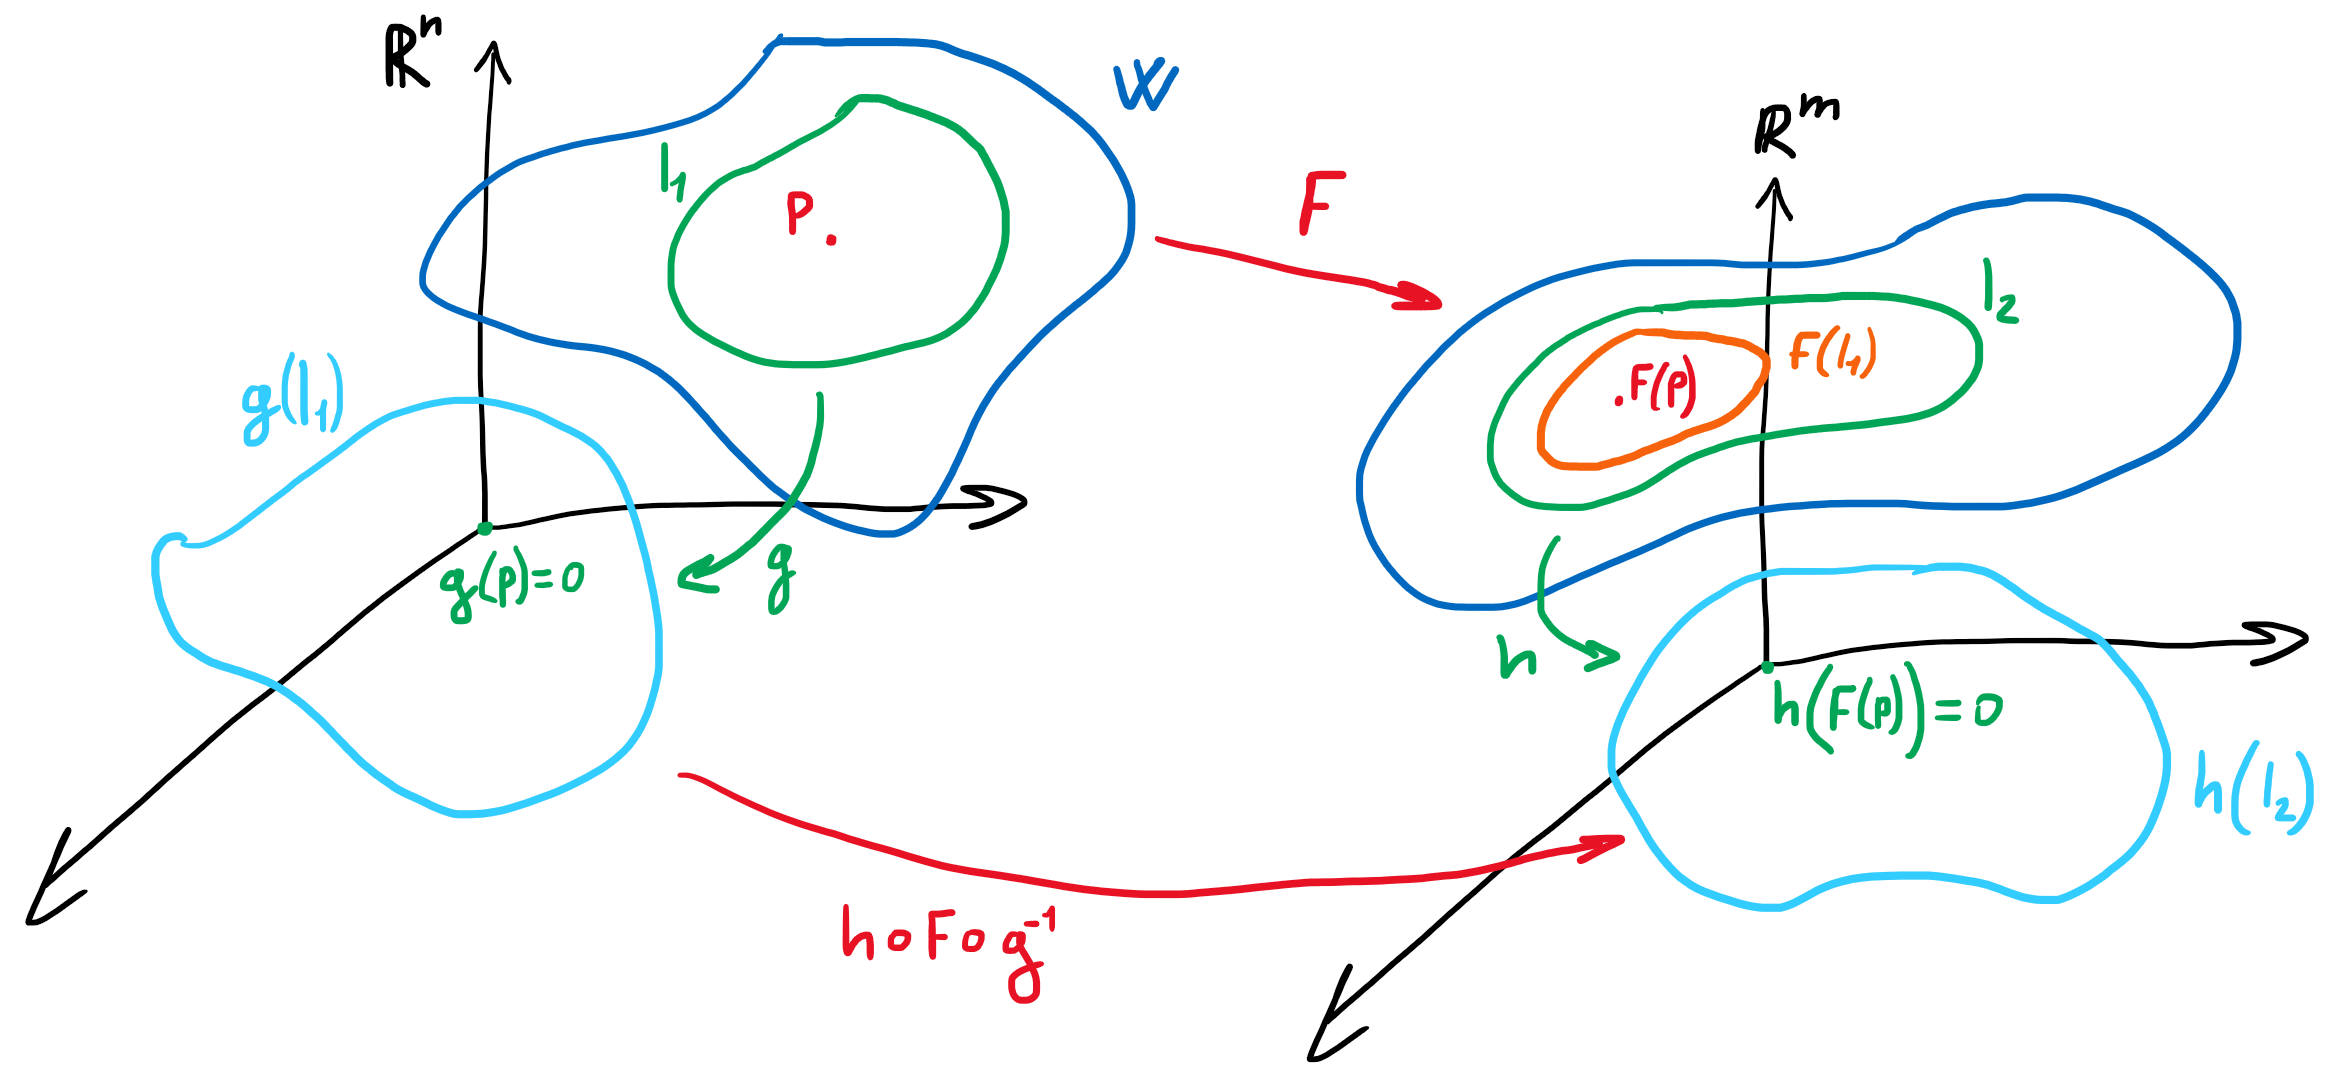
\includegraphics[width=0.7\textwidth,keepaspectratio]{img36}
	\end{figure}
\end{theorem}

\begin{theorem}[Rango costante in geometria differenziale]
	Siano $ F : N \to N $ un'applicazione liscia tra le varietà $ N $ ed $ M $ di dimensione rispettivamente $ n $ ed $ m $ e un intorno $ I $ di un punto $ p \in N $ tale che $ \rank(F(q)) = k \leqslant \min\{n,m\} $ per $ \forall q \in I $, allora esistono due carte $ (U,\phi) \in N $ centrata in $ p $ con $ \phi(p)=0 $ e $ (V,\psi) \in M $ centrata in $ F(p) $ con $ \psi(F(p))=0 $ tali che $ F(U) \subseteq V $ e la composizione tra le applicazioni delle carte ed $ F $ sia
	
	\begin{align}
		\begin{split}
			\psi \circ F \circ \phi^{-1} : \phi(U) &\to \psi(V)\\
			(r^{1},\dots,r^{n}) &\mapsto (r^{1},\dots,r^{k},0,\dots,0)
		\end{split}
	\end{align}

	dove $ \phi(U) \subset \R^{n} $ e $ \psi(V) \subset \R^{m} $, alternativamente scritta come
	
	\begin{equation}
		(\psi \circ F \circ \phi^{-1})(r^{1},\dots,r^{n}) = (r^{1},\dots,r^{k},0,\dots,0)
	\end{equation}
\end{theorem}

Questi teoremi derivano dal teorema della funzione inversa come caso particolare di quest'ultimo.

\begin{proof}
	La dimostrazione si basa sull'idea di restringere gli aperti considerati in modo tale che si possa applicare il teorema del rango costante in analisi.\\
	Consideriamo il seguente schema:
	
	\begin{figure}[H]
		\centering
		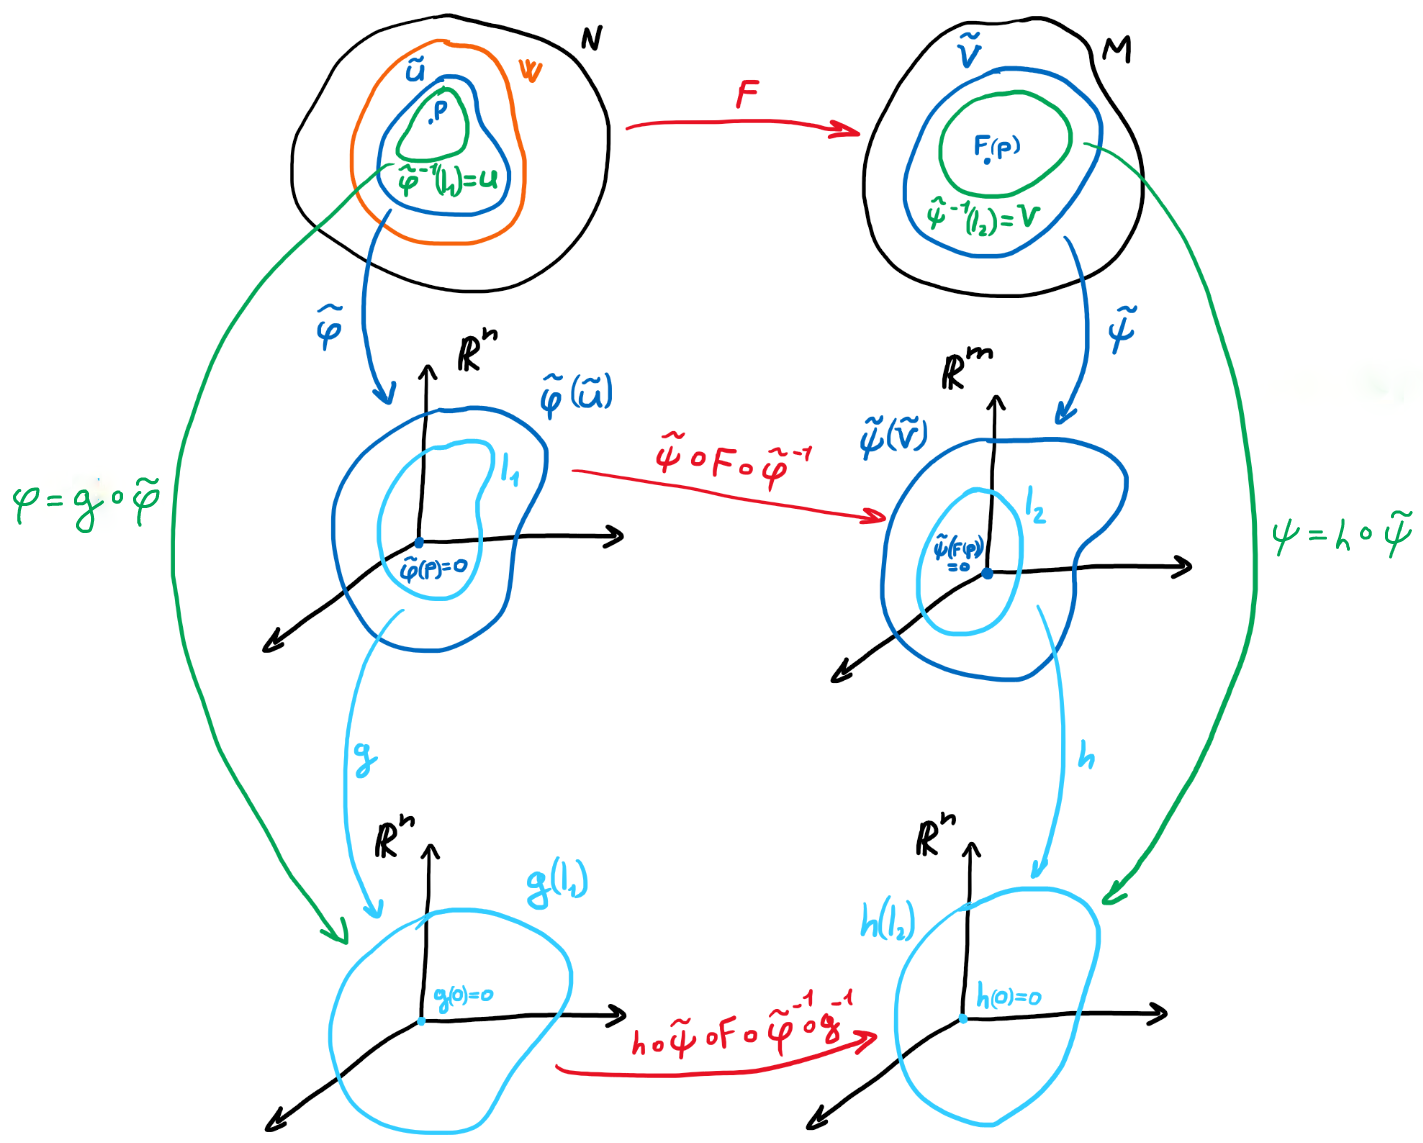
\includegraphics[width=\textwidth,keepaspectratio]{img37}
	\end{figure}

	Nell'intorno $ W \in N $ di $ p $ il rango di $ F $ è costante, i.e. $ \rank(F(q)) = k $ per $ \forall q \in W $. Consideriamo due carte arbitrarie $ (\tilde{U},\tilde{\phi}) \in N $ e $ (\tilde{V},\tilde{\psi}) \in M $ tali che $ F(\tilde{U}) \subseteq \tilde{V} $ e $ \tilde{\phi}(p) = 0 $ e $ \tilde{\psi}(F(p)) = 0 $, possiamo dunque scrivere la composizione
	
	\begin{equation}
		f = \tilde{\psi} \circ F \circ \tilde{\phi}^{-1} : \tilde{\phi}(\tilde{U}) \to \tilde{\psi}(\tilde{V})
	\end{equation}

	con $ \tilde{\phi}(\tilde{U}) \subset \R^{n} $ e $ \tilde{\psi}(\tilde{V}) \subset \R^{m} $; questa applicazione porta $ 0 \in \tilde{\phi}(\tilde{U}) $ in $ 0 \in \tilde{\psi}(\tilde{V}) $, in quanto entrambe le carte sono centrare rispettivamente in $ p $ e $ F(p) $.\\
	Essendo dominio e codominio di quest'applicazione due aperti di spazi euclidei, possiamo applicare il teorema del rango costante in analisi: sappiamo che
	
	\begin{equation}
		\rank(\tilde{\psi} \circ F \circ \tilde{\phi}^{-1})(\tilde{\phi}(q)) = k, \qquad \forall q \in \tilde{U}
	\end{equation}

	perciò esistono due aperti $ I_{1} \subset \tilde{\phi}(\tilde{U}) $ e $ I_{2} \subset \tilde{\psi}(\tilde{V}) $ entrambi centrati in nella rispettiva origine e due diffeomorfismi
	
	\begin{align}
		\begin{split}
			g : I_{1} &\to g(I_{1}) \subset \R^{n}\\
			h : I_{2} &\to h(I_{2}) \subset \R^{m}
		\end{split}
	\end{align}

	tali che $ g(0)=0 $ e $ h(0)=0 $, per i quali l'applicazione $ f $ può essere scirtta nella forma canonica
	
	\begin{align}
		\begin{split}
			h \circ f \circ g^{-1} : g(I_{1}) &\to h(I_{2})\\
			(r^{1},\dots,r^{n}) &\mapsto (r^{1},\dots,r^{k},0,\dots,0)
		\end{split}
	\end{align}

	A questo punto, possiamo considerare le carte
	
	\begin{align}
		\begin{split}
			(U,\phi) = (\tilde{\phi}(I_{1}),g \circ \tilde{\phi})\\
			(V,\psi) = (\tilde{\psi}(I_{2}),h \circ \tilde{\psi})
		\end{split}
	\end{align}

	centrate rispettivamente in $ p $ e $ F(p) $: esplicitando la composizione
	
	\begin{equation}
		h \circ f \circ g^{-1} = h \circ \tilde{\psi} \circ F \circ \tilde{\phi}^{-1} \circ g^{-1} = \psi \circ F \circ \phi^{-1}
	\end{equation}

	otteniamo dunque
	
	\begin{align}
		\begin{split}
			\psi \circ F \circ \phi^{-1} : \phi(U) &\to \psi(V)\\
			(r^{1},\dots,r^{n}) &\mapsto (r^{1},\dots,r^{k},0,\dots,0)
		\end{split}
	\end{align}
\end{proof}

\begin{theorem}[Preimmagine di un'applicazione di rango costante]
	Siano un'applicazione liscia $ F : N \to M $ tra le varietà differenziabili $ N $ e $ M $ di dimensione rispettivamente $ n $ ed $ m $ e un punto $ c \in M $ tale che $ F^{-1}(c) \neq \{\} $ e supponiamo esista un aperto $ W \subset N $ tale che $ F^{-1}(c) \subset W $ nel quale il rango di $ F $ sia costante, i.e.
	
	\begin{equation}
		\rank(F(q))=k, \qquad \forall q \in W
	\end{equation}

	Allora $ F^{-1}(c) $ è una sottovarietà di $ N $ con $ \operatorname{cod}_{N}(F^{-1}(c)) = k $ o equivalentemente $ \dim(F^{-1}(c)) = n-k $.
\end{theorem}

\begin{proof}
	Sia un punto $ p \in F^{-1}(c) $, costruiamo dunque una carta di $ N $ intorno a $ p $ relativamente a $ F^{-1}(c) $. Siano le carte
	
	\begin{itemize}
		\item $ (U,\phi) \in N $ con $ \phi = (x^{1},\dots,x^{n}) $ centrata in $ p $, i.e. $ \phi(p) = 0 \in \R^{n} $;
		
		\item $ (V,\psi) \in M $ con $ \psi = (y^{1},\dots,y^{m}) $ centrata in $ F(p) = c $, i.e. $ \psi(F(p)) = 0 \in \R^{m} $
	\end{itemize}

	tali che $ F(U) \subseteq V $ (in quanto $ F $ è continua) e
	
	\begin{align}
		\begin{split}
			\psi \circ F \circ \phi^{-1} : \phi(U) &\to \psi(V)\\
			(r^{1},\dots,r^{n}) &\mapsto (r^{1},\dots,r^{k},0,\dots,0)
		\end{split}
	\end{align}

	dove $ \phi(U) \subset \R^{n} $ e $ \psi(V) \subset \R^{m} $. Questa carte esistono perché possiamo supporre che $ U \subset W $ dove $ W $ è un intorno di $ p $ in cui il rango di $ F $ è costante con valore $ k $.\\
	Osserviamo che
	
	\begin{align}
		\begin{split}
			(\psi \circ F \circ \phi^{-1})^{-1}(0) &= \{ \phi(q) \in \phi(U) \mid r^{1}(\phi(q)) = \cdots = r^{k}(\phi(q)) = 0 \}\\
			&= \{ \phi(q) \in \phi(U) \mid x^{1}(q) = \cdots = x^{k}(q) = 0 \}
		\end{split}
	\end{align}

	siccome $ F \equiv F_{|U} $
	
	\begin{align}
		\begin{split}
			(\psi \circ F \circ \phi^{-1})^{-1}(0) &= (\psi \circ F_{|U} \circ \phi^{-1})^{-1}(0) \\
			&= (\phi \circ F_{|U}^{-1} \circ \psi^{-1})(0)\\
			&= \phi( \, F_{|U}^{-1}(\psi^{-1}(0)) \, )\\
			&= \phi( \, F_{|U}^{-1}(F(p)) \, )\\
			&= \phi( F_{|U}^{-1}(c) )\\
			&= \phi( U \cap F^{-1}(c) )
		\end{split}
	\end{align}

	dunque
	
	\begin{equation}
		\phi( U \cap F^{-1}(c) ) = \{ \phi(q) \in \phi(U) \mid x^{1}(q) = \cdots = x^{k}(q) = 0 \}
	\end{equation}

	facendo la controimmagine di questo insieme tramite $ \phi $ otteniamo
	
	\begin{equation}
		U \cap F^{-1}(c) = \{ q \in U \mid x^{1}(q) = \cdots = x^{k}(q) = 0 \}
	\end{equation}

	la quale è la condizione per cui $ (U,\phi) $ è una carta adattata di $ N $ intorno a $ p $ (arbitrario) relativamente a $ F^{-1}(c) $, rendendo perciò $ F^{-1}(c) $ una sottovarietà di $ N $ di dimensione $ n-k $.
\end{proof}

\subsubsection{\textit{Esempio}}

Dimostriamo che l'insieme delle matrici ortogonali

\begin{equation}
	O(n) = \{ A \in GL_{n}(\R) \mid A^{T} A = I_{n} \} \subset GL_{n}(\R)
\end{equation}

è una sottovarietà di $ GL_{n}(\R) $.\\
Sia l'applicazione

\begin{align}
	\begin{split}
		F : GL_{n}(\R) &\to GL_{n}(\R)\\
		A &\mapsto A^{T} A
	\end{split}
\end{align}

dunque $ O(n) = F^{-1}(I) $ dove $ I = I_{n} $.\\
Introduciamo le applicazioni traslazione a sinistra e a destra:

\begin{align}
	\begin{split}
		L_{C} : GL_{n}(\R) &\to GL_{n}(\R)\\
		A &\mapsto C A\\\\
		%
		R_{C} : GL_{n}(\R) &\to GL_{n}(\R)\\
		A &\mapsto A C
	\end{split}
\end{align}

le quali sono diffeomorfismi con inverse $ L_{C}^{-1} = L_{C^{-1}} $ e $ R_{C}^{-1} = R_{C^{-1}} $. Vale la seguente equazione

\begin{equation}
	L_{C^{T}} \circ R_{C} \circ F = F \circ R_{C}
\end{equation}

in quanto

\begin{align}
	\begin{split}
		(F \circ R_{C})(A) &= F(AC)\\
		&= (AC)^{T} (AC)\\
		&= C^{T} A^{T} A C\\
		&= C^{T} F(A) C\\
		&= (L_{C^{T}} \circ R_{C} \circ F)(A)
	\end{split}
\end{align}

Considerando $ A \in GL_{n}(\R) $, calcoliamo il differenziale dell'equazione

\begin{align}
	\begin{split}
		(L_{C^{T}} \circ R_{C} \circ F)_{*A} &= (F \circ R_{C})_{*A}\\
		L_{C^{T}_{*A^{T} A C}} \circ R_{C_{*A^{T} A}} \circ F_{*A} &= F_{*A C} \circ R_{C_{*A}}
	\end{split}
\end{align}

Siccome le traslazioni a sinistra e a destra sono diffeomorfismi, i loro differenziali sono isomorfismi, i quali non modificano il rango di applicazioni lineari, perciò

\begin{equation}
	\rank(F_{*A}) = \rank(F_{*A C})
\end{equation}

da cui, essendo $ C $ arbitrario, possiamo scrivere $ A C = B $ e

\begin{equation}
	\rank(F(A)) = \rank(F(B)), \qquad \forall A,B \in GL_{n}(\R)
\end{equation}

dunque il rango di $ F $ non dipende dalla matrice a cui si applica, i.e. il rango di $ F $ è costante in tutto $ GL_{n}(\R) $.\\
Applicando dunque il teorema, $ O(n) $ è una sottovarietà di $ GL_{n}(\R) $.

\subsection{Teoremi di immersione e sommersione locale}

Un'applicazione liscia $ F : N \to M $ tra varietà differenziabili di dimensione rispettivamente $ n $ ed $ m $ ha \textit{rango massimale} in un punto $ p \in N $ se

\begin{equation}
	\rank(F(p)) = k = \min\{n,m\}
\end{equation}

Se $ k = m \leqslant n $ allora $ F $ è una sommersione ($ F_{*p} $ suriettivo) in $ p $ invece se $ k = n \leqslant m $ allora $ F $ è un'immersione ($ F_{*p} $ iniettivo) in $ p $.

\begin{lemma}
	Sia un'applicazione liscia $ F : N \to M $ e sia $ p \in N $ tale che il rango di $ F $ in $ p $ sia massimale, allora esiste un intorno di $ p $ dove il rango di $ F $ è massimale. Equivalentemente, la condizione di \textit{rango massimale} è una \textit{condizione aperta}.
\end{lemma}

\begin{proof}
	Siano le carte $ (U,\phi) \in N $ con $ \phi = (x^{1},\dots,x^{n}) $ centrata in $ p $ e $ (V,\psi) \in M $ con $ \psi = (y^{1},\dots,y^{m}) $ centrata in $ F(p) $ tali che $ F(U) \subseteq V $ e definiamo l'insieme
	
	\begin{equation}
		W \doteq \{ q \in U \mid \rank(J(F)(q)) = \rank \left( \left[ \dfrac{\partial F^{i}}{\partial x^{j}} (q) \right] \right) = k \}
	\end{equation}

	Per ipotesi $ p \in W $ e dunque $ W \neq \{\} $. Mostriamo che $ W $ è aperto in $ U $: siccome $ U $ è aperto in $ N $, allora anche $ W $ sarà aperto in $ N $.\\
	Possiamo riscrivere $ W $ con $ \rank(J(F)(q)) \geqslant k $ perché il rango è massimale e non può essere $ >k $, dunque le condizioni sono equivalenti, i.e.
	
	\begin{equation}
		W = \{ q \in U \mid \rank(J(F)(q)) \geqslant k \}
	\end{equation}

	Il complementare di $ W $ è
	
	\begin{align}
		\begin{split}
			U \setminus W &= \{ q \in U \mid \rank(J(F)(q)) < k \}\\
			&= \{ q \in U \mid m_{1}(q) = \cdots = m_{t}(q) = 0 \}
		\end{split}
	\end{align}

	dove i $ m_{i}(q) $ sono i minori di ordine $ k $ di $ J(F)(q) $ e
	
	\begin{equation}
		t =%
			\begin{cases}
				\binom{m}{k} & k = n\\\\
				\binom{n}{k} & k = m
			\end{cases}
	\end{equation}

	Essendo i minori delle funzioni continue e $ U \setminus W $ la controimmagine di 0 (chiuso) del sistema finito di $ t $ funzioni continue
	
	\begin{equation}
		\begin{cases}
			m_{1}(q) = 0\\
			\vdots\\
			m_{t}(q) = 0
		\end{cases}
	\end{equation}

	o equivalentemente la controimmagine di 0 della funzione continua
	
	\begin{align}
		\begin{split}
			f : U &\to \R^{t}\\
			q &\mapsto (m_{1}(q),\dots,m_{t}(q))
		\end{split}
	\end{align}

	allora l'insieme $ U \setminus W = f^{-1}(0) $ è chiuso e dunque il suo complementare $ W $ è aperto.
\end{proof}

\begin{remark}
	Preso un intorno $ I $ di un punto $ p $, abbiamo che
	
	\begin{align}
		\begin{split}
			\rank(F(p)) = k \text{ massimale} &\implies \rank(F(q)) = k \text{ costante}\\
			\rank(F(p)) = k \text{ costante} &\notimplies \rank(F(p)) = k \text{ massimale}
		\end{split}
	\end{align}

	per $ \forall q \in I $.
\end{remark}

\begin{corollary}
	Sia $ F : N \to M $ un'immersione in $ p \in N $ ($ F_{*p} $ iniettivo), allora $ F $ è un'immersione in un intorno di $ p $. Analogamente, se $ F $ è una sommersione in $ p $, allora $ F $ è una sommersione in un intorno di $ p $.\\
	Questo significa che la condizione per un'applicazione di essere un'immersione o una sommersione è una condizione aperta.
\end{corollary}

\begin{proof}
	Essendo il rango dell'applicazione $ F $ massimale in $ p $ per un'immersione (risp. sommersione), esiste un intorno di $ p $ in cui il rango è costantemente uguale al massimo, dunque l'applicazione continua ad essere un'immersione (risp. sommersione) anche in questo intorno.
\end{proof}

Combinando questo corollario con il teorema del rango costante si ottengono i teoremi di immersione e sommersione locale.

\begin{theorem}[Immersione locale]\label{loc-imm}
	Sia $ F : N \to M $ ($ n \leqslant m $) un'immersione in $ p \in N $, allora esistono due carte $ (U,\phi) \in N $ con $ \phi = (x^{1},\dots,x^{n}) $ e $ \phi(p)=0 $ e $ (V,\psi) \in M $ con $ \psi = (y^{1},\dots,y^{m}) $ e $ \psi(F(p))=0 $ tali che $ F(U) \subseteq V $ e la funzione può essere scritta come \textit{immersione canonica} (inclusione)
	
	\begin{align}
		\begin{split}
			\psi \circ F \circ \phi^{-1} : \phi(U) &\to \psi(V)\\
			(r^{1},\dots,r^{n}) &\mapsto (r^{1},\dots,r^{n},0,\dots,0)
		\end{split}
	\end{align}

	dove nell'immagine ci sono $ m-n $ zeri.
\end{theorem}

\begin{theorem}[Sommersione locale]\label{loc-sub}
	Sia $ F : N \to M $ ($ n \geqslant m $) una sommersione in $ p \in N $, allora esistono due carte $ (U,\phi) \in N $ con $ \phi = (x^{1},\dots,x^{n}) $ e $ \phi(p)=0 $ e $ (V,\psi) \in M $ con $ \psi = (y^{1},\dots,y^{m}) $ e $ \psi(F(p))=0 $ tali che $ F(U) \subseteq V $ e la funzione può essere scritta come \textit{sommersione canonica} (proiezione)
	
	\begin{align}
		\begin{split}
			\psi \circ F \circ \phi^{-1} : \phi(U) &\to \psi(V)\\
			(r^{1},\dots,r^{n}) &\mapsto (r^{1},\dots,r^{m})
		\end{split}
	\end{align}
	
	dove nell'immagine ci sono le prime $ m $ coordinate del punto del dominio.
\end{theorem}

\begin{corollary}[1]\label{th-somm-loc-cor}
	Sia $ F : N \to M $ una sommersione, allora $ F $ è un'applicazione aperta.
\end{corollary}

\begin{proof}
	La sommersione è localmente aperta in quanto la sommersione canonica è un'applicazione aperta, ma un'applicazione localmente aperta è anche aperta. Infatti, se $ U \subset N $ è aperto e $ F $ è localmente aperta, allora
	
	\begin{equation}
		\forall p \in U, \, \E U_{p} \text{ intorno} \mid F_{|U_{p}} \text{ aperta}
	\end{equation}

	ma $ U $ si può scrivere come
	
	\begin{equation}
		U = \bigcup_{p \in U} U_{p}
	\end{equation}

	e applicando $ F $ si ottiene
	
	\begin{align}
		F(U) = F \left( \bigcup_{p \in U} U_{p} \right) = \bigcup_{p \in U} F(U_{p})
	\end{align}

	che è aperto in quanto unione di aperti.
\end{proof}

\begin{corollary}[2]
	Sia $ F : N \to M $ una sommersione tra varietà $ N $ compatta e $ M $ connessa, allora $ F $ è suriettiva.
\end{corollary}

\begin{proof}
	Per il primo corollario, $ F $ è aperta in quanto sommersione, mentre per il lemma dell'applicazione chiusa\footnote{%
		Vedi Lemma \ref{lemma-clos-app}.%
	} $ F $ è anche chiusa. A questo punto, l'immagine di $ N $ attraverso $ F $ è sia aperta che chiusa ma è sottoinsieme di $ M $ che è compatto ($ F(N) \subseteq M $): l'unico sottoinsieme di un compatto che è sia aperto che chiuso è il compatto stesso, dunque $ F(N) = M $ e perciò $ F $ è suriettiva.
\end{proof}

\begin{corollary}[3]
	Siano $ N $ una varietà differenziabile compatta e $ F : N \to \R^{m} $ un'applicazione liscia, allora deve esistere almeno un punto critico, i.e. $ \mathcal{PC}_{F} \neq \{\} $.
\end{corollary}

\begin{proof}
	Se per assurdo $ \mathcal{PC}_{F} = \{\} $ allora $ N = \mathcal{PR}_{F} $ e quindi $ F $ è una sommersione: per il secondo corollario $ F(N) = \R^{m} $ ma questo è assurdo in quanto $ N $ è compatta e dunque la sua immagine è compatta mentre $ \R^{m} $ non lo è (un'applicazione suriettiva porta compatti in compatti).
\end{proof}

\begin{corollary}[4]\label{imm_sph}
	Non esiste un'immersione dalla sfera $ \S^{n} $ a $ \R^{n} $.
\end{corollary}

\begin{proof}
	Se per assurdo esistesse un'immersione $ F : \S^{n} \to \R^{n} $ allora, siccome le dimensioni di dominio e codominio sono uguali, questa sarebbe anche una sommersione, in contrasto con il terzo corollario.
\end{proof}

\begin{remark}
	L'affermazione
	
	\begin{equation}
		F : N \to M \text{ liscia} \wedge c \in \mathcal{VR}_{F} \cap F(N) \implies F^{-1}(c) \text{ sottovarietà di } N
	\end{equation}

	segue dall'affermazione
	
	\begin{gather}
		F : N \to M \text{ liscia} \wedge \rank(F(q)) = k, \, \forall q \in W \supset F^{-1}(c)\nonumber\\
		\Downarrow\\
		F^{-1}(c) \text{ sottovarietà di } N\nonumber
	\end{gather}
\end{remark}

\begin{proof}
	Consideriamo la funzione $ F : N \to M $ il punto $ c \in \mathcal{VR}_{F} \cap F(N) $ dunque un punto $ p $ della controimmagine di $ c $ apparterrà a $ p \in \mathcal{PR}_{F} \cap F^{-1}(c) $. Siccome $ p $ è un punto regolare, $ F $ è una sommersione in $ p $ ($ n \geqslant m $): essendo la condizione di sommersione in un punto una condizione aperta, esiste un intorno $ U_{p} \subset N $ di $ p $ tale che
	
	\begin{equation}
		\rank(F(q)) = m, \qquad \forall q \in U_{p}
	\end{equation}
	
	Il rango della funzione $ F $ è massimale ($ m = \dim(M) $) in quanto F è una sommersione ed è costante nell'aperto $ U_{p} $ in quanto massimale in $ p $ (la condizione di rango massimale è aperta).\\
	A questo punto, al variare di $ p $, abbiamo diversi aperti di cui consideriamo l'unione
	
	\begin{equation}
		W = \bigcup_{p \in \mathcal{PR}_{F} \cap F^{-1}(c)} U_{p}
	\end{equation}
	
	la quale contiene $ F^{-1}(c) $, i.e. $ W \supset F^{-1}(c) $.\\
	Avendo considerato l'unione di aperti in cui il rango è costante (e massimale), questo sarà ancora costante (e massimale) in tutto $ W $, i.e.
	
	\begin{equation}
		\rank(F(q)) = m, \qquad \forall q \in W
	\end{equation}

	il che implica
	
	\begin{equation}
		\rank(F(q)) = m, \qquad \forall q \in F^{-1}(c)
	\end{equation}
	
	in quanto $ F^{-1}(c) \subset W $: per il teorema della preimmagine di un'applicazione di rango costante, otteniamo dunque che $ F^{-1}(c) $ è una sottovarietà di $ N $.\\	
	Questo dimostra l'implicazione in quanto abbiamo mostrato che il teorema della preimmagine di un valore regolare segue dal teorema della preimmagine di un'applicazione di rango costante, in quanto abbiamo usato il secondo teorema per dimostrare il primo.
\end{proof}

\subsection{Immagini di applicazioni lisce}

Ci chiediamo sotto quali ipotesi l'immagine di una varietà differenziabile $ N $ attraverso un'applicazione liscia $ F : N \to M $, i.e. F(N), è una sottovarietà di $ M $.\\
Supponiamo che $ N \subset M $ sia una sottovarietà, allora l'inclusione canonica

\begin{align}
	\begin{split}
		i : N &\to M\\
		q &\mapsto q
	\end{split}
\end{align}

è un'immersione iniettiva e un \textit{embedding topologico}\footnote{%
	Un embedding topologico è un'applicazione $ f : N \to M $ che individua un omeomorfismo tra $ N $ e $ f(N) $ dove quest'ultimo ha la topologia ereditata da $ M $.%
} (la condizione di embedding topologico implica l'iniettività).\\
Da questa inclusione, possiamo definire l'\textit{embedding differenziale}\footnote{%
	L'"embedding differenziale" verrà indicato semplicemente come "embedding", altrimenti verrà esplicitato "embedding topologico" nel caso in cui saremo interessati solo agli aspetti topologici.%
} come un'applicazione liscia $ F : N \to M $ che soddisfa le seguenti due condizioni:

\begin{itemize}
	\item $ F $ è un'immersione
	
	\item $ F $ è un embedding topologico
\end{itemize}

il che implica che un embedding è iniettivo. Ad esempio, come visto sopra, l'inclusione canonica è un embedding.

\begin{theorem}\label{emb-subv}
	Sia $ F : N \to M $ un embedding differenziabile, allora $ F(N) $ è una sottovarietà di $ M $ con $ \dim(N) = \dim(F(N)) $, dove $ F(N) \stackrel{diff.}{\simeq} N $ in quanto l'embedding induce un diffeomorfismo.
\end{theorem}

\begin{proof}
	La dimostrazione sfrutta il teorema di immersione locale: essendo $ F : N \to M $ un'immersione ($ n \leqslant m $), dato $ p \in N $, esistono due carte $ (U,\phi) \in N $ con $ \phi = (x^{1},\dots,x^{n}) $ e $ \phi(p)=0 $ e $ (V,\psi) \in M $ con $ \psi = (y^{1},\dots,y^{m}) $ e $ \psi(F(p))=0 $ tali che $ F(U) \subseteq V $ e
	
	\begin{align}
		\begin{split}
			\psi \circ F \circ \phi^{-1} : \phi(U) &\to \psi(V)\\
			(r^{1},\dots,r^{n}) &\mapsto (r^{1},\dots,r^{n},0,\dots,0)
		\end{split}
	\end{align}

	dove $ \phi(U) \subset \R^{n} $, $ \psi(V) \subset \R^{m} $ e nell'immagine ci sono $ m-n $ zeri.\\
	Applicando la funzione a $ \phi(U) $ otteniamo
	
	\begin{align}
		\begin{split}
			(\psi \circ F \circ \phi^{-1})(\phi(U)) &= \{ \psi(q) \in \psi(V) \mid r^{n+1}(\psi(q)) = \cdots = r^{m}(\psi(q)) = 0 \}\\
			\psi(F(U)) &= \{ \psi(q) \in \psi(V) \mid y^{n+1}(q) = \cdots = y^{m}(q) = 0 \}\\
			F(U) &= \{ q \in V \mid y^{n+1}(q) = \cdots = y^{m}(q) = 0 \}
		\end{split}
	\end{align}

	Avremmo che $ (V,\psi) $ è una carta adattata di $ M $ intorno a $ F(p) $ relativamente a $ F(N) $ se $ F(N) \cap V = F(U) $ ma, in generale questa uguaglianza è falsa: può capitare semplicemente che $ F(U) \subsetneqq F(N) \cap V $ e questa condizione non è sufficiente perché $ V $ sia una carta adattata. Ad esempio, considerando lo schema
	
	\begin{figure}[H]
		\centering
		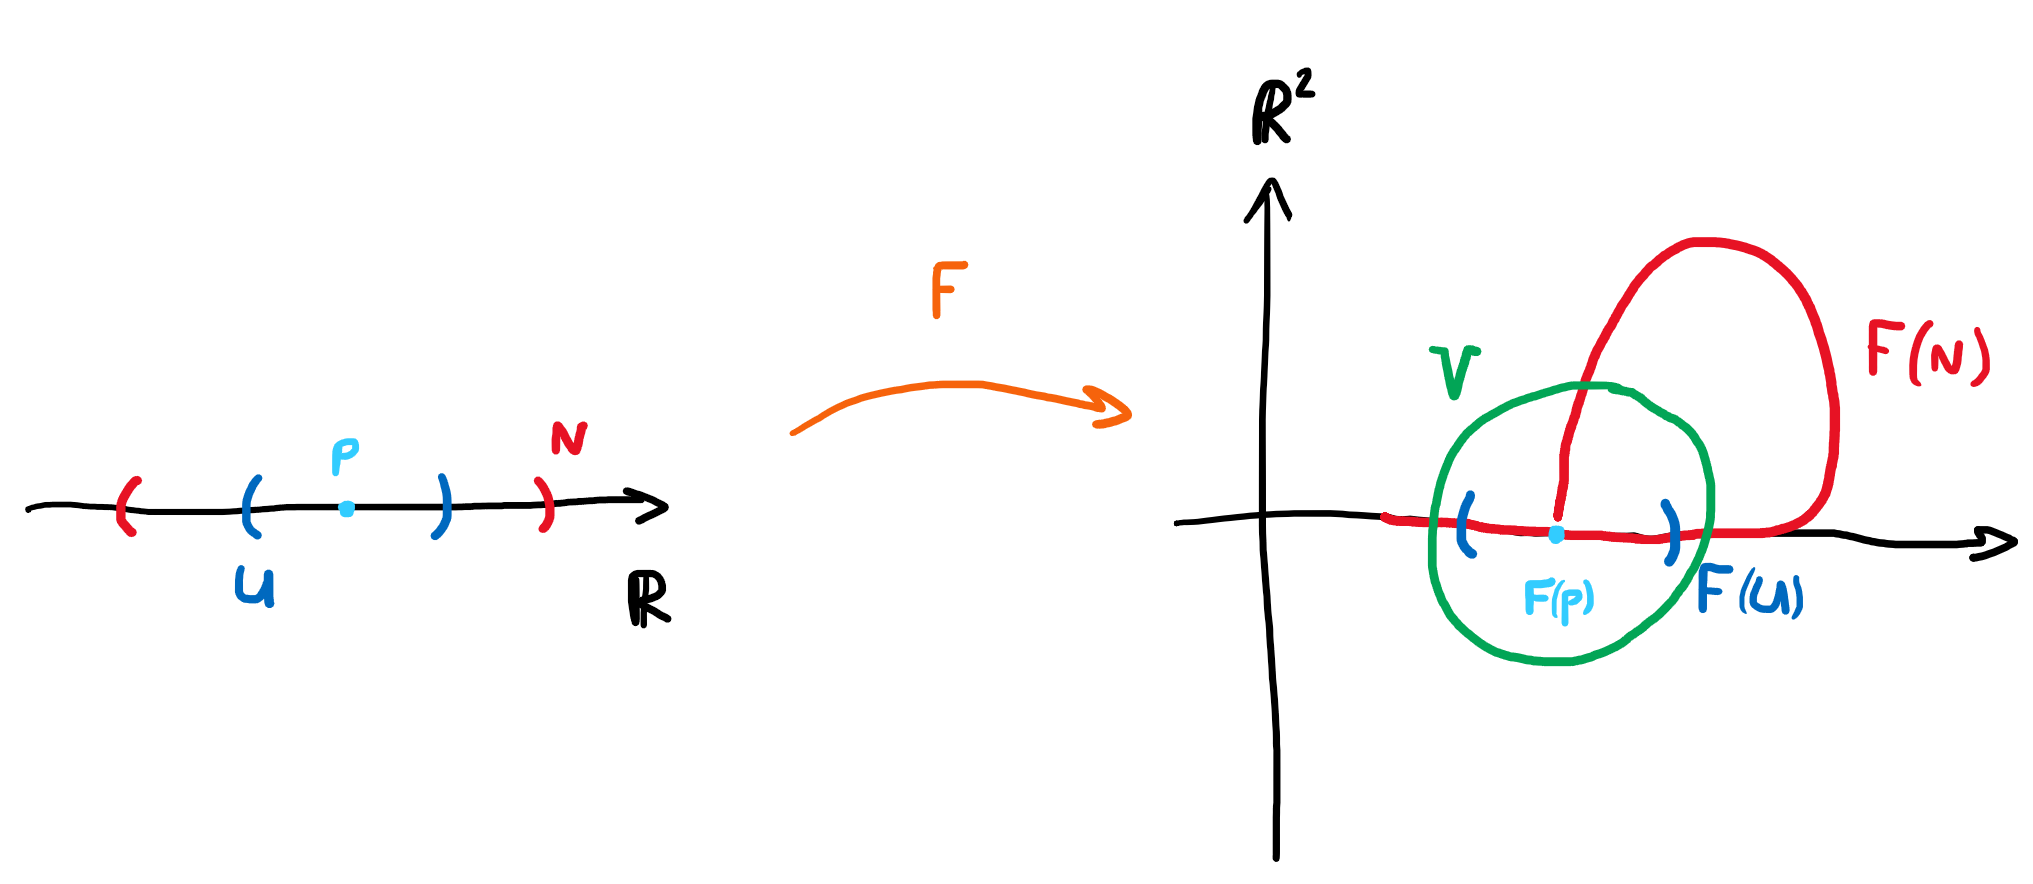
\includegraphics[width=0.7\textwidth,keepaspectratio]{img38}
	\end{figure}
	
	vediamo che, siccome un'estremità di $ F(N) $ si avvicina indefinitamente a $ F(p) $ senza toccarlo, $ F(U) \subset F(N) \cap V $ ma non è possibile trovare un aperto $ V \in \R^{2} $ tale che $ F(U) = F(N) \cap V $.\\
	Sfruttando ora il fatto che $ F $ sia anche un'embedding topologico, sappiamo che $ F(U) $ è un aperto di $ F(N) \subset M $, cioè esiste un aperto $ V' \subset M $ tale che $ F(U) = F(N) \cap V' $ (questo perché la topologia di $ F(N) $ è indotta da $ M $). Intersecando l'uguaglianza con l'aperto $ V $ della carta e chiamando $ W \doteq V \cap V' $, otteniamo
	
	\begin{equation}
		F(U) \cap V = F(N) \cap V' \cap V = F(N) \cap W
	\end{equation}

	siccome $ F(U) \subseteq V $ abbiamo che $ F(U) \cap V = F(U) $, perciò
	
	\begin{equation}
		F(N) \cap W = \{ q \in V \mid y^{n+1}(q) = \cdots = y^{m}(q) = 0 \}
	\end{equation}

	dalla definizione di $ F(U) $ sopra e dunque $ (W,\psi_{|W}) $ è una carta adattata di $ M $ intorno a $ F(p) $ relativamente a $ F(N) $ (restringendo l'aperto da $ V $ e $ W $, si ottiene la definizione per le sottovarietà). A questo punto, dato che il punto $ p $ è arbitrario, $ F(N) $ è una sottovarietà di $ M $ di dimensione $ n $.
\end{proof}

\begin{remark}[1]
	Se $ F : N \to M $ è un'immersione iniettiva, questo non implica che $ F(N) $ sia una sottovarietà di $ M $. Chiameremo dunque $ F(N) \subset M $ \textit{sottovarietà immersa}\footnote{%
		Una sottovarietà immersa non è necessariamente una sottovarietà.%
	}, la quale è diffeomorfa a $ N $ ma non ha la struttura differenziale ereditata da $ M $.
\end{remark}

\begin{remark}[2]
	Se $ F : N \to M $ è un'immersione iniettiva ed $ N $ è compatta allora $ F $ è un embedding. Per il lemma dell'applicazione chiusa\footnote{%
		Vedi Lemma \ref{lemma-clos-app}.%
	}, essendo $ F $ continua e $ M $ compatta segue che $ F : N \to F(N) $ è un omeomorfismo e quindi un embedding topologico.
\end{remark}

\begin{theorem}[Whitney]
	Se $ N $ è una varietà differenziabile di dimensione $ n $ allora esiste $ F : N \to \R^{2n} $ embedding differenziabile.\\
	Questo significa che $ F(N) $, identificabile con $ N $ tramite il diffeomorfismo $ F $, è una sottovarietà di $ \R^{2n} $.
\end{theorem}

\begin{theorem}[Whitney (forma debole)]
	Se $ N $ è una varietà differenziabile di dimensione $ n>1 $ allora esiste esiste $ F : N \to \R^{2n-1} $ immersione iniettiva.
\end{theorem}

Nel caso in cui $ n=1 $, non esiste un'immersione iniettiva tra $ N $ e $ \R $, e.g. tra $ \S^{1} $ e $ \R $\footnote{%
	Vedi Corollario \ref{imm_sph}.%
}.\\
Vedi Esercizio \ref{es2-23}.

\subsubsection{\textit{Esempi}}

\paragraph{1.}

Nell'esempio della dimostrazione del Teorema \ref{emb-subv}, $ F(N) $ non può essere una sottovarietà di $ \R^{2} $ in quanto, avendo la topologia indotta da quest'ultima, non è localmente euclideo: un qualunque intorno di $ F(p) $ non è omeomorfo ad $ \R^{n} $ in quanto il primo, togliendo il punto $ F(p) $, è formato da tre componenti connesse mentre il secondo può essere o formato da due componenti connesse (per $ \R $) o è connesso.

\paragraph{2. Cuspide cubica}

Sia l'applicazione della cuspide cubica $ y^{2} = x^{3} $ (cubica)

\begin{align}
	\begin{split}
		F : \R &\to \R^{2}\\
		t &\mapsto (x,y) = (t^{2},t^{3})
	\end{split}
\end{align}

Questa è iniettiva perché per due punti dell'immagine uguali otteniamo che

\begin{equation}
	(t_{1}^{2},t_{1}^{3}) = (t_{2}^{2},t_{2}^{3})%
	\implies%
	\begin{cases}
		t_{1}^{2} = t_{2}^{2}\\
		t_{1}^{3} = t_{2}^{3}
	\end{cases}%
	\implies%
	\begin{cases}
		t_{1} = \pm t_{2}\\
		t_{1} = t_{2}
	\end{cases}%
	\implies%
	t_{1} = t_{2}
\end{equation}

Per controllare se sia un'immersione, dobbiamo controllare che il differenziale sia iniettivo e dunque che lo jacobiano abbia rango massimale (unitario in questo caso):

\begin{equation}
	J(F) = \begin{pmatrix} 2t \\ 3t^{2} \end{pmatrix}
\end{equation}

dunque non è un'immersione perché nell'origine per $ t=0 $ il differenziale non è iniettivo.\\
Non è nemmeno un embedding in quanto la cuspide cubica non è una sottovarietà di $ \R^{2} $.\\
Con un abuso di nomenclatura, si potrebbe dire che la cuspide cubica è una "sottovarietà topologica" di $ \R^{2} $ in quanto totalmente omeomorfa (anche nell'origine) a $ \R $ e questo rende $ F $ un embedding topologico.

\paragraph{3. Cubica nodale}

Sia l'applicazione della cubica nodale $ y^{2} = x^{3} + x^{2} $ (cubica)

\begin{align}
	\begin{split}
		F : \R &\to \R^{2}\\
		t &\mapsto (x,y) = (t^{2}-1,t^{3}-t)
	\end{split}
\end{align}

\begin{figure}[H]
	\centering
	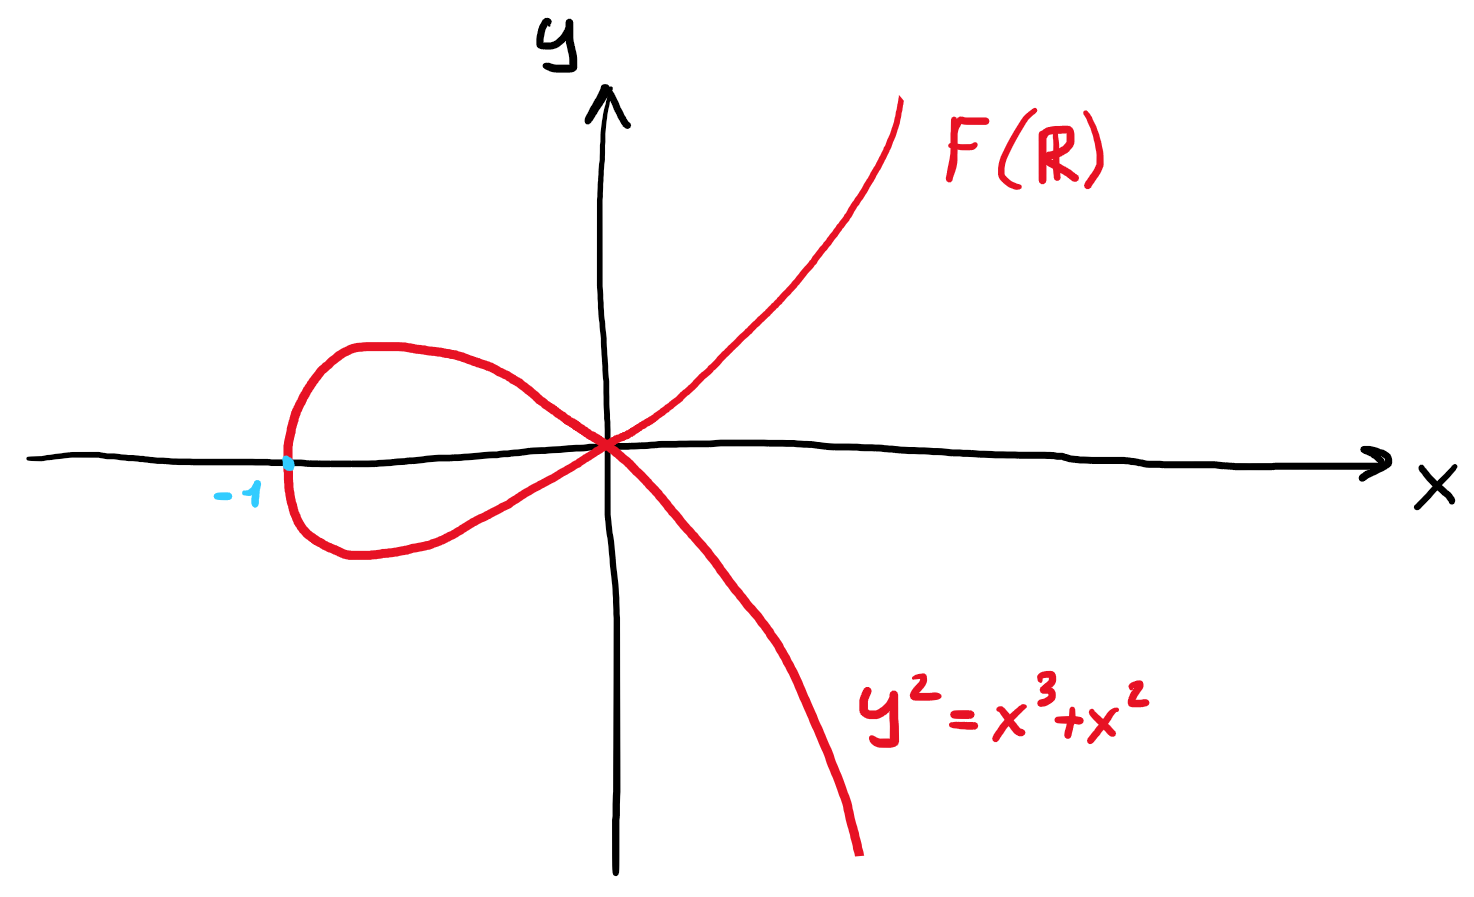
\includegraphics[width=0.5\textwidth,keepaspectratio]{img39}
\end{figure}

Questa non è iniettiva perché per esempio $ F(\pm 1) $ = 0, dunque non è nemmeno un embedding topologico.\\
Per controllare se sia un'immersione, cerchiamo un punto che annulla contemporaneamente le derivate di $ F $ rispetto a $ t $:

\begin{equation}
	\dot{F}(t) = (2t, 3 t^{2} - 1) \neq (0,0), \qquad \forall t \in \R
\end{equation}

dunque $ F $ è un'immersione.\\
Anche la cuspide cubica non è localmente euclidea nell'origine, dunque non può essere una sottovarietà di $ \R^{2} $.

\paragraph{4. Lemniscata di Bernoulli}

Sia l'applicazione della lemniscata di Bernoulli $ x^{2} = 4 y^{2} (1-y^{2}) $ (quartica)

\begin{align}
	\begin{split}
		F : (-\pi,\pi) &\to \R^{2}\\
		t &\mapsto (x,y) = (\sin(2t),\sin(t))
	\end{split}
\end{align}

\begin{figure}[H]
	\centering
	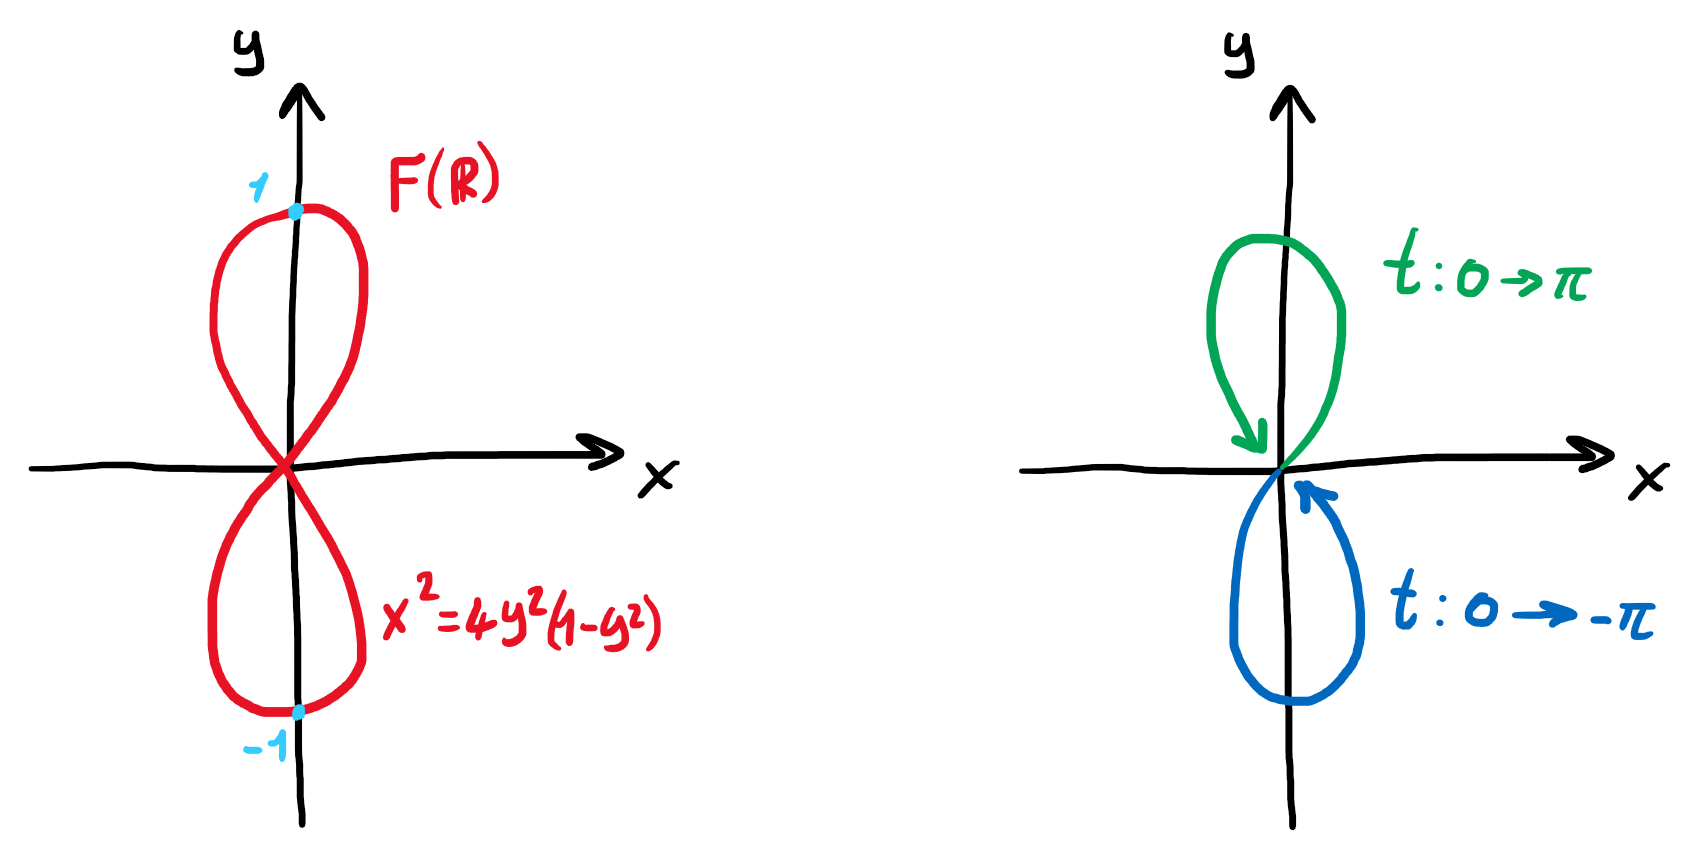
\includegraphics[width=0.7\textwidth,keepaspectratio]{img40}
\end{figure}

Questa è iniettiva perché per due punti dell'immagine uguali $ (\sin(2t_{1}),\sin(t_{1})) = (\sin(2t_{2}),\sin(2t_{2})) $ otteniamo che

\begin{equation}
	\sin(t_{1}) = \sin(t_{2}) = 0 \implies t_{1} = t_{2} = 0 \because t \in (-\pi,\pi)
\end{equation}

oppure $ \sin(t_{1}) = \sin(t_{2}) \neq 0 $ il che implica

\begin{align}
	\begin{split}
		\sin(2t_{1}) &= \sin(2t_{2})\\
		2 \sin(t_{1}) \cos(t_{1}) &= 2 \sin(t_{2}) \cos(t_{2})\\
		\cos(t_{1}) &= \cos(t_{2})
	\end{split}		
\end{align}

perciò

\begin{equation}
	\begin{cases}
		\sin(t_{1}) = \sin(t_{2})\\
		\cos(t_{1}) = \cos(t_{2})
	\end{cases}%
	\implies%
	\begin{aligned}
		t_{1} = t_{2} &+ 2 k \pi\\
		\forall k &\in \Z
	\end{aligned}
	\implies%
	t_{1} = t_{2}
\end{equation}

in quanto qualsiasi valore di $ k $ diverso da 0 esce dall'intervallo del dominio.\\
Questa applicazione è un'immersione in quanto

\begin{equation}
	\dot{F}(t) = (2 \cos(2t), \cos(t)) \neq (0,0), \qquad \forall t \in \R
\end{equation}

Nonostante sia un'immersione iniettiva, non è un embedding (né topologico né differenziabile) in quanto $ F((-\pi,\pi)) $ non è localmente euclidea nell'origine.

\paragraph{5.}

Sia l'applicazione

\begin{align}
	\begin{split}
		F : \R &\to \S^{1} \times \S^{1} = \T^{2}\\
		t &\mapsto (x,y) = (e^{2 \pi i t}, e^{2 \pi i \alpha t})
	\end{split}
\end{align}

dove $ \alpha \in \R \setminus \Q $ ($ \alpha $ irrazionale); siccome il toro $ \T^{2} $ è incluso in $ \R^{4} $, possiamo riscrivere la funzione come

\begin{align}
	\begin{split}
		F : \R &\to \R^{4}\\
		t &\mapsto (x,y) = (\cos(2 \pi t), \sin(2 \pi t), \cos(2 \pi \alpha t), \sin(2 \pi \alpha t))
	\end{split}
\end{align}

in quanto abbiamo considerato $ \S^{1} \subset \R^{2} = \C $.\\
Verifichiamo se $ F $ sia iniettiva tramite la dimostrazione dell'implicazione

\begin{equation}
	\begin{cases}
		e^{2 \pi i t_{1}} = e^{2 \pi i t_{2}}\\
		e^{2 \pi i \alpha t_{1}} = e^{2 \pi i \alpha t_{2}}
	\end{cases}%
	\implies%
	t_{1} = t_{2}
\end{equation}

Quindi possiamo scrivere

\begin{equation}
	\begin{cases}
		e^{2 \pi i t_{1}} = e^{2 \pi i t_{2}}\\
		e^{2 \pi i \alpha t_{1}} = e^{2 \pi i \alpha t_{2}}
	\end{cases}%
	\implies%
	\begin{cases}
		t_{1} - t_{2} = m & m \in \Z\\
		t_{1} - t_{2} = \alpha n & \alpha,n \in \Z
	\end{cases}%
	\implies%
	\alpha n = m%
	\implies%
	\alpha \in \Q
\end{equation}

ma questo non è possibile in quanto abbiamo posto $ \alpha \in \R \setminus \Q $, dunque l'applicazione è iniettiva.\\
Per verificare se sia un'immersione, consideriamo la derivata di $ F $ in $ \R^{4} $

\begin{equation}
	\dot{F}(t) = (- 2 \pi \sin(2 \pi t), 2 \pi \cos(2 \pi t), - 2 \pi \alpha \sin(2 \pi \alpha t), 2 \pi \alpha \cos(2 \pi \alpha t))
\end{equation}

la quale non si annulla per $ \forall t \in \R $.\\
Nonostante $ F $ sia un'immersione iniettiva, questa non è un embedding in quanto la sua immagine non è una sottovarietà di $ \R^{4} $.\\
Dimostriamo questo fatto mediante il seguente lemma


\begin{lemma}
	Chiamando $ \mathcal{D}(A) $ l'insieme dei punti di accumulazione\footnote{%
		Per un punto di accumulazione di un insieme, ogni intorno di questo punto contiene un punto dell'insieme diverso da sé stesso.%
	} di un insieme $ A $, possiamo affermare che
	
	\begin{equation}
		F(0) = (1,1) \in \mathcal{D}(F(\Z))
	\end{equation}

	Cioè qualunque intorno di $ (1,1) \in \T^{2} $ include almeno un punto di $ F(\Z) $ o equivalentemente
	
	\begin{equation}
		\forall \varepsilon > 0, \, \E k \in \Z \setminus 0 \mid \left| (e^{2 \pi i k}, e^{2 \pi i \alpha k}) - (1,1) \right| < \varepsilon
	\end{equation}
\end{lemma}

\begin{proof}
	\begin{align}
		\begin{split}
			\left| (e^{2 \pi i k}, e^{2 \pi i \alpha k}) - (1,1) \right| &< \varepsilon\\
			\left| (1, e^{2 \pi i \alpha k}) - (1,1) \right| &< \varepsilon\\
			\left| e^{2 \pi i \alpha k} - 1 \right| &< \varepsilon
		\end{split}
	\end{align}

	Sappiamo che $ \S^{1} $ è compatto quindi la successione di punti del cerchio
	
	\begin{equation}
		z_{n} = e^{2 \pi i \alpha k}, \qquad n \in \Z
	\end{equation}

	ammette una sottosuccessione convergente: possiamo supporre che (a meno di cambiare semplicemente gli indici della successione) la successione stessa converga ad un punto $ z_{n} \to z_{0} \in \S^{1} $ e ciò significa che esistono due numeri (diversi) $ n_{1},n_{2} \in \Z $ tali che si possa scrivere
	
	\begin{equation}
		\left| e^{2 \pi i \alpha n_{1}} - 1 \right| < \dfrac{\varepsilon}{2} \quad \wedge \quad \left| e^{2 \pi i \alpha n_{2}} - 1 \right| < \dfrac{\varepsilon}{2}
	\end{equation}

	ponendo dunque $ k = n_{1} - n_{2} \neq 0 $ e sfruttando la diseguaglianza triangolare
	
	\begin{align}
		\begin{split}
			\left| e^{2 \pi i \alpha k} - 1 \right| &= \left| e^{2 \pi i \alpha (n_{1} - n_{2})} - 1 \right|\\
			&= \left| e^{ -2 \pi i \alpha n_{2}} \left( e^{2 \pi i \alpha n_{1}} - e^{2 \pi i \alpha n_{2}} \right) \right|\\
			&= \left| e^{ -2 \pi i \alpha n_{2}} \right| \left| e^{2 \pi i \alpha n_{1}} - e^{2 \pi i \alpha n_{2}} \right|\\
			&= \left| e^{2 \pi i \alpha n_{1}} - e^{2 \pi i \alpha n_{2}} \right|\\
			&= \left| e^{2 \pi i \alpha n_{1}} - e^{2 \pi i \alpha n_{2}} +1 -1 \right|\\
			&\leqslant \left| e^{2 \pi i \alpha n_{1}} - 1 \right| + \left| e^{2 \pi i \alpha n_{2}} - 1 \right|\\
			&= \sfrac{\varepsilon}{2} + \sfrac{\varepsilon}{2}\\
			&= \varepsilon
		\end{split}
	\end{align}

	dunque
	
	\begin{equation}
		\left| e^{2 \pi i \alpha k} - 1 \right| < \varepsilon
	\end{equation}
\end{proof}

Supponiamo per assurdo che $ F $ sia un embedding: l'applicazione $ f : \R \to F(\R) $ con la topologia di $ F(\R) $ indotta dal toro $ \T^{2} $ è un diffeomorfismo e dunque anche un omeomorfismo. Per le proprietà degli omeomorfismi, esiste una bigezione tra i punti di accumulazione del dominio e quelli del codominio, i.e. $ \mathcal{D}(\Z) \to \mathcal{D}(F(\Z)) $, però $ \mathcal{D}(\Z) = \{\} $ in quanto i numeri interi sono isolati in $ \R $ mentre $ \mathcal{D}(F(\Z)) \ni (1,1) $. Questa contraddizione porta a dire che $ F $ non è un embedding e quindi $ F(\R) $ non è una sottovarietà di $ \T^{2} $.

\begin{remark}
	Si dimostra che $ F(\R) $ è denso in $ \T^{2} $, cioè il toro è completamente ricoperto dall'immagine della funzione o equivalentemente ogni intorno di ogni punto del toro ha al suo interno un punto dell'immagine (per dimostrare questo, viene utilizzata la teoria dei numeri).
\end{remark}

\subsubsection{Immagini di applicazioni lisce contenute in varietà}

\begin{theorem}
	Siano $ F : N \to M $ un'applicazione liscia tra varietà e $ S \subset M $ una sottovarietà di $ M $ e supponiamo che $ F(N) \subseteq S $, allora la restrizione del codominio della funzione al sottoinsieme $ S $ è ancora un'applicazione liscia, i.e. $ \tilde{F} : N \to S $ con $ \tilde{F}(q) = F(q) $ per $ \forall q \in N $.
\end{theorem}

\begin{proof}
	Sappiamo che $ \tilde{F} $ è continua in quanto $ S $ è un sottospazio topologico di $ M $.\\
	Siano $ p \in N $ un punto e due carte $ (U,\phi) \in N $ intorno a $ p $ con $ \phi = (x^{1},\dots,x^{n}) $ e $ (V,\psi) \in M $ intorno a $ F(p) $ con $ \psi = (y^{1},\dots,y^{m}) $ tali che $ F(U) \subseteq V $ e tale che $ (V,\psi) $ sia una carta adattata intorno a $ F(p) $ relativamente ad $ S $.\\
	Se $ \dim(S)=s $, possiamo scrivere la condizione per le sottovarietà
	
	\begin{equation}
		V \cap S = \{ q \in V \mid y^{s+1}(q) = \cdots = y^{m}(q) = 0 \}
	\end{equation}

	e la restrizione dell'applicazione della carta adattata
	
	\begin{align}
		\begin{split}
			\psi_{|V \cap S} = \psi_{S} : V \cap S &\to \psi(V \cap S) \subset \R^{s}\\
			q &\mapsto (y^{1}(q),\dots,y^{s}(q))
		\end{split}
	\end{align}

	Osserviamo che, dalle carte, $ F(U) \subseteq V $ e che, dalle ipotesi, $ F(N) \subseteq S $ da cui $ F(U) \subseteq S $ perciò $ F(U) \subseteq V \cap S $. Consideriamo la composizione
	
	\begin{align}
		\begin{split}
			\psi \circ F : U &\to V \subset \R^{m}\\
			q &\mapsto ( \, y^{1}(F(q)), \dots, y^{s}(F(q)), 0,\dots, 0 \, )
		\end{split}
	\end{align}

	e poi la restrizione ad $ S $
	
	\begin{align}
		\begin{split}
			\psi_{S} \circ \tilde{F} : U &\to V \cap S\\
			q &\mapsto ( \, y^{1}(F(q)), \dots, y^{s}(F(q)) \, )
		\end{split}
	\end{align}

	Siccome le $ y^{i} $, $ F $ e $ \psi_{S} $ sono tutte applicazioni lisce rispetto a $ q $, anche la composizione $ \psi_{S} \circ \tilde{F} $ sarà liscia, il che implica che la restrizione $ \tilde{F} $ è liscia.
\end{proof}

\subsubsection{\textit{Esempi}}

\paragraph{1. Lemniscata di Bernoulli}

Consideriamo le seguenti due varianti della lemniscata di Bernoulli tramite le applicazioni lisce

\begin{align}
	\begin{split}
		F : (-\pi,\pi) &\to \R^{2}\\
		t &\mapsto (\sin(2t),\sin(t))\\\\
		%
		G : (-\pi,\pi) &\to \R^{2}\\
		t &\mapsto (\sin(2t),-\sin(t))
	\end{split}
\end{align}

e chiamiamo le loro immagini $ F((-\pi,\pi)) = \mathfrak{8}_{F} $ e $ G((-\pi,\pi)) = \mathfrak{8}_{G} $, le quali sono varietà differenziabili la cui struttura è indotta rispettivamente da $ F $ o da $ G $ (bigezioni), ma non sono sottovarietà di $ \R^{2} $. Le funzioni che hanno lo stesso dominio e come codominio le immagini del dominio sono diffeomorfismi, i.e.

\begin{align}
	\begin{split}
		\tilde{F} : (-\pi,\pi) &\to \mathfrak{8}_{F}\\
		t &\mapsto (\sin(2t),\sin(t))\\\\
		%
		\tilde{G} : (-\pi,\pi) &\to \mathfrak{8}_{G}\\
		t &\mapsto (\sin(2t),-\sin(t))
	\end{split}
\end{align}

\begin{figure}[H]
	\centering
	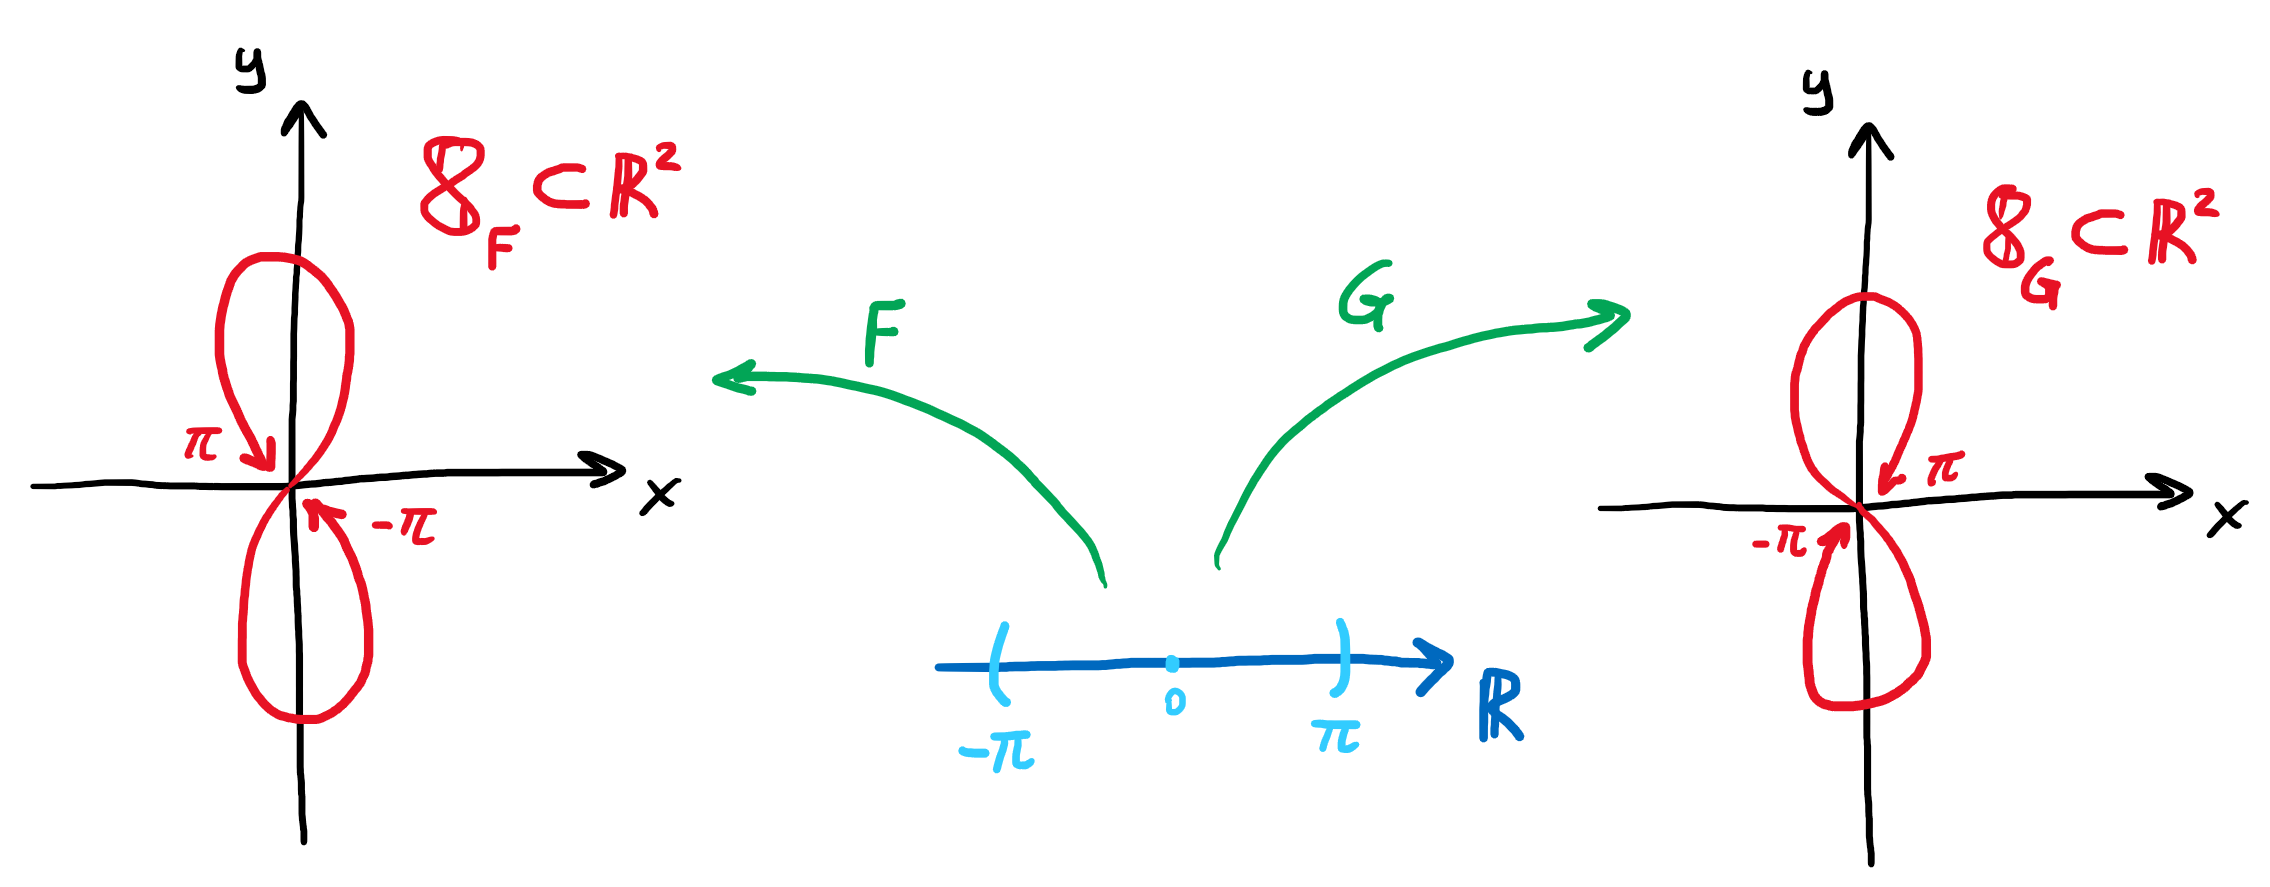
\includegraphics[width=0.8\textwidth,keepaspectratio]{img41}
\end{figure}

Consideriamo ora l'applicazione $ H $ che mappa i punti come $ G $ ma nell'immagine di $ F $, i.e.

\begin{align}
	\begin{split}
		H : (-\pi,\pi) &\to \mathfrak{8}_{F}\\
		t &\mapsto (\sin(2t),-\sin(t))
	\end{split}
\end{align}

il cui codominio possiede la struttura differenziabile indotta da $ G $. Nonostante la funzione $ G $ sia liscia e l'immagine di $ H $ sia contenuta in $ \R^{2} $, $ \mathfrak{8}_{F} $ non è una sottovarietà di $ \R^{2} $ e $ H $ non è nemmeno continua (perciò non liscia): per dimostrarlo è necessario considerare un aperto nel codominio e dimostrare che la sua controimmagine non è aperta nel dominio. Consideriamo dunque l'aperto (segmento) $ U = (a,b) \in \mathfrak{8}_{F} $: la sua controimmagine tramite $ F $ è aperta in $ (-\pi,\pi) $, mentre non è aperta se si prende la sua controimmagine tramite $ H $, i.e.

\begin{equation}
	U = (a,b) \in \mathfrak{8}_{F}%
	\rightarrow%
	\begin{cases}
		F^{-1}(U) = (F^{-1}(a),F^{-1}(b)) & \text{aperta}\\
		H^{-1}(U) = (-\pi,H^{-1}(a)) \cup 0 \cup (H^{-1}(b),\pi) & \text{non aperta}
	\end{cases}
\end{equation}

Il fatto che immagine e preimmagine non siano entrambe aperte rende $ H $ non continua.

\begin{figure}[H]
	\centering
	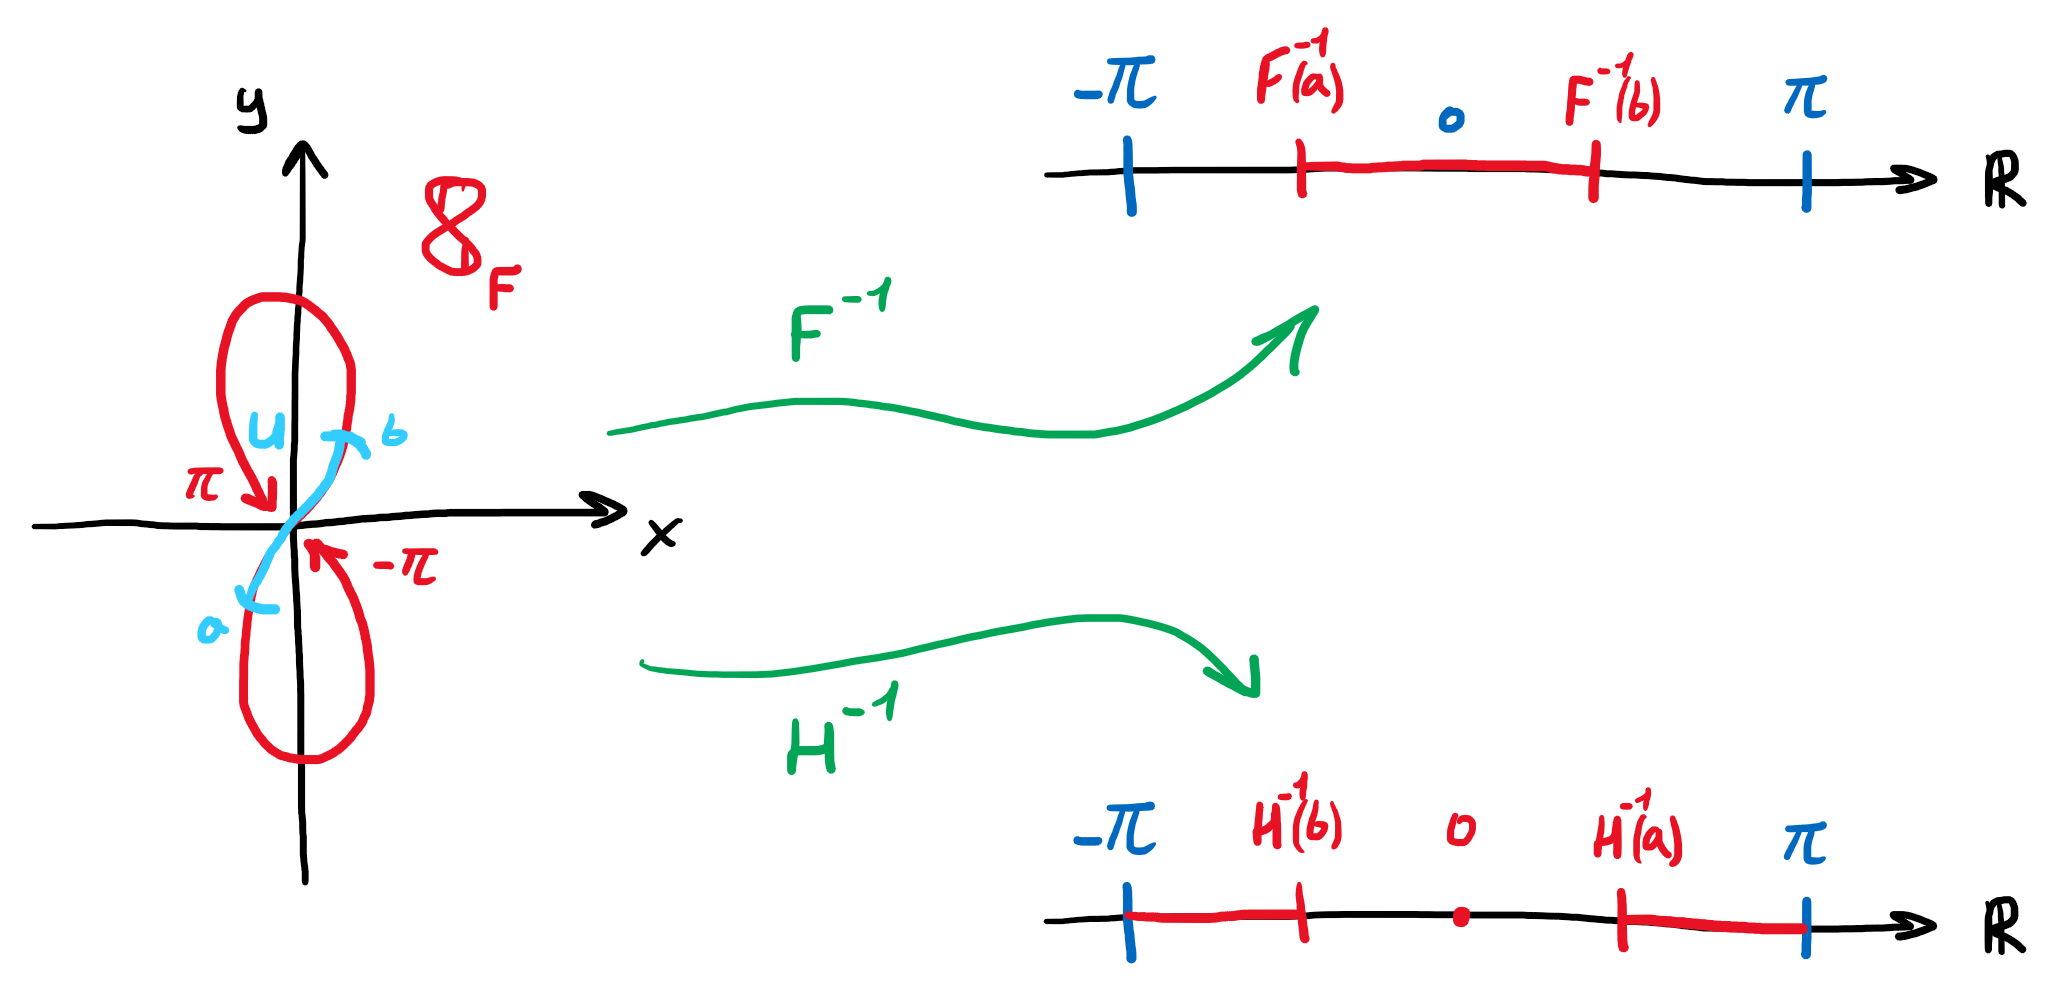
\includegraphics[width=0.8\textwidth,keepaspectratio]{img42}
\end{figure}

Questo esempio mostra come, presa una funzione liscia tra varietà differenziabili, la restrizione del codominio da una varietà a un sottoinsieme (varietà) di questa varietà non è ancora una funzione liscia, a meno che il sottoinsieme della varietà non sia una sottovarietà di questa (quindi con la relativa struttura ereditata): in questo caso, restringere il codominio $ \R^{2} $ della funzione $ G $ alla varietà $ \mathfrak{8}_{F} \subset \R^{2} $ (la quale non è una sottovarietà di $ \R^{2} $) non rende la funzione $ H $ nemmeno continua. Quest'ultimo risultato può essere derivato anche dal fatto che la lemniscata di Bernoulli non sia un sottospazio topologico di $ \R^{2} $.

\paragraph{2. Gruppo lineare speciale}\label{ex-slnr}

Sia l'insieme

\begin{equation}
	SL_{n}(\R) = \{ A \in GL_{n}(\R) \mid \det(A)=1 \} \subset GL_{n}(\R)
\end{equation}

il quale è una sottovarietà di $ GL_{n}(\R) $.\\
Consideriamo l'applicazione del prodotto tra matrici di $ SL_{n}(\R) $

\begin{align}
	\begin{split}
		\mu : SL_{n}(\R) \times SL_{n}(\R) &\to SL_{n}(\R)\\
		(A,B) &\mapsto A B
	\end{split}
\end{align}

e verifichiamo che $ \mu $ sia liscia.\\
Moltiplicare due matrici di $ SL_{n}(\R) $ non è banale, lo sarebbe in $ GL_{n}(\R) $ che ha le carte con gli omeomorfismi verso $ \R^{n^{2}} $, rendendo dunque il prodotto tra matrici una semplice concatenazione di somme e prodotti tra numeri reali.\\
Sia l'applicazione liscia del prodotto tra matrici di $ GL_{n}(\R) $

\begin{align}
	\begin{split}
		F : GL_{n}(\R) \times GL_{n}(\R) &\to GL_{n}(\R)\\
		(A,B) &\mapsto A B
	\end{split}
\end{align}

se restringiamo il dominio a $ SL_{n}(\R) \times SL_{n}(\R) $, otteniamo l'applicazione

\begin{align}
	\begin{split}
		G : SL_{n}(\R) \times SL_{n}(\R) &\to GL_{n}(\R)\\
		(A,B) &\mapsto A B
	\end{split}
\end{align}

definita come $ G = F \circ (i \times i) $ dove $ i : SL_{n}(\R) \to GL_{n}(\R) $ indica l'inclusione: essendo $ F $ e $ i $ lisce (e dunque anche $ i \times i $\footnote{%
	Vedi Esercizio \ref{es2-12}.%
}), anche $ G $ è liscia.\\
Siccome la moltiplicazione di due matrici con determinante unitario è ancora una matrice con determinante unitario, abbiamo che $ G(SL_{n}(\R) \times SL_{n}(\R)) \subset SL_{n}(\R) $ e quindi possiamo restringere il codominio, ottenendo la funzione

\begin{align}
	\begin{split}
		\tilde{G} : SL_{n}(\R) \times SL_{n}(\R) &\to SL_{n}(\R)\\
		(A,B) &\mapsto A B
	\end{split}
\end{align}

la quale è ancora liscia dal teorema. Dalle definizioni, sappiamo che $ \mu \equiv \tilde{G} $ perciò $ \mu $ è liscia.

\section{Il fibrato tangente e i campi di vettori}

\subsection{Fibrato tangente}

Sia $ M $ una varietà differenziabile di dimensione $ n $. Il \textit{fibrato tangente ad} $ M $ è definito come l'unione disgiunta di tutti gli spazi tangenti ai punti di $ M $, i.e.

\begin{equation}
	T(M) \doteq \bigsqcup_{p \in M} T_{p}(M)
\end{equation}

La proiezione naturale è definita come

\begin{align}
	\begin{split}
		\pi : T(M) &\to M\\
		v &\mapsto p
	\end{split}
\end{align}

dove notazioni alternative per $ v \in T_{p}(M) $ sono $ (p,v) $ (per evidenziare il collegamento con il punto $ p \in M $) e $ X_{p} $.\\
Costruiamo ora una struttura differenziabile sul fibrato tangente in modo tale da rendere liscia la proiezione.

\subsubsection{Struttura topologica sul fibrato tangente}

Siano $ U \subset M $ un aperto coordinato, i.e. abbiamo fissato una carta $ (U,\phi) \in M $ intorno a $ p $ con $ \phi = (x^{1},\dots,x^{n}) $, e $ T(U) $ il fibrato tangente a $ U $, dunque

\begin{equation}
	T(U) = \bigsqcup_{p \in M} T_{p}(U) = \bigsqcup_{p \in M} T_{p}(M)
\end{equation}

questo perché $ T_{p}(U) = \der_{p}(C_{p}^{\infty}(U)) $ ma siccome il concetto di germe di funzione è locale

\begin{equation}
	T_{p}(U) = \der_{p}(C_{p}^{\infty}(U)) = \der_{p}(C_{p}^{\infty}(M)) = T_{p}(M)
\end{equation}

Esiste una bigezione naturale tra $ T(U) $ a $ \R^{2n} $: prendendo $ v \in T_{p}(M) $ e sapendo che $ \langle \sfrac{\partial}{\partial x^{i}} |_{p} \rangle = T_{p}(M) $, possiamo scrivere

\begin{equation}
	v = \sum_{i=1}^{n} c^{i}(v) \left. \dfrac{\partial}{\partial x^{i}} \right|_{p}
\end{equation}

e chiamiamo $ c(v) = (c^{1}(v),\dots,c^{n}(v)) $; a questo punto, la bigezione può essere scritta come

\begin{align}
	\begin{split}
		\tilde{\phi} : T(U) &\to \phi(U) \times \R^{n} = \R^{2n}\\
		v &\mapsto (\phi(p),c(v))\\
		&\mapsto (x^{1}(p),\dots,x^{n}(p),c^{1}(v),\dots,c^{n}(v))
	\end{split}
\end{align}

dove $ \phi(U) \subset \R^{n} $. Per poter scrivere l'immagine in funzione di solo $ v $, consideriamo l'applicazione

\begin{align}
	\begin{split}
		\phi_{*} = \phi_{*p} : T_{p}(U) &\to T_{\phi(p)}(\phi(U)) =  T_{\phi(p)}(\R^{n})\\
		\left. \dfrac{\partial}{\partial x^{i}} \right|_{p} &\mapsto \left. \dfrac{\partial}{\partial r^{i}} \right|_{p}
	\end{split}
\end{align}

che applicata a $ v $

\begin{align}
	\begin{split}
		\phi_{*}(v) &= \phi_{*} \left( \sum_{i=1}^{n} c^{i}(v) \left. \dfrac{\partial}{\partial x^{i}} \right|_{p} \right)\\
		&= \sum_{i=1}^{n} c^{i}(v) \phi_{*} \left( \left. \dfrac{\partial}{\partial x^{i}} \right|_{p} \right)\\
		&= \sum_{i=1}^{n} c^{i}(v) \left. \dfrac{\partial}{\partial r^{i}} \right|_{p}
	\end{split}
\end{align}

il quale risultato può essere identificato con $ c(v) = (c^{1}(v),\dots,c^{n}(v)) $ in $ \R^{n} $. Da tutto ciò e considerando $ p = \pi(v) $, si può riscrivere $ \tilde{\phi} $ come

\begin{equation}
	\tilde{\phi}(v) = (\phi \circ \pi,\phi_{*})(v) = (\phi(\pi(v)),\phi_{*}(v))
\end{equation}

Questa applicazione è invertibile (essendo una bigezione) e la sua inversa è

\begin{align}
	\begin{split}
		\tilde{\phi}^{-1} : \phi(U) \times \R^{n} &\to T(U)\\
		(\phi(p),c(v)) &\mapsto v = \sum_{i=1}^{n} c^{i}(v) \left. \dfrac{\partial}{\partial x^{i}} \right|_{p}
	\end{split}
\end{align}

Definiamo dunque la topologia su $ T(U) $ (indotta dall'applicazione $ \tilde{\phi} $) come

\begin{equation}
	A \subset T(U) \text{ aperto} \iff \tilde{\phi}(A) \text{ aperto in } \phi(U) \times \R^{n}
\end{equation}

Abbiamo le seguenti conseguenze:

\begin{itemize}
	\item $ \tilde{\phi} : T(U) \to \phi(U) \times \R^{n} $ è un omeomorfismo;
	
	\item Preso $ V \subset U $, la topologia indotta da $ T(U) $ su $ T(V) $ ($ T(V) \subset T(V) $) è la stessa della topologia indotta su $ T(V) $ dall'applicazione $ \tilde{\phi}_{|T(V)} : T(V) \to \phi(V) \times \R^{n} $.
\end{itemize}

Per costruire una topologia su $ T(M) $ consideriamo dunque l'insieme

\begin{equation}
	\mathcal{B}_{T(M)} = \bigcup_{\alpha} \{ A \subset T(U_{\alpha}) \text{ aperti} \}
\end{equation}

cioè l'unione di tutti gli aperti $ A $ contenuti nei rispettivi $ T(U_{\alpha}) $ al variare di $ \alpha $, dove $ U_{\alpha} $ è un aperto coordinato dell'atlante massimale di $ M $.

\begin{definition}
	L'insieme $ \mathcal{B}_{T(M)} $ è una base per una topologia su $ T(M) $.
\end{definition}

\begin{proof}
	Per la dimostrazione è necessario che
	
	\begin{itemize}
		\item $ \mathcal{B}_{T(M)} $ sia un ricoprimento di $ T(M) $;
		
		\item L'intersezione di due elementi di $ \mathcal{B}_{T(M)} $ si può scrivere come unione di elementi di $ \mathcal{B}_{T(M)} $.
	\end{itemize}

	Per definizione $ T(U_{\alpha}) \in \mathcal{B}_{T(M)} $ in quanto aperto; abbiamo anche che vale la seguente implicazione
	
	\begin{equation}
		\bigcup_{\alpha} U_{\alpha} = M \implies \bigcup_{\alpha} T(U_{\alpha}) = T(M)
	\end{equation}

	perciò $ \mathcal{B}_{T(M)} $ è un ricoprimento di $ T(M) $.\\
	Siano due aperti $ A \subset T(U) $ e $ B \subset T(V) $, i.e. $ A,B \in \mathcal{B}_{T(M)} $, con $ U $ e $ V $ due aperti coordinati (i.e. fanno parte di carte di $ T(U) $ e $ T(V) $ rispettivamente). Dimostrando che $ T(U) \cap T(V) = T(U \cap V) $ tramite
	
	\begin{align}
		\begin{split}
			T(U) \cap T(V) &= \left( \bigsqcup_{p \in U} T_{p}(U) \right) \cap \left( \bigsqcup_{q \in V} T_{p}(V) \right)\\
			&= \left( \bigsqcup_{p \in U} T_{p}(M) \right) \cap \left( \bigsqcup_{q \in V} T_{p}(M) \right)\\
			&= \bigsqcup_{r \in U \cap V} T_{r}(M)\\
			&= \bigsqcup_{r \in U \cap V} T_{r}(U \cap V)\\
			&= T(U \cap V)
		\end{split}
	\end{align}
	
	possiamo scrivere che
	
	\begin{equation}
		A \cap B \subset T(U) \cap T(V) = T(U \cap V)
	\end{equation}

	dove $ U \cap V $ è ancora un aperto coordinato della carta $ (U \cap V,\phi_{|U \cap V}) $. Dobbiamo verificare ora che $ A \cap B \subset T(U \cap V) $ sia aperto in $ T(U \cap V) $ (l'intersezione di due elementi della base si può scrivere come unione di elementi della base) perché $ \mathcal{B}_{T(M)} $ sia effettivamente una base: osserviamo che
	
	\begin{align}
		\begin{split}
			A \cap B &= (A \cap B) \cap T(U \cap V)\\
			&= (A \cap T(U \cap V)) \cap (B \cap T(U \cap V))
		\end{split}
	\end{align}

	perciò, perché $ A \cap B $ sia aperto in $ T(U \cap V) $, è sufficiente che $ A \cap T(U \cap V) $ sia aperto in $ T(U \cap V) $ (risp. per $ B $). Questo è vero perché $ T(U \cap V) \subset T(U) $ e ha la topologia indotta da $ T(U) $ (perché $ U \cap V \subset U $) e i suoi aperti sono gli aperti di $ T(U) $ (e.g. $ A $) intersecati con $ T(U \cap V) $ stesso, i.e. $ A \cap T(U \cap V) $; il ragionamento è analogo per $ B $.
\end{proof}

A questo punto $ T(M) $ è uno spazio topologico con la topologia che ha $ \mathcal{B}_{T(M)} $ come base.\footnote{%
	Questa topologia per $ T(M) $ è l'unica possibile.%
}\\
Dobbiamo far vedere ora che $ T(M) $ è una varietà topologica e per farlo dobbiamo mostrare che sia $ N_{2} $, $ T_{2} $ e localmente euclideo.\\
Useremo il seguente lemma per dimostrare il secondo criterio di numerabilità $ N_{2} $:

\begin{lemma}
	Ogni varietà differenziabile ha una base numerabile di insiemi coordinati o equivalentemente esiste un atlante differenziabile numerabile.
\end{lemma}

\begin{proof}
	Siano $ \{(U_{\alpha},\phi_{\alpha})\} $ l'atlante massimale di $ M $ che definisce la struttura differenziabile di $ M $ e $ \mathfrak{U} = \{U_{i}\}_{i \in I} $ una base numerabile per la topologia di $ M $ (questa esiste in quanto $ M $ è $ N_{2} $).\\
	Presi un punto $ p \in M $ e un aperto $ U_{\alpha} $ di una carta dell'atlante, esiste sempre $ B_{p,\alpha} \in \mathfrak{U} $ tale che $ p \in B_{p,\alpha} \subset U_{\alpha} $, in quanto $ \mathfrak{U} $ è una base. Consideriamo ora la famiglia di aperti $ \mathfrak{B} = \{B_{p,\alpha}\} $ senza duplicati, la quale sarà una sottofamiglia di $ \mathfrak{U} $ e, in quanto tale, sarà numerabile perché $ \mathfrak{U} $ è numerabile. Inoltre $ (B_{p,\alpha}, \phi_{|B_{p,\alpha}}) $ è una carta di $ M $ e dunque $ \{(B_{p,\alpha}, \phi_{|B_{p,\alpha}})\} $ è un atlante differenziabile numerabile per $ M $.\\
	Resta da dimostrare che $ \mathfrak{B} $ sia una base (già numerabile) per $ M $: siano $ p \in M $ e $ U \ni p $ aperto di $ M $, siccome esiste sempre un aperto di una carta che sia contenuto in un aperto della varietà, possiamo scrivere $ p \in U_{\alpha} \subset U $, dove la carta considerata dell'atlante è $ (U \cap U_{\alpha},\phi_{U \cap U_{\alpha}}) $; sappiamo anche che esiste $ B_{p,\alpha} $ tale che $ p \in B_{p,\alpha} \subset U_{\alpha} $, dunque $ p \in B_{p,\alpha} \subset U $. Questo significa che esiste sempre un aperto $ B_{p,\alpha} \in \mathfrak{B} $ che si interponga tra ogni punto della varietà e ogni aperto che contiene il punto stesso, i.e. $ \mathfrak{B} $ è una base per $ M $.
\end{proof}

\paragraph{Localmente euclideo}

Sia $ \{(U_{\alpha},\phi_{\alpha})\} $ un atlante topologico per $ M $, allora $ \{(T(U_{\alpha}),\tilde{\phi}_{\alpha})\} $ è un atlante topologico per $ T(M) $. Questo è vero perché i $ T(U_{\alpha}) $ sono un ricoprimento di $ T(M) $, i.e.

\begin{equation}
	\bigcup_{\alpha} T(U_{\alpha}) = T(M)
\end{equation}

e le applicazioni

\begin{equation}
	\tilde{\phi}_{\alpha} : T(U_{\alpha}) \to \phi_{\alpha}(U_{\alpha}) \times \R^{n}
\end{equation}

sono omeomorfismi in aperti di $ \R^{2n} $, dunque $ \dim(T(M)) = 2 \dim(M) = 2n $.

\paragraph{$ T_{2} $ o di Hausdorff}

Per definizione, un insieme è di Hausdorff se, dati due punti, esistono due intorni disgiunti che contengono questi due punti.\\
Siano $ (p,v) \in T_{p}(M) $ e $ (q,w) \in T_{q}(M) $ due punti distinti di $ T(M) $: presi $ v \neq w $, abbiamo due casi

\begin{itemize}
	\item se $ p = q $ allora $ T_{p}(M) = T_{q}(M) \subset T(U) $ dove $ U $ è un aperto coordinato di $ (U,\phi) \ni p=q $, ma $ T(U) \simeq \phi(U) \times \R^{n} $ dunque $ T(U) $ eredita la proprietà $ T_{2} $ da $ \phi(U) \times \R^{n} $ e a sua volta $ T_{p}(M) = T_{q}(M) $ la eredita da $ T(U) $, i.e.
	
	\begin{equation}
		\E A,B \in T(U) = T(M) \text{ aperti}, \, A \ni (p,v) \wedge B \ni (q,w) \mid A \cap B = \{\}
	\end{equation}
	
	\item se $ p \neq q $, siccome $ M $ è $ T_{2} $ esisteranno due aperti disgiunti coordinati che contengono $ p $ e $ q $, i.e.
	
	\begin{equation}
		\E U,V \in M, \, U \ni p \wedge V \ni q, \, (U,\phi),(V,\psi) \in M \mid U \cap V = \{\}
	\end{equation}

	per cui, siccome $ T(U) \ni (p,v) $ e $ T(V) \ni (q,w) $ e
	
	\begin{equation}
		T(U) \cap T(V) = T(U \cap V) = \{\} \quad \because \quad U \cap V = \{\}
	\end{equation}

	abbiamo che $ T(M) $ è di Hausdorff.
\end{itemize}

\paragraph{$ N_{2} $}

Sia $ \{(U_{i},\phi_{i})\} $ un atlante differenziabile numerabile di $ M $ (la sua esistenza segue dal lemma dimostrato sopra), allora gli omeomorfismi

\begin{equation}
	\tilde{\phi}_{i} : T(U_{i}) \to \phi_{i}(U_{i}) \times \R^{n}
\end{equation}

permettono di dire, siccome $ T(U_{i}) \simeq \phi(U_{i}) \times \R^{n} $ e $ \phi(U_{i}) \times \R^{n} $ è $ N_{2} $, che $ T(U_{i}) $ sia $ N_{2} $.\\
Fissato $ i In I $, sia $ \{B_{ij}\}_{j \in J} $ una base numerabile (con $ I $ e $ J $ numerabili) per $ T(U_{i}) $, allora l'unione

\begin{equation}
	\bigcup_{i \in I, j \in J} \{B_{ij}\}
\end{equation}

è una base numerabile per $ T(M) $ e dunque $ T(M) $ è $ N_{2} $.

\subsubsection{Struttura differenziabile sul fibrato tangente}

Dopo aver dimostrato che $ T(M) $ è una varietà topologica, dimostriamo che è anche una varietà differenziabile con atlante differenziabile $ \{(T(U_{\alpha}),\tilde{\phi}_{\alpha})\}_{\alpha \in A} $ dove $ \{(U_{\alpha},\phi_{\alpha})\}_{\alpha \in A} $ è un atlante differenziabile per $ M $. L'unico fatto da verificare è che le carte siano $ C^{\infty} $-compatibili o equivalentemente che i cambi di carte siano lisci.\\
Considerando che $ U_{\alpha} \cap U_{\beta} = U_{\alpha \beta} $, 

\begin{equation}
	T(U_{\alpha}) \cap T(U_{\beta}) = T(U_{\alpha} \cap U_{\beta}) \doteq T(U_{\alpha \beta})
\end{equation}

possiamo scrivere i cambi di carta come

\begin{align}
	\begin{split}
		\tilde{\phi}_{\beta} \circ \tilde{\phi}_{\alpha}^{-1} : \tilde{\phi}_{\alpha}(T(U_{\alpha \beta})) &\to \tilde{\phi}_{\beta}(T(U_{\alpha \beta}))\\
		\tilde{\phi}_{\alpha} \circ \tilde{\phi}_{\beta}^{-1} : \tilde{\phi}_{\beta}(T(U_{\alpha \beta})) &\to \tilde{\phi}_{\alpha}(T(U_{\alpha \beta}))
	\end{split}
\end{align}

i quali devono essere lisci per $ \forall \alpha,\beta \in A $, dove i $ T(U_{\alpha \beta}) $ sono aperti di $ \R^{2n} $.\\
Scriviamo le singole applicazioni come

\begin{align}
	\begin{split}
		\tilde{\phi}_{\alpha} : T(U_{\alpha}) &\to \phi_{\alpha}(U_{\alpha}) \times \R^{n}\\
		v &\mapsto (\phi_{\alpha} \circ \pi, \phi_{*p})(v)
	\end{split}
\end{align}

dove\footnote{%
Il simbolo $ \longleftrightarrow $ indica l'identificazione.%
}

\begin{equation}
	\begin{cases}
		v = \sum_{i=1}^{n} a^{i}(v) \left. \dfrac{\partial}{\partial x^{i}} \right|_{p}\\
		\pi(v) = p\\
		\phi_{*}(v) = \sum_{i=1}^{n} a^{i}(v) \left. \dfrac{\partial}{\partial r^{i}} \right|_{p} \longleftrightarrow a(v) = (a^{1}(v),\dots,a^{n}(v)) \in \R^{n}
	\end{cases}	
\end{equation}

e la carta utilizzata è $ (U_{\alpha},\phi_{\alpha}) $ con $ \phi_{\alpha} = (x^{1},\dots,x^{n}) $. A questo possiamo riscrivere l'applicazione

\begin{align}
	\begin{split}
		\tilde{\phi}_{\alpha} : T(U_{\alpha}) &\to \phi_{\alpha}(U_{\alpha}) \times \R^{n}\\
		v &\mapsto (\phi_{\alpha} \circ \pi, \phi_{*p})(v)\\
		&\mapsto ( \, x^{1}(\pi(v)),\dots,x^{n}(\pi(v)), a^{1}(v),\dots,a^{n}(v))
	\end{split}
\end{align}

e la sua inversa

\begin{align}
	\begin{split}
		\tilde{\phi}_{\alpha}^{-1} : \phi_{\alpha}(U_{\alpha}) \times \R^{n} &\to T(U_{\alpha})\\
		(\phi_{\alpha}(p), a^{1},\dots,a^{n}) &\mapsto \sum_{i=1}^{n} a^{i}(v) \left. \dfrac{\partial}{\partial x^{i}} \right|_{p}
	\end{split}
\end{align}

Per la funzione $ \tilde{\phi}_{\beta} $ usiamo la carta $ (U_{\beta},\phi_{\beta}) $ con $ \phi_{\beta} = (y^{1},\dots,y^{n}) $ e

\begin{equation}
	\begin{cases}
		v = \sum_{i=1}^{n} b^{i}(v) \left. \dfrac{\partial}{\partial y^{i}} \right|_{p}\\
		\pi(v) = p\\
		\phi_{*}(v) = \sum_{i=1}^{n} b^{i}(v) \left. \dfrac{\partial}{\partial r^{i}} \right|_{p} \longleftrightarrow b(v) = (b^{1}(v),\dots,b^{n}(v)) \in \R^{n}
	\end{cases}	
\end{equation}

da cui

\begin{align}
	\begin{split}
		\tilde{\phi}_{\beta} : T(U_{\beta}) &\to \phi_{\beta}(U_{\beta}) \times \R^{n}\\
		v &\mapsto (\phi_{\beta} \circ \pi, \phi_{*p})(v)\\
		&\mapsto ( \, y^{1}(\pi(v)),\dots,y^{n}(\pi(v)), b^{1}(v),\dots,b^{n}(v))\\\\
		%
		\tilde{\phi}_{\beta}^{-1} : \phi_{\beta}(U_{\beta}) \times \R^{n} &\to T(U_{\beta})\\
		(\phi_{\beta}(p), b^{1},\dots,b^{n}) &\mapsto \sum_{i=1}^{n} b^{i}(v) \left. \dfrac{\partial}{\partial y^{i}} \right|_{p}
	\end{split}
\end{align}

In $ T(U_{\alpha \beta}) $, il vettore $ v $ può essere scritto nei seguenti due modi

\begin{equation}
	v = \sum_{j=1}^{n} a^{j}(v) \left. \dfrac{\partial}{\partial x^{j}} \right|_{p} = \sum_{k=1}^{n} b^{k}(v) \left. \dfrac{\partial}{\partial y^{k}} \right|_{p}
\end{equation}

da cui otteniamo

\begin{align}
	\begin{split}
		v(y^{i}) &= \sum_{j=1}^{n} a^{j}(v) \, \dfrac{\partial y^{i}}{\partial x^{j}} (p)\\
		&= \sum_{k=1}^{n} b^{k}(v) \, \dfrac{\partial y^{i}}{\partial y^{k}} (p)\\
		&= \sum_{k=1}^{n} b^{k}(v) \, \delta^{ik}\\
		&= b^{i}(v)\\\\
		%
		v(x^{i}) &= \sum_{k=1}^{n} b^{k}(v) \, \dfrac{\partial x^{i}}{\partial y^{k}} (p)\\
		&= \sum_{j=1}^{n} a^{j}(v) \, \dfrac{\partial x^{i}}{\partial x^{j}} (p)\\
		&= \sum_{k=1}^{n} a^{j}(v) \, \delta^{ij}\\
		&= a^{i}(v)
	\end{split}
\end{align}

perciò

\begin{align}
	\begin{split}
		b^{i}(v) &= \sum_{k=1}^{n} a^{k}(v) \, \dfrac{\partial y^{i}}{\partial x^{k}} (p)\\
		%
		a^{i}(v) &= \sum_{k=1}^{n} b^{k}(v) \, \dfrac{\partial x^{i}}{\partial y^{k}} (p)
	\end{split}
\end{align}

Possiamo dunque scrivere i cambi di carte

\begin{align}
	\begin{split}
		(\tilde{\phi}_{\beta} \circ \tilde{\phi}_{\alpha}^{-1}) (\phi_{\alpha}(p), a^{1},\dots,a^{n}) &= \tilde{\phi}_{\beta} \left( p, \sum_{i=1}^{n} a^{i}(v) \left. \dfrac{\partial}{\partial x^{i}} \right|_{p} \right)\\
		&= \tilde{\phi}_{\beta} \left( p, v = \sum_{i=1}^{n} a^{i}(v) \left. \dfrac{\partial}{\partial x^{i}} \right|_{p} \right)\\
		&= ( \phi_{\beta}(p), b^{1}(v),\dots,b^{n}(v) )\\
		&= \left( (\phi_{\beta} \circ \phi_{\alpha}^{-1})(\phi_{\alpha}(p)), \sum_{i=1}^{n} a^{k}(v) \, \dfrac{\partial y^{1}}{\partial x^{k}} (p) ,\dots, \sum_{i=1}^{n} a^{k}(v) \, \dfrac{\partial y^{n}}{\partial x^{k}} (p) \right)
	\end{split}
\end{align}

ricordando che le entrate della matrice jacobiana sono equivalenti a

\begin{equation}
	\dfrac{\partial y^{j}}{\partial x^{k}} (p) = \dfrac{\partial (\phi_{\beta} \circ \phi_{\alpha}^{-1})^{j}}{\partial r^{k}} (\phi(p))
\end{equation}

otteniamo, applicando un ragionamento analogo per il cambio di carte inverso, le seguenti uguaglianze

\begin{multline}
	(\tilde{\phi}_{\beta} \circ \tilde{\phi}_{\alpha}^{-1}) (\phi_{\alpha}(p), a^{1},\dots,a^{n}) =\\
	= \left( (\phi_{\beta} \circ \phi_{\alpha}^{-1})(\phi_{\alpha}(p)), \sum_{i=1}^{n} a^{k}(v) \, \dfrac{\partial (\phi_{\beta} \circ \phi_{\alpha}^{-1})^{1}}{\partial r^{k}} (\phi_{\alpha}(p)) ,\dots, \sum_{i=1}^{n} a^{k}(v) \, \dfrac{\partial (\phi_{\beta} \circ \phi_{\alpha}^{-1})^{n}}{\partial r^{k}} (\phi_{\alpha}(p)) \right)
\end{multline}

\begin{multline}
	(\tilde{\phi}_{\alpha} \circ \tilde{\phi}_{\beta}^{-1}) (\phi_{\beta}(p), b^{1},\dots,b^{n}) =\\
	= \left( (\phi_{\alpha} \circ \phi_{\beta}^{-1})(\phi_{\beta}(p)), \sum_{i=1}^{n} b^{k}(v) \, \dfrac{\partial (\phi_{\alpha} \circ \phi_{\beta}^{-1})^{1}}{\partial r^{k}} (\phi_{\beta}(p)) ,\dots, \sum_{i=1}^{n} b^{k}(v) \, \dfrac{\partial (\phi_{\alpha} \circ \phi_{\beta}^{-1})^{n}}{\partial r^{k}} (\phi_{\beta}(p)) \right)
\end{multline}

Questi cambi di carte sono lisci perché

\begin{itemize}
	\item per le prime $ n $ componenti $ (\phi_{\alpha} \circ \phi_{\beta}^{-1})(\phi_{\beta}(p)) $: $ \phi_{\beta} \circ \phi_{\alpha}^{-1} $ e $ \phi_{\alpha} \circ \phi_{\beta}^{-1} $ sono i cambi di carte in $ M $ tra $ (U_{\alpha},\phi_{\alpha}) $ e $ (U_{\beta},\phi_{\beta}) $;
	
	\item per le seconde $ n $ componenti: le derivate parziali dei cambi di carte applicate ai punti $ \phi_{\alpha}(p) $ e $ \phi_{\beta}(p) $ moltiplicate per numeri reali $ a^{i} $ e $ b^{i} $ e sommate tra loro sono ancora lisce
\end{itemize}

Questo mostra che $ T(M) $ è una varietà differenziabile di dimensione $ 2n $.

\subsubsection{Proiezione dal fibrato tangente}

Dimostriamo ora che la proiezione dal fibrato tangente di una varietà alla varietà stessa, i.e.

\begin{align}
	\begin{split}
		\pi : T(M) &\to M\\
		(p,v) &\mapsto p
	\end{split}
\end{align}

è liscia: per mostrarlo, prendiamo due carte arbitrarie e facciamo vedere che l'espressione locale è liscia.\\
Siano le carte $ (U,\phi) \in M $ intorno a $ p $ con $ \phi = (x^{1},\dots,x^{n}) $ e $ (T(U),\tilde{\phi}) \in T(M) $ intorno a $ (p,v) \in T_{p}(M) $, dove

\begin{equation}
	v = \sum_{i=1}^{n} c^{i}(v) \left. \dfrac{\partial}{\partial x^{i}} \right|_{p}
\end{equation}

con $ c(v) = (c^{1}(v),\dots,c^{n}(v)) $. Ricordando l'applicazione $ \tilde{\phi} $

\begin{equation}
	\tilde{\phi}(p,v) = (\phi(p),c(v)) = (x^{1}(p),\dots,x^{n}(p),c^{1}(v),\dots,c^{n}(v))
\end{equation}

abbiamo che

\begin{equation}
	(\phi \circ \pi \circ \tilde{\phi}^{-1}) (\phi(p),c^{1},\dots,c^{n}) = (\phi \circ \pi) \left( p, \sum_{i=1}^{n} c^{i} \left. \dfrac{\partial}{\partial x^{i}} \right|_{p} \right) = \phi(p)
\end{equation}

dunque $ \pi $ è localmente liscia (e anche lineare) in quanto proiezione sulle prime $ n $ coordinate e perciò è liscia dappertutto.

\subsection{Funzioni a campana}

Siano $ M $ una varietà differenziabile e $ f : M \to \R $ un'applicazione su varietà (non necessariamente liscia). Definiamo il \textit{supporto di} $ f $, indicato con $ \operatorname{supp}(f) $, come il sottoinsieme di $ M $ costituito dalla chiusura dell'insieme dei punti dove $ f $ non si annulla, i.e. preso l'insieme dei punti dove la funzione si annulla

\begin{equation}
	Z(f) = \{ p \in M \mid f(p) = 0 \}
\end{equation}

se $ M \setminus Z(f) \doteq Z(f)^{C} $, possiamo scrivere

\begin{equation}
	\operatorname{supp}(f) = \overline{Z(f)^{C}}
\end{equation}

Ad esempio, per la funzione 

\begin{figure}[H]
	\centering
	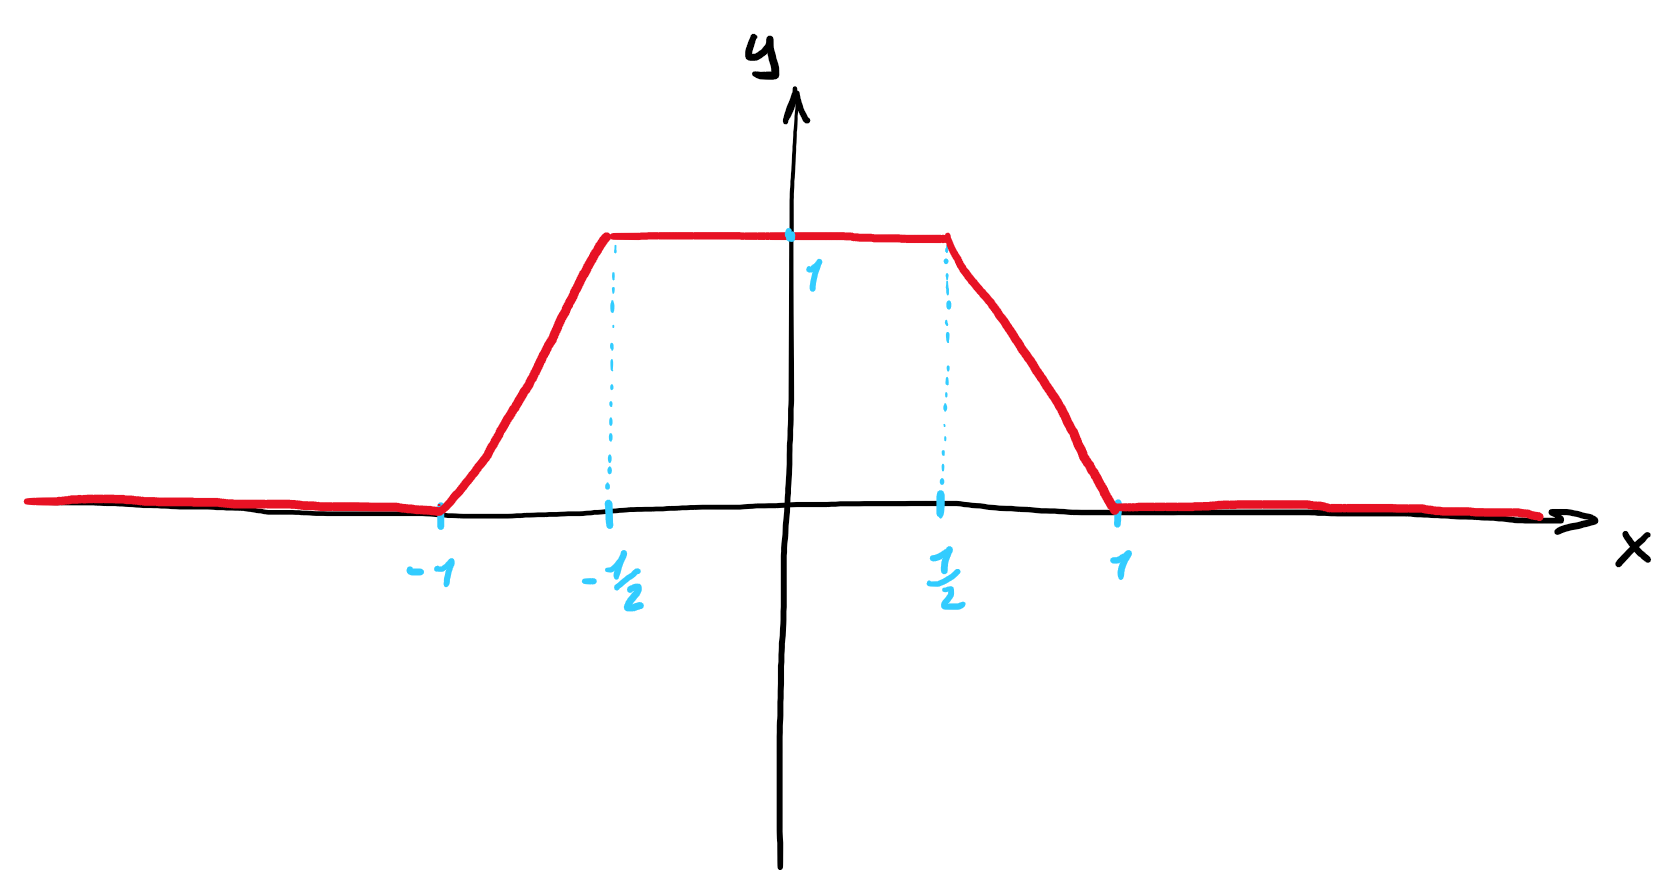
\includegraphics[width=0.7\textwidth,keepaspectratio]{img43}
\end{figure}

\begin{gather}
	Z(f) = (-\infty,-1] \cup [1,+\infty)\\
	Z(f)^{C} = (-1,-1)\\
	\operatorname{supp}(f) = \overline{Z(f)^{C}} = [-1,1]
\end{gather}

O ancora per la funzione

\begin{align}
	\begin{split}
		f : (-1,1) &\to \R\\
		x &\mapsto \tan(\dfrac{\pi x}{2})
	\end{split}
\end{align}

\begin{figure}[H]
	\centering
	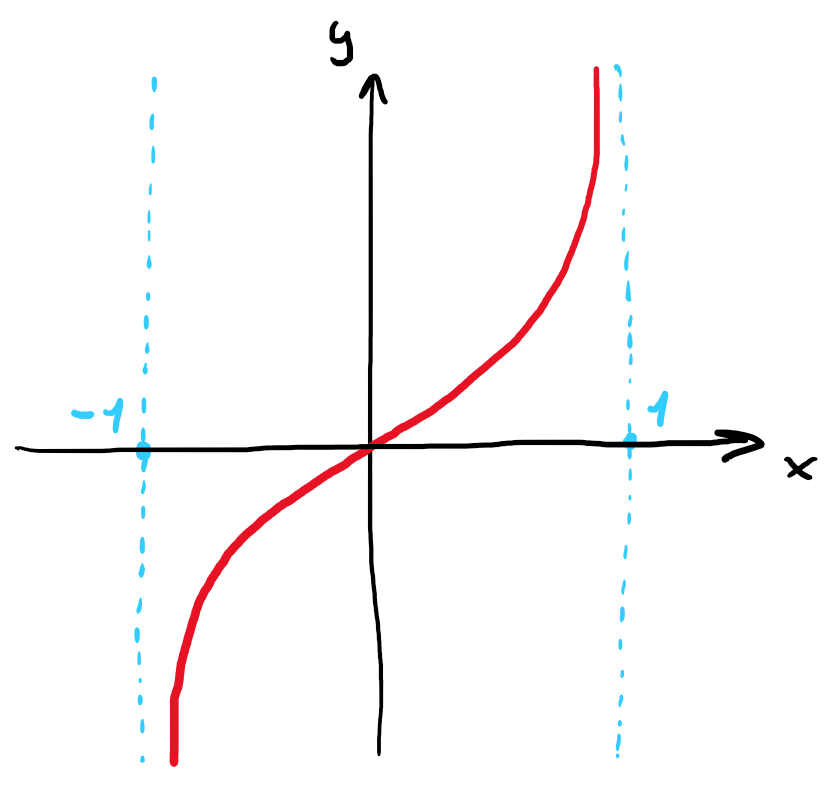
\includegraphics[width=0.3\textwidth,keepaspectratio]{img44}
\end{figure}

\begin{gather}
	Z(f) = \{0\}\\
	Z(f)^{C} = (-1,0) \cup (0,1)\\
	\operatorname{supp}(f) = \overline{Z(f)^{C}} = (-1,1)
\end{gather}

In quanto $ (-1,1) = M $ è chiuso in $ M $.\\\\
%
Siano $ M $ una varietà differenziabile, $ U \subset M $ un aperto della varietà e $ q \in U $ un suo punto, l'applicazione $ f : M \to \R $ è una \textit{funzione a campana}\footnote{%
	In inglese "bump function".%
} in $ q $ con supporto in $ U $ se

\begin{itemize}
	\item $ f $ è continua
	
	\item $ f \equiv 1 $ in un intorno di $ q $
	
	\item $ \operatorname{supp}(f) \subset U $
\end{itemize}

Il primo esempio descritto sopra è una funzione a campana in un qualsiasi punto appartenente a $ (-1,1) $ con supporto in qualunque aperto $ U \supset [-1,1] $.\\\\
%
Partendo da una funzione liscia da $ \R $ in $ \R $, costruiremo una funzione a campana liscia da $ \R^{n} $ a $ \R $.\\
Consideriamo quindi la funzione liscia

\begin{align}
	\begin{split}
		f : \R &\to \R\\
		x &\mapsto%
		\begin{cases}
			e^{\sfrac{-1}{x}} & x > 0\\
			0 & x \leqslant 0
		\end{cases}
	\end{split}
\end{align}

\begin{figure}[H]
	\centering
	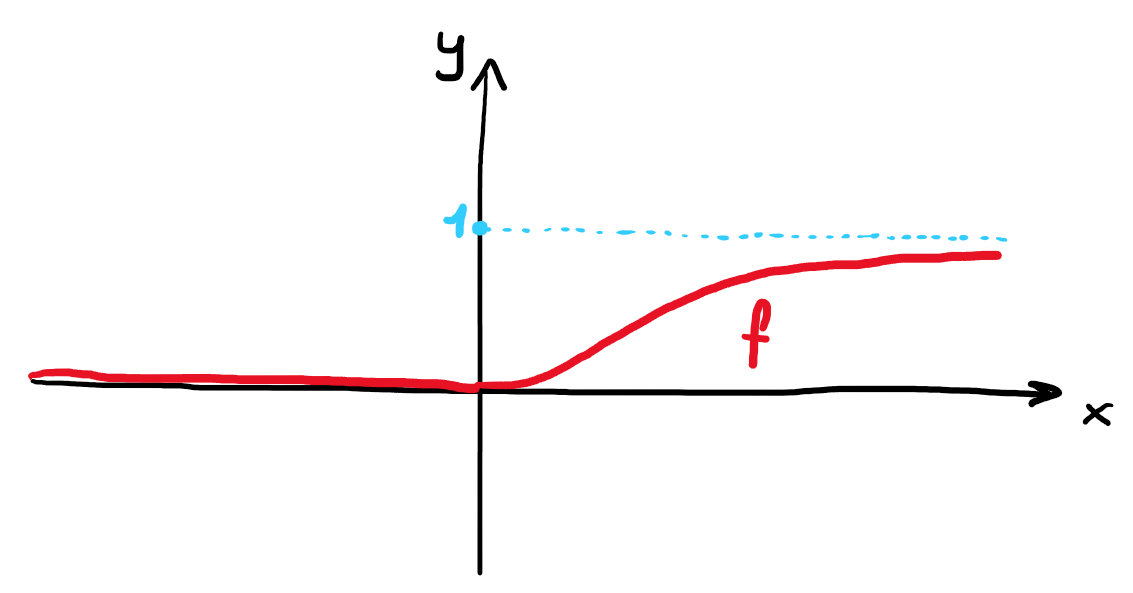
\includegraphics[width=0.5\textwidth,keepaspectratio]{img45}
\end{figure}

Il primo passo è definire una nuova funzione $ g $ a partire da $ f $ come


\begin{equation}
	g(x) = \dfrac{f(x)}{f(x) + f(1-x)}
\end{equation}

questa sarà ancora liscia se il denominatore non si annulla, in quanto

\begin{equation}
	\begin{cases}
		x \leqslant 0 \implies f(x) + f(1-x) = f(1-x) \neq 0 \quad \because \quad 1-x \geqslant 0\\
		x > 0 \implies f(x) + f(1-x) \geqslant f(x) > 0
	\end{cases}
\end{equation}

Se consideriamo il caso

\begin{equation}
	x \geqslant 1 \implies 1-x \leqslant 0 \implies f(1-x)=0 \implies g(x) = \dfrac{f(x)}{f(x)} \equiv 1
\end{equation}

perciò il grafico di $ g(x) $ avrà la forma

\begin{figure}[H]
	\centering
	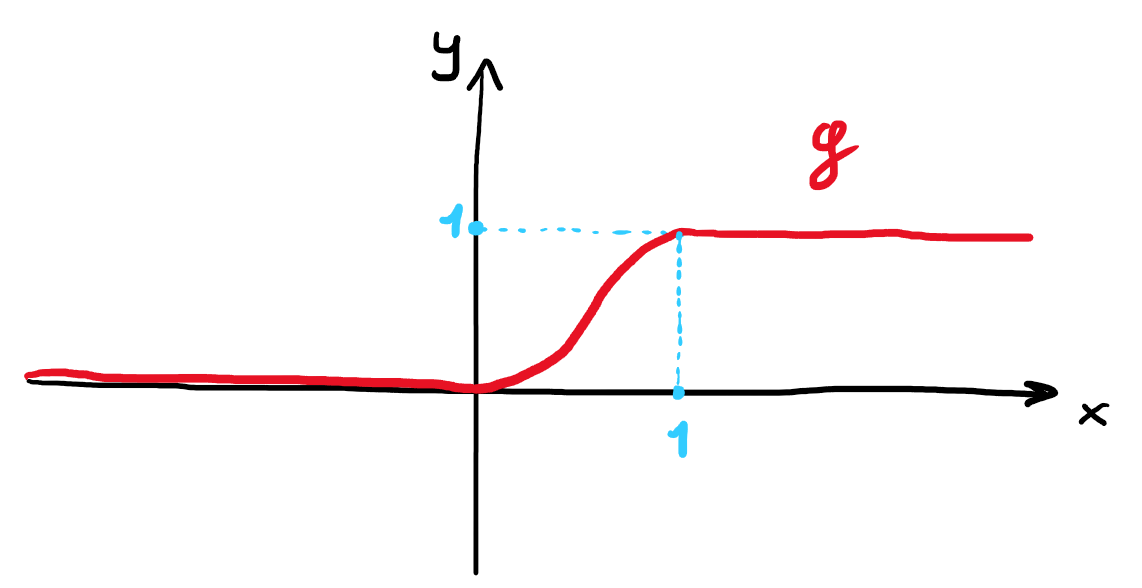
\includegraphics[width=0.5\textwidth,keepaspectratio]{img46}
\end{figure}

In modo tale da poter spostare i punti di contatto, introduciamo la seguente modifica

\begin{equation}
	h(x) = g \left( \dfrac{x - a^{2}}{b^{2} - a^{2}} \right)
\end{equation}

dove $ a,b \in \R $ e $ 0 < a < b $, perciò

\begin{equation}
	\begin{cases}
		h(x) = 1 & x \geqslant b^{2}\\
		h(x) = 0 & x \leqslant a^{2}
	\end{cases}
\end{equation}

da cui la forma "spostata"

\begin{figure}[H]
	\centering
	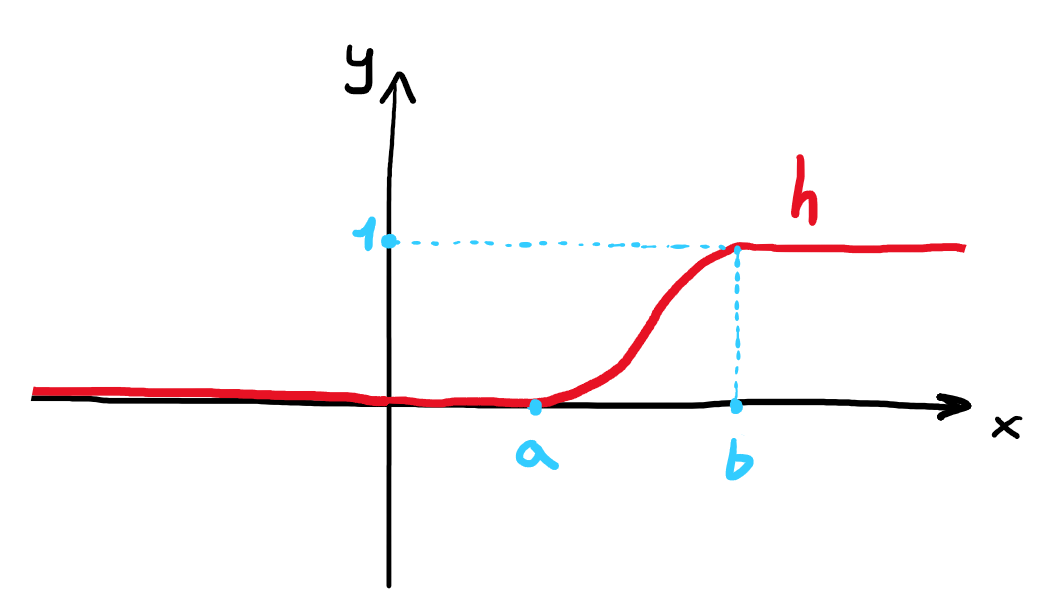
\includegraphics[width=0.5\textwidth,keepaspectratio]{img47}
\end{figure}

Il prossimo passo è rendere la funzione simmetrica

\begin{equation}
	k(x) = h(x^{2})
\end{equation}

perciò

\begin{equation}
	\begin{cases}
		k(x) = 1 & x \leqslant -b \wedge x \geqslant b\\
		k(x) = 0 & -a \leqslant x \leqslant a
	\end{cases}
\end{equation}

da cui la forma a "scodella"

\begin{figure}[H]
	\centering
	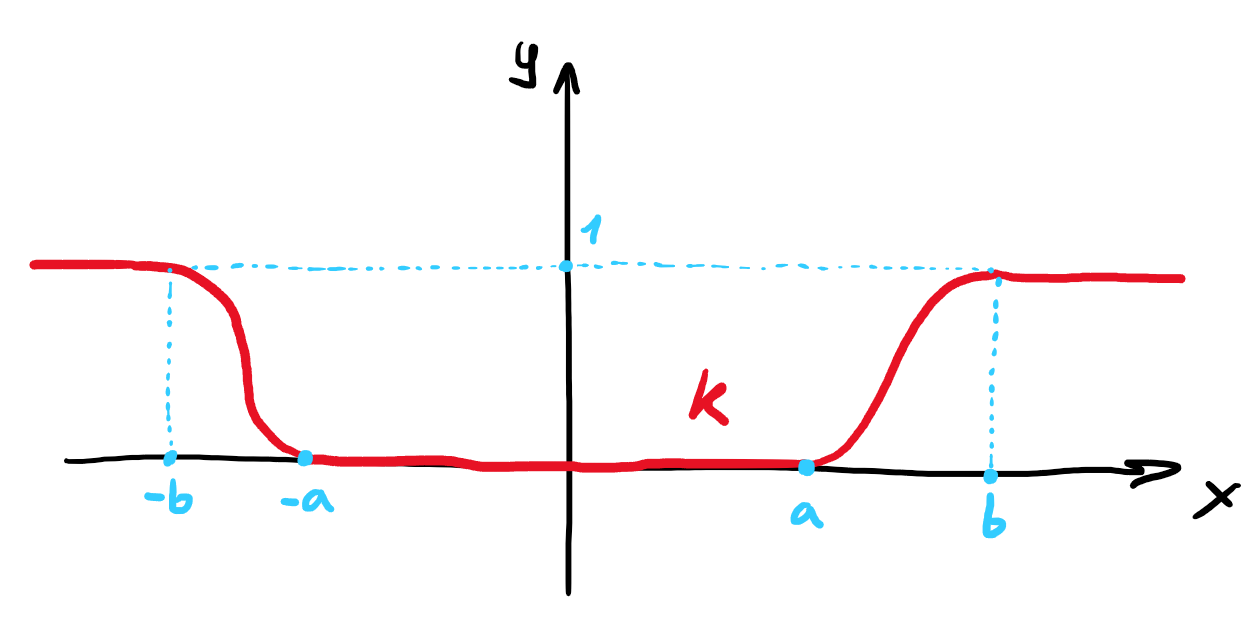
\includegraphics[width=0.5\textwidth,keepaspectratio]{img48}
\end{figure}

Considerando ora l'immagine speculare rispetto all'asse $ x $ e spostata di un'unità verso l'alto

\begin{equation}
	\sigma(x) = 1 - k(x)
\end{equation}

\begin{figure}[H]
	\centering
	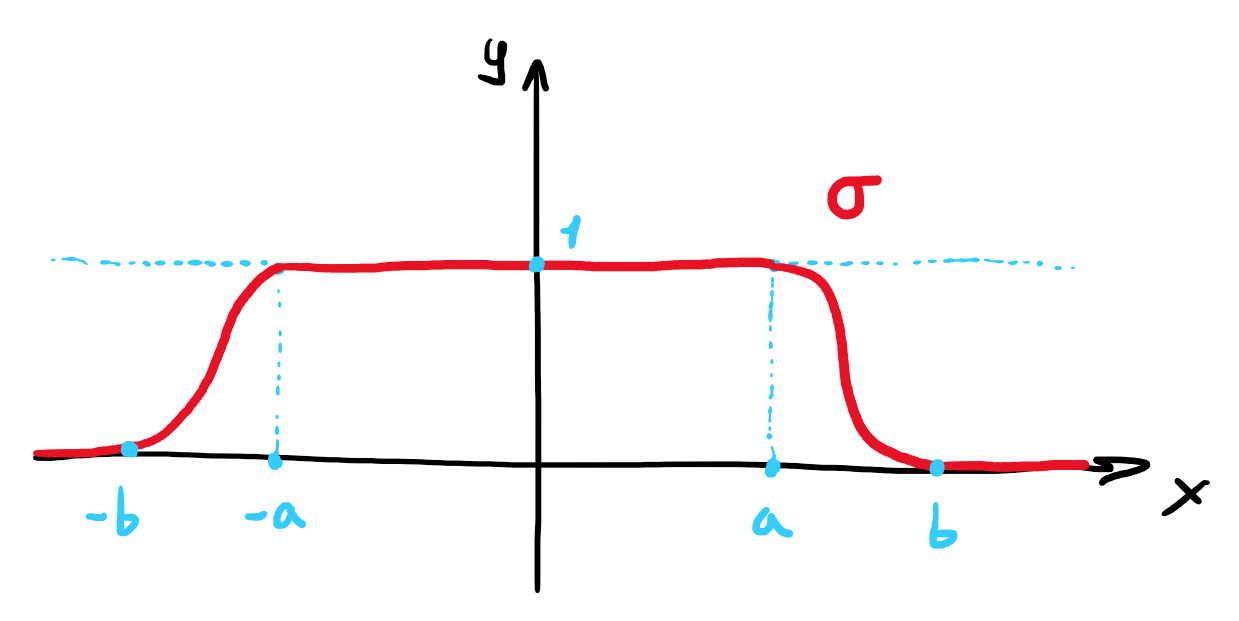
\includegraphics[width=0.5\textwidth,keepaspectratio]{img49}
\end{figure}

A questo punto, generalizziamo al dominio in $ \R^{n} $ considerando $ x = (x^{1},\dots,x^{n}) $ e poi la norma di $ x $

\begin{align}
	\begin{split}
		\rho : \R^{n} &\to \R\\
		x &\mapsto \sigma(\norm{x})
	\end{split}
\end{align}

da cui la forma in $ n+1 $ dimensioni:

\begin{figure}[H]
	\centering
	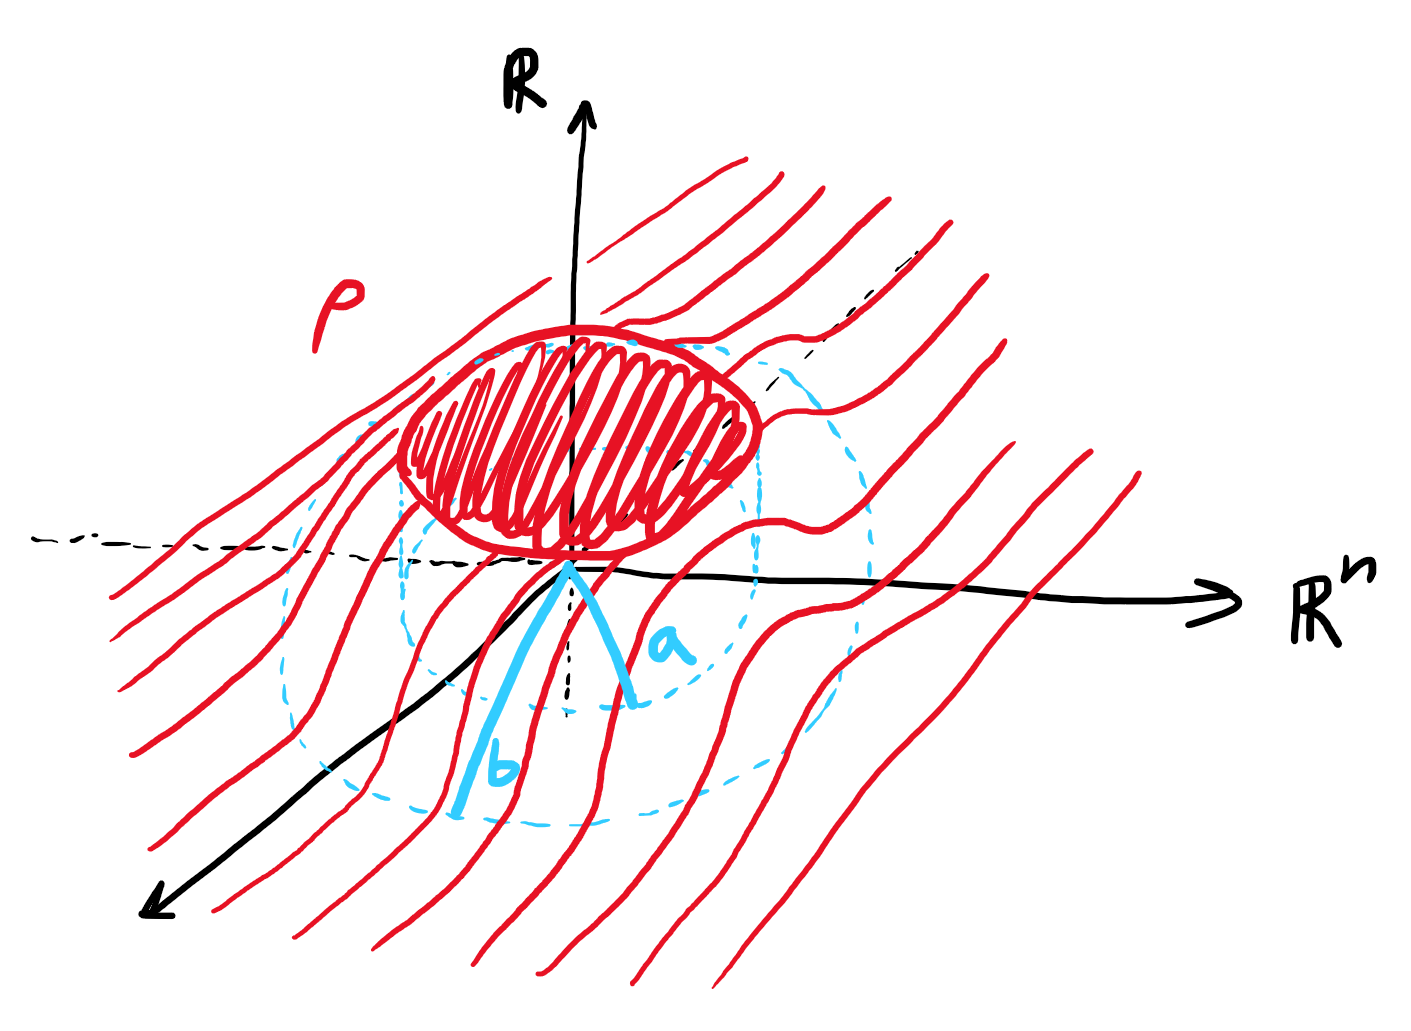
\includegraphics[width=0.5\textwidth,keepaspectratio]{img50}
\end{figure}

Considerando il disco centrato in $ q $ di raggio $ r $

\begin{equation}
	D_{r}(q) = \{ x \in \R^{n} \mid \norm{x - q} < r \}
\end{equation}

abbiamo che $ \rho $ è una funzione a campana liscia in qualsiasi punto in $ D_{a}(0) $ con supporto $ U $, dove $ U $ è un qualunque aperto tale che $ U \supset \overline{D_{b}(0)} $. I valori principali assunti dalla funzione sono per

\begin{equation}
	\begin{cases}
		\rho(x) = 1 & \forall x \in \overline{D_{a}(0)}\\\\
		\rho(x) = 0 & \forall x \in \R^{n} \setminus D_{b}(0)
	\end{cases}
\end{equation}

Si può spostare il centro della funzione in un punto $ q \in \R^{n} $ tramite la sostituzione

\begin{equation}
	\rho(x) \to \rho(x-q)
\end{equation}

Per la generalizzazione di questo procedimento a funzioni a campana su varietà, consideriamo il seguente teorema:

\begin{theorem}\label{bump-fun}
	Siano $ M $ una varietà differenziabile di dimensione $ n $, $ U \subset M $ un aperto della varietà e $ q \in U $ un suo punto, allora esiste una funzione a campana liscia $ \rho : M \to \R $ in $ q $ con supporto contenuto in $ U $.
\end{theorem}

\begin{proof}
	L'idea è di spostare il problema al costruire la funzione a campana in $ \R^{n} $.\\
	Consideriamo una carta $ (V_{r},\phi) \in M $ tale che
	
	\begin{equation}
		\begin{cases}
			q \in V_{r} \subset U\\
			\phi(q) = 0\\
			\phi(V_{r}) = D_{r}(0) \in \R^{n}
		\end{cases}
	\end{equation}

	ricordando che $ \phi $ è un diffeomorfismo e che è sempre possibile restringere l'aperto $ V_{r} $ in modo tale da avere come immagine il disco considerato.\\
	Consideriamo ora due numeri reali $ a < b < r $ e i dischi in $ \R^{n} $ centrati in 0 che hanno questi come raggio, i.e. $ D_{a}(0) \subset D_{b}(0) \subset D_{r}(0) $ dove $ \phi^{-1}(D_{a}(0)) = V_{a} $ e $ \phi^{-1}(D_{b}(0)) = V_{b} $ da cui $ V_{a} \subset V_{b} \subset V_{r} $.
	
	\begin{figure}[H]
		\centering
		\includegraphics[width=0.8\textwidth,keepaspectratio]{img51}
	\end{figure}	
	
	Presa la funzione a campana su $ \R^{n} $
	
	\begin{equation}
		\begin{cases}
			\sigma : \R^{n} \to \R\\
			\sigma(x) = 1 & \forall x \in \overline{D_{a}(0)}\\
			\sigma(x) = 0 & \forall x \in \R^{n} \setminus D_{b}(0)\\
			\operatorname{supp}(\sigma) = \overline{D_{b}(0)}
		\end{cases}
	\end{equation}

	possiamo definire la funzione su $ M $ per $ p \in M $
	
	\begin{align}
		\begin{split}
			\rho : M &\to \R\\
			p &\mapsto %
			\begin{cases}
				(\sigma \circ \phi)(p) & p \in V_{r}\\
				0 & p \in M \setminus \overline{V_{b}}
			\end{cases}
		\end{split}
	\end{align}

	A questo punto dimostriamo che $ \rho $ sia una funzione a campana liscia in $ q $ con supporto contenuto in $ U $: è necessario che l'applicazione sia liscia, che esista un intorno in cui questa è pari ad 1 e che il suo supporto sia contenuto in $ U $.
	
	\begin{itemize}
		\item Perché questa applicazione sia liscia è necessario che sia liscia per i due casi della definizione (definite in aperti) e che i valori dei due casi coincidano nell'intersezione degli aperti in cui sono definiti (la quale è ancora un aperto), i.e.
		
		\begin{equation}
			\begin{cases}
				\sigma \circ \phi \in C^{\infty}(V_{r})\\
				0 \in C^{\infty} \left( M \setminus \overline{V_{b}} \right)\\
				(\sigma \circ \phi)(p) = 0 & \forall p \in V_{r} \cap (M \setminus \overline{V_{b}})
			\end{cases}
		\end{equation}
		
		La seconda richiesta è banale e la prima è soddisfatta in quanto composizione di funzioni lisce; per la terza, possiamo scrivere
		
		\begin{equation}
			V_{r} \cap \left( M \setminus \overline{V_{b}} \right) = V_{r} \setminus \overline{V_{b}}
		\end{equation}
		
		essendo $ \sigma(x) = 0 $ per $ \forall x \in \R^{n} \setminus D_{b}(0) $, possiamo dunque scrivere
		
		\begin{equation}
			(\sigma \circ \phi)(p) = 0, \qquad \forall p \in V_{r} \setminus \overline{V_{b}}
		\end{equation}
		
		%
		
		\item Abbiamo che $ V_{a} \ni q $ e che
		
		\begin{equation}
			\rho(p) \equiv 1, \qquad \forall p \in V_{a}
		\end{equation}
	
		perciò esiste un intorno di $ q $ (in questo caso $ V_{a} $) in cui la funzione è pari ad 1
		
		%
		
		\item Abbiamo che
		
		\begin{equation}
			\operatorname{supp}(\sigma) = \overline{D_{b}(0)}
		\end{equation}
	
		e che $ \phi $ è un diffeomorfismo, dunque il supporto di $ \rho $ sarà
		
		\begin{equation}
			\operatorname{supp}(\rho) = \phi \left( \overline{D_{b}(0)} \right) = \overline{V_{b}} \subset V_{r} \subset U
		\end{equation}
	\end{itemize}
	
	Questo prova dunque che esiste una funzione a campana liscia per ogni punto di una varietà con supporto contenuto in un intorno del punto.
\end{proof}

\begin{corollary}[Estensione di funzioni lisce]\label{cor-est-smooth}
	Siano $ M $ una varietà differenziabile, un punto $ p \in M $, un aperto $ U \subset M $ che sia intorno di $ p $ e una funzione $ f : M \to \R $ liscia solo su $ U $, i.e. $ f \in C^{\infty}(U) $, allora esistono un aperto $ V \subseteq U $ intorno di $ q $ e una funzione $ \tilde{f} : M \to \R $ liscia in tutta la varietà $ \tilde{f} \in C^{\infty}(M) $ tale che $ \tilde{f} \equiv f $ in $ V $; in pratica, $ \tilde{f} $ è un'estensione di $ f_{|V} $.
\end{corollary}

In generale non si può estendere una funzione oltre al dominio in cui essa è liscia però, tramite questo corollario, è possibile considerare la restrizione ad un aperto di questa funzione ed estenderla in modo liscio. Un esempio è la funzione $ f(x) = \tan(\sfrac{x}{2}) $ la quale ha due asintoti verticali in $ \pm \pi $: prendendo un aperto $ V \subset [-\pi,\pi] $ e la restrizione di $ f $ ad esso, è possibile "incollare" in modo liscio alla funzione due estensioni di questa oltre il suo dominio.

\begin{proof}
	Sia $ \rho : M \to \R $ una funzione liscia a campana in $ q $ con supporto contenuto in $ U $ (esiste per il teorema precedente) che sia uguale ad 1 nell'aperto $ V $.\\
	Definiamo
	
	\begin{align}
		\begin{split}
			\tilde{f} : M &\to \R\\
			p &\mapsto %
			\begin{cases}
				(\rho \circ f)(p) & p \in U\\
				0 & p \in M \setminus \operatorname{supp}(\rho)
			\end{cases}
		\end{split}
	\end{align}

	Perché sia liscia è necessario che lo sia nei due casi della definizione e che questi coincidano nella loro intersezione: per quest'ultima richiesta, possiamo scrivere l'intersezione come
	
	\begin{equation}
		U \cap (M \setminus \operatorname{supp}(\rho)) = U \setminus \operatorname{supp}(\rho)
	\end{equation}

	la quale è aperta perché il supporto è un chiuso, dunque resta verificare che i casi coincidano, ricordando che
	
	\begin{equation}
		\rho(p) = 0, \qquad \forall p \in M \setminus \operatorname{supp}(\rho)
	\end{equation}

	perciò
	
	\begin{equation}
		\tilde{f}(p) = (\rho \circ f)(p) = 0, \qquad \forall p \in U \setminus \operatorname{supp}(\rho)
	\end{equation}

	dunque la funzione è liscia dappertutto.\\
	L'altra richiesta è che $ \tilde{f} \equiv f $ in $ V $: anche questo è verificato perché
	
	\begin{equation}
		\rho(p) \equiv 1, \quad \forall p \in V \implies \tilde{f}(p) = (\rho \circ f)(p) \equiv f(p), \quad \forall p \in V
	\end{equation}
\end{proof}

\subsection{Campi di vettori su varietà}

Sia $ M $ una varietà differenziabile di dimensione $ m $. Ricordando la definizione del fibrato tangente

\begin{equation}
	T(U) = \bigsqcup_{p \in M} T_{p}(M)
\end{equation}

e della proiezione preso un vettore $ (p,v) \equiv X_{p} \in T_{p}(M) $

\begin{align}
	\begin{split}
		\pi : T(M) &\to M\\
		X_{p} &\mapsto p
	\end{split}
\end{align}

un \textit{campo di vettori} è un'applicazione

\begin{align}
	\begin{split}
		X : M &\to T(M)\\
		p &\mapsto X_{p}
	\end{split}
\end{align}

e dunque $ \pi \circ X = \id_{M} $.\\\\
%
Localmente, un campo di vettori $ X $ su una varietà $ M $ è \textit{liscio} se per $ \forall p \in M $ esiste una carta $ (U,\phi) \in M $ con $ \phi = (x^{1},\dots,x^{n}) $ intorno a $ p $ tale che, scrivendo il vettore $ X_{p} \in T_{p}(M) $ tangente alla varietà $ M $ nel punto $ p \in U $ come

\begin{equation}
	X_{p} = \sum_{j=1}^{n} a^{j}(p) \left. \dfrac{\partial}{\partial x^{j}} \right|_{p} 
\end{equation}

le funzioni $ a^{j} : U \to \R $ sono lisce in $ U $, da cui l'espressione locale dei vettori del campo

\begin{equation}
	X_{|U} = \sum_{j=1}^{n} a^{j} \dfrac{\partial}{\partial x^{j}}
\end{equation}

La definizione non dipende dalla carta scelta: presa un'altra carta $ (V,\psi) \in M $ con $ \psi = (y^{1},\dots,y^{n}) $ intorno a $ p $, $ X_{p} $ si scriverà come

\begin{equation}
	X_{|V} = \sum_{j=1}^{n} b^{j} \dfrac{\partial}{\partial y^{j}} 
\end{equation}

nell'intersezione degli aperti delle carte, i.e. $ U \cap V $, possiamo dunque scrivere che

\begin{align}
	\begin{split}
		a^{j} &= \sum_{j=1}^{n} b^{k} \, \dfrac{\partial x^{j}}{\partial y^{k}}\\
		b^{j} &= \sum_{j=1}^{n} a^{k} \, \dfrac{\partial y^{j}}{\partial x^{k}}
	\end{split}
\end{align}

per $ \forall j=1,\dots,n $, da cui

\begin{equation}
	a^{j} \in C^{\infty}(U) \iff b^{j} \in C^{\infty}(V)
\end{equation}

perché lo sono le entrate delle matrici jacobiane sono lisce.\\\\
%
\`{E} possibile definire un campo liscio anche mediante la seguente proposizione:

\begin{definition}
	Sia $ X $ un campo di vettori su $ M $, allora $ X : M \to T(M) $ è un'applicazione liscia se e solo se il campo di vettori è liscio, i.e. se scrivendo
	
	\begin{equation}
		X_{|U} = \sum_{j=1}^{n} a^{j} \dfrac{\partial}{\partial x^{j}}
	\end{equation}

	si ha che $ a^{j} \in C^{\infty}(U) $.
\end{definition}

\begin{proof}[Dimostrazione ($ \implies $)]
	Siano $ X : M \to T(M) $ un'applicazione liscia e $ (U,\phi) \in M $ con $ \phi = (x^{1},\dots,x^{n}) $ intorno a $ p $ una carta di $ M $. Possiamo scrivere il campo di vettori come
	
	\begin{equation}
		X_{|U} = \sum_{j=1}^{n} a^{j} \dfrac{\partial}{\partial x^{j}}
	\end{equation}

	con $ a^{j} : U \to \R $.\\
	Sia una carta $ (T(U),\tilde{\phi}) \in T(M) $ con il diffeomorfismo
	
	\begin{align}
		\begin{split}
			\tilde{\phi} : T(U) &\to \phi(U) \times \R^{n}\\
			X_{p} &\mapsto (\phi(p),c(X_{p}))\\
			&\mapsto (x^{1}(p),\dots,x^{n}(p),c^{1}(X_{p}),\dots,c^{n}(X_{p}))
		\end{split}
	\end{align}

	dove $ c(X_{p}) = (c^{1}(X_{p}),\dots,c^{n}(X_{p})) $ con $ c^{j} \in C^{\infty}(T(U)) $ e
	
	\begin{equation}
		X_{p} = \sum_{j=1}^{n} c^{j}(X_{p}) \left. \dfrac{\partial}{\partial x^{j}} \right|_{p}
	\end{equation}

	da cui possiamo considerare la restrizione
	
	\begin{equation}
		X_{|U} = \sum_{j=1}^{n} c^{j} \dfrac{\partial}{\partial x^{j}}
	\end{equation}

	e dunque $ c^{j} \circ \pi = a^{j} $, il che implica che $ a^{j} \in C^{\infty}(U) $.
\end{proof}

\begin{proof}[Dimostrazione ($ \impliedby $)]
	Supponiamo di poter scrivere
	
	\begin{equation}
		X_{|U} = \sum_{j=1}^{n} a^{j} \dfrac{\partial}{\partial x^{j}}
	\end{equation}
	
	con $ a^{j} \in C^{\infty}(U) $.\\
	Consideriamo la composizione
	
	\begin{align}
		\begin{split}
			\tilde{\phi} \circ X_{|U} : U &\to T(U) \to \phi(U) \times \R^{n}\\
			p &\mapsto (\phi(p),c(X_{p}))
		\end{split}
	\end{align}

	da cui
	
	\begin{align}
		\begin{split}
			(\tilde{\phi} \circ X_{|U})(p) &= \tilde{\phi}(X_{p})\\
			&= (\phi(p),c(X_{p}))\\
			&= (\phi(p),a(p))
		\end{split}
	\end{align}

	Da questo risultato, siccome $ \phi $  un diffeomorfismo e le $ a^{j} $ sono lisce, abbiamo che la composizione $ \tilde{\phi} \circ X_{|U} $ è liscia: essendo anche $ \tilde{\phi} $ un diffeomorfismo, $ X_{|U} $ è liscio localmente e dunque lo è anche globalmente, i.e. $ X \in C^{\infty}(M) $.
\end{proof}

L'insieme dei campi di vettori lisci verrà indicato come

\begin{equation}
	\chi(M) = \{ \text{campi di vettori } X \text{ su } M \}
\end{equation}

\subsubsection{$ \chi(M) $ come $ C^{\infty}(M) $-modulo}

\begin{definition}
	L'insieme $ \chi(M) $ è un $ C^{\infty}(M) $-modulo.
\end{definition}

\begin{proof}
	Vedi Teorema \ref{chi-mod}.
\end{proof}

Perché $ \chi(M) $ sia un $ C^{\infty}(M) $-modulo è necessario che sia uno spazio vettoriale sul campo dei reali, i.e.

\begin{equation}
	\begin{cases}
		\lambda X + \mu Y \in \chi(M) & \forall X,Y \in \chi(M), \, \forall \lambda,\mu \in \R\\
		(\lambda X + \mu Y)_{p} = \lambda X_{p} + \mu Y_{p}
	\end{cases}
\end{equation}

Inoltre, si deve poter moltiplicare il campo per una funzione liscia: usiamo per questo la seguente applicazione

\begin{align}
	\begin{split}
		K : C^{\infty}(M) \times \chi(M) &\to \chi(M)\\
		(f,X) &\mapsto f X
	\end{split}
\end{align}

con la condizione che

\begin{equation}
	(f X)(p) = f(p) \, X_{p}
\end{equation}

da cui

\begin{equation}
	\begin{cases}
		f X \in \chi(M)\\
		X_{|U} = \sum_{j=1}^{n} a^{j} \dfrac{\partial}{\partial x^{j}}
	\end{cases}%
	\implies%
	f X_{|U} = \sum_{j=1}^{n} f a^{j} \dfrac{\partial}{\partial x^{j}}
\end{equation}

dove le funzioni $ f a^{j} $ sono lisce. Essendo quindi $ \chi(M) $ un $ C^{\infty}(M) $-modulo, sono possibili tutte le combinazioni lineari con campi e funzioni, i.e.

\begin{equation}
	(f+g)(X) = f X + g X
\end{equation}

\subsubsection{Derivata di una funzione rispetto a un campo di vettori}

Siano $ X \in \chi(M) $ e $ f \in C^{\infty}(M) $, allora la derivata della funzione $ f $ rispetto al campo di vettori $ X $ è definita come la funzione

\begin{align}
	\begin{split}
		X f : M &\to \R\\
		p &\mapsto (X f)(p) = X_{p} f
	\end{split}
\end{align}

La derivata può anche essere definita si germi delle funzioni in quanto tutte le funzioni di uno stesso germe coincidono in un intorno del punto, i.e.

\begin{equation}
	X_{p} f = X_{p} [f], \qquad f \in [f] \in C_{p}^{\infty}(M)
\end{equation}

\begin{definition}
	Fissato un campo di vettori $ X \in \chi(M) $, l'immagine della funzione
	
	\begin{align}
		\begin{split}
			\Phi(X) : C^{\infty}(M) &\to C^{\infty}(M)\\
			f &\mapsto X f
		\end{split}
	\end{align}

	è una funzione liscia, i.e. $ X f \in C^{\infty}(M) $.
\end{definition}

\begin{proof}
	\`{E} sufficiente dimostrare che la funzione
	
	\begin{align}
		\begin{split}
			X f : M &\to \R\\
			p &\mapsto X_{p} f
		\end{split}
	\end{align}

	sia liscia.\\
	Siano $ p \in M $ un punto della varietà e $ (U,\phi) \in M $ con $ \phi = (x^{1},\dots,x^{n}) $ intorno a $ p $ una carta di $ M $, allora
	
	\begin{equation}
		X_{|U} = \sum_{j=1}^{n} a^{j} \dfrac{\partial}{\partial x^{j}}
	\end{equation}

	perciò
	
	\begin{equation}
		(X f)_{|U} = \sum_{j=1}^{n} a^{j} \dfrac{\partial f}{\partial x^{j}}
	\end{equation}

	in quanto
	
	\begin{equation}
		X_{p} f = \sum_{j=1}^{n} a^{j}(p) \dfrac{\partial f}{\partial x^{j}} (p)
	\end{equation}

	i quali sono lisci perché le $ a^{j} $ e le derivate parziali $ \sfrac{\partial f}{\partial x^{j}} $ sono lisce.\\
	Avendo fatto vedere che $ X f $ è localmente liscia, allora lo è anche globalmente.
\end{proof}

\begin{definition}
	Un campo di vettori $ X $ è liscio se e solo se la derivata $ X f $ è liscia per ogni funzione $ f $, i.e.
	
	\begin{equation}
		X \in \chi(M) \iff X f \in C^{\infty}(M), \, \forall f \in C^{\infty}(M)
	\end{equation}
\end{definition}

\begin{proof}[Dimostrazione ($ \implies $)]
	Vedi dimostrazione della proposizione precedente.
\end{proof}

\begin{proof}[Dimostrazione ($ \impliedby $)]
	Supponiamo che
	
	\begin{equation}
		X f \in C^{\infty}(M), \qquad \forall f \in C^{\infty}(M)
	\end{equation}

	Sia $ (U,\phi) \in M $ con $ \phi = (x^{1},\dots,x^{n}) $ intorno a $ p $ una carta di $ M $, allora
	
	\begin{equation}
		X_{|U} = \sum_{j=1}^{n} a^{j} \dfrac{\partial}{\partial x^{j}}
	\end{equation}

	con $ a^{j} : U \to \R $ per $ \forall j=1,\dots,n $. Perché $ X \in \chi(M) $ dobbiamo dimostrare che $ a^{j} \in C^{\infty}(U) $.\\
	Per il corollario di estensione di funzioni\footnote{%
		Vedi Corollario \ref{cor-est-smooth}.%
	}, esistono un aperto $ V \subset U \ni p $ e delle funzioni $ \tilde{x}^{k} \in C^{\infty}(M) $ tali che $ \tilde{x}^{k}_{|V} \equiv x^{k} $ per $ \forall k=1,\dots,n $ (dalla carta, $ x^{k} \in C^{\infty}(U) $ per $ \forall k=1,\dots,n $). Applichiamo ora la derivata a queste estensioni
	
	\begin{align}
		\begin{split}
			(X \tilde{x}^{k})_{|V} &= \left( \sum_{j=1}^{n} a^{j} \dfrac{\partial}{\partial x^{j}} \right) (\tilde{x}^{k})_{|V}\\
			&= \left( \sum_{j=1}^{n} a^{j} \dfrac{\partial}{\partial x^{j}} \right) (x^{k})\\
			&= \sum_{j=1}^{n} a^{j} \dfrac{\partial x^{k}}{\partial x^{j}}\\
			&= a^{j} \delta^{kj}\\
			&= a^{k}
		\end{split}
	\end{align}

	Essendo $ (X \tilde{x}^{k})_{|V} $ liscio per ipotesi, abbiamo che le $ a^{k} \in C^{\infty}(V) $ da cui si ottiene che queste sono lisce in tutto $ M $, in quanto il punto $ p $ considerato è arbitrario, e dunque $ X \in \chi(M) $.
\end{proof}

\subsubsection{Proprietà}

Riassumendo, sono presenti tre metodi equivalenti per determinare se un campo $ X $ su $ M $ sia liscio, i.e. $ X \in \chi(M) $:

\begin{enumerate}
	\item Considerata $ (U,\phi) \in M $ con $ \phi = (x^{1},\dots,x^{n}) $ intorno a $ p \in M $ una carta di $ M $, è possibile scrivere il campo localmente come
	
	\begin{equation}
		X_{|U} = \sum_{j=1}^{n} a^{j} \dfrac{\partial}{\partial x^{j}}
	\end{equation}

	dove le $ a^{j} \in C^{\infty}(U) $ per $ \forall j=1,\dots,n $;
	
	\item Si può vedere il campo come un'applicazione liscia
	
	\begin{align}
		\begin{split}
			X : M &\to T(M)\\
			p &\mapsto X_{p} \in T_{p}(M)
		\end{split}
	\end{align}
	
	tale che $ \pi \circ X = \id_{M} $ dove $ \pi(X_{p})=p $;
	
	\item La derivata direzionale di una funzione è liscia per ogni funzione liscia, i.e. l'immagine dell'applicazione
	
	\begin{align}
		\begin{split}
			\Phi(X) : C^{\infty}(M) &\to C^{\infty}(M)\\
			f &\mapsto X f
		\end{split}
	\end{align}

	è liscia.
\end{enumerate}

Ricordiamo che la derivata $ X f $ si scrive come

\begin{equation}
	(X f)(p) = X_{p} f \equiv X_{p} [f]
\end{equation}

in quanto $ f \in [f] \in C_{p}^{\infty}(M) $ e la derivata non dipende dal rappresentante scelto dal germe.

\paragraph{Uguaglianza tra campi di vettori}

\begin{theorem}[Uguaglianza tra campi di vettori]
	Siano $ X,Y \in \chi(M) $, allora
	
	\begin{equation}
		X = Y \iff X f = Y f, \qquad \forall f \in C^{\infty}(M)
	\end{equation}
\end{theorem}

\begin{proof}[Dimostrazione ($ \implies $)]
	La prima implicazione è banale in quanto, se due campi di vettori $ X,Y \in \chi(M) $ sono uguali allora anche lo è anche la loro azione su una funzione liscia $ f $, i.e.
	
	\begin{equation}
		X = Y \implies X f = Y f, \qquad \forall f \in C^{\infty}(M)
	\end{equation}
\end{proof}

\begin{proof}[Dimostrazione ($ \impliedby $)]
	Supponiamo che $ X f = Y f $ per $ \forall f \in C^{\infty}(M) $.\\
	Andando a ritroso, abbiamo la seguente serie di implicazioni:
	
	\begin{equation}
		X = Y \iff X_{p} = Y_{p}, \qquad \forall p \in M
	\end{equation}

	considerando l'azione sui germi
	
	\begin{equation}
		\begin{aligned}
			X_{p} = Y_{p}\\
			\forall p \in M
		\end{aligned}%
		 \iff %
		 \begin{aligned}
			 X_{p} [h] &= Y_{p} [h]\\
			 \forall p \in M,& \quad \forall [h] \in C_{p}^{\infty}(M)
		 \end{aligned}
	\end{equation}

	prendendo un rappresentante
	
	\begin{equation}
		\begin{aligned}
			X_{p} [h] &= Y_{p} [h]\\
			\forall p \in M,& \quad \forall [h] \in C_{p}^{\infty}(M)
		\end{aligned}%
		\iff %
		\begin{aligned}
			X_{p} h &= Y_{p} h\\
			\forall p \in M,& \quad \forall h \in C^{\infty}(U)
		\end{aligned}
	\end{equation}
	
	dove $ h \in [h] $ e $ U \ni p $.\\
	L'ipotesi però comprende funzioni $ \forall f \in C^{\infty}(M) $ dunque, tramite il corollario di estensione di funzioni lisce, consideriamo un aperto $ V \subset U $ che contenga $ p $ e $ \tilde{h} \in C^{\infty}(M) $ tale che $ \tilde{h} \equiv h $ nell'aperto $ V $.\\
	Applichiamo l'ipotesi a questa funzione
	
	\begin{equation}
		X \tilde{h} = Y \tilde{h} \iff (X \tilde{h})(p) = (Y \tilde{h})(p), \qquad p \in M
	\end{equation}

	e dunque
	
	\begin{equation}
		X_{p} \tilde{h} = Y_{p} \tilde{h} \iff X_{p} h = Y_{p} h
	\end{equation}

	perché $ \tilde{h} \equiv h $ in $ V $ (equivalentemente $ \tilde{h} \sim h $) e questo, tramite i passaggi iniziali, porta a $ X = Y $.
\end{proof}

\paragraph{$ \R $-linearità}

Considerato $ X \in \chi(M) $, possiamo dimostrare che l'applicazione

\begin{align}
	\begin{split}
		\Phi(X) : C^{\infty}(M) &\to C^{\infty}(M)\\
		f &\mapsto X f
	\end{split}
\end{align}

sia $ \R $-lineare, i.e.

\begin{equation}
	\Phi(X)(\lambda f + \mu g) = \lambda \Phi(X)(f) + \mu \Phi(X)(g), \qquad \forall \lambda,\mu \in \R, \, \forall f,g \in C^{\infty}(M)
\end{equation}

\begin{proof}
	Preso un punto arbitrario $ p \in M $
	
	\begin{align}
		\begin{split}
			\Phi(X)(\lambda f + \mu g)(p) &= X(\lambda f + \mu g)(p)\\
			&= X_{p}(\lambda f + \mu g)\\
			&= \lambda X_{p} f + \mu X_{p} g\\
			&= \lambda (X f)(p) + \mu (X g)(p)\\
			&= (\lambda X f + \mu X g)(p)\\
			&= (\lambda \Phi(X)(f) + \mu \Phi(X)(g))(p)
		\end{split}
	\end{align}

	in quanto $ X_{p} \in T_{p}(M) = \der_{p}(C_{p}^{\infty}(M)) $ e quindi $ \R $-lineare.
\end{proof}

\paragraph{Regola di Leibniz}

I campi di vettori lisci rispettano la regola di Leibniz:

\begin{equation}
	X(f g) = (X f) g + f (X g), \qquad \forall f,g \in C^{\infty}(M)
\end{equation}

\begin{proof}
	Preso un punto arbitrario $ p \in M $
	
	\begin{align}
		\begin{split}
			X(f g)(p) &= X_{p}(f g)\\
			&= (X_{p} f) \, g(p) + f(p) \, (X_{p} g)\\
			&= (X f)(p) \, g(p) + f(p) \, (X g)(p)\\
			&= ((X f) g + f (X g))(p)
		\end{split}
	\end{align}
	
	in quanto $ X_{p} \in T_{p}(M) = \der_{p}(C_{p}^{\infty}(M)) $ (i.e. si possono omettere le classi e considerare direttamente i rappresentanti di esse) e quindi rispetta la regola di Leibniz.
\end{proof}

\subsubsection{Derivazioni dell'algebra}

A questo punto, possiamo scrivere l'insieme delle derivazioni dell'algebra $ C^{\infty}(M) $

\begin{equation}
	Der(C^{\infty}(M)) = \{ D : C^{\infty}(M) \to C^{\infty}(M) \mid D \text{ è } \R-\text{lineare e soddisfa Leibniz} \}
\end{equation}

il quale è uno spazio vettoriale su $ \R $ con operazioni

\begin{equation}
	\begin{cases}
		(D_{1} + D_{2})(f) = D_{1}(f) + D_{2}(f) & \forall D_{1},D_{2} \in Der(C^{\infty}(M))\\
		(\lambda D)(f) = \lambda (D f) & \forall \lambda \in \R, \, \forall D \in Der(C^{\infty}(M))
	\end{cases}
\end{equation}

La dimostrazione è la stessa fatta per aperti di $ \R^{n} $.\\
Le derivazioni $ Der(C^{\infty}(M)) $ sono anche un $ C^{\infty}(M) $-modulo: il primo requisito è che siano uno spazio vettoriale e il secondo è che si possa moltiplicare una derivazione per una funzione liscia, come dalla seguente applicazione

\begin{align}
	\begin{split}
		K : C^{\infty}(M) \times Der(C^{\infty}(M)) &\to Der(C^{\infty}(M))\\
		(f,D) &\mapsto f D
	\end{split}
\end{align}

definendo l'azione dell'immagine di questa funzione come

\begin{equation}
	(f D)(g) \doteq f (D(g)), \qquad \forall g \in C^{\infty}(M)
\end{equation}

La dimostrazione è la stessa fatta per aperti di $ \R^{n} $.

\subsubsection{$ \chi(M) \simeq Der(C^{\infty}(M)) $}

\begin{theorem}
	Sia l'applicazione
	
	\begin{align}
		\begin{split}
			\Phi : \chi(M) &\to Der(C^{\infty}(M))\\
			X &\mapsto \Phi(X)
		\end{split}
	\end{align}

	dove l'azione dell'immagine è quella dell'applicazione definita in precedenza per i campi di vettori, i.e.
	
	\begin{equation}
		\Phi(X)(f) = X f
	\end{equation}

	L'applicazione $ \Phi $ è un isomorfismo di $ C^{\infty}(M) $-moduli.
\end{theorem}

Per la dimostrazione, è necessario il seguente lemma:

\begin{lemma}
	Siano $ D \in Der(C^{\infty}(M)) $ e $ \tilde{f} \in C^{\infty}(M) $ tale che $ \tilde{f}_{|U} = 0 $ dove $ U \subset M $ è un aperto della varietà, allora
	
	\begin{equation}
		(D \tilde{f})_{|U} = 0
	\end{equation}
\end{lemma}

\begin{proof}[Dimostrazione (lemma)]
	Siano $ p \in U $ e $ \rho \in C^{\infty}(M) $ una funzione a campana in $ p $ con supporto in $ U $, i.e. $ \operatorname{supp}(\rho) \subset U $, (esiste per il Teorema \ref{bump-fun}). Consideriamo la funzione $ f = \rho \tilde{f} \in C^{\infty}(M) $ la quale è nulla dappertutto perché in $ U $ abbiamo che $ \tilde{f}_{|U} = 0 $ mentre in $ M \setminus U $ abbiamo che $ \rho_{|M \setminus U} = 0 $. Applichiamo ora $ D $ ad $ f $, il cui risultato sarà nullo in quanto $ f \equiv 0 $ e $ D $ è lineare
	
	\begin{align}
		\begin{split}
			0 &= D(f)\\
			&= D (\rho \tilde{f})\\
			&= (D \rho) \tilde{f} + \rho (D \tilde{f})
		\end{split}
	\end{align}

	in quanto $ D $ soddisfa anche Leibniz. Preso un punto $ p \in U $, abbiamo che $ 0(p) = 0 \in \R $ e
	
	\begin{align}
		\begin{split}
			0(p) &= (D \rho)(p) \, \tilde{f}(p) + \rho(p) \, (D \tilde{f})(p)\\
			0 &= (D \rho)(p) \, 0 + 1 \, (D \tilde{f})(p)\\
			&= (D \tilde{f})(p)
		\end{split}
	\end{align}

	perciò
	
	\begin{equation}
		(D \tilde{f})(p) = 0, \quad \forall p \in U \implies (D \tilde{f})_{|U} = 0
	\end{equation}
\end{proof}

\begin{proof}[Dimostrazione (teorema $ \Phi $ isomorfismo)]
	Perché $ \Phi $ sia un isomorfismo, dobbiamo dimostrare che l'applicazione sia iniettiva, suriettiva e che
	
	\begin{equation}
		\Phi(g X + h Y) = g \Phi(X) + h \Phi(Y), \qquad \forall g,h \in C^{\infty}(M), \, \forall X,Y \in \chi(M)
	\end{equation}

\begin{itemize}
	\item Perché sia iniettiva, siccome è $ \R $-lineare, è necessario che il nucleo dell'applicazione
	
	\begin{equation}
		\ker(\Phi) = \{ X \in \chi(M) \mid \Phi(X) = 0 \in Der(C^{\infty}(M)) \}
	\end{equation}

	dove
	
	\begin{align}
		\begin{split}
			0 : C^{\infty}(M) &\to C^{\infty}(M)\\
			f &\mapsto 0
		\end{split}
	\end{align}

	contenga solo il campo di vettori nullo. Per gli elementi del nucleo vale
	
	\begin{equation}
		X \in \ker(\Phi) \iff \Phi(X)(f) = 0 \in C^{\infty}(M), \quad \forall f \in C^{\infty}(M)
	\end{equation}

	il quale accade per la condizione
	
	\begin{equation}
		\begin{aligned}
			\Phi(X)(f) = 0\\
			\forall f \in C^{\infty}(M)
		\end{aligned}%
		\iff %
		\begin{aligned}
			X f &= 0\\
			\forall f \in &C^{\infty}(M)
		\end{aligned}
	\end{equation}

	il quale, per il teorema di uguaglianza, $ X = 0 \in \chi(M) $ e dunque $ \Phi $ è iniettiva perché $ \ker(\Phi) = \{ X = 0 \in \chi(M) \} $.
	
	\item Perché sia suriettiva, è necessario che per qualunque derivazione $ D $ esista un campo di vettori $ X $ tale che l'immagine della del campo tramite  sia la derivazione di quel campo. Definiamo l'applicazione
	
	\begin{align}
		\begin{split}
			X : M \to T(M)\\
			p \mapsto X_{p}
		\end{split}
	\end{align}

	per cui
	
	\begin{equation}
		X_{p} [f] \doteq (D \tilde{f})(p)
	\end{equation}

	dove $ [f] \in C_{p}^{\infty}(M) $ di cui prendiamo un rappresentante $ f \in [f] $ il quale è liscio in un aperto $ U \subset M $, i.e. $ f \in C^{\infty}(U) $, di cui a sua volta prendiamo l'estensione $ \tilde{f} $ tale che $ \tilde{f} \equiv f $ in $ V \subset U $ con $ V \ni p $. Dobbiamo verificare che $ X_{p} $ sia ben definito, che $ X $ sia un campo di vettori liscio e che $ \Phi(X) = D $:
	
	\begin{itemize}
		\item Perché $ X_{p} $ sia ben definito, prendiamo $ g \in [f] $ (equivalentemente $ g \sim f $) tale che $ g \in C^{\infty}(U') $ con $ U' \ni p $. Prendiamone ora l'estensione $ \tilde{g} \in C^{\infty}(M) $ tale che $ \tilde{g} \equiv g $ in $ V' \subset U' $ con $ V' \ni p $ e verifichiamo che $ (D \tilde{g})(p) = (D \tilde{f})(p) $, il quale prova che la scelta del rappresentante per $ X_{p} [f] $ sia irrilevante. Siccome $ \tilde{g} - \tilde{f} \equiv 0 $ in un intorno di $ p $, abbiamo che (per il lemma dimostrato sopra)
		
		\begin{align}
			\begin{split}
				(D (\tilde{g} - \tilde{f}))(p) &= 0\\
				(D \tilde{g})(p) &= (D \tilde{f})(p)
			\end{split}
		\end{align}
		
		e dunque $ X_{p} $ è ben definito.
		
		\item Verifichiamo prima che $ X $ sia un campo di vettori, i.e. $ X_{p} \in \der_{p}(C_{p}^{\infty}(M)) = T_{p}(M) $ per $ \forall p \in M $, e poi che $ X \in \chi(M) $. Perché sia un campo di vettori, è necessario che sia $ \R $-lineare, i.e. considerata la classe $ [\lambda f + \mu g] $ ne consideriamo un'estensione da un aperto in cui entrambe le funzioni sono definite, scriviamo
		
		\begin{align}
			\begin{split}
				X_{p} [\lambda f + \mu g] &= X (\lambda \tilde{f} + \mu \tilde{g})(p)\\
				&= (\lambda X \tilde{f} + \mu X \tilde{g})(p)\\
				&= \lambda (X \tilde{f})(p) + \mu (X \tilde{g})(p)\\
				&= \lambda X_{p} [f] + \mu X_{p} [g]
			\end{split}
		\end{align}
	
		e poi dobbiamo verificare che soddisfi la regola di Leibniz
		
		\begin{align}
			\begin{split}
				X_{p} ([f] [g]) &= X_{p} ([f g])\\
				&= X (\tilde{f g})(p)\\
				&= X (\tilde{f} \tilde{g})(p)\\
				&= X (\tilde{f})(p) \, \tilde{g}(p) + \tilde{f}(p) \, X (\tilde{g})(p)\\
				&= X_{p} [f] \, g(p) + f(p) \, X_{p} [g]
			\end{split}
		\end{align}
	
		dunque $ X_{p} \in T_{p}(M) $; per mostrare che $ X \in \chi(M) $ mostriamo che $ X f \in C^{\infty}(M) $ per $ \forall f \in C^{\infty}(M) $
		
		\begin{align}
			\begin{split}
				(X f)(p) &= X_{p} f\\
				&= X_{p} [f]\\
				&\doteq (D f)(p) \in C^{\infty}(M)
			\end{split}
		\end{align}
	
		da cui otteniamo inoltre che $ X f = D f $.
		
		\item A questo punto, possiamo scrivere
		
		\begin{equation}
			\Phi(X)(f) = X f = D f, \quad \forall f \in C^{\infty}(M) \implies \Phi(X) = D
		\end{equation}
	\end{itemize}
	
	\item Sia $ f \in C^{\infty}(M) $
	
	\begin{align}
		\begin{split}
			\Phi(g X + h Y)(f) &= (g X + h Y)(f)\\
			&= (g X)(f) + (h Y)(f)\\
			&= g (X f) + h (Y f)\\
			&= g \Phi(X)(f) + h \Phi(Y)(f)\\
			&= (g \Phi(X) + h \Phi(Y))(f)
		\end{split}
	\end{align}
\end{itemize}

Abbiamo dunque che $ \Phi $ è un isomorfismo.
\end{proof}

\begin{lemma}
	Siano $ N \subset M $ una sottovarietà di $ M $ e $ X \in \chi(M) $ tale che $ X_{p} \in T_{p}(N) $ per $ \forall p \in N $, allora $ X_{|N} \in \chi(N) $.
\end{lemma}

\begin{proof}
	Per ipotesi
	
	\begin{align}
		\begin{split}
			X_{|N} : N &\to T(N)\\
			p &\mapsto X_{p} \in T_{p}(N)
		\end{split}
	\end{align}
	
	dunque $ X_{|N} $ è un campo di vettori in $ N $, dobbiamo ora dimostrare che questo sia liscio in $ N $.\\
	Per verificarlo, consideriamo il fatto che $ N $ sia una sottovarietà di $ M $, la quale implica che $ T(N) $ sia una sottovarietà di $ T(M) $\footnote{%
		Vedi Esercizio \ref{es2-25}.%
	} con $ T(N) \subset T(M) $. La composizione dell'inclusione $ i : N \to M $ (la quale è un'immersione) con il campo di vettori $ F = X \circ i : N \to T(M) $ è un'applicazione liscia perché composizione di applicazioni lisce e $ F(N) \subset T(N) $, in quanto ogni punto di $ N $ viene prima mandato nello stesso punto in $ M $ tramite l'inclusione e poi, tramite $ X $, nel vettore $ X_{p} \in T_{p}(N) $.\\
	Sapendo che la restrizione del codominio di una funzione liscia ad una sottovarietà del codominio originale produce ancora una funzione liscia, consideriamo la restrizione $ \tilde{F} : N \to T(N) $ con $ \tilde{F}(p) = F(p) $, la quale coincide con $ X_{|N} \equiv \tilde{F} $ e rende dunque liscia la restrizione del campo.\\
	Questo prova che $ X_{|N} \in \chi(N) $.
\end{proof}

\subsubsection{\textit{Esempi}}

Tramite il lemma dimostrato sopra, è possibile trovare campi di vettori lisci sulla sfera semplicemente prendendo campi di vettori lisci in $ \R^{n} $ e verificando che questi sono ancora campi di vettori nella sfera, la quale è una sottovarietà di $ \R^{n} $, il che rende anche i campi lisci.

\paragraph{1. Sfera di dimensione dispari}

Sia la sfera di dimensione dispari $ \S^{2n-1} \subset \R^{2n} $. Avendo le coordinate $ (x^{1},\dots,x^{n},y^{1},\dots,y^{n}) $ su $ \R^{2n} $, abbiamo che

\begin{equation}
	\S^{2n-1} = \{ (x^{1},\dots,x^{n},y^{1},\dots,y^{n}) \in \R^{2n} \mid (x^{1})^{2} + \cdots + (x^{n})^{2} + (y^{1})^{2} + \cdots + (y^{n})^{2} = 1 \}
\end{equation}

Sia il campo di vettori su $ \R^{2n} $ e la sua forma dopo l'identificazione $ T(\R^{2n}) = \R^{2n} $:

\begin{equation}
	X = \sum_{j=1}^{n} - y^{j} \dfrac{\partial}{\partial x^{j}} + x^{j} \dfrac{\partial}{\partial y^{j}} = (-y^{1},\dots,-y^{n},x^{1},\dots,x^{n})
\end{equation}

Per questo campo vale $ X \in \chi(\R^{2n}) $ e inoltre è possibile restringerlo alla sfera $ \S^{2n-1} $

\begin{align}
	\begin{split}
		X_{|\S^{2n-1}} : \S^{2n-1} &\to T(\S^{2n-1})\\
		p &\mapsto X_{p} \in T_{p}(\S^{2n-1})
	\end{split}
\end{align}

dove $ p = (x^{1},\dots,x^{n},y^{1},\dots,y^{n}) \in \S^{2n-1} $ e gli $ X_{p} $ sono quei vettori ortogonali al vettore normale all'ipersuperficie della sfera:

\begin{equation}
	X_{p} \cdot p = (-y^{1},\dots,-y^{n},x^{1},\dots,x^{n}) \cdot (x^{1},\dots,x^{n},y^{1},\dots,y^{n}) = 0
\end{equation}

e dunque è vero che $ X_{p} \in T_{p}(\S^{2n-1}) $.\\
Per il lemma, essendo $ \S^{2n-1} \subset \R^{2n} $ una sottovarietà di $ \R^{2n} $, per il campo di vettori

\begin{equation}
	X : \S^{2n-1} \to T(\S^{2n-1})
\end{equation}

vale dunque $ X \in \chi(\S^{2n-1}) $.

\paragraph{2. Sfera di dimensione pari}

Non è possibile costruire un campo di vettori lisci su una sfera di dimensione pari in quanto non è possibile costruirne nemmeno uno continuo.\\
Presa la sfera di dimensione pari $ \S^{2n} $, non esiste dunque un campo di vettori $ X \in \chi(\S^{2n}) $ tale che $ X_{p} \neq 0 $ per $ \forall p \in \S^{2n} $ o, equivalentemente, la sfera di dimensione pari non è \textit{pettinabile}.

\subsubsection{Parallelizzabilità}

Una varietà $ M $ di dimensione $ n $ è \textit{parallelizzabile} se esistono $ n $ campi di vettori $ X_{1},\dots,X_{n} \in \chi(M) $ tali che

\begin{equation}
	\mathfrak{B}_{T_{p}(M)} = \{ (X_{1})_{p},\dots,(X_{n})_{p} \}
\end{equation}

sia una base per $ T_{p}(M) $ per $ \forall p \in M $.\\
Siccome è necessario che tutti i vettori di $ \mathfrak{B}_{T_{p}(M)} $ siano linearmente indipendenti (in particolare nessuno di questi deve essere nullo), le sfere di dimensione pari non sono parallelizzabili.\\
Le sfere di dimensione dispari che sono parallelizzabili sono solo tre: $ \S^{1} $\footnote{%
	Vedi Esercizio \ref{BONUS2-4}.%
}, $ \S^{3} $ ed $ \S^{7} $. Le altre sfere di dimensione dispari hanno un numero di campi di vettori linearmente indipendenti diverso dalla dimensione della sfera considerata.

\paragraph{$ \S^{3} $}

Dimostriamo perché la sfera $ \S^{3} \subset \R^{4} $ sia parallelizzabile.\\
Consideriamo i campi di vettori di $ \S^{3} $ e la loro identificazione in $ \R^{4} $ con coordinate $ (x^{1},x^{2},x^{3},x^{4}) $:

\begin{align}
	\begin{split}
		X = - x^{2} \dfrac{\partial}{\partial x^{1}} + x^{1} \dfrac{\partial}{\partial x^{2}} + x^{4} \dfrac{\partial}{\partial x^{3}} - x^{3} \dfrac{\partial}{\partial x^{4}} = (-x^{2}, +x^{1}, +x^{4}, -x^{3})\\
		Y = - x^{3} \dfrac{\partial}{\partial x^{1}} - x^{4} \dfrac{\partial}{\partial x^{2}} + x^{1} \dfrac{\partial}{\partial x^{3}} + x^{2} \dfrac{\partial}{\partial x^{4}} = (-x^{3}, -x^{4}, +x^{1}, +x^{2})\\
		Z = - x^{4} \dfrac{\partial}{\partial x^{1}} + x^{3} \dfrac{\partial}{\partial x^{2}} - x^{2} \dfrac{\partial}{\partial x^{3}} + x^{1} \dfrac{\partial}{\partial x^{4}} = (-x^{4}, +x^{3}, -x^{2}, +x^{1})
	\end{split}
\end{align}

dove $ X,Y,Z \in \chi(\S^{3}) $ per il lemma.\\
Questi campi sono perpendicolari alla normale alla sfera e linearmente indipendenti:

\begin{equation}
	\begin{cases}
		X \cdot p = Y \cdot p = Z \cdot p = 0 \in \R & \forall p \in \S^{3}\\
		X \cdot Y = X \cdot Z = Y \cdot Z = 0 \in \chi(\S^{3})
	\end{cases}
\end{equation}

\subsection{Curve integrali e flussi di campi di vettori}

Siano $ M $ una varietà differenziabile di dimensione $ n $, $ p \in M $ un suo punto e $ X \in \chi(M) $ un campo di vettori liscio sulla varietà, un curva liscia $ c : (a,b) \to M $ con $ 0 \in (a,b) $ è una \textit{curva integrale per il campo} $ X $ \textit{che inizia in} $ p $ se

\begin{equation}
	\begin{cases}
		c'(t) = X_{c(t)} & \forall t \in (a,b)\\
		c(0) = p
	\end{cases}
\end{equation}

cioè il vettore tangente $ c'(t) $ alla curva $ c $ in ogni suo punto $ c(t) $ è uguale al vettore del campo di vettori $ X $ nello stesso punto $ X_{c(t)} $.\\
Sia $ (U,\phi) \in M $ con $ \phi = (x^{1},\dots,x^{n}) $ intorno a $ p $ una carta di $ M $ e

\begin{equation}
	X_{|U} = \sum_{i=1}^{n} a^{i} \dfrac{\partial}{\partial x^{i}}, \qquad a^{i} \in C^{\infty}(U)
\end{equation}

l'espressione locale del campo di vettori, possiamo dunque scrivere l'equazione del sistema in forma locale

\begin{align}
	\begin{split}
		c'(t) &= X_{c(t)}\\\\
		\sum_{i=1}^{n} \dot{c}^{i}(t) \left. \dfrac{\partial}{\partial x^{i}} \right|_{c(t)} &= \sum_{i=1}^{n} a^{i}(c(t)) \left. \dfrac{\partial}{\partial x^{i}} \right|_{c(t)}\\\\
		\dot{c}^{i}(t) &= a^{i}(c(t))
	\end{split}
\end{align}

da cui il sistema di equazioni differenziali ordinarie (ODE)

\begin{equation}
	\begin{cases}
		\dot{c}^{i}(t) = a^{i}(c(t)) & \forall t \in (a,b)\\
		c^{i}(0) = p^{i}
	\end{cases}
\end{equation}

per $ \forall i=1,\dots,n $ dove $ p^{i} = x^{i} (p) $. L'esistenza di una curva integrale per il campo $ X $ deriva dalla soluzione $ c(t) = (c^{1}(t),\dots,c^{n}(t)) $ a questo sistema: per questo motivo, utilizziamo il seguente teorema

\begin{theorem}[Esistenza e unicità della soluzione di un sistema di ODE (analisi)]
	Siano un aperto $ V \in \R^{n} $, un punto $ p \in V $ e una funzione liscia $ f : V \to \R^{n} $, allora il sistema di ODE
	
	\begin{equation}
		\begin{cases}
			\dot{y}(t) = f(c(t))\\
			y(0) = p
		\end{cases}
	\end{equation}
	
	dove $ y(t) = (y^{1}(t),\dots,y^{n}(t)) $, ha una soluzione massimale liscia unica
	
	\begin{equation}
		y : (a(p),b(p)) \to V
	\end{equation}

	i.e. presa un'altra soluzione del sistema $ z : (d,e) \to V $ che soddisfa
	
	\begin{equation}
		\begin{cases}
			\dot{z}(t) = f(z(t))\\
			z(0) = p
		\end{cases}
	\end{equation}

	allora $ (d,e) \subseteq (a(p),b(p)) $ e $ z \equiv y_{|(d,e)} $; la condizione di soluzione "massimale" indica che qualsiasi soluzione è definita all'interno dell'intervallo $ (a(p),b(p)) $.
\end{theorem}

A questo punto è possibile applicare questo teorema al sistema

\begin{equation}
	\begin{cases}
		\dot{c}^{i}(t) = a^{i}(c(t)) & \forall t \in (a,b)\\
		c^{i}(0) = p^{i}
	\end{cases}
\end{equation}

per $ \forall i=1,\dots,n $, e dunque esiste ed è unica la soluzione locale, i.e. una curva integrale $ c(t) $ per il campo di vettori $ X $.\\
Prendendo diverse carte della varietà, possiamo trovare una curva integrale per ogni aperto di esse: essendo la curva integrale unica per ogni carta, l'intersezione di aperti delle carte avrà come curva integrale la stessa curva, perciò esiste ed è unica la curva integrale massimale per un campo di vettori.

\begin{figure}[H]
	\centering
	\includegraphics[width=0.6\textwidth,keepaspectratio]{img52}
\end{figure}

\begin{theorem}[Esistenza e unicità di curve integrali]
	Siano $ X \in \chi(M) $ e $ p \in M $, allora esiste ed è unica la curva integrale massimale $ c : (a(p),b(p)) \to M $ per il campo $ X $, i.e.
	
	\begin{equation}
		\begin{cases}
			c'(t) = X_{c(t)} & \forall t \in (a,b)\\
			c(0) = p
		\end{cases}
	\end{equation}
\end{theorem}

La curva integrale per un campo dipende dal punto $ p $ della varietà scelto: il seguente teorema asserisce che questa dipendenza è liscia

\begin{theorem}
	Siano un aperto $ V \in \R^{n} $ e una funzione liscia $ f : V \to \R^{n} $, allora per $ \forall p \in V $ esistono un intorno aperto $ W \subset V $ di $ p $, $ \varepsilon > 0 $ e una funzione liscia
	
	\begin{equation}
		F : (-\varepsilon,\varepsilon) \times W \to V
	\end{equation}

	tali che
	
	\begin{equation}
		\begin{cases}
			\dot{F}(t,q) = f(F(t,q)) & \forall (t,q) \in (-\varepsilon,\varepsilon) \times W\\
			F(0,q) = q
		\end{cases}
	\end{equation}

	dove il punto indica la derivata rispetto a $ t $.
\end{theorem}

Questo teorema può dunque essere trasposto sulle varietà:

\begin{theorem}\label{flux-var}
	Siano $ X \in \chi(M) $ e $ p \in M $, allora esiste un aperto $ W \subset M $ di $ p $, $ \varepsilon > 0 $ e una funzione liscia
	
	\begin{equation}
		F : (-\varepsilon,\varepsilon) \times W \to V
	\end{equation}

	tali che
	
	\begin{equation}
		\begin{cases}
			F'(t,q) = X_{F(t,q)} & \forall (t,q) \in (-\varepsilon,\varepsilon) \times W\\
			F(0,q) = q
		\end{cases}
	\end{equation}

	L'applicazione $ F(t,q) $ si chiama \textit{flusso locale del campo di vettori} $ X $.
\end{theorem}

Come notazione per i flussi, verrà utilizzato $ F_{t}(q) \doteq F(t,q) $.\\
La \textit{linea di flusso in} $ q $ è definita come $ F_{t}(q) $ al variare di $ t \in (-\varepsilon,\varepsilon) $ con $ q $ fissato: presa la curva integrale di $ X $ che inizia in $ q $ indicata come

\begin{equation}
	F(\cdot,q) : (-\varepsilon,\varepsilon) \to V
\end{equation}

la sua immagine è la linea di flusso. Questa curva integrale non è massimale per $ X $: il dominio non dipende dal punto ma è scelto perché la curva soddisfi la condizione per $ \forall q \in W $.\\
Se il flusso di $ X $ è \textit{globale}, i.e. definito in $ \R \times M $

\begin{equation}
	F : \R \times M \to M
\end{equation}

il campo di vettori $ X $ si dice \textit{completo}.

\begin{definition}
	Siano $ X \in \chi(M) $, $ F_{t}(q) $ il suo flusso locale e supponiamo che siano definiti $ F_{t} $, $ F_{s} $ e $ F_{t+s} $, allora
	
	\begin{equation}
		F_{t}(F_{s}(q)) = (F_{t} \circ F_{s})(q) = F_{t+s}(q)
	\end{equation}
\end{definition}

\begin{proof}
	Fissiamo il parametro $ s $ e il punto $ q $ e facciamo variare il parametro $ t $, per la definizione di flusso possiamo scrivere
	
	\begin{equation}
		\begin{cases}
			F'_{t}(F_{s}(q)) = X_{F_{t}(F_{s}(q))} & \forall t \in (-\varepsilon,\varepsilon)\\
			F_{0}(F_{s}(q)) = F(0,F_{s}(q)) = F_{s}(q)
		\end{cases}
	\end{equation}

	d'altra parte, ponendo $ u = t+s $
	
	\begin{equation}
		F'_{t+s}(q) = \dfrac{\operatorname{d}}{\operatorname{du}} F_{u}(q) = F'_{u}(q)
	\end{equation}

	dunque
	
	\begin{equation}
		\begin{cases}
			F'_{t+s}(q) = F'_{u}(q) = X_{F_{u}(q)} = X_{F_{t+s}(q)} & \forall t \in (-\varepsilon,\varepsilon)\\
			F_{0+s}(q) = F_{s}(q)
		\end{cases}
	\end{equation}

	siccome sia $ F_{t}(F_{s}(q)) $ che $ F_{t+s}(q) $ sono curve integrali per $ X $ e iniziano nello stesso punto $ F_{s}(q) $, per il teorema di unicità delle curve integrali
	
	\begin{equation}
		(F_{t} \circ F_{s})(q) = F_{t+s}(q)
	\end{equation}
\end{proof}

Nel caso in cui un campo di vettori $ X $ ammetta un flusso globale $ F : \R \times M \to M $, abbiamo che

\begin{equation}
	F_{t} \circ F_{s} = F_{t+s}, \qquad \forall t,s \in \R
\end{equation}

In particolare, se $ s = -t $ abbiamo che

\begin{equation}
	F_{t} \circ F_{-t} = F_{0} = \id_{M}
\end{equation}

i.e. $ F_{t} $ è invertibile con inversa $ (F_{t})^{-1} = F_{-t} $ e dunque $ F_{t} : M \to M $ è un diffeomorfismo per $ \forall t \in \R $: da questo è possibile ottenere un \textit{gruppo di diffeomorfismi ad un parametro} tramite l'applicazione

\begin{align}
	\begin{split}
		G : \R &\to \operatorname{Diff}(M)\\
		t &\mapsto F_{t}
	\end{split}
\end{align}

\subsubsection{\textit{Esempi}}

\paragraph{1. Campo di vettori completo}

Sia il campo di vettori liscio $ X \in chi(\R^{2}) $ con la sua identificazione in $ \R^{2} $ definito come

\begin{equation}
	X = - y \dfrac{\partial}{\partial x} + x \dfrac{\partial}{\partial y} = (-y, x)
\end{equation}

L'obiettivo è trovare la curva integrale passante per un generico punto $ p = (p^{1},p^{2}) \in \R^{2} $ e il flusso di $ X $.\\
Sia $ c : (a,b) \to \R^{2} $ una curva integrale per $ X $ con

\begin{equation}
	\begin{cases}
		c(t) = (x(t),y(t))\\
		c(0) = p\\
		c'(t) = \dot{x}(t) \left. \dfrac{\partial}{\partial x} \right|_{c(t)} + \dot{y}(t) \left. \dfrac{\partial}{\partial y} \right|_{c(t)} = (\dot{x}(t),\dot{y}(t))		
	\end{cases}
\end{equation}

per trovare la forma della curva, eguagliamo il vettore tangente alla curva con il campo di vettori

\begin{align}
	\begin{split}
		c'(t) &= X_{c(t)}\\
		\dot{x}(t) \left. \dfrac{\partial}{\partial x} \right|_{c(t)} + \dot{y}(t) \left. \dfrac{\partial}{\partial y} \right|_{c(t)} &= - y(t) \left. \dfrac{\partial}{\partial x} \right|_{c(t)} + x(t) \left. \dfrac{\partial}{\partial y} \right|_{c(t)}
	\end{split}
\end{align}

da cui otteniamo il sistema di ODE

\begin{equation}
	\begin{cases}
		\dot{x}(t) = - y(t)\\
		\dot{y}(t) = x(t)\\
		x(0) = p^{1}\\
		y(0) = p^{2}
	\end{cases}
\end{equation}

derivando la prima equazione rispetto a $ t $ otteniamo

\begin{equation}
	\ddot{x}(t) = - \dot{y}(t) = - x(t) %
	\implies %
	\begin{cases}
		\ddot{x}(t) + x(t) = 0\\
		x(0) = p^{1}
	\end{cases}
\end{equation}

la cui soluzione è

\begin{equation}
	\begin{cases}
		x(t) = A \cos(t) + B \sin(t), \qquad A,B \in \R\\
		x(0) = p^{1} = A
	\end{cases}%
	\implies %
	x(t) = p^{1} \cos(t) + B \sin(t)
\end{equation}

per trovare l'altra soluzione

\begin{equation}
	\begin{cases}
		y(t) = - \dot{x}(t) = p^{1} \sin(t) - B \cos(t)\\
		y(0) = p^{2} = - B
	\end{cases}%
	\implies %
	y(t) = p^{1} \sin(t) + p^{2} \cos(t)
\end{equation}

dunque

\begin{equation}
	c(t) = (p^{1} \cos(t) - p^{2} \sin(t),p^{1} \sin(t) + p^{2} \cos(t))
\end{equation}

o alternativamente possiamo scrivere $ c(t) $ come vettore colonna

\begin{equation}
	c(t) = %
	\begin{bmatrix}
		x(t) \\\\ y(t)
	\end{bmatrix}%
	= %
	\begin{bmatrix}
		\cos(t) & - \sin(t) \\\\%
		\sin(t) & \cos(t)
	\end{bmatrix}%
	%
	\begin{bmatrix}
		p^{1} \\\\ p^{2}
	\end{bmatrix}
\end{equation}

Questo significa che le curve integrali, al variare del punto $ p $, sono cerchi concentrici di raggio $ \sqrt{(p^{1})^{2} + (p^{2})^{2}} $, i.e. la distanza del punto $ p $ dall'origine.\\
Il flusso del campo di vettori $ X $ è globale

\begin{align}
	\begin{split}
		F : \R \times \R^{2} &\to \R^{2}\\
		(t,q) = (t,q^{1},q^{2}) &\mapsto F_{t}(q) = %
		\begin{bmatrix}
			\cos(t) & - \sin(t) \\\\%
			\sin(t) & \cos(t)
		\end{bmatrix}%
		%
		\begin{bmatrix}
			q^{1} \\\\ q^{2}
		\end{bmatrix}
	\end{split}
\end{align}

dunque il campo $ X $ è completo.\\
Verifichiamo ora che valga la legge di composizione dei flussi:

\begin{align}
	\begin{split}
		F_{t+s} &= F_{t} \circ F_{s}\\\\
		%
		\begin{bmatrix}
			\cos(t+s) & - \sin(t+s) \\\\%
			\sin(t+s) & \cos(t+s)
		\end{bmatrix}%
		&= %
		\begin{bmatrix}
			\cos(t) & - \sin(t) \\\\%
			\sin(t) & \cos(t)
		\end{bmatrix}%
		\begin{bmatrix}
			\cos(s) & - \sin(s) \\\\%
			\sin(s) & \cos(s)
		\end{bmatrix}
	\end{split}
\end{align}

questo è vero in quanto le due matrici rappresentano rotazioni rispettivamente di angoli $ t $ ed $ s $ e queste rispettano la stessa legge di composizione dei flussi.

\paragraph{2. Campo di vettori non completo}

Sia il campo di vettori liscio $ X \in chi(\R \setminus \{0\}) $

\begin{equation}
	X = x^{2} \dfrac{\partial}{\partial x}
\end{equation}

L'obiettivo è trovare la curva integrale passante per un generico punto $ p \in \R \setminus \{0\} $ e il flusso di $ X $.\\
Sia $ c : (a,b) \to \R \setminus \{0\} $ una curva integrale per $ X $, chiamando $ c(t) = x(t) $, abbiamo che

\begin{equation}
	\begin{cases}
		\dot{x}(t) = x^{2}(t)\\
		x(0) = p
	\end{cases}
\end{equation}

risolvendo la ODE

\begin{equation}
	\dfrac{\operatorname{dx}}{\operatorname{dt}} = x^{2} %
	\implies %
	\dfrac{\operatorname{dx}}{x^{2}} = \operatorname{dt} %
	\implies %
	- \dfrac{1}{x} = t + c, \quad c \in \R
\end{equation}

da cui

\begin{equation}
	\begin{cases}
		x(t) = - \dfrac{1}{t + c}\\\\
		x(0) = p = - \dfrac{1}{c}
	\end{cases}%
	\implies %
	c = - \dfrac{1}{p} %
	\implies %
	x(t) = - \dfrac{1}{t - \dfrac{1}{p}}
\end{equation}

la soluzione è dunque la curva integrale

\begin{equation}
	x(t) = \dfrac{p}{1 - t p}
\end{equation}

Sappiamo, dal teorema, che esiste un intervallo massimale su cui è definita (che deve contenere 0): è necessario che $ 1-tp \neq 0 $ perciò

\begin{equation}
	\begin{cases}
		c : \left( -\infty, \dfrac{1}{p} \right) \to \R \setminus \{0\} & p > 0\\\\
		c : \left( -\dfrac{1}{p}, \infty \right) \to \R \setminus \{0\} & p < 0
	\end{cases}
\end{equation}

siccome non è possibile estendere il dominio a tutto $ \R $, il campo di vettori $ X $ non è completo.\\
Considerando $ p>0 $, i.e. $ t \in (-\infty, \sfrac{1}{p}) $, e $ q \in \R \setminus \{0\} $, otteniamo il flusso locale

\begin{align}
	\begin{split}
		F : \left( -\infty, \dfrac{1}{p} \right) \times \R \setminus \{0\} &\to \R \setminus \{0\}\\
		(t,q) &\mapsto \dfrac{q}{1 - t q}
	\end{split}
\end{align}

Verifichiamo ora che valga la legge di composizione dei flussi:

\begin{align}
	\begin{split}
		(F_{t} \circ F_{s})(q) &= F_{t} \left( \dfrac{q}{1 - s q} \right)\\\\
		&= \dfrac{\dfrac{q}{1 - s q}}{1 - t \left( \dfrac{q}{1 - s q} \right)}\\\\
		&= \dfrac{q}{(1 - s q) \left(1 - \dfrac{t q}{1 - s q} \right)}\\\\
		&= \dfrac{q}{1 - s q - t q}\\\\
		&= \dfrac{q}{1 - (t+s) q}\\\\
		&= F_{t+s}(q)
	\end{split}
\end{align}

supponendo che $ t+s $ sia definito.

\subsection{Commutatore tra due campi di vettori}

Consideriamo le identificazioni tra i campi di vettori e le derivazioni $ \chi(M) = Der(C^{\infty}(M)) $ e tra una funzione liscia e la sua derivata tramite un campo di vettori

\begin{equation}
	f \in C^{\infty}(M) \to X f \in C^{\infty}(M)
\end{equation}

Presi $ X,Y \in \chi(M) = Der(C^{\infty}(M)) $, l'applicazione liscia

\begin{align}
	\begin{split}
		X Y : C^{\infty}(M) &\to C^{\infty}(M)\\
		f &\mapsto X(Y(f))
	\end{split}
\end{align}

è $ \R $-lineare

\begin{align}
	\begin{split}
		X Y (\lambda f + \mu g) &= X (\lambda Y f + \mu Y g)\\
		&= \lambda (XY)(f) + \mu (XY)(g)
	\end{split}
\end{align}

ma $ XY \notin Der(C^{\infty}(M)) $, i.e. non rispetta la regola di Leibniz

\begin{align}
	\begin{split}
		(XY)(fg) &= X ((Yf) g + f (Y g))\\
		&= X(Y(f)) \, g + Y(f) \, X(g) + X(f) \, Y(g) + f \, X(Y(g))\\
		&\neq X(Y(f)) \, g + f \, X(Y(g))
	\end{split}
\end{align}

Definiamo quindi il \textit{commutatore o "bracket" tra due campi di vettori} come\footnote{%
	Alternativamente si può scrivere

	\begin{align}
		\begin{split}
			[\cdot,\cdot] : Der(C^{\infty}(M)) \times Der(C^{\infty}(M)) &\to Der(C^{\infty}(M))\\
			(X,Y) &\mapsto XY-YX
		\end{split}
	\end{align}%
}

\begin{align}
	\begin{split}
		[\cdot,\cdot] : \chi(M) \times \chi(M) &\to \chi(M)\\
		(X,Y) &\mapsto XY-YX
	\end{split}
\end{align}

e dunque, siccome questo rispetta anche la regola di Leibniz

\begin{equation}
	[X,Y] = XY-YX \in Der(C^{\infty}(M))
\end{equation}

Di seguito, la verifica:

\begin{align}
	\begin{split}
		[X,Y](fg) &= (XY-YX)(fg)\\
		&= (XY)(fg) - (YX)(fg)\\
		&= ( \, X((Yf) g + f (Y g)) \, ) - ( \, Y((Xf) g + f (X g)) \, )\\
		&= ( \, X(Y(f)) \, g + Y(f) \, X(g) + X(f) \, Y(g) + f \, X(Y(g)) \, ) + \\
		& \hspace{13px} - ( \, Y(X(f)) \, g + X(f) \, Y(g) + Y(f) \, X(g) + f \, Y(X(g)) \, )\\
		%
		&= X(Y(f)) \, g + Y(f) \, X(g) + X(f) \, Y(g) + f \, X(Y(g)) + \\
		& \hspace{13px} - Y(X(f)) \, g - X(f) \, Y(g) - Y(f) \, X(g) - f \, Y(X(g))\\
		%
		&= X(Y(f)) \, g - Y(X(f)) \, g + f \, X(Y(g)) - f \, Y(X(g))\\
		&= (XY-YX)(f) \, g + f \, (XY-YX)(g)\\
		&= [X,Y](f) \, g + f \, [X,Y](g)
	\end{split}
\end{align}

A questo punto, considerati un aperto $ U $, un suo punto $ p \in U $, due campi di vettori lisci $ X,Y \in \chi(U) $ e una funzione liscia $ f \in C^{\infty}(U) $, possiamo definire il commutatore dei due campi come

\begin{equation}
	[X,Y]_{p}(f) = X_{p} (Y(f))
\end{equation}

dove $ Y(f) \in C^{\infty}(U) $ e $ [X,Y] \in \chi(U) $ in quanto questo è $ \R $-lineare

\begin{equation}
	[X,Y]_{p}(\lambda f + \mu g) = \lambda [X,Y]_{p}(f) + \mu [X,Y]_{p}(g)
\end{equation}

perché lo è $ X_{p} $, rispetta la regola di Leibniz

\begin{align}
	\begin{split}
		[X,Y]_{p}(fg) &= [X,Y](fg)(p)\\
		&= ([X,Y](f) \, g + f \, [X,Y](g))(p)\\
		&= [X,Y]_{p}(f) \, g(p) + f(p) \, [X,Y]_{p}(g)
	\end{split}
\end{align}

perché la rispetta $ [X,Y] \in Der(C^{\infty}(U)) $ ed è effettivamente un campo di vettori liscio in quanto è liscia la composizione $ XY-YX $, i.e.

\begin{align}
	\begin{split}
		[X,Y]_{p}(f) &= [X,Y](f)(p)\\
		&= (XY-YX)(f)(p) \in C^{\infty}(U)\\
	\end{split}
\end{align}

\begin{definition}
	Siano una varietà differenziabile $ M $ di dimensione $ n $, due campi di vettori lisci $ X,Y \in \chi(M) $ e due funzioni lisce $ f,g \in C^{\infty}(M) $:
	
	\begin{itemize}
		\item Vale la proprietà
		
		\begin{equation}
			[f X, g Y] = f g [X,Y] + (f \, X(g)) \, Y - (g \, Y(f)) \, X
		\end{equation}
	
		dove $ (f \, X(g)), (g \, Y(f)) \in C^{\infty}(M) $;
	
		\item Presa una carta $ (U,\phi) \in M $ con $ \phi = (x^{1},\dots,x^{n}) $, e le forme locali dei campi tramite la carta
		
		\begin{align}
			\begin{split}
				X_{|U} &= \sum_{j=1}^{n} a^{j} \dfrac{\partial}{\partial x^{j}}\\
				Y_{|U} &= \sum_{j=1}^{n} b^{j} \dfrac{\partial}{\partial x^{j}}
			\end{split}
		\end{align}
	
		con $ a^{j},b^{j} \in C^{\infty}(U) $ per $ \forall j=1,\dots,n $, abbiamo che la forma locale del commutatore tra i campi è la seguente
		
		\begin{equation}
			[X,Y]_{|U} = \sum_{j,k=1}^{n} \left( a^{j} \dfrac{\partial b^{k}}{\partial x^{j}} + b^{j} \dfrac{\partial a^{k}}{\partial x^{j}} \right) \dfrac{\partial}{\partial x^{k}}
		\end{equation}
	\end{itemize}
\end{definition}

\begin{proof}
	Per la prima proprietà:
	
	\begin{align}
		\begin{split}
			[f X, g Y](h) &= f X(g \, Y(h)) - g Y(f \, X(h))\\
			&= f ( \, X(g) \, Y(h) + g \, XY(h) \, ) + \\
			& \hspace{13px} - g ( \, Y(f) \, X(h) + f \, YX(h) \, )\\
			%
			&= f \, X(g) \, Y(h) + f g \, XY(h) + \\
			& \hspace{13px} - g \, Y(f) \, X(h) - g f \, YX(h)\\
			%
			&= f g (XY-YX)(h) + f \, X(g) \, Y(h) - g \, Y(f) \, X(h)\\
			&= ( \, f g [X,Y] + (f \, X(g)) \, Y - (g \, Y(f)) \, X \, )(h)
		\end{split}
	\end{align}

	in quanto $ fg \equiv gf $.\\
	Per al seconda, usando la proprietà dimostrata sopra:
	
	\begin{align}
		\begin{split}
			[X,Y]_{|U} &= \left[ \sum_{j=1}^{n} a^{j} \dfrac{\partial}{\partial x^{j}} , \sum_{k=1}^{n} b^{k} \dfrac{\partial}{\partial x^{k}} \right]\\
			&= \sum_{j,k=1}^{n} a^{j} b^{k} \cancel{\left[ \dfrac{\partial}{\partial x^{j}} , \dfrac{\partial}{\partial x^{k}} \right]} + \\
			& \hspace{13px} + \sum_{j,k=1}^{n} a^{j} \dfrac{\partial b^{k}}{\partial x^{j}} \dfrac{\partial}{\partial x^{k}} - \sum_{j,k=1}^{n} b^{k} \dfrac{\partial a^{j}}{\partial x^{k}} \dfrac{\partial}{\partial x^{j}}\\
			&= \sum_{j,k=1}^{n} a^{j} \dfrac{\partial b^{k}}{\partial x^{j}} \dfrac{\partial}{\partial x^{k}} - \sum_{j,k=1}^{n} b^{j} \dfrac{\partial a^{k}}{\partial x^{j}} \dfrac{\partial}{\partial x^{k}}\\
			&= \sum_{j,k=1}^{n} \left( a^{j} \dfrac{\partial b^{k}}{\partial x^{j}} + b^{j} \dfrac{\partial a^{k}}{\partial x^{j}} \right) \dfrac{\partial}{\partial x^{k}}
		\end{split}
	\end{align}

	dove il commutatore nel secondo passaggio è nullo in quanto le derivate parziali (applicate a una qualsiasi funzione) commutano e, sempre nello stesso passaggio, nell'ultima sommatoria possiamo scambiare gli indici $ j $ e $ k $ in quanto muti.
\end{proof}

\subsection{Distribuzioni e teorema di Frobenius}

Sia $ M $ una varietà differenziabile di dimensione $ n $, una \textit{distribuzione} $ r $\textit{-dimensionale} ($ r \leqslant n $) è un'assegnazione $ \forall p \in M $ di un sottospazio $ D_{p} \subseteq T_{p}(M) $ tale che $ \dim(D_{p}) = r $; una distribuzione è, in sostanza, una famiglia di sottospazi dello spazio tangente punto per punto. Una distribuzione $ r $-dimensionale è liscia se per $ \forall p \in M $ esistono un intorno aperto $ U \subset M $ di $ p $ e un'insieme di $ r $ campi di vettori lisci $ X_{1},\dots,X_{r} \in \chi(M) $ tali che

\begin{equation}
	D_{p} = \left\langle (X_{1})_{p}, \dots, (X_{r})_{p} \right\rangle_{\R}
\end{equation}

Una distribuzione è liscia perché varia in tale modo rispetto al punto a cui è legata.\\
Sia $ D $ una distribuzione liscia $ r $-dimensionale, una \textit{varietà integrale} di $ D $ è una varietà differenziabile $ S \subset M $ (non necessariamente una sottovarietà) tale che

\begin{equation}
	T_{p}(S) = D_{p}, \qquad \forall p \in M
\end{equation}

con $ \dim(S) = r $, cioè che ha, in ogni suo punto, come spazio tangente una distribuzione liscia.\\
Una distribuzione liscia $ r $-dimensionale $ D $ è \textit{completamente integrabile} se per $ \forall q \in M $ esiste una varietà integrale $ S $ per $ D $ tale che $ q \in S $, cioè se esiste una varietà integrabile per ogni punto della varietà.\\\\
%
Ad esempio, sia un campo di vettori $ X \in \chi(M) $ non nullo in un aperto $ U $, i.e. $ X \neq 0 $ in $ U \subset M $ e consideriamo la distribuzione liscia 1-dimensionale

\begin{equation}
	D = \{ \lambda X \mid \lambda \in \R \} %
	\implies%
	D_{p} = \{ \lambda X_{p} \mid \lambda \in \R \}
\end{equation}

ciò significa che, per ogni punto, la distribuzione individua la retta nella direzione del vettore $ X_{p} $.\\
Questa distribuzione è completamente integrabile in quanto per $ \forall q \in M $ esiste la curva integrale di $ X $ che passa per $ q $: questo significa che la curva integrale è anche una varietà integrale.\\\\
%
Data una distribuzione $ D $, un campo di vettori $ X \in \chi(M) $ appartiene alla distribuzione se $ X_{p} \in D_{p} $ per $ \forall p \in M $. Nella distribuzione dell'esempio precedente $ f X \in D $ per $ \forall f \in C^{\infty}(M) $ con $ f \neq 0 $.

\begin{theorem}[Frobenius]
	Sia $ D $ una distribuzione $ r $-dimensionale liscia su una varietà differenziabile $ M $, allora $ D $ è completamente integrabile se e solo se $ D $ è involutoria, i.e.
	
	\begin{equation}
		\begin{cases}
			D \text{ involutoria}\\
			X,Y \in D
		\end{cases}
		\implies%
		[X,Y] \in D
	\end{equation}
\end{theorem}

\begin{remark}
	Il teorema di Frobenius implica il teorema di esistenza di curve integrali per un campo di vettori.
\end{remark}

Se $ X_{p} = 0 $ allora la curva integrale per $ X $ che inizia in $ p $ è costante\footnote{%
	Vedi Esercizio \ref{es2-32}.%
}. A questo punto, supponiamo che $ X_{p} \neq 0 $ e consideriamo un intorno $ U $ di $ p $ dove $ X_{q} \neq 0 $ per $ \forall q \in U $ e la distribuzione liscia 1-dimensionale

\begin{equation}
	D = \{ \lambda X \mid \lambda \in \R \}
\end{equation}

dove $ D_{p} = \langle X_{p} \rangle_{\R} $. L'esistenza di una curva integrale che passa per $ p $ è verificata se $ D $ è involutoria, i.e. (per il teorema di Frobenius) $ D $ è completamente integrabile e quindi esiste la curva integrale ricercata.\\
Per dimostrare che $ D $ sia involutoria è necessario che, presi due campi di vettori della distribuzione $ Y,Z \in D $, il commutatore di questi appartiene ancora alla distribuzione, i.e. $ [Y,Z] \in D $: per la distribuzione considerata in precedenza

\begin{equation}
	Y,Z \in D \iff Y = fX \wedge Z = gX \quad f,g \in C^{\infty}(U)
\end{equation}

in quanto la moltiplicazione di un campo di vettori liscio per una funzione liscia è ancora un vettore liscio (nella stessa direzione), calcolando ora il commutatore tra i due campi

\begin{align}
	\begin{split}
		[Y,Z] &= [fX,gX]\\
		&= fg [X,X] + (f \, X(g)) X - (g \, X(f)) X\\
		&= (f \, X(g) - g \, X(f)) X \in D
	\end{split}
\end{align}

Questo implica dunque l'esistenza di una curva integrale passante per $ p $.

\subsubsection{\textit{Esempio}}

\paragraph{Distribuzione non integrabile}

Prendiamo $ \R^{3} $ e i campi di vettori lisci (con la loro identificazione)

\begin{equation}
	\begin{cases}
		X = z \dfrac{\partial}{\partial x} + \dfrac{\partial}{\partial z} = (z,0,1)\\\\
		Y = \dfrac{\partial}{\partial y} + \dfrac{\partial}{\partial z} = (0,1,1)
	\end{cases}
\end{equation}

Consideriamo la distribuzione liscia 2-dimensionale

\begin{equation}
	D = \{ \lambda X + \mu Y \mid \lambda,\mu \in \R \}
\end{equation}

Se $ D $ fosse completamente integrabile, per ogni punto di $ \R^{3} $ esisterebbe una superficie il cui spazio tangente è generato da una combinazione lineare dei campi di vettori (definiti sopra) valutati in quello stesso punto.\\
Verifichiamo ora che non sia completamente integrabile: per farlo, è sufficiente esibire un controesempio, i.e. un commutatore tra i campi della distribuzione che non sia appartenente alla distribuzione, prendiamo dunque semplicemente il commutatore tra i campi $ X $ e $ Y $

\begin{align}
	\begin{split}
		[X,Y] &= \left[ z \dfrac{\partial}{\partial x} + \dfrac{\partial}{\partial z} , \dfrac{\partial}{\partial y} + \dfrac{\partial}{\partial z} \right]\\
		&= \left[ z \dfrac{\partial}{\partial x}, \dfrac{\partial}{\partial y} \right] + \left[ z \dfrac{\partial}{\partial x}, \dfrac{\partial}{\partial z} \right] + \cancel{\left[ \dfrac{\partial}{\partial z}, \dfrac{\partial}{\partial y} \right]} + \cancel{\left[ \dfrac{\partial}{\partial z}, \dfrac{\partial}{\partial z} \right]}\\
		&= \left[ z \dfrac{\partial}{\partial x}, \dfrac{\partial}{\partial y} \right] + \left[ z \dfrac{\partial}{\partial x}, \dfrac{\partial}{\partial z} \right]\\
		&= (z \cdot 1) \cancel{\left[ \dfrac{\partial}{\partial x}, \dfrac{\partial}{\partial y} \right]} + \left( z \, \cancel{\dfrac{\partial 1}{\partial x}} \right) \dfrac{\partial}{\partial y} - \cancel{\left( \dfrac{\partial z}{\partial y} \right)} \dfrac{\partial}{\partial x} + \\
		& \hspace{13px} + (z \cdot 1) \cancel{\left[ \dfrac{\partial}{\partial x}, \dfrac{\partial}{\partial z} \right]} + \left( z \, \cancel{\dfrac{\partial 1}{\partial x}} \right) \dfrac{\partial}{\partial z} - \cancelto{1}{\left( \dfrac{\partial z}{\partial z} \right)} \dfrac{\partial}{\partial x}\\
		%
		&= - \dfrac{\partial}{\partial x} \notin D
	\end{split}
\end{align}

Questo prova che $ D $ non è involutoria e quindi, per il teorema di Frobenius, non è completamente integrabile.

\paragraph{4. Campi di vettori}

Siano $ M $ una varietà differenziabile, $ \chi(M) $ l'insieme dei campi di vettori lisci sulla varietà e il commutatore

\begin{equation}
	[X,Y] = XY - YX, \qquad X,Y \in \chi(M)
\end{equation}

allora $ (\chi(M),[,]) $ è un'algebra di Lie su $ \R $. Lo spazio vettoriale $ \chi(M) $ ha dimensione infinita.

\section{Pushforward di campi di vettori}

Siano $ N $ e $ M $ due varietà differenziabili di dimensione rispettivamente $ n $ ed $ m $, un'applicazione liscia $ F : N \to M $ e un campo di vettori liscio $ X \in \chi(M) $. Fissando un punto $ p \in N $, per associare un vettore del campo dallo spazio tangente di $ N $ in $ p $ a quello di $ M $ in $ F(p) $ possiamo usare il differenziale

\map{F_{*p}}{T_{p}(N)}{T_{F(p)}(M)}{X_{p}}{F_{*p}(X_{p})}

ma questo non può essere esteso a tutto il campo di vettori in quanto, se l'applicazione non fosse iniettiva, esisterebbero $ p,q \in N $ tali che $ F(p) = F(q) $: a questo punto si presenta l'assegnazione del vettore in $ F(p) = F(q) $ e ci sarebbe ambiguità tra $ F_{*p}(X_{p}) $ e $ F_{*p}(X_{q}) $ e tra $ F_{*q}(X_{p}) $ e $ F_{*q}(X_{q}) $. Anche se fosse iniettiva ma comunque non suriettiva, non esisterebbe un vettore $ X_{p} \in \chi(N) $ in $ p \in N $ la cui immagine attraverso il differenziale $ F_{*p} $ sia un vettore in un punto $ r \in M \setminus F(N) $ (dove $ F(N) \subsetneqq M $ in quanto $ F $ non è suriettiva).\\\\
%
Supponiamo ora che l'applicazione $ F : N \to M $ sia un diffeomorfismo (quindi sia iniettiva che suriettiva) e definiamo

\begin{equation}
	(F_{*} (X))_{q} = F_{*F^{-1}(q)} (X_{F^{-1}(q)})
\end{equation}

per $ \forall q \in N $ e $ (F_{*} (X))_{q} \in T_{q}(M) $; la definizione utilizza $ F^{-1}(q) $ in quanto $ F $ è biettiva e dunque $ F^{-1}(q) $ è l'unico punto che viene mandato in $ q $ tramite $ F $.

\begin{definition}
	$ F_{*}(X) $, chiamato \textit{pushforward di} $ X $ tramite il diffeomorfismo $ F $, è un campo di vettori liscio su $ M $, i.e. $ F_{*}(X) \in \chi(M) $.
\end{definition}

\begin{proof}
	Siccome $ (F_{*} (X))_{q} \in T_{q}(M) $ per $ \forall q \in N $, dobbiamo solo dimostrare che $ F_{*}(X) $ sia liscio, i.e.
	
	\begin{equation}
		(F_{*}(X))(g) \in C^{\infty}(M), \qquad g \in C^{\infty}(M)
	\end{equation}

	Prendendo $ q \in M $
	
	\begin{align}
		\begin{split}
			(F_{*}(X))(g)(q) &= (F_{*}(X))_{q}(g)\\
			&\doteq F_{*F^{-1}(q)} (X_{F^{-1}(q)})(g)\\
			&\doteq X_{F^{-1}(q)} (g \circ F)\\
			&= X (g \circ F)(F^{-1}(q))\\
			&= ((X (g \circ F)) \circ F^{-1})(g)
		\end{split}
	\end{align}

	dove nel secondo passaggio abbiamo usato la definizione di pushforward e nel terzo quella di differenziale; a questo punto $ (X (g \circ F)) \circ F^{-1} \in C^{\infty}(M) $ in quanto composizione di funzioni lisce.
\end{proof}

\subsection{Campi di vettori $ F $-related}

Siano $ F : N \to M $ una funzione liscia (non necessariamente un diffeomorfismo) e due campi di vettori lisci $ X \in \chi(N) $ e $ Y \in \chi(M) $, si dice che $ X $ è $ F $\textit{-related a} $ Y $ se

\begin{equation}
	F_{*p}(X_{p}) = Y_{F(p)}, \qquad p \in N
\end{equation}

\begin{remark}
	Se $ F $ è un diffeomorfismo, allora $ X $ è $ F $-related a $ Y $ se e solo se $ Y $ è il pushforward di $ X $, i.e. $ Y = F_{*}(X) $.
\end{remark}

\begin{proof}
	\begin{equation}
		Y_{F(p)} = F_{*p}(X_{p}) = (F_{*}(X))_{F(p)}, \quad \forall p \in N %
		\implies%
		Y = F_{*}(X)
	\end{equation}
\end{proof}

\begin{theorem}
	Siano $ F : N \to M $ una funzione liscia e due campi di vettori lisci $ X \in \chi(N) $ e $ Y \in \chi(M) $, allora $ X $ è $ F $-related ad $ Y $ se e solo se
	
	\begin{equation}
		X(g \circ F) = (Y g) \circ F, \qquad \forall g \in C^{\infty}(M)
	\end{equation}

	con $ g : M \to \R $ e quindi $ g \circ F \in C^{\infty}(N) $.
\end{theorem}

\begin{proof}
	Per definizione, $ X $ è $ F $-related ad $ Y $ se e solo se
	
	\begin{equation}
		F_{*p}(X_{p}) = Y_{F(p)}, \qquad p \in N
	\end{equation}

	applicando la definizione a una funzione qualsiasi $ g \in C^{\infty}(M) $ e usando la definizione di differenziale, deve valere
	
	\begin{align}
		\begin{split}
			(F_{*p}(X_{p}))(g) &= Y_{F(p)}(g)\\
			X_{p}(g \circ F) &= (Y g)(F(p))\\
			X(g \circ F)(p) &= ((Y g) \circ F)(p)\\
			X(g \circ F) = (Y g) \circ F
		\end{split}
	\end{align}
\end{proof}

\begin{theorem}
	Siano $ F : N \to M $ una funzione liscia e i campi di vettori lisci $ X_{1},X_{2} \in \chi(N) $ e $ Y_{1},Y_{2} \in \chi(M) $ con $ X_{1} $ $ F $-related ad $ Y_{1} $ e $ X_{2} $ $ F $-related ad $ Y_{2} $, i.e.
	
	\begin{equation}
		\begin{cases}
			Y_{1} = F_{*}(X_{1})\\
			Y_{2} = F_{*}(X_{2})
		\end{cases}
	\end{equation}

	allora il commutatore $ [X_{1},X_{2}] $ è $ F $-related a $ [Y_{1},Y_{2}] $.
\end{theorem}

Questo teorema asserisce che il commutatore tra due campi viene preservato tramite campi $ F $-related.

\begin{proof}
	Usando il teorema precedente, $ [X_{1},X_{2}] $ è $ F $-related a $ [Y_{1},Y_{2}] $ se e solo se
	
	\begin{equation}
		[X_{1},X_{2}](g \circ F) = ([Y_{1},Y_{2}] g) \circ F, \qquad \forall g \in C^{\infty}(M)
	\end{equation}

	Sempre usando il teorema precedente
	
	\begin{align}
		\begin{split}
			[X_{1},X_{2}](g \circ F) &= (X_{1} X_{2} - X_{2} X_{1})(g \circ F)\\
			&= (X_{1} X_{2})(g \circ F) - (X_{2} X_{1})(g \circ F)\\
			&= X_{1}((Y_{2} g) \circ F) - X_{2}((Y_{1} g) \circ F)\\
			&= Y_{1}(Y_{2} g) \circ F - Y_{1}(Y_{2} g) \circ F\\
			&= (Y_{1} Y_{2} - Y_{1} Y_{2})(g \circ F)\\
			&= [Y_{1},Y_{2}](g \circ F)
		\end{split}
	\end{align}
\end{proof}

\begin{corollary}\label{frel-brack}
	Siano $ F : N \to M $ un diffeomorfismo e i campi di vettori lisci $ X_{1},X_{2} \in \chi(N) $, allora il pushforward del commutatore è uguale al commutatore dei pushforward, i.e.
	
	\begin{equation}
		F_{*} ([X_{1},X_{2}]) = [F_{*} (X_{1}),F_{*} (X_{2})]
	\end{equation}

	Il pushforward commuta dunque con il commutatore.
\end{corollary}

\begin{proof}
	Per l'osservazione precedente, $ X_{i} $ è $ F $-related a $ F_{*}(X_{i}) $ per $ i=1,2 $ (poiché $ F $ è un diffeomorfismo). Per il teorema precedente $ [X_{1},X_{2}] $ è $ F $-related a $ [F_{*} (X_{1}),F_{*} (X_{2})] $ e ancora per l'osservazione precedente
	
	\begin{equation}
		F_{*} ([X_{1},X_{2}]) = [F_{*} (X_{1}),F_{*} (X_{2})]
	\end{equation}
\end{proof}




























%

\chapter{Gruppi e algebre di Lie}
%% map definition
%
%\newcommand{\R}{\mathbb{R}}
%\renewcommand{\S}{\mathbb{S}}
%
%\newcommand{\map}[5]{
%	\begin{align}
%		\begin{split}
%			#1 : #2 &\to #3\\
%			#4 &\mapsto #5
%		\end{split}
%	\end{align}
%}
%
%%
%
%% image definition
%
%\newcommand{\img}[2]{
%	\begin{figure}[H]
%		\centering
%		\includegraphics[width=#1\textwidth,keepaspectratio]{#2}
%	\end{figure}
%}
%
%%

\section{Gruppi di Lie}

Un gruppo $ G $ è un \textit{gruppo di Lie} se l'insieme del gruppo è una varietà differenziabile, è un gruppo algebrico e se le sue operazioni

\begin{align}
	\begin{split}
		\mu : G \times G &\to G\\
		(a,b) &\mapsto a b\\\\
		%
		i : G &\to G\\
		a &\mapsto a^{-1}
	\end{split}
\end{align}

sono lisce.\\\\
%
Le traslazioni possono essere a sinistra e a destra:

\begin{itemize}
	\item Dato $ a \in G $, la traslazione a sinistra
	
	\map{L_{a}}{G}{G}{b}{a b}
	
	è un'applicazione liscia, in quanto restrizione di un'applicazione liscia (i.e. $ L_{a} = \mu(a,\cdot) $), ed è inoltre un diffeomorfismo, in quanto $ L_{a}^{-1} = L_{a^{-1}} $ è ancora liscia;
	
	\item Dato $ a \in G $, la traslazione a destra
	
	\map{R_{a}}{G}{G}{b}{b a}
	
	è un'applicazione liscia, in quanto restrizione di un'applicazione liscia (i.e. $ R_{a} = \mu(\cdot,a) $), ed è inoltre un diffeomorfismo, in quanto $ R_{a}^{-1} = R_{a^{-1}} $ è ancora liscia.
\end{itemize}

\subsubsection{\textit{Esempi}}

\paragraph{1. Gruppo lineare $ GL_{n}(\R) $}

Il gruppo delle matrici invertibili

\begin{equation}
	GL_{n}(\R) = \{ A \in M_{n}(\R) \mid \det(A) \neq 0 \} \subset M_{n}(\R) = \R^{n^{2}}
\end{equation}

con la struttura differenziale ereditata da $ M_{n}(\mathbb{R}) = \mathbb{R}^{n^{2}} $ in quanto $ GL_{n}(\mathbb{R}) $ è aperto in questo spazio, è un gruppo di Lie rispetto alla moltiplicazione e l'inversione:

\begin{align}
	\begin{split}
		\mu : GL_{n}(\R) \times GL_{n}(\R) &\to GL_{n}(\R)\\
		(A,B) &\mapsto A B\\\\
		%
		i : GL_{n}(\R) &\to GL_{n}(\R)\\
		A &\mapsto A^{-1}
	\end{split}
\end{align}

le quali sono lisce.

\paragraph{2. Gruppo lineare speciale $ SL_{n}(\R) $}

Il gruppo delle matrici con determinante unitario

\begin{equation}
	SL_{n}(\R) = \{ A \in M_{n}(\R) \mid \det(A) = 1 \} \subset M_{n}(\R) = \R^{n^{2}}
\end{equation}

è un gruppo di Lie rispetto alla moltiplicazione e l'inversione:

\begin{align}
	\begin{split}
		\mu : SL_{n}(\R) \times SL_{n}(\R) &\to SL_{n}(\R)\\
		(A,B) &\mapsto A B\\\\
		%
		i : SL_{n}(\R) &\to SL_{n}(\R)\\
		A &\mapsto A^{-1}
	\end{split}
\end{align}

in quanto sottovarietà di $ GL_{n}(\R) $ (e quindi una varietà) di dimensione $ n^{2}-1 $ e gruppo algebrico rispetto alle sue operazioni, le quali sono lisce.\\
Dimostriamo ora che la moltiplicazione è liscia\footnote{%
	Questa dimostrazione è già stata fatta nell'Esempio \ref{ex-slnr}.%
}: prendiamo la moltiplicazione (liscia) in $ GL_{n}(\R) $

\map{F}{GL_{n}(\R) \times GL_{n}(\R)}{GL_{n}(\R)}{(A,B)}{A B}

e l'inclusione liscia

\begin{equation}
	i \times i : SL_{n}(\R) \times SL_{n}(\R) \to GL_{n}(\R) \times GL_{n}(\R)
\end{equation}

L'applicazione $ G = F \circ (i \times i) $ è dunque liscia perché composizione di applicazione lisce; siccome il prodotto di due matrici con determinante unitario (i.e. in $ SL_{n}(\R) $) è ancora una matrice con determinante unitario, l'immagine di $ G $

\begin{equation}
	G(SL_{n}(\R) \times SL_{n}(\R)) \subset SL_{n}(\R)
\end{equation}

A questo punto, dato che $ SL_{n}(\R) $ è una sottovarietà di $ GL_{n}(\R) $ (ipotesi del teorema che permette di mantenere l'applicazione liscia), possiamo considerare la restrizione del codominio della funzione $ G $

\map{\tilde{G}}{SL_{n}(\R) \times SL_{n}(\R)}{SL_{n}(\R)}{(A,B)}{A B}

la quale è identica a $ \mu $, dunque $ \mu \in C^{\infty}(SL_{n}(\R) \times SL_{n}(\R)) $.\\
Per dimostrare che l'inversione sia liscia, consideriamo l'inversione in $ GL_{n}(\R) $

\map{F}{GL_{n}(\R)}{GL_{n}(\R)}{A}{A^{-1}}

la quale è liscia e, analogamente per la moltiplicazione, definiamo $ G = F \circ i $

\map{G}{SL_{n}(\R)}{GL_{n}(\R)}{A}{A^{-1}}

e dunque la restrizione del suo codominio a $ SL_{n}(\R) $ (sottovarietà di $ GL_{n}(\R) $)

\map{\tilde{G}}{SL_{n}(\R)}{SL_{n}(\R)}{A}{A^{-1}}

funzione che coincide con l'inversione in $ SL_{n}(\R) $, rendendo dunque l'inversione  $ i $ liscia.

\paragraph{3. Gruppo ortogonale $ O(n) $}

Il gruppo delle matrici ortogonali

\begin{equation}
	O(n) = \{ A \in GL_{n}(\R) \mid A^{T} A = I \} \subset GL_{n}(\R)
\end{equation}

è una sottovarietà di $ GL_{n}(\R) $ (dal teorema della preimmagine di un'applicazione di rango costante).\\
Il ragionamento per cui $ O(n) $ sia un gruppo di Lie rispetto alla moltiplicazione e l'inversione

\begin{align}
	\begin{split}
		\mu : O(n) \times O(n) &\to O(n)\\
		(A,B) &\mapsto A B\\\\
		%
		i : O(n) &\to O(n)\\
		A &\mapsto A^{-1}
	\end{split}
\end{align}

è analogo a quello fatto per $ SL_{n}(\R) $.\\
Calcoliamo ora la dimensione di $ O(n) $ come varietà e il suo spazio tangente nell'identità $ T_{I}(O(n)) $. Consideriamo l'insieme delle matrici simmetriche di ordine $ n $

\begin{equation}
	S(n) = \{ B \in M_{n}(\R) \mid B^{T} = B \}
\end{equation}

e l'applicazione liscia

\map{f}{GL_{n}(\R)}{S(n)}{A}{A^{T} A}

dove $ (A^{T} A)^{T} = A^{T} A $ dunque $ A^{T} A \in S(n) $. Dimostrando che $ I \in \mathcal{VR}_{f} $, per il teorema della preimmagine di un valore regolare, avremmo che $ O(n) $ è una sottovarietà di $ GL_{n}(\R) $ con dimensione

\begin{equation}
	\dim(O(n)) = \dim(GL_{n}(\R)) - \dim(S(n))
\end{equation}

dove $ S(n) $ è uno spazio vettoriale su $ \R $ e anche un sottospazio vettoriale di $ M_{n}(\R) $, la cui dimensione è data dalla quantità di condizioni necessarie al fine di determinare una matrice simmetrica, i.e.

\begin{equation}
	\dim(S(n)) = \dfrac{n (n+1)}{2}
\end{equation}

Siccome $ \dim(GL_{n}(\R)) = n^{2} $, otteniamo che

\begin{equation}
	\dim(O(n)) = n^{2} - \dfrac{n (n+1)}{2} = \dfrac{n (n-1)}{2}
\end{equation}

Verifichiamo ora che $ I \in \mathcal{VR}_{f} $: per fare ciò, dobbiamo calcolare il differenziale di $ f $ e controllare che tutti i punti che stanno nell'immagine di $ I $ attraverso $ f_{*} $ siano punti regolari

\begin{equation}
	f_{*A} : T_{A}(GL_{n}(\R)) \to T_{f(A)}(S(n))
\end{equation}

possiamo identificare $ T_{A}(GL_{n}(\R)) = M_{n}(\R) $ e $ T_{f(A)}(S(n)) = S(n) $ (in quanto $ S(n) $ è uno spazio vettoriale), perciò $ f_{*} $ porta matrici in matrici simmetriche. Calcoliamo dunque il differenziale $ f_{*A}(X) $ prendendo una curva che passi per $ A $ in 0 e il cui vettore tangente sia $ B $

\begin{equation}
	\begin{cases}
		c : (-\varepsilon,\varepsilon) \to GL_{n}(\R)\\
		c(0) = A\\
		c'(0) = \dot{c}(0) = X
	\end{cases}
\end{equation}

dove

\begin{equation}
	T_{A}(GL_{n}(\R)) = M_{n}(\R) \implies c'(0) = \dot{c}(0)
\end{equation}

perciò

\begin{align}
	\begin{split}
		f_{*A}(X) &= \left. \dfrac{\operatorname{d}}{\operatorname{dt}} f(c(t)) \right|_{t=0}\\
		&= \left. \dfrac{\operatorname{d}}{\operatorname{dt}} [c(t)^{T} c(t)] \right|_{t=0}\\
		&= \left. [ \dot{c}(t)^{T} c(t) + c(t)^{T} \dot{c}(t) ] \right|_{t=0}\\
		&= X^{T} A + X A^{T}
	\end{split}
\end{align}

i.e.

\map{f_{*A}}{M_{n}(\R)}{S(n)}{X}{X^{T} A + X A^{T}}

Vale la condizione

\begin{equation}
	I \in \mathcal{VR}_{f} %
	\iff%
	f_{*A} : M_{n}(\R) \to S(n) \text{ suriettiva} \qquad \forall A \in f^{-1}(I) = O_{n}
\end{equation}

Perché $ f_{*A} $ sia suriettiva

\begin{equation}
	\forall A \in O(n), \, \forall B \in S(n), \, \exists X \in M_{n}(\R) \mid X^{T} A + X A^{T} = B
\end{equation}

è sufficiente dunque prendere $ X = \sfrac{1}{2} AB $, i.e.

\begin{align}
	\begin{split}
		X^{T} A + X A^{T} &= \left( \dfrac{1}{2} A B \right)^{T} A + \dfrac{1}{2} A^{T} A B\\
		&= \dfrac{1}{2} B^{T} A^{T} A + \dfrac{1}{2} B\\
		&= \dfrac{1}{2} B + \dfrac{1}{2} B\\
		&= B
	\end{split}
\end{align}

dunque $ I \in \mathcal{VR}_{f} $ e $ \dim(O(n)) = n(n-1)/2 $. Da questo ragionamento, otteniamo anche lo spazio tangente a $ O(n) $ in $ I $ poiché, per il teorema della preimmagine di un valore regolare, vale la seguente uguaglianza

\begin{equation}
	T_{A}(f^{-1}(I)) = T_{A}(O(n)) = \ker(f_{*A}), \qquad A \in f^{-1}(I)
\end{equation}

perciò

\begin{equation}
	T_{I}(O(n)) = \ker(f_{*I})
\end{equation}

ma abbiamo che

\begin{equation}
	f_{*I}(X) = X^{T} + X
\end{equation}

perciò

\begin{equation}
	T_{I}(O(n)) = \ker(f_{*I}) = \{ X \in M_{n}(\R) \mid X^{T} = -X \}
\end{equation}

ovvero lo spazio tangente di $ O(n) $ è formato dalle matrici antisimmetriche (spazio vettoriale), il quale ha dimensione esattamente $ \dim(T_{I}(O(n))) = n(n-1)/2 $.

\subsection{Omomorfismi e isomorfismi}

Un \textit{omomorfismo} di gruppi\footnote{%
	Omomorfismo e omeomorfismo sono due concetti differenti legati a due parti differenti della matematica.%
} è un'applicazione (non necessariamente liscia) che preserva le moltiplicazioni di un gruppo nell'altro.

\begin{remark}
Siano $ F $ un omomorfismo, $ e_{H} \in H $ e $ e_{G} \in G $ gli elementi neutri dei rispettivi gruppi, allora $ F(e_{H}) = e_{G} $.
\end{remark}

Un omomorfismo di due gruppi di Lie $ H $ e $ G $ è un'applicazione liscia $ F : H \to G $ tale che sia un omomorfismo di gruppi, i.e.

\begin{equation}
	F \circ L_{h} = L_{F(h)} \circ F, \qquad \forall h \in H
\end{equation}

in quanto, se $ F $ è un omomorfismo di gruppi

\begin{align}
	\begin{split}
		F(h k) &= F(h) \, F(k)\\
		(F \circ L_{h})(k) &= (L_{F(h)} \circ F)(k)\\
		F \circ L_{h} &= L_{F(h)} \circ F
	\end{split}
\end{align}

Un \textit{isomorfismo di Lie} è un omomorfismo di gruppi che sia anche un diffeomorfismo.

\subsection{Sottogruppi di Lie}

Siano $ G $ un gruppo di Lie e $ H \neq \{\} $ un suo sottoinsieme, diremo che $ H $ è un \textit{sottogruppo di Lie} (immerso) di $ G $ se:

\begin{enumerate}
	\item $ H $ è un sottogruppo algebrico di $ G $, in notazione $ H < G $;
	
	\item $ H $ è una sottovarietà immersa di $ G $, i.e. è l'immagine di $ G $ tramite un'immersione iniettiva (la topologia di $ H $ non è necessariamente la topologia indotta da $ G $);
	
	\item Le operazioni di moltiplicazione e inversione, indotte da $ G $, sono lisce.
\end{enumerate}

\begin{remark}
	Se $ H \subset G $ sottogruppo algebrico ed $ H $ è una sottovarietà di $ G $, allora la terza condizione è superflua. Questo perché: consideriamo la moltiplicazione $ f : G \times G \to G $ in $ G $ e l'inclusione $ i : H \to G $, la loro composizione $ g = f \circ (i \times i) : H \times H \to G $ ha come immagine $ g(H \times H) \subset H $ perciò possiamo restringere il codominio di questa al solo insieme $ H $, ottenendo dunque la moltiplicazione $ \tilde{g} = \mu : H \times H \to H $ per $ H $, la quale è liscia per i teoremi sulle sottovarietà; il ragionamento è analogo per l'inversione.
\end{remark}

Se $ H \subset G $ sottogruppo algebrico ed $ H $ è una sottovarietà di $ G $, diremo che $ H $ un \textit{sottogruppo di Lie embedded}.\\
Ad esempio, $ SL_{n}(\R) $ e $ O(n) $ sono sottogruppi di Lie embedded di $ GL_{n}(\R) $, perché sottovarietà di quest'ultimo.

\begin{theorem}
	Siano $ G $ e $ H $ varietà differenziabili, se $ H < G $ sottogruppo algebrico e $ H $ è chiuso in $ G $ (come sottospazio topologico) allora $ H $ è un sottogruppo embedded di $ G $.
\end{theorem}

Da questo teorema, possiamo ancora derivare che $ SL_{n}(\R) $ e $ O(n) $ siano sottogruppi di Lie embedded di $ GL_{n}(\R) $ (e quindi sottovarietà) in quanto varietà e chiusi:

\begin{itemize}
	\item $ SL_{n}(\R) $ è un chiuso in $ GL_{n}(\R) $ in quanto controimmagine di 1 (chiuso in $ \R $) tramite l'applicazione continua (porta chiusi in chiusi)
	
	\map{f}{GL_{n}(\R)}{\R}{A}{\det(A)}
	
	\item $ O(n) $ è un chiuso in $ GL_{n}(\R) $ in quanto controimmagine di $ I $ (chiuso in $ S(n) $) tramite l'applicazione
	
	\map{f}{GL_{n}(\R)}{S(n)}{A}{A^{T} A}
\end{itemize}

\subsubsection{\textit{Esempio}}

Questo esempio è riferito ad un sottogruppo di Lie immerso importante, il resto dei sottogruppi considerati, saranno sottogruppi di Lie embedded.\\
Consideriamo come gruppo di Lie il toro $ \T^{2} = \S^{1} \times \S^{1} $ ($ \S^{1} $ è un gruppo di Lie, quindi il prodotto diretto di due $ \S^{1} $ è ancora un gruppo di Lie) con le operazioni naturali e l'applicazione

\map{F}{\R}{\T^{2}}{t}{(e^{2 \pi i t},e^{2 \pi i \alpha t})}

dove $ \alpha \in \R \setminus \Q $, i.e. $ \alpha $ è irrazionale; questa applicazione è un'immersione iniettiva e un omomorfismo di gruppi, in quanto

\begin{align}
	\begin{split}
		F(t+s) &= (e^{2 \pi i (t+s)},e^{2 \pi i \alpha (t+s)})\\
		&= (e^{2 \pi i t} e^{2 \pi i s},e^{2 \pi i \alpha t} e^{2 \pi i \alpha s})\\
		&= (e^{2 \pi i t},e^{2 \pi i \alpha t}) (e^{2 \pi i s},e^{2 \pi i \alpha s})\\
		&= F(t) \, F(s)
	\end{split}
\end{align}

L'immagine di $ \R $ tramite $ F $ è un sottogruppo di $ \T^{2} $, i.e. $ F(\R) < \T^{2} $, è una sottovarietà immersa ($ F $ non è un embedding) di $ \T^{2} $ e le operazioni su $ F(\R) $ sono lisce, dunque $ H \doteq F(\R) $ è un sottogruppo di Lie (immerso) di $ \T^{2} $.

\section{Esponenziale di una matrice}

Sia una matrice quadrata $ X \in M_{n}(\R) $, definiamo l'\textit{esponenziale di matrice} come\footnote{%
In particolare $ X^{0} = I $.}

\begin{equation}
	e^{X} = \sum_{i=0}^{+\infty} \dfrac{X^{i}}{i!}, \qquad X \in M_{n}(\R)
\end{equation}

sulla falsa riga delle serie di potenze

\begin{equation}
	e^{x} = \sum_{i=0}^{+\infty} \dfrac{x^{i}}{i!}, \qquad x \in \R
\end{equation}

Non è però chiaro se la serie di matrici considerata sia convergente e dunque che $ e^{X} \in M_{n}(\R) $: questo è facilmente dimostrabile se la matrice all'esponente è

\begin{itemize}
	\item la matrice nulla $ X = 0_{n} $ da cui $ e^{0_{n}} = I_{n} = I $;
	
	\item la matrice è un multiplo della matrice identità $ X = x I_{n} $, i.e. $ X^{i} = x^{i} I_{n} $, da cui $ e^{X} = x I_{n} $.
\end{itemize}

Per dimostrarlo in generale, facciamo una digressione su concetti di analisi utili alla dimostrazione.

\subsection{Spazi vettoriali e algebre normati}

Uno spazio vettoriale $ V $ sui reali $ \R $ è detto \textit{normato} se esiste un'applicazione

\map{\norm{\cdot}}{V}{\R}{v}{\norm{v}}

chiamata \textit{norma} tale che siano soddisfatte le condizioni:

\begin{equation}
	\begin{cases}
		\begin{cases}
			\norm{v} \geqslant 0\\
			\norm{v} = 0 \iff v = 0 \in V
		\end{cases}%
		 & \text{definita positiva}\\
		\norm{\lambda v} = \abs{\lambda} \norm{v} & \text{omogeneità}\\
		\norm{v + w} \leqslant \norm{v} + \norm{w} & \text{subaddittività}
	\end{cases}
\end{equation}

per $ \forall \lambda \in \R $ e $ \forall v,w \in V $.\\
Consideriamo in particolare lo spazio vettoriale delle matrici quadrate sui reali $ M_{n}(\R) $ di dimensione $ n^{2} $ e come norma

\map{\norm{}}%
	{M_{n}(\R)}%
	{\R}%
	{X = [x_{ij}]_{i,j=1,\dots,n}}%
	{\left( \sum_{i,j=1}^{n} x_{ij}^{2} \right)^{\sfrac{1}{2}}}
	
la quale corrisponde alla norma usuale in $ \R^{n^{2}} $: da ciò deriva che questa norma soddisfa le condizioni poste sopra\footnote{%
	In particolare, la subadditività deriva dalla diseguaglianza di Cauchy-Schwarz (\textit{C-S}):
	
	\begin{equation}
		\norm{v \cdot w} \leqslant \norm{v} \norm{w}, \qquad v,w \in \R^{n},
	\end{equation}%
}, rendendo quindi $ M_{n}(\R) $ uno spazio vettoriale normato.\\\\
%
Una tripletta $ (V,\cdot,\norm{}) $ è un'\textit{algebra normata} se $ V $ è uno spazio vettoriale su $ \R $, $ (V,\cdot) $ è un'algebra su $ \R $ e $ (V,\norm{\cdot}) $ è uno spazio vettoriale normato tali che valga la proprietà di submoltiplicatività

\begin{equation}
	\norm{v \cdot w} \leqslant \norm{v} \norm{w}, \qquad v,w \in V,
\end{equation}

che lega l'operazione dell'algebra $ \cdot $ e la norma $ \norm{} $.\\
La tripletta $ (M_{n}(\R),\cdot,\norm{}) $ con $ \cdot $ la moltiplicazione tra matrici e $ \norm{} $ la norma sopra definita per $ M_{n}(\R) $ è un'algebra normata: per verificarlo dobbiamo dimostrare che il prodotto tra matrici e la norma soddisfino la proprietà di submoltiplicatività (in quanto le altre condizioni sono già soddisfatte).\\
Siano le matrici quadrate $ X = [x_{ij}] $ e $ y = [y_{ij}] $, allora utilizzando la diseguaglianza di Cauchy-Schwarz

\begin{equation}
	(X Y)_{ij}^{2} = \left( \sum_{k=1}^{n} x_{ik} y_{kj} \right)^{2} \leqslant \left( \sum_{k=1}^{n} x_{ik}^{2} \right) \left( \sum_{k=1}^{n} y_{kj}^{2} \right), \qquad i,j=1,\dots,n
\end{equation}

se consideriamo dunque la somma al quadrato

\begin{align}
	\begin{split}
		\norm{X Y}^{2} &= \sum_{i,j=1}^{n} (X Y)_{ij}^{2}\\
		&= \sum_{i,j=1}^{n} \left( \sum_{k=1}^{n} x_{ik} y_{kj} \right)^{2}\\
		&\leqslant \sum_{i,j=1}^{n} \left( \sum_{k=1}^{n} x_{ik}^{2} \right) \left( \sum_{k=1}^{n} y_{kj}^{2} \right)\\
		&= \left( \sum_{i,k=1}^{n} x_{ik}^{2} \right) \left( \sum_{j,k=1}^{n} y_{kj}^{2} \right)\\
		&= \norm{X}^{2} \norm{Y}^{2}
	\end{split}
\end{align}

da cui $ \norm{X Y} \leqslant \norm{X} \norm{Y} $.

\begin{definition}
	Sia $ (V,\cdot,\norm{}) $ un'algebra normata, allora
	
	\begin{itemize}
		\item Se $ s_{n} \in V $ è una successione convergente, i.e $ s_{n} \to s \in V $, allora
		
		\begin{equation}
			s_{n} \to s \implies a s_{n} \to a s, \qquad \forall a \in V
		\end{equation}
	
		\item Se consideriamo la serie
		
		\begin{equation}
			\sum_{n=0}^{+\infty} s_{n} = s %
			\implies%
			\begin{cases}
				\displaystyle \sum_{n=0}^{+\infty} a s_{n} = a s\\\\
				\displaystyle \sum_{n=0}^{+\infty} s_{n} a = s a
			\end{cases}
			\qquad \forall a \in V
		\end{equation}
	
		dove $ a s $ e $ s a $ implicano la moltiplicazione dell'algebra.
	\end{itemize}
\end{definition}

Per definizione, la notazione $ s_{n} \to s $ implica l'equazione

\begin{equation}
	\lim_{n \to \infty} \norm{s_{n} - s} = 0
\end{equation}

\begin{proof}
	Per la prima proprietà
	
	\begin{equation}
		\begin{cases}
			\norm{a s_{n} - a s} = \norm{a (s_{n} - s)}\\
			\lim\limits_{n \to \infty} \norm{s_{n} - s} = 0
		\end{cases}
		\implies%
		\begin{cases}
			\norm{a s_{n} - a s} = \abs{a} \norm{s_{n} - s}\\
			s_{n} \to s
		\end{cases}
		\implies%
		a s_{n} \to a s
	\end{equation}

	Per la seconda: per definizione, una serie converge se la successione delle somme parziali converge allo stesso valore, i.e.
	
	\begin{equation}
		\sum_{n=0}^{+\infty} s_{n} = s %
		\iff%
		\begin{cases}
			\displaystyle \tilde{s}_{k} = \sum_{n=0}^{k} s_{n}\\
			\tilde{s}_{k} \to s
		\end{cases}
	\end{equation}

	dunque per la proprietà
	
	\begin{equation}
		\sum_{n=0}^{+\infty} a s_{n} = a s %
		\iff%
		\begin{cases}
			\displaystyle a \tilde{s}_{k} = \sum_{n=0}^{k} a s_{n}\\
			a \tilde{s}_{k} \to a s
		\end{cases}
	\end{equation}

	dove per la prima proprietà
	
	\begin{equation}
		\sum_{n=0}^{+\infty} s_{n} = s %
		\iff%
		\tilde{s}_{k} \to s%
		\implies%
		a \tilde{s}_{n} \to a \tilde{s} %
		\iff%
		\sum_{n=0}^{+\infty} a s_{n} = a s
	\end{equation}

	Il ragionamento è analogo per la moltiplicazione per $ a $ a destra.
\end{proof}

Una serie è \textit{assolutamente convergente} se è convergente la stessa serie considerando le norme degli addendi, i.e.

\begin{equation}
	\sum_{n=0}^{+\infty} s_{n} \text{ assolutamente convergente} \iff \sum_{n=0}^{+\infty} \norm{s_{n}} \text{ convergente}
\end{equation}

Una successione $ s_{n} $ è una \textit{successione di Cauchy} se

\begin{equation}
	s_{n} \text{ di Cauchy} \iff \forall \varepsilon > 0, \, \exists p,q,N_{\varepsilon} \in \N \mid \norm{s_{p} - s_{q}} \leqslant \epsilon, \quad \forall p,q \geqslant N_{\varepsilon}
\end{equation}

\begin{remark}
	Una successione convergente è di Cauchy\footnote{%
		Per dimostrarlo è sufficiente prendere una differenza tra gli addendi arbitrariamente piccola e sfruttare la subadditività.%
	}, ma non è necessariamente vero che una successione di Cauchy sia convergente.
\end{remark}

\subsection{Spazi vettoriali e algebre completi}

Uno spazio normato $ (V,\norm{}) $ è detto \textit{completo} se ogni sua successione di Cauchy è convergente. Uno spazio normato e completo si chiama \textit{spazio di Banach}.\\
Analogamente, un'algebra normata $ (V,\cdot,\norm{}) $ è \textit{completa} se $ (V,\norm{}) $ è completo. Un'algebra normata e completa si chiama \textit{algebra di Banach}.\\\\
%
Possiamo prendere come esempio di algebra di Banach $ (M_{n}(\R),\cdot,\norm{}) $, in quanto $ (M_{n}(\R),\norm{}) $ è uno spazio completo perché lo è $ \R^{n^{2}} $ e questo si identifica con lo spazio delle matrici quadrate $ M_{n}(\R) = \R^{n^{2}} $.

\begin{definition}
	Sia $ (V,\norm{}) $ uno spazio completo, se una serie è assolutamente convergente, allora è anche convergente (strettamente), i.e.
	
	\begin{equation}
		\sum_{n=0}^{+\infty} \norm{s_{n}} \text{ convergente} \implies \sum_{n=0}^{+\infty} s_{n} \text{ convergente}
	\end{equation}
\end{definition}

Come controesempio dell'implicazione inversa, la serie in $ \R $

\begin{equation}
	\sum_{n=0}^{+\infty} \dfrac{(-1)^{n}}{n}
\end{equation}

è convergente ma non assolutamente convergente, se si prende la norma in $ \R $, i.e. il valore assoluto.

\begin{proof}
	Consideriamo la successione di serie parziali $ \tilde{s}_{k} \in V $ e $ p,q \in \N $ con $ p > q $, per ipotesi la serie è assolutamente convergente perciò
	
	\begin{equation}
		\norm{\tilde{s}_{p} - \tilde{s}_{q}} = \norm{ \sum_{n=q+1}^{p} \tilde{s}_{n} } \leqslant \sum_{n=q+1}^{p} \norm{\tilde{s}_{n}} < \varepsilon, \qquad \forall p,q > N_{\varepsilon} \in \N
	\end{equation}

	dove nel secondo passaggio abbiamo utilizzato la subadditività, dunque $ \tilde{s}_{k} $ è di Cauchy. Essendo $ V $ completo, la successione $ \tilde{s}_{k} $ è convergente strettamente dunque anche la serie è convergente.
\end{proof}

\subsection{Definizione di esponenziale di matrice}

Mostriamo ora che la serie

\begin{equation}
	e^{X} = \sum_{i=0}^{+\infty} \dfrac{X^{i}}{i!}, \qquad X \in M_{n}(\R)
\end{equation}

sia convergente in $ M_{n}(\R) $.\\
Essendo lo spazio $ M_{n}(\R) $ completo, è sufficiente verificare la serie sia assolutamente convergente. Utilizzando la submoltiplicatività

\begin{equation}
	\sum_{i=0}^{+\infty} \norm{ \dfrac{X^{i}}{i!} } = %
	\sum_{i=0}^{+\infty} \dfrac{1}{i!} \norm{X^{i}} \leqslant %
	\sum_{i=0}^{+\infty} \dfrac{1}{i!} \norm{X}^{i} = %
	e^{\norm{X}}
\end{equation}

dove $ \norm{X} \in \R $, dunque la serie converge.

\subsection{Proprietà dell'esponenziale di matrice}

Valgono le seguenti proprietà:

\begin{itemize}
	\item Se $ A B = B A $ i.e. $ [A,B] = 0 $, allora $ e^{A + B} = e^{A} e^{B} = e^{B} e^{A} $ per $ \forall A,B \in M_{n}(\R) $;
	
	\item L'esponenziale di matrice è una matrice invertibile, i.e. $ e^{A} \in GL_{n}(\R) $ per $ \forall A \in M_{n}(\R) $;
	
	\item %
	\begin{equation}
		\dfrac{\operatorname{d}}{\operatorname{dt}} e^{t X} = X e^{t X} = e^{t X} X, \qquad \forall X\in M_{n}(\R), \, \forall t \in \R
	\end{equation}
\end{itemize}

\begin{proof}
	\begin{itemize}
		\item Considerando che $ [A,B] = 0 $ possiamo utilizzare la formula binomiale, dunque
		
		\begin{align}
			\begin{split}
				e^{A + B} &= \sum_{k=0}^{+\infty} \dfrac{1}{k!} (A+B)^{k}\\
				&= \sum_{k=0}^{+\infty} \dfrac{1}{k!} \left( \sum_{j=0}^{k} \binom{k}{j} A^{k-j} B^{j} \right)\\
				&= \sum_{k=0}^{+\infty} \dfrac{1}{k!} \left( \sum_{j=0}^{k} \dfrac{k!}{j! (k-j)!} A^{k-j} B^{j} \right)\\
				&= \sum_{k=0}^{+\infty} \sum_{j=0}^{k} \left( \dfrac{A^{k-j}}{(k-j)!} \right) \left( \dfrac{B^{j}}{j!} \right)\\
				&= \left( \sum_{k=0}^{+\infty} \dfrac{A^{k}}{k!} \right) \left( \sum_{j=0}^{+\infty} \dfrac{B^{j}}{j!} \right)\\
				&= e^{A} e^{B}
			\end{split}
		\end{align}
		
		\item La matrice $ e^{A} $ è invertibile con inversa, dalla prima proprietà, $ e^{-A} $ in quanto
		
		\begin{equation}
			e^{A} e^{-A} = e^{-A} e^{A} = e^{A-A} = e^{0_{n}} = I
		\end{equation}
	
		\item %
		\begin{align}
			\begin{split}
				\dfrac{\operatorname{d}}{\operatorname{dt}} e^{t X} &= \dfrac{\operatorname{d}}{\operatorname{dt}} \left( \sum_{j=0}^{+\infty} \dfrac{(t X)^{j}}{j!} \right)\\
				&= \sum_{j=0}^{+\infty} \dfrac{\operatorname{d}}{\operatorname{dt}} \left( \dfrac{(t X)^{j}}{j!} \right)\\
				&= \sum_{j=0}^{+\infty} \left( \dfrac{j X (t X)^{j-1}}{j!} \right)\\
				&= X \sum_{j=0}^{+\infty} \left( \dfrac{j (t X)^{j-1}}{j (j-1)!} \right)\\
				&= X \sum_{j=0}^{+\infty} \dfrac{(t X)^{j-1}}{(j-1)!}\\
				&= X \sum_{k=0}^{+\infty} \dfrac{(t X)^{k}}{k!}\\
				&= X e^{t X} = e^{t X} X
			\end{split}
		\end{align}
	
		dove nel quarto passaggio abbiamo usato il fatto che
		
		\begin{equation}
			s_{n} \to s \implies a s_{n} \to a s
		\end{equation}
	\end{itemize}
\end{proof}

\begin{remark}
	Se consideriamo il campo dei numeri complessi $ \C $ al posto di $ \R $ per gli spazi vettoriali e dunque una matrice con entrate complesse ha come norma
	
	\map{\norm{}}%
		{M_{n}(\C)}%
		{\R}%
		{X = [x_{ij}]_{i,j=1,\dots,n}}%
		{\left( \sum_{i,j=1}^{n} \abs{x_{ij}}^{2} \right)^{\sfrac{1}{2}}}
		
	tutti i ragionamenti fatti in questa sezione sono validi, e.g. $ e^{X} $ è ancora una matrice invertibile anche se $ X \in M_{n}(\C) $, i.e. $ e^{X} \in GL_{n}(\C) $.
\end{remark}

\section{Richiami di algebra lineare}

\subsection{Prodotti scalari ed hermitiani}

Nell'algebra $ (\R,\cdot) $, presi due vettori $ v,w \in \R^{n} $ il loro prodotto scalare $ v \cdot w \in \R $ è definito come

\begin{equation}
	v \cdot w = (v^{1},\dots,v^{n}) \cdot (w^{1},\dots,w^{n}) \doteq \sum_{j=1}^{n} v^{j} w^{j}
\end{equation}

Considerando tutti i vettori come matrici con $ n $ righe e una colonna, possiamo pensare al prodotto scalare come il prodotto di un vettore riga per un vettore colonna

\begin{equation}
	v \cdot w = v^{T} w = %
	\begin{pmatrix}
		v^{1} & \cdots & v^{n}
	\end{pmatrix}%
	\begin{pmatrix}
		w^{1} \\ \vdots \\ w^{n}
	\end{pmatrix}
\end{equation}

Per vettori in campo complesso, i.e. nell'algebra $ (\C,\cdot) $, definiamo il \textit{prodotto hermitiano} $ v \cdot w \in \C $ come

\begin{equation}
	v \cdot w \doteq \sum_{j=1}^{n} v^{j} \bar{w}^{j} = v^{T} \bar{w}
\end{equation}

con $ v,w \in \C^{n} $ e $ \bar{w} $ indica il coniugato di $ w $ (sia per la componente che per tutte le componenti dell'intero vettore colonna). Il prodotto hermitiano è definito positivo in quanto

\begin{equation}
	v \cdot v = \sum_{j=1}^{n} v^{j} \bar{v}^{j} = \sum_{j=1}^{n} \abs{v}^{j}
\end{equation}

Essendo $ v \cdot v \in \R $ ha senso dire che $ v \cdot v \geqslant 0 $ e che

\begin{equation}
	v \cdot v = 0 \iff v = 0 \in \C^{n}
\end{equation}

cioè il prodotto hermitiano è definito positivo.\\
Il prodotto hermitiano non è bilineare come il prodotto scalare, ma lineare per la prima entrata e sesquilineare per la seconda, i.e.

\begin{equation}
	\begin{cases}
		(\lambda v_{1} + \mu v_{2}) \cdot w = \lambda (v_{1} \cdot w) + \mu (v_{2} \cdot w)\\
		v \cdot (\lambda w_{1} + \mu w_{2}) = \bar{\lambda} (v \cdot w_{1}) + \bar{\mu} (v \cdot w_{2})
	\end{cases}%
	\qquad \forall \lambda,\mu \in \C, \, \forall v,w \in \C^{n}
\end{equation}

dunque non è nemmeno simmetrico ma vale l'uguaglianza

\begin{equation}
	v \cdot w = \overline{w \cdot v}
\end{equation}

\subsection{Matrici ortogonali e unitarie}

Utilizzando come entrate i numeri reali, le matrici ortogonali $ O(n) $ sono definite come

\begin{equation}
	O(n) = \{ A \in M_{n}(\R) \mid A^{T} A = I \}
\end{equation}

In campo complesso, si parla di \textit{matrici unitarie}, definite come

\begin{equation}
	U(n) = \{ A \in M_{n}(\C) \mid  = I \}
\end{equation}

dove $ A^{*} = \bar{A}^{T} $.\\
Analogamente come le matrici ortogonali hanno colonne ortogonali tra loro e di norma unitaria (entrambi rispetto al prodotto scalare), anche le matrici unitarie hanno colonne ortogonali tra loro e di norma unitaria (entrambi rispetto al prodotto hermitiano): svolgendo il prodotto matriciale nella definizione di $ U(n) $

\begin{equation}
	A^{*} A = %
	\begin{pmatrix}
		\bar{a}_{11} & \bar{a}_{21} & \cdots & \bar{a}_{n1} \\ %
		\bar{a}_{12} & \bar{a}_{22} & & \bar{a}_{n2}\\ %
		\vdots & & \ddots & \vdots \\ %
		\bar{a}_{1n} & \bar{a}_{2n} & \cdots & \bar{a}_{nn}
	\end{pmatrix}%
	\begin{pmatrix}
		a_{11} & a_{12} & \cdots & a_{1n} \\ %
		a_{21} & a_{22} & & a_{2n}\\ %
		\vdots & & \ddots & \vdots \\ %
		a_{n1} & a_{n2} & \cdots & a_{nn}
	\end{pmatrix}
\end{equation}

se consideriamo solo la prima entrata della matrice prodotto, otteniamo

\begin{equation}
	\abs{a_{11}}^{2} + \abs{a_{21}}^{2} + \cdots + \abs{a_{n1}}^{2} = 1
\end{equation}

e così per il resto degli elementi nella diagonale, mentre tutti gli altri prodotti hermitiani tra il resto delle colonne è nullo, i.e. le colonne sono tra loro ortogonali.

\begin{definition}
	Le colonne di una matrice unitaria sono una base ortonormale per l'algebra $ (\C^{n},\cdot) $, i.e. prese due colonne $ v_{i} $ e $ v_{j} $ di una matrice unitaria, vale la seguente uguaglianza $ v_{i} \cdot v_{j} = \delta_{ij} $.
\end{definition}

\section{Traccia, determinante ed esponenziale di una matrice}

qui

\section{Algebra di Lie}



%

\begin{appendices}
	\appendixtitleoff
	\appendixheaderoff
%	\appendixpageoff
	
	\chapter{Esercizi Capitolo "Geometria differenziale negli spazi euclidei"}

\tocless\section{}\label{es1-1}

\begin{tcolorbox}
	Per ogni numero naturale $ k \in \mathbb{N} $ costruire una funzione $ C^{k}(\mathbb{R}) $ ma non $ C^{+1}(\mathbb{R}) $.
\end{tcolorbox}

qui

\tocless\section{}\label{es1-2}

\begin{tcolorbox}
	Dimostrare che la funzione
	
	\begin{align}
		\begin{split}
			f : \mathbb{R} & \to \mathbb{R}\\
			x &\mapsto%
				\begin{cases}
					e^{\sfrac{-1}{x^{2}}} & x \neq 0\\
					0 & x = 0
				\end{cases}
		\end{split}
	\end{align}
	
	risulta essere liscia ma non reale analitica.
\end{tcolorbox}

qui

\tocless\section{}\label{es1-3}

\begin{tcolorbox}
	Siano $ a,b,c,d \in \mathbb{R} $ tale che $ a<b $. Dimostrare che i seguenti intervalli sono tutti diffeomorfi tra loro e diffeomorfi a $ \mathbb{R} $:
	
	\begin{equation}
		\begin{cases}
			(a,b)\\
			(c,+\infty)\\
			(-\infty,d)
		\end{cases}
	\end{equation}
\end{tcolorbox}

qui

\tocless\section{}\label{es1-4}

\begin{tcolorbox}
	Dimostrare che l'applicazione
	
	\begin{align}
		\begin{split}
			h : B_{1} (0) &\to \mathbb{R}^{n}\\
			x &\mapsto \left( \dfrac{x^{1}}{\sqrt{1 - \norm{x}^{2}}}, \cdots, \dfrac{x^{n}}{\sqrt{1 - \norm{x}^{2}}} \right)
		\end{split}	
	\end{align}
	
	definisce un diffeomorfismo tra la palla aperta unitaria centrata nell'origine di $ \mathbb{R}^{n} $ e $ \mathbb{R}^{n} $. Dedurre che la palla aperta di centro $ c \in \mathbb{R}^{n} $ e raggio $ r>0 $ in $ \mathbb{R}^{n} $ è diffeomorfa a $ \mathbb{R}^{n} $.
\end{tcolorbox}

qui

\tocless\section{}\label{es1-5}

\begin{tcolorbox}
	Sia $ f \in C^{\infty}(\mathbb{R}^{2}) $. Usando il teorema di Taylor con resto dimostrare che esistono $ g_{11},g_{12},g_{22} \in C^{\infty}(\mathbb{R}^{2}) $ tali che
	
	\begin{equation}
		f(x,y) = f(0,0) + x \, \dfrac{\partial f}{\partial x} ((0,0)) + y \, \dfrac{\partial f}{\partial y} ((0,0)) + x^{2} \, g_{11}(x,y) + xy \, g_{12}(x,y) + y^{2} \, g_{22}(x,y)
	\end{equation}
\end{tcolorbox}

qui

\tocless\section{}\label{es1-6}

\begin{tcolorbox}
	Sia $ f \in C^{\infty}(\mathbb{R}^{2}) $ tale che
	
	\begin{equation}
		f(0,0) = \dfrac{\partial f}{\partial x} (0,0) = \dfrac{\partial f}{\partial y} (0,0) = 0
	\end{equation}

	Sia l'applicazione
	
	\begin{align}
		\begin{split}
			g : \mathbb{R}^{2} & \to \mathbb{R}\\
			(t,u) &\mapsto%
			\begin{cases}
				\dfrac{f(t,tu)}{t} & t \neq 0\\\\
				0 & t = 0
			\end{cases}
		\end{split}
	\end{align}
	
	Dimostrare che $ g \in C^{\infty}(\mathbb{R}^{2}) $.
\end{tcolorbox}

qui

\tocless\section{}\label{es1-7}

\begin{tcolorbox}
	Dimostrare che l'insieme $ C_{p}^{\infty}(\mathbb{R}^{n}) $ dei germi delle funzioni lisce intorno a $ p \in \mathbb{R}^{n} $ con le operazioni di somma e di prodotto definite negli appunti è un'algebra commutativa e unitaria.
\end{tcolorbox}

qui

\tocless\section{}\label{es1-8}

\begin{tcolorbox}
	Dimostrare che l'insieme $ Der_{p}(C_{p}^{\infty}(\mathbb{R}^{n})) $ delle derivazioni puntuali con le operazioni definite negli appunti è uno spazio vettoriale su $ \mathbb{R} $.
\end{tcolorbox}

qui

\tocless\section{}\label{es1-9}

\begin{tcolorbox}
	Dimostrare che i campi di vettori lisci $ \chi(U) $ su un aperto $ U \subset \mathbb{R}^{n} $ con le operazioni definite negli appunti è uno spazio vettoriale su $ \mathbb{R} $ e un $ C^{\infty} $-modulo.
\end{tcolorbox}

qui

\tocless\section{}\label{es1-10}

\begin{tcolorbox}
	Sia $ A $ un'algebra su un campo $ \mathbb{K} $- Dimostrare che le operazioni.
	
	\begin{equation}
		\begin{cases}
			(D_{1}+D_{2})(a) = D_{1}(a) + D_{2}(a)\\
			(\lambda D)(a) = \lambda D(a)
		\end{cases}
	\end{equation}
	
	per $ \forall \lambda \in \mathbb{K} $ e $ \forall D_{1},D_{2},D \in Der(A) $ dotano $ Der(A) $ della struttura di spazio vettoriale su $ \mathbb{K} $.
\end{tcolorbox}

qui

\tocless\section{}\label{es1-11}

\begin{tcolorbox}
	Siano $ D_{1} $ e $ D_{2} $ due derivazioni di un'algebra $ A $ su un campo $ \mathbb{K} $, i.e. $ D_{1},D_{2} \in Der(A) $. Mostrare che $ D_{1} \circ D_{2} $ non è necessariamente una derivazione di $ A $ mentre $ D_{1} \circ D_{2} - D_{2} \circ D_{1} \in Der(A) $.
\end{tcolorbox}

qui

\chapter{Esercizi Capitolo "Varietà differenziabili"}

\tocless\section{}\label{BONUS2-1}

\begin{tcolorbox}
	Verificare che l'unione disgiunta di spazi topologici
	
	\begin{align}
		\begin{split}
			A =& \, \coprod_{j \in J} A_{j}\\
			=& \, \bigcup_{j \in J} A_{j} \times \{j\}
		\end{split}
	\end{align}
	
	è uno spazio topologico, sapendo che $ U $ è aperto in $ A $ se e solo se $ U \cap A_{j} $ è aperto in $ A_{j} $ per $ \forall j \in J $.
\end{tcolorbox}

qui

\tocless\section{}\label{es2-1}

\begin{tcolorbox}
	Sia $ \mathbb{S}^{n} $ la sfera unitaria in $ \mathbb{R}^{n+1} $. Trovare un atlante differenziabile di $ \mathbb{S}^{n} $ con $ 2(n+1) $ carte.

\end{tcolorbox}

qui

\tocless\section{}\label{es2-2}

\begin{tcolorbox}
	Dimostrare che la strutture differenziabili su $ \mathbb{S}^{n} $ definite dall’esercizio precedente e dalle proiezioni
	stereografiche coincidono.
\end{tcolorbox}

qui

\tocless\section{}\label{es2-3}

\begin{tcolorbox}
	Sia $ S $ uno spazio topologico e $ \sim $ una relazione d'evalenza aperta su $ S $. Dimostrare che lo spazio quoziente $ \sfrac{S}{\sim} $ è $ T_{2} $ se e solo se
	
	\begin{equation}
		R = \{ (x,y) \in S \times S \mid x \sim y \}
	\end{equation}
	
	è un sottoinsieme chiuso di $ S \times S $.
\end{tcolorbox}

Vedi Dimostrazione \ref{solved-es2-3}.

\tocless\section{}\label{es2-4}

\begin{tcolorbox}
	Sia $ S $ uno spazio topologico $ N_{2} $ e $ \sim $ una relazione d'evalenza aperta su $ S $. Dimostrare che lo spazio quoziente $ \sfrac{S}{\sim} $ è $ N_{2} $.
\end{tcolorbox}

Vedi Dimostrazione \ref{solved-es2-4}.

\tocless\section{}\label{es2-5}

\begin{tcolorbox}
	Dimostrare che la Grassmanniana $ G(k,n) $ è uno spazio topologico connesso e compatto.
\end{tcolorbox}

qui

\tocless\section{}\label{es2-6}

\begin{tcolorbox}
	Siano $ M $ e $ N $ due varietà differenziabili e $ q_{0} \in N $. Dimostrare che
	
	\begin{align}
		\begin{split}
			i_{q_{0}} : N &\to M\\
			p &\mapsto (p,q_{0})
		\end{split}
	\end{align}
	
	è un'applicazione liscia.
\end{tcolorbox}

qui

\tocless\section{}\label{es2-7}

\begin{tcolorbox}
	Sia $ \mathbb{S}^{1} $ il cerchio unitario di $ \mathbb{R}^{2} $. Dimostrare che una funzione liscia $ f : \mathbb{R}^{2} \to \mathbb{R} $ si restringe ad una funzione liscia $ f_{|\mathbb{S}^{1}} : \mathbb{S}^{1} \to \mathbb{R} $.
\end{tcolorbox}

qui

\tocless\section{}\label{BONUS2-2}

\begin{tcolorbox}
	Verificare che $ Der_{p}(C_{p}^{\infty}(N)) $ sia uno spazio vettoriale su $ \mathbb{R} $.
\end{tcolorbox}

qui

\tocless\section{}\label{es2-8}

\begin{tcolorbox}
	Sia un'applicazione
	
	\begin{align}
		\begin{split}
			F : \mathbb{R}^{2} &\to \mathbb{R}^{3}\\
			(x,y) &\mapsto (x,y,xy)
		\end{split}
	\end{align}
	
	e $ p = (x,y) \in \mathbb{R}^{2} $. Trovare $ a,b,c \in \mathbb{R} $ tali che:
	
	\begin{equation}
		F_{*p} \left( \left. \dfrac{\partial}{\partial x} \right|_{p} \right) = a \left. \dfrac{\partial}{\partial u} \right|_{F(p)} + b \left. \dfrac{\partial}{\partial v} \right|_{F(p)} + c \left. \dfrac{\partial}{\partial w} \right|_{F(p)}
	\end{equation}
\end{tcolorbox}

qui

\tocless\section{}\label{es2-9}

\begin{tcolorbox}
	Siano $ x $ e $ y $ le coordinate standard su $ \mathbb{R}^{2} $ e $ U = \mathbb{R}^{2} \setminus \{(0,0)\} $. In $ U $ le coordinate polari $ (\rho, \theta) $ con $ \rho > 0 $ e $ \theta \in (0,2\pi) $ sono definite come
	
	\begin{equation}
		\begin{cases}
			x = \rho \cos(\theta)\\
			y = \rho \sin(\theta)
		\end{cases}
	\end{equation}
	
	Si scrivano $ \sfrac{\partial}{\partial \rho} $ e $ \sfrac{\partial}{\partial \theta} $ in funzione di $ \sfrac{\partial}{\partial x} $ e $ \sfrac{\partial}{\partial y} $.
\end{tcolorbox}

qui

\tocless\section{}\label{es2-10}

\begin{tcolorbox}
	Sia $ p = (x,y) $ un punto di $ \mathbb{R}^{2} $. Allora
	
	\begin{equation}
		c_{p}(t) = \begin{pmatrix} \cos(2t) & -\sin(2t) \\\\ \sin(2t) & \cos(2t) \end{pmatrix} \begin{pmatrix} x \\\\ y \end{pmatrix}
	\end{equation}
	
	è una curva liscia in $ \mathbb{R}^{2} $ che inizia in $ p $. Calcolare $ c'(0) $.
\end{tcolorbox}

qui

\tocless\section{}\label{es2-11}

\begin{tcolorbox}
	Siano $ N $ e $ M $ varietà differenziabili e $ \pi_{N} : N \times M \to N $ e $ \pi_{M} : N \times M \to M $ le proiezioni naturali. Dimostrare che per $ (p,q) \in N \times M $ l'applicazione
	
	\begin{equation}
		(\pi_{N_{*p}},\pi_{M_{*p}}) : T_{(p,q)}(N \times M) \to T_{p}(N) \times T_{q}(M)
	\end{equation}
	
	è un isomorfismo.
\end{tcolorbox}

qui

% -----------------------

% fine pdf 2.1-2.3

% -----------------------

\tocless\section{}\label{es2-12}

\begin{tcolorbox}
	Siano $ S_{1} $ e $ S_{2} $ due sottovarietà di due varietà differenziabili $ M_{1} $ e $ M_{2} $ rispettivamente. Dimostrare che $ S_{1} \times S_{2} $ è una sottovarietà di $ M_{1} \times M_{2} $.
\end{tcolorbox}

qui

\tocless\section{}\label{es2-13}

\begin{tcolorbox}
	Sia l'applicazione
	
	\begin{align}
		\begin{split}
			F : \mathbb{R}^{2} &\to \mathbb{R}\\
			(x,y) &\mapsto x^{2}-6xy+y^{2}
		\end{split}
	\end{align}

	Trovare i $ c \in \mathbb{R} $ tali che $ F^{-1}(c) $ sia una sottovarietà di $ \mathbb{R}^{2} $.
\end{tcolorbox}

qui

\tocless\section{}\label{es2-14}

\begin{tcolorbox}
	Dire se le soluzione del sistema
	
	\begin{equation}
		\begin{cases}
			x^{3} + y^{3} + z^{3} = 1\\
			z = xy
		\end{cases}
	\end{equation}

	costituiscono una sottovarietà di $ \mathbb{R}^{3} $.
\end{tcolorbox}

qui

\tocless\section{}\label{BONUS2-3}

\begin{tcolorbox}
	Sia la sottovarietà di $ \mathbb{R}^{3} $
	
	\begin{equation}
		S = \{ (x,y,z) \in \mathbb{R}^{3} \mid x^{3} + y^{3} + z^{3} = 1 \wedge x+y+z=0 \} \subset \mathbb{R}^{3}
	\end{equation}
	
	Calcolare lo spazio tangente $ T_{p}(S) $ con $ p \in S $.
\end{tcolorbox}

qui

\tocless\section{}\label{es2-15}

\begin{tcolorbox}
	Un polinomio $ F(x_{0},\dots,x_{n}) \in \mathbb{R}[x_{0},\dots,x_{n}] $ è omogeneo di grado $ k $ se è combinazione lineare di monomi $ x_{0}^{i_{1}} \cdots x_{n}^{i_{m}} $ di grado $ k $ tale che $ \sum_{j=1}^{m} i_{j} = k $. Dimostrare che
	
	\begin{equation}
		\sum_{i=0}^{n} x^{i} \, \dfrac{\partial F}{\partial x^{i}} = k F
	\end{equation}

	Dedurre che $ F^{-1}(c) $ con $ c \neq 0 $ è una sottovarietà di $ \mathbb{R}^{n} $ di dimensione $ n-1 $. Dimostrare inoltre che per $ c,d>0 $ si ha che $ F^{-1}(c) \simeq F^{-1}(d) $ diffeomorfe e lo stesso vale per $ c,d<0 $.\\\\
	Suggerimento per la prima parte: usare l'uguaglianza
	
	\begin{equation}
		F(\lambda x_{0},\dots,\lambda x_{n}) = \lambda^{k} F(x_{0},\dots,x_{n})
	\end{equation}
	
	valida per ogni $ \lambda \in \mathbb{R} $.
\end{tcolorbox}

qui

\tocless\section{}\label{es2-16}

\begin{tcolorbox}
	Dimostrare che
	
	\begin{equation}
		\mathbb{SL}_{n}(\mathbb{C}) = \{ A \in M_{n}(\mathbb{C}) \mid \det(A) \neq 0 \} \subset M_{n}(\mathbb{C})
	\end{equation}

	è una sottovarietà di $ M_{n}(\mathbb{C}) $ con $ \dim(\mathbb{SL}_{n}(\mathbb{C})) = 2n^{2}-2  $
\end{tcolorbox}

qui

\tocless\section{}\label{es2-17}

\begin{tcolorbox}
	Sia $ F : N \to M $ un'applicazione liscia tra varietà differenziabili. Dimostrare che l'insieme $ \mathcal{PR}_{F} $ dei punti regolari di $ F $ è un aperto di $ N $.
\end{tcolorbox}

qui

\tocless\section{}\label{es2-18}

\begin{tcolorbox}
		Sia $ F : N \to M $ un'applicazione liscia tra varietà differenziabili. Dimostrare che se $ F $ è chiusa allora  l'insieme $ \mathcal{VR}_{F} $ dei valori regolari di $ F $ è un aperto in $ M $.
\end{tcolorbox}

qui

\tocless\section{}\label{es2-19}

\begin{tcolorbox}
	Dimostrare che l'applicazione
	
	\begin{align}
		\begin{split}
			F : \mathbb{R} &\to \mathbb{R}^{3}\\
			t &\mapsto (t,t^{2},t^{3})
		\end{split}
	\end{align}

	è un embedding liscio e scrivere $ F(\mathbb{R}) $ come zero di funzioni.
\end{tcolorbox}

qui

\tocless\section{}\label{es2-20}

\begin{tcolorbox}
	Dimostrare che l'applicazione
	
	\begin{align}
		\begin{split}
			F : \mathbb{R} &\to \mathbb{R}^{3}\\
			t &\mapsto (\cosh(t),\sinh(t))
		\end{split}
	\end{align}
	
	è un embedding liscio e che
	
	\begin{equation}
		F(\mathbb{R}) = \{ (x,y) \in \mathbb{R}^{2} \mid x^{2}-y^{2} = 1 \}
	\end{equation}
\end{tcolorbox}

qui

\tocless\section{}\label{es2-21}

\begin{tcolorbox}
	Dimostrare che la composizione di immersioni è un’immersione e che il prodotto cartesiano di due immersioni è un’immersione.
\end{tcolorbox}



\tocless\section{}\label{es2-22}

\begin{tcolorbox}
	Dimostrare che se $ F : N \to M $ è un'immersione e $ Z \subset N $ è una sottovarietà di $ N $ allora $ F_{|Z} : Z \to M $ è un'immersione.
\end{tcolorbox}

qui

\tocless\section{}\label{es2-23}

\begin{tcolorbox}
	Dimostrare che l'applicazione
	
	\begin{align}
		\begin{split}
			F : \mathbb{S}^{2} &\to \mathbb{R}^{4}\\
			(x,y,z) &\mapsto (x^{2}-y^{2},xy,xz,yz)
		\end{split}
	\end{align}
	
	induce un embedding liscio da $ \mathcal{RP}^{2} $ a $ \mathbb{R}^{4} $.
\end{tcolorbox}

qui

\tocless\section{}\label{es2-24}

\begin{tcolorbox}
	Dimostrare che un'immersione iniettiva e propria è un embedding liscio. Mostrare che esistono embedding lisci che non sono applicazione proprie.\\\\
	Ricordare che un'applicazione continua $ f : X \to Y $ tra spazi topologici è propria se $ f^{-1}(K) $ è compatto in $ X $ per ogni compatto $ K $ di $ Y $.
\end{tcolorbox}

qui

% -----------------------

% fine pdf 2.4

% -----------------------

\tocless\section{}\label{es2-25}

\begin{tcolorbox}
	Sia $ N $ una sottovarietà di una varietà differenziabile $ M $. Dimostrare che $ T(N) $ è una sottovarietà di $ T(M) $.
\end{tcolorbox}

qui

\tocless\section{}\label{BONUS2-4}

\begin{tcolorbox}
	Verificare che la sfera $ \mathbb{S}^{1} $ sia parallelizzabile.
\end{tcolorbox}

qui

\tocless\section{}\label{es2-26}

\begin{tcolorbox}
	Una varietà differenziabile $ N $ è detta \textit{orientabile} se esiste un atlante di $ N $ rispetto al quale il determinante jacobiano dei cambi di carte è positivo. Dimostrare che:
	
	\begin{itemize}
		\item $ \mathcal{RP}^{3} $ è una varietà orientabile;
		\item il fibrato tangente $ T(N) $ di una varietà differenziabile $ N $ è orientabile.
	\end{itemize}
\end{tcolorbox}

qui

\tocless\section{}\label{es2-27}

\begin{tcolorbox}
	Dimostrare che l'applicazione $ \mathcal{F}_{*} $ che associa a ogni varietà differenziabile il suo fibrato tangente e a ogni applicazione $ F : N \to M $ tra varietà differenziabili il suo differenziale $ F_{*} : T(N) \to T(M) $ definita come
	
	\begin{equation}
		\mathcal{F}_{*}((p,v)) = (F(p), F_{*p}(v))
	\end{equation}

	per $ \forall (p,v) \in T(N) $ definisce un funtore covariante dalla categoria delle varietà differenziabili in sé stessa.
\end{tcolorbox}

qui

\tocless\section{}\label{es2-28}

\begin{tcolorbox}
	Una \textit{derivazione} di un'algebra di Lie $ (V,[\cdot,\cdot]) $ su un campo $ \mathbb{K} $ è un'applicazione lineare $ D : V \to V $ tale che
	
	\begin{equation}
		D([Y,Z]) = [DY,Z] + [Y,DZ]
	\end{equation}

	per $ \forall Y,Z \in V $. Dimostrare che, dato $ X \in V $, l'applicazione
	
	\begin{align}
		\begin{split}
			D_{X} : V &\to V\\
			Y &\mapsto [X,Y]
		\end{split}
	\end{align}

	è una derivazione.
\end{tcolorbox}

qui

\tocless\section{}\label{es2-29}

\begin{tcolorbox}
	Siano $ M = \mathbb{R} \setminus 0 $ e $ X = \sfrac{\operatorname{d}}{\operatorname{dx}} \in \chi(M) $. Trovare la curva integrale di $ X $ massimale che inizia in un generico punto $ p \in \mathbb{R} $.
\end{tcolorbox}

qui

\tocless\section{}\label{es2-30}

\begin{tcolorbox}
	Trovare il flusso (locale) dei seguenti campi di vettori in $ \chi(\mathbb{R}^{2}) $:
	
	\begin{equation}
		\begin{cases}
			X = x \, \dfrac{\partial}{\partial x} - y \, \dfrac{\partial}{\partial y}\\\\
			Y = x \, \dfrac{\partial}{\partial x} + y \, \dfrac{\partial}{\partial y}\\\\
			Z = \dfrac{\partial}{\partial x} + y \, \dfrac{\partial}{\partial y}
		\end{cases}
	\end{equation}

	Nel caso siano completi, calcolare il loro gruppo di diffeomorfismi ad un parametro.
\end{tcolorbox}

qui

\tocless\section{}\label{es2-31}

\begin{tcolorbox}
	Dimostrare che il campo di vettori $ X = \sfrac{\partial}{\partial x} \in \chi(\mathbb{R}^{2} \setminus (0,0)) $ non è completo.
\end{tcolorbox}

qui

\tocless\section{}\label{es2-32}

\begin{tcolorbox}
	Sia $ M $ una varietà differenziabile e $ X \in \chi(M) $ tale che $ X(p) = 0 $ in un punto $ p \in M $. Dimostrare che la curva integrale di $ X $ che inizia in $ p $ è la curva costante $ c(t)=p $.
\end{tcolorbox}

\textbf{l 26 m 36}

\tocless\section{}\label{es2-33}

\begin{tcolorbox}
	Sia $ M $ una varietà differenziabile e $ X \in \chi(M) $ il campo di vettori nullo, i.e. $ X = 0 $. Descrivere il gruppo dei diffeomorfismi ad un parametro associato a $ X $.
\end{tcolorbox}

qui

\tocless\section{}\label{es2-34}

\begin{tcolorbox}
	Siano $ F : N \to M $ un diffeomorfismo tra varietà differenziabili, $ X \in \chi(N) $ e $ f \in C^{\infty}(N) $. Dimostrare che
	
	\begin{equation}
		F_{*}(f X) = (f \circ F^{-1}) \, F_{*} X
	\end{equation}
\end{tcolorbox}

qui

\chapter{Esercizi Capitolo "Gruppi e algebre di Lie"}

\tocless\section{}\label{es3-1}

\begin{tcolorbox}
	Dimostrare che il prodotto diretto di due gruppi di Lie è un gruppo di Lie.
\end{tcolorbox}

qui

\tocless\section{}\label{es3-2}

\begin{tcolorbox}
	Siano la proiezione
	
	\begin{align}
		\begin{split}
			\pi : \mathbb{R}^{2} &\to \mathbb{S}^{1} \times \mathbb{S}^{1}\\
			(t,s) &\mapsto (e^{2 \pi i t},e^{2 \pi i s})
		\end{split}
	\end{align}

	l'insieme
	
	\begin{equation}
		L = \{ (t,\alpha t) \in \mathbb{R}^{2} \mid \alpha \in \mathbb{R} \setminus \mathbb{Q} \}
	\end{equation}

	e la restrizione di $ \pi $ ad $ L $, i.e. $ f = \pi_{|L} : L \to \mathbb{S}^{1} \times \mathbb{S}^{1} $. Siano
	
	\begin{itemize}
		\item $ \tau_{f} $ la topologia indotta da $ f $ su $ H = \pi(L) $;
		
		\item $ \tau_{s} $ la topologia indotta dall'inclusione $ H \subset \mathbb{S}^{1} \times \mathbb{S}^{1} $
	\end{itemize}

	Dimostrare che $ \tau_{s} \subset \tau_{f} $.
\end{tcolorbox}

qui

\tocless\section{}\label{es3-3}

\begin{tcolorbox}
	Sia la matrice
	
	\begin{equation}
		X = \begin{pmatrix} 0 & 1 \\\\ 1 & 0 \end{pmatrix}
	\end{equation}

	Dimostrare che
	
	\begin{equation}
		e^{X} = \begin{pmatrix} \cosh(1) & \sinh(1) \\\\ \sinh(1) & \cosh(1) \end{pmatrix}
	\end{equation}
\end{tcolorbox}

qui

\tocless\section{}\label{es3-4}

\begin{tcolorbox}
	Trovare due matrici $ A $ e $ B $ tali che
	
	\begin{equation}
		e^{A+B} \neq e^{A} e^{B}
	\end{equation}
\end{tcolorbox}

qui

\tocless\section{}\label{es3-5}

\begin{tcolorbox}
	Dimostrare che il gruppo unitario $ U(n) $ è compatto per ogni $ n \geqslant 1 $.
\end{tcolorbox}

qui

\tocless\section{}\label{es3-6}

\begin{tcolorbox}
	Siano $ G $ un gruppo di Lie e $ G_{0} $ la componente connessa di $ G $ che contiene $ e $ (elemento neutro di $ G $). Se $ \mu $ e $ i $ denotano rispettivamente la moltiplicazione e l'inversione in $ G $, provare che:
	
	\begin{itemize}
		\item $ \mu(\{x\} \times G_{0}) \subset G_{0} $ per $ \forall x \in G $;
		
		\item $ i(G_{0}) \subset G_{0} $;
		
		\item $ G_{0} $ è un sottoinsieme aperto di $ G $;
		
		\item $ G_{0} $ è un sottogruppo di Lie di $ G $
	\end{itemize}
\end{tcolorbox}

qui

\tocless\section{}\label{BONUS3-1}

\begin{tcolorbox}
	Verificare che $ SO(2) $ sia diffeomorfo a $ \S^{1} $.
\end{tcolorbox}

qui

\tocless\section{}\label{BONUS3-2}

\begin{tcolorbox}
	Verificare che $ SU(2) $ sia diffeomorfo a $ \S^{3} $.
\end{tcolorbox}

qui

\tocless\section{}\label{es3-7}

\begin{tcolorbox}
	Sia $ G $ un gruppo di Lie con moltiplicazione $ \mu : G \times G \to G $. Dimostrare che
	
	\begin{equation}
		\mu_{*(a,b)}(X_{a},Y_{b}) = (R_{b})_{*a}(X_{a}) + (L_{a})_{*b}(Y_{b})
	\end{equation}

	per $ \forall (a,b) \in G \times G $, $ \forall X_{a} \in T_{a}(G) $ e $ \forall Y_{b} \in T_{b}(G) $, dove $ L_{a} $ (risp. $ R_{a} $) denota la traslazione a sinistra (risp. a destra) associata ad $ a $ (risp. $ b $).
\end{tcolorbox}

qui

\tocless\section{}\label{es3-8}

\begin{tcolorbox}
		Sia $ G $ un gruppo di Lie con inversione $ i : G \to G $. Dimostrare che
	
	\begin{equation}
		i_{*a}(Y_{a}) = -(R_{a^{-1}})_{*e}(L_{a^{-1}})_{*e} (Y_{a})
	\end{equation}
	
	per $ \forall a \in G $ e $ \forall Y_{a} \in T_{a}(G) $.
\end{tcolorbox}

qui

\tocless\section{}\label{es3-9}

\begin{tcolorbox}
	Verificare che il commutatore tra matrici
	
	\begin{equation}
		[A,B] = AB - BA
	\end{equation}

	definisce un'algebra di Lie sullo spazio tangente all'identità dei gruppi:
	
	\begin{equation}
		\begin{cases}
			O(n)\\
			SO(n)\\
			U(n)\\
			SU(n)\\
			SL_{n}(\mathbb{R})\\
			SL_{n}(\mathbb{C})
		\end{cases}
	\end{equation}
\end{tcolorbox}

qui

\tocless\section{}\label{es3-10}

\begin{tcolorbox}
	Verificare che l'esponenziale di una matrice definisce un'applicazione
	
	\begin{align}
		\begin{split}
			e : T_{I_{n}}(G) &\to G\\
			A &\mapsto e^{A}
		\end{split}
	\end{align}

	per i gruppi di Lie
	
	\begin{equation}
		\begin{cases}
			GL_{n}(\mathbb{R})\\
			GL_{n}(\mathbb{C})\\
			O(n)\\
			SO(n)\\
			U(n)\\
			SU(n)\\
			SL_{n}(\mathbb{R})\\
			SL_{n}(\mathbb{C})
		\end{cases}
	\end{equation}
\end{tcolorbox}

qui

\tocless\section{}\label{es3-11}

\begin{tcolorbox}
	Sia $ G = G_{1} \times \cdots \times G_{s} $ il prodotto diretto di gruppi di Lie. Dimostrare che l'algebra di Lie di $ G $ è isomorfa alla somma diretta delle algebre di Lie dei $ G_{i} $ con $ i=1,\dots,n $.
\end{tcolorbox}

qui

\tocless\section{}\label{es1-12}

\begin{tcolorbox}
	Dimostrare che ogni gruppo di Lie è parallelizzabile.
\end{tcolorbox}

qui

\end{appendices}

%

%\chapter{}
%\input{chapters/}

%

%\printbibliography

\end{document}